% Options for packages loaded elsewhere
\PassOptionsToPackage{unicode}{hyperref}
\PassOptionsToPackage{hyphens}{url}
%
\documentclass[
]{book}
\usepackage{lmodern}
\usepackage{amssymb,amsmath}
\usepackage{ifxetex,ifluatex}
\ifnum 0\ifxetex 1\fi\ifluatex 1\fi=0 % if pdftex
  \usepackage[T1]{fontenc}
  \usepackage[utf8]{inputenc}
  \usepackage{textcomp} % provide euro and other symbols
\else % if luatex or xetex
  \usepackage{unicode-math}
  \defaultfontfeatures{Scale=MatchLowercase}
  \defaultfontfeatures[\rmfamily]{Ligatures=TeX,Scale=1}
\fi
% Use upquote if available, for straight quotes in verbatim environments
\IfFileExists{upquote.sty}{\usepackage{upquote}}{}
\IfFileExists{microtype.sty}{% use microtype if available
  \usepackage[]{microtype}
  \UseMicrotypeSet[protrusion]{basicmath} % disable protrusion for tt fonts
}{}
\makeatletter
\@ifundefined{KOMAClassName}{% if non-KOMA class
  \IfFileExists{parskip.sty}{%
    \usepackage{parskip}
  }{% else
    \setlength{\parindent}{0pt}
    \setlength{\parskip}{6pt plus 2pt minus 1pt}}
}{% if KOMA class
  \KOMAoptions{parskip=half}}
\makeatother
\usepackage{xcolor}
\IfFileExists{xurl.sty}{\usepackage{xurl}}{} % add URL line breaks if available
\IfFileExists{bookmark.sty}{\usepackage{bookmark}}{\usepackage{hyperref}}
\hypersetup{
  pdftitle={User's guide for LTabundR},
  hidelinks,
  pdfcreator={LaTeX via pandoc}}
\urlstyle{same} % disable monospaced font for URLs
\usepackage{color}
\usepackage{fancyvrb}
\newcommand{\VerbBar}{|}
\newcommand{\VERB}{\Verb[commandchars=\\\{\}]}
\DefineVerbatimEnvironment{Highlighting}{Verbatim}{commandchars=\\\{\}}
% Add ',fontsize=\small' for more characters per line
\usepackage{framed}
\definecolor{shadecolor}{RGB}{248,248,248}
\newenvironment{Shaded}{\begin{snugshade}}{\end{snugshade}}
\newcommand{\AlertTok}[1]{\textcolor[rgb]{0.94,0.16,0.16}{#1}}
\newcommand{\AnnotationTok}[1]{\textcolor[rgb]{0.56,0.35,0.01}{\textbf{\textit{#1}}}}
\newcommand{\AttributeTok}[1]{\textcolor[rgb]{0.77,0.63,0.00}{#1}}
\newcommand{\BaseNTok}[1]{\textcolor[rgb]{0.00,0.00,0.81}{#1}}
\newcommand{\BuiltInTok}[1]{#1}
\newcommand{\CharTok}[1]{\textcolor[rgb]{0.31,0.60,0.02}{#1}}
\newcommand{\CommentTok}[1]{\textcolor[rgb]{0.56,0.35,0.01}{\textit{#1}}}
\newcommand{\CommentVarTok}[1]{\textcolor[rgb]{0.56,0.35,0.01}{\textbf{\textit{#1}}}}
\newcommand{\ConstantTok}[1]{\textcolor[rgb]{0.00,0.00,0.00}{#1}}
\newcommand{\ControlFlowTok}[1]{\textcolor[rgb]{0.13,0.29,0.53}{\textbf{#1}}}
\newcommand{\DataTypeTok}[1]{\textcolor[rgb]{0.13,0.29,0.53}{#1}}
\newcommand{\DecValTok}[1]{\textcolor[rgb]{0.00,0.00,0.81}{#1}}
\newcommand{\DocumentationTok}[1]{\textcolor[rgb]{0.56,0.35,0.01}{\textbf{\textit{#1}}}}
\newcommand{\ErrorTok}[1]{\textcolor[rgb]{0.64,0.00,0.00}{\textbf{#1}}}
\newcommand{\ExtensionTok}[1]{#1}
\newcommand{\FloatTok}[1]{\textcolor[rgb]{0.00,0.00,0.81}{#1}}
\newcommand{\FunctionTok}[1]{\textcolor[rgb]{0.00,0.00,0.00}{#1}}
\newcommand{\ImportTok}[1]{#1}
\newcommand{\InformationTok}[1]{\textcolor[rgb]{0.56,0.35,0.01}{\textbf{\textit{#1}}}}
\newcommand{\KeywordTok}[1]{\textcolor[rgb]{0.13,0.29,0.53}{\textbf{#1}}}
\newcommand{\NormalTok}[1]{#1}
\newcommand{\OperatorTok}[1]{\textcolor[rgb]{0.81,0.36,0.00}{\textbf{#1}}}
\newcommand{\OtherTok}[1]{\textcolor[rgb]{0.56,0.35,0.01}{#1}}
\newcommand{\PreprocessorTok}[1]{\textcolor[rgb]{0.56,0.35,0.01}{\textit{#1}}}
\newcommand{\RegionMarkerTok}[1]{#1}
\newcommand{\SpecialCharTok}[1]{\textcolor[rgb]{0.00,0.00,0.00}{#1}}
\newcommand{\SpecialStringTok}[1]{\textcolor[rgb]{0.31,0.60,0.02}{#1}}
\newcommand{\StringTok}[1]{\textcolor[rgb]{0.31,0.60,0.02}{#1}}
\newcommand{\VariableTok}[1]{\textcolor[rgb]{0.00,0.00,0.00}{#1}}
\newcommand{\VerbatimStringTok}[1]{\textcolor[rgb]{0.31,0.60,0.02}{#1}}
\newcommand{\WarningTok}[1]{\textcolor[rgb]{0.56,0.35,0.01}{\textbf{\textit{#1}}}}
\usepackage{longtable,booktabs}
% Correct order of tables after \paragraph or \subparagraph
\usepackage{etoolbox}
\makeatletter
\patchcmd\longtable{\par}{\if@noskipsec\mbox{}\fi\par}{}{}
\makeatother
% Allow footnotes in longtable head/foot
\IfFileExists{footnotehyper.sty}{\usepackage{footnotehyper}}{\usepackage{footnote}}
\makesavenoteenv{longtable}
\usepackage{graphicx,grffile}
\makeatletter
\def\maxwidth{\ifdim\Gin@nat@width>\linewidth\linewidth\else\Gin@nat@width\fi}
\def\maxheight{\ifdim\Gin@nat@height>\textheight\textheight\else\Gin@nat@height\fi}
\makeatother
% Scale images if necessary, so that they will not overflow the page
% margins by default, and it is still possible to overwrite the defaults
% using explicit options in \includegraphics[width, height, ...]{}
\setkeys{Gin}{width=\maxwidth,height=\maxheight,keepaspectratio}
% Set default figure placement to htbp
\makeatletter
\def\fps@figure{htbp}
\makeatother
\setlength{\emergencystretch}{3em} % prevent overfull lines
\providecommand{\tightlist}{%
  \setlength{\itemsep}{0pt}\setlength{\parskip}{0pt}}
\setcounter{secnumdepth}{5}
\usepackage{booktabs}
\usepackage{amsthm}
\usepackage[left=2cm,right=2cm,top=2cm,bottom=2cm]{geometry}
\makeatletter
\def\thm@space@setup{%
  \thm@preskip=8pt plus 2pt minus 4pt
  \thm@postskip=\thm@preskip
}
\makeatother
\usepackage[]{natbib}
\bibliographystyle{apalike}

\title{User's guide for \texttt{LTabundR}}
\author{}
\date{\vspace{-2.5em}}

\begin{document}
\maketitle

{
\setcounter{tocdepth}{1}
\tableofcontents
}
\hypertarget{overview}{%
\chapter*{Overview}\label{overview}}
\addcontentsline{toc}{chapter}{Overview}

The \texttt{R} package \texttt{LTabundR} offers tools that facilitate and standardize the typical workflow for estimating cetacean abundance from NOAA-NMFS ship surveys in the eastern Pacific.

That workflow typically involves four stages:

\textbf{(1) Data processing}

\begin{itemize}
\item
  This step involves reading in \& processing raw \texttt{DAS} files, breaking effort into discrete segments for variance estimation, correcting school size estimates according to calibration models, then averaging together school size estimates for each sighting.
\item
  Most importantly, this step standardizes data structure in a way that all downstream analyses depend upon. The name we will use for this standardized data object is a \texttt{cruz} object.
\item
  The key \texttt{LTabundR} functions you will use in this stage are \texttt{load\_settings()} and \texttt{process\_surveys()}.
\end{itemize}

\textbf{(2) Data exploration}

\begin{itemize}
\item
  This step involves summarizing effort and sightings totals, determining the appropriate truncation distances for each species based on their sample size, and producing maps.
\item
  The key functions in this stage are \texttt{cruz\_explorer()} (a \texttt{Shiny} dashboard for data exploration) and the \texttt{summarize...} functions, such as \texttt{summarize\_species()} and \texttt{summarize\_effort()}.
\end{itemize}

\textbf{(3) Data analysis}

\begin{itemize}
\item
  This step involves estimating Beaufort-specific ``Relative'' trackline detection probabilities -- i.e., \emph{g(0)} estimates; estimating density/abundance with detection functions and determining the CV of that estimate; handling stratified analyses; and testing for the significance of interannual trends.
\item
  The key \texttt{LTabundR} functions in this stage are \texttt{g0\_table()} and \texttt{lta()}.
\item
  Most analyses are group-based analyses, but false killer whales (\emph{Pseudorca crassidens}) are analyzed differently using a subgroup-based approach. For this exception the function \texttt{lta\_subgroup()} will be used.
\end{itemize}

\textbf{(4) Reports \& plots}

\begin{itemize}
\item
  This step involes produces standardly-formatted results tables of your line-transect estimates; plots the best-fitting detection function model; and plots abundance estimates (and their CV).
\item
  They key \texttt{LTabundR} functions in this stage are \texttt{lta\_report()}, \texttt{df\_plot()}, and \texttt{lta\_plot()}.
\end{itemize}

This user's guide is structured around these four workflow stages. Those pages are followed by a set of case studies with full-fledged example code. The guide concludes with appendices that offer further details and minutiae on certain aspects of the package.

Throughout this user's guide, we will primarily be using example data from recent 2017 \& 2020 wintertime surveys in the region of the main Hawaiian Islands. That study area has been referred to ``WHICEAS''.

\hypertarget{installation}{%
\subsection*{Installation}\label{installation}}
\addcontentsline{toc}{subsection}{Installation}

Once the package is public, install details will go here.

\hypertarget{part-data-processing}{%
\part{Data processing}\label{part-data-processing}}

\hypertarget{install}{%
\chapter{\texorpdfstring{Install \texttt{LTabundR}}{Install LTabundR}}\label{install}}

\hypertarget{option-1-install-from-github}{%
\section*{Option 1: Install from GitHub}\label{option-1-install-from-github}}
\addcontentsline{toc}{section}{Option 1: Install from GitHub}

Since the package is currently private, this is more complicated than it will be once the package is released.

The first step is creating an \texttt{R} environment variable containing your \texttt{GitHub} personal access token.

Complete these instructions \textbf{only once:}

\begin{Shaded}
\begin{Highlighting}[]
\CommentTok{# Open your .Renviron file}
\KeywordTok{library}\NormalTok{(usethis)}
\NormalTok{usethis}\OperatorTok{::}\KeywordTok{edit_r_environ}\NormalTok{()}

\CommentTok{# Add your GitHub personal access token as a variable in `.Renviron`}
\NormalTok{GITHUB_TOKEN =}\StringTok{ 'your_token_goes_here_as_a_character_string'}

\CommentTok{# Save and close your .Renviron file}
\CommentTok{# Reload .Renviron}
\KeywordTok{readRenviron}\NormalTok{(}\StringTok{'~/.Renviron'}\NormalTok{)}
\end{Highlighting}
\end{Shaded}

Then run this code \textbf{every time} you want to reinstall / update the package:

\begin{Shaded}
\begin{Highlighting}[]
\KeywordTok{library}\NormalTok{(devtools)}
\NormalTok{github_token <-}\StringTok{ }\KeywordTok{Sys.getenv}\NormalTok{(}\StringTok{"GITHUB_TOKEN"}\NormalTok{)}
\NormalTok{devtools}\OperatorTok{::}\KeywordTok{install_github}\NormalTok{(}\DataTypeTok{repo =} \StringTok{'amandalbradford/LTabundR-dev'}\NormalTok{,}
                         \DataTypeTok{subdir=}\StringTok{'LTabundR'}\NormalTok{,}
                         \DataTypeTok{auth_token=}\NormalTok{github_token,}
                         \DataTypeTok{force=}\OtherTok{TRUE}\NormalTok{)}
\KeywordTok{library}\NormalTok{(LTabundR)}
\end{Highlighting}
\end{Shaded}

\hypertarget{option-2-install-locally}{%
\section*{Option 2: Install locally}\label{option-2-install-locally}}
\addcontentsline{toc}{section}{Option 2: Install locally}

For now you can also install or update the package locally, using this code:

\begin{Shaded}
\begin{Highlighting}[]
\KeywordTok{library}\NormalTok{(devtools) }

\CommentTok{# Remove the package, if you have an earlier version of it on your machine}
\ControlFlowTok{if}\NormalTok{(}\StringTok{'LTabundR'} \OperatorTok\StringTok{ }\KeywordTok{installed.packages}\NormalTok{())\{}\KeywordTok{remove.packages}\NormalTok{(}\StringTok{'LTabundR'}\NormalTok{)\} }

\CommentTok{# Specify the path to the package's project folder.}
\NormalTok{path_to_package <-}\StringTok{ '../LTabundR-dev/LTabundR'}

\CommentTok{# Update function documentation}
\KeywordTok{document}\NormalTok{(path_to_package) }

\CommentTok{# Install package and any dependencies you need}
\KeywordTok{install}\NormalTok{(path_to_package) }

\KeywordTok{library}\NormalTok{(LTabundR)}
\end{Highlighting}
\end{Shaded}

\hypertarget{settings}{%
\chapter{Settings}\label{settings}}

To customize the way data are processed and included in your analysis, use the \texttt{load\_settings()} function. This function emulates and expands upon the settings file, \texttt{ABUND.INP}, that was used to run \texttt{ABUND7/9} in \texttt{FORTRAN}.

This function allows you to use `factory defaults' if you don't wish to specify anything special such as strata or study area polygons:

\begin{Shaded}
\begin{Highlighting}[]
\NormalTok{settings <-}\StringTok{ }\KeywordTok{load_settings}\NormalTok{()}
\end{Highlighting}
\end{Shaded}

If you do not want to use all the defaults, you can provide \texttt{load\_settings()} with custom inputs. The function accepts three arguments:

\begin{itemize}
\item
  \texttt{strata}: dataframe(s) of coordinates
\item
  \texttt{survey}: settings that will apply universally to the analysis
\item
  \texttt{cohorts}: settings that are specific to groups of species. By providing cohort-specific settings, the code for a single analysis becomes simpler and more easily reproduced, since the code only needs to be run once without modification.
\end{itemize}

The output of \texttt{load\_settings()} is a named list with a slot for each of these arguments:

\begin{Shaded}
\begin{Highlighting}[]
\NormalTok{settings }\OperatorTok\StringTok{ }\NormalTok{names}
\NormalTok{[}\DecValTok{1}\NormalTok{] }\StringTok{"strata"}  \StringTok{"survey"}  \StringTok{"cohorts"}
\end{Highlighting}
\end{Shaded}

\hypertarget{survey-strata}{%
\section*{Survey strata}\label{survey-strata}}
\addcontentsline{toc}{section}{Survey strata}

Stratum polygons can be provided as a named list of \texttt{data.frame} objects. Each \texttt{data.frame} must have \texttt{Lat} and \texttt{Lon} as the first two columns, providing coordinates in decimal degrees in which South and West coordinates are negative. Other columns are allowed, but the first two need to be \texttt{Lon} and \texttt{Lat}. The name of the slot holding the \texttt{data.frame} will be used as a reference name for the stratum.

If \texttt{strata} is \texttt{NULL}, abundance will not be estimated; only density within the searched area (i.e., the total segment length x effective strip width).

While users are welcome to upload polygons of their own, the package comes with built-in polygons for strata that are commonly used in the main NMFS study regions: the Central North Pacific (CNP, including Hawaii) \ldots{}

\begin{Shaded}
\begin{Highlighting}[]
\KeywordTok{data}\NormalTok{(strata_cnp) }
\KeywordTok{names}\NormalTok{(strata_cnp)}
\NormalTok{ [}\DecValTok{1}\NormalTok{] }\StringTok{"HI_EEZ"}          \StringTok{"OtherCNP"}        \StringTok{"MHI"}             \StringTok{"WHICEAS"}        
\NormalTok{ [}\DecValTok{5}\NormalTok{] }\StringTok{"Spotted_OU"}      \StringTok{"Spotted_FI"}      \StringTok{"Spotted_BI"}      \StringTok{"Bottlenose_KaNi"}
\NormalTok{ [}\DecValTok{9}\NormalTok{] }\StringTok{"Bottlenose_OUFI"} \StringTok{"Bottlenose_BI"}   \StringTok{"NWHI"}           
\end{Highlighting}
\end{Shaded}

\ldots the California Current System (CCS) \ldots{}

\begin{Shaded}
\begin{Highlighting}[]
\KeywordTok{data}\NormalTok{(strata_ccs) }
\KeywordTok{names}\NormalTok{(strata_ccs)}
\NormalTok{[}\DecValTok{1}\NormalTok{] }\StringTok{"CCS"}         \StringTok{"Southern_CA"} \StringTok{"Central_CA"}  \StringTok{"Nothern_CA"}  \StringTok{"OR_WA"}      
\end{Highlighting}
\end{Shaded}

\ldots{} and the Eastern Tropical Pacific (ETP):

\begin{Shaded}
\begin{Highlighting}[]
\KeywordTok{data}\NormalTok{(strata_etp) }
\KeywordTok{names}\NormalTok{(strata_etp)}
\NormalTok{ [}\DecValTok{1}\NormalTok{] }\StringTok{"MOPS_AreaCoreM"}     \StringTok{"MOPS_AreaIn"}        \StringTok{"MOPS_AreaIn1"}      
\NormalTok{ [}\DecValTok{4}\NormalTok{] }\StringTok{"MOPS_AreaIn2"}       \StringTok{"MOPS_AREAINS"}       \StringTok{"MOPS_AREAMID"}      
\NormalTok{ [}\DecValTok{7}\NormalTok{] }\StringTok{"MOPS_AreaMid1"}      \StringTok{"MOPS_AreaMid2"}      \StringTok{"MOPS_AreaMOPS"}     
\NormalTok{[}\DecValTok{10}\NormalTok{] }\StringTok{"MOPS_AREANORS"}      \StringTok{"MOPS_AreaOuterM"}    \StringTok{"MOPS_AreaSou"}      
\NormalTok{[}\DecValTok{13}\NormalTok{] }\StringTok{"MOPS_AREASOUS"}      \StringTok{"MOPS_AreaSpin"}      \StringTok{"MOPS_AreaSpinS"}    
\NormalTok{[}\DecValTok{16}\NormalTok{] }\StringTok{"MOPS_AREAWES"}       \StringTok{"PODS_93STRAT1"}      \StringTok{"PODS_93STRAT2"}     
\NormalTok{[}\DecValTok{19}\NormalTok{] }\StringTok{"PODS_Area92"}        \StringTok{"PODS_AREA92RS"}      \StringTok{"PODS_Area92s"}      
\NormalTok{[}\DecValTok{22}\NormalTok{] }\StringTok{"PODS_AREA93"}        \StringTok{"PODS_AREA93A"}       \StringTok{"PODS_AREA93AR"}     
\NormalTok{[}\DecValTok{25}\NormalTok{] }\StringTok{"PODS_AREA93AS"}      \StringTok{"PODS_AREA93BR"}      \StringTok{"PODS_AREA93M"}      
\NormalTok{[}\DecValTok{28}\NormalTok{] }\StringTok{"PODS_AREA93MS"}      \StringTok{"PODS_AREA93R"}       \StringTok{"PODS_AREA93R1"}     
\NormalTok{[}\DecValTok{31}\NormalTok{] }\StringTok{"PODS_AREA93R2"}      \StringTok{"PODS_AREA93RS"}      \StringTok{"PODS_AREA93S"}      
\NormalTok{[}\DecValTok{34}\NormalTok{] }\StringTok{"PODS_AREANCOR"}      \StringTok{"PODS_GOCpoly"}       \StringTok{"Pre1986_Area79ES1"} 
\NormalTok{[}\DecValTok{37}\NormalTok{] }\StringTok{"Pre1986_Area79ES1s"} \StringTok{"Pre1986_Area79ES2"}  \StringTok{"Pre1986_Area79ES2s"}
\NormalTok{[}\DecValTok{40}\NormalTok{] }\StringTok{"Pre1986_Area79NE1"}  \StringTok{"Pre1986_Area79NE1s"} \StringTok{"Pre1986_Area79NE2"} 
\NormalTok{[}\DecValTok{43}\NormalTok{] }\StringTok{"Pre1986_Area79NE2s"} \StringTok{"Pre1986_Area79NE3"}  \StringTok{"Pre1986_Area79NE3s"}
\NormalTok{[}\DecValTok{46}\NormalTok{] }\StringTok{"Pre1986_AreaCal"}    \StringTok{"Pre1986_AreaCals"}   \StringTok{"Pre1986_AreaMid"}   
\NormalTok{[}\DecValTok{49}\NormalTok{] }\StringTok{"Pre1986_AreaMidS"}   \StringTok{"Pre1986_AreaNorth"}  \StringTok{"Pre1986_AreaNorthS"}
\NormalTok{[}\DecValTok{52}\NormalTok{] }\StringTok{"Pre1986_AreaSouth"}  \StringTok{"Pre1986_AreaSouthS"} \StringTok{"STAR_Area98a"}      
\NormalTok{[}\DecValTok{55}\NormalTok{] }\StringTok{"STAR_Area98b"}       \StringTok{"STAR_AreaCore"}      \StringTok{"STAR_AreaCore2"}    
\NormalTok{[}\DecValTok{58}\NormalTok{] }\StringTok{"STAR_AreaCoreS"}     \StringTok{"STAR_AreaNCoast"}    \StringTok{"STAR_AreaNCstS"}    
\NormalTok{[}\DecValTok{61}\NormalTok{] }\StringTok{"STAR_AreaOuter"}     \StringTok{"STAR_AreaOuter00"}   \StringTok{"STAR_AreaSCoast"}   
\NormalTok{[}\DecValTok{64}\NormalTok{] }\StringTok{"STAR_AreaSCstS"}     \StringTok{"STAR_AreaSPn"}       \StringTok{"STAR_AreaSPs"}      
\NormalTok{[}\DecValTok{67}\NormalTok{] }\StringTok{"STAR_AreaSTAR"}      \StringTok{"STAR_AreaSTAR2"}     \StringTok{"STAR_AreaSTARlite"} 
\NormalTok{[}\DecValTok{70}\NormalTok{] }\StringTok{"STAR_Dcaparea"}     
\end{Highlighting}
\end{Shaded}

The package includes functions for visualizing and selecting from these strata. See the \protect\hyperlink{stratagallery}{Strata Gallery} appendix.

\hypertarget{survey-wide-settings}{%
\section*{Survey-wide settings}\label{survey-wide-settings}}
\addcontentsline{toc}{section}{Survey-wide settings}

Survey-wide settings apply universally to all species in the analysis.

\hypertarget{defaults}{%
\subsection*{Defaults}\label{defaults}}
\addcontentsline{toc}{subsection}{Defaults}

\begin{Shaded}
\begin{Highlighting}[]
\NormalTok{settings}\OperatorTok{$}\NormalTok{survey}
\OperatorTok{$}\NormalTok{out_handling}
\NormalTok{[}\DecValTok{1}\NormalTok{] }\StringTok{"remove"}

\OperatorTok{$}\NormalTok{max_row_interval}
\NormalTok{[}\DecValTok{1}\NormalTok{] }\DecValTok{900}

\OperatorTok{$}\NormalTok{segment_method}
\NormalTok{[}\DecValTok{1}\NormalTok{] }\StringTok{"day"}

\OperatorTok{$}\NormalTok{segment_target_km}
\NormalTok{[}\DecValTok{1}\NormalTok{] }\DecValTok{150}

\OperatorTok{$}\NormalTok{segment_max_interval}
\NormalTok{[}\DecValTok{1}\NormalTok{] }\DecValTok{48}

\OperatorTok{$}\NormalTok{segment_remainder_handling}
\NormalTok{[}\DecValTok{1}\NormalTok{] }\StringTok{"segment"}

\OperatorTok{$}\NormalTok{ship_list}
\OtherTok{NULL}

\OperatorTok{$}\NormalTok{species_codes}
\OtherTok{NULL}

\OperatorTok{$}\NormalTok{group_size_coefficients}
\OtherTok{NULL}

\OperatorTok{$}\NormalTok{smear_angles}
\NormalTok{[}\DecValTok{1}\NormalTok{] }\OtherTok{FALSE}
\end{Highlighting}
\end{Shaded}

Defaults for the \texttt{survey} argument list are built up efficiently using the function \texttt{load\_survey\_settings()} (see example code at bottom).

\hypertarget{details}{%
\subsection*{Details}\label{details}}
\addcontentsline{toc}{subsection}{Details}

The \texttt{survey\_settings} input accepts a list with any of the following named slots.

\begin{itemize}
\item
  \textbf{\texttt{out\_handling:}} the first slot allows you to specify how data occurring outside of geo-strata should be handled. If this is set to \texttt{"remove"}, those rows will be filtered out of the data early in the process. This reduces memory usage, speeds up processing, and gives you geographic control of how effort and sightings will be summarize. If this is set to \texttt{"stratum"}, those data will be assigned to a fake geo-stratum, named \texttt{"out"}. Effort in the \texttt{"out"} stratum will not be segmentized, but \texttt{"out"} sightings will be processed and retained in the final datasets. This setting might be useful if you want to use \texttt{"out"} data for survey summaries and/or detection function estimation. The default is \texttt{"remove"}, since that saves the most time and memory.
\item
  \textbf{\texttt{segment\_method:}} This and the next few slots are devoted to controlling how effort will be ``segmentized'', or chopped into discrete sections for the purposes of estimating the variabce of the abundance estimate. The two method options are \texttt{"day"} -- all effort within the same Cruise-StudyArea-Stratum-Year-Effort scenario will be binned into segments by calendar date -- and \texttt{"equallength"} -- effort within each unique effort scenario (Cruise-StudyArea-etc.) will be divided into segments of approximately equal length. See the \protect\hyperlink{segmentizing}{Appendix on segmentizing} for details.
\item
  \textbf{\texttt{segment\_target\_km:}} if segmenting by \texttt{"equallength"}, this field allows you to specify what that target length is, in km.
\item
  \textbf{\texttt{segment\_max\_km\_gap:}} the segmentizing function works by calculating the distance between each row of \texttt{DAS} data. If that distance exceeds the length specified here (e.g., 5 km), the function will assume that there was a break in effort.
\item
  \textbf{\texttt{segment\_max\_interval:}} if segmentizing by \texttt{"equallength"}, this setting allows you to specify the time gaps in effort that are allowed to be contained within a single segment. For example, if your goal is a few large segments of equal length (e.g., 150-km segments, for bootstrap estimation of density variance), you are probably willing for discrete periods of effort to be concatenated into a single segment, even if the gaps between effort are as large as 1 or 2 days, in which case you would set \texttt{segment\_max\_interval} to 24 or 48 (hours), respectively. However, if your goal is many smaller segments (e.g., 5-km segments, for habitat modeling), you want to ensure that effort is contiguous so that segment locations can be accurately related to environmental variables, in which case you would set \texttt{segment\_max\_interval} to be very small (e.g., .2 hours, or 12 minutes). Setting this interval to a small number, such as 0.2, also allows the segmentizing function overlook momentary breaks in effort, such as when an unofficial observer logs a sighting.
\item
  \textbf{\texttt{segment\_remainder\_handling:}} if segmentizing by \texttt{"equallength"}, periods of effectively-contiguous effort (as specified by \texttt{segment\_max\_interval}) are unlikely to be perfectly divisible by your \texttt{segment\_target\_km}; there is going to be a remainder. You can handle this remainder in three ways: (1) \texttt{"disperse"} allows the function to adjust \texttt{segment\_target\_km} so that there is in fact no remainder, effectively dispersing the remainder evenly across all segments within that period of contiguous effort; (2) \texttt{"append"} asks the function to append the remainder to a randomly selected segment, such that most segments are the target length with the exception of one longer one; or (3) \texttt{"segment"} asks the function to simply place the remainder in its own segment, placed randomly within the period of contiguous effort. This setting also has a second layer of versatility, because it can accept a one- or two-element character vector. If a two-element vector is provided (e.g., \texttt{c("append","segment")}), the first element will be used in the event that the remainder is less than or equal to half your \texttt{segment\_target\_km}; if the remainder is more than half that target length, the second element will be used. This feature allows for replication of the segmentizing methods in \href{https://www.int-res.com/abstracts/meps/v413/p163-183/}{Becker et al.~(2010)}.
\end{itemize}

The remaining slots in \texttt{survey\_settings} pertain to various datasets and settings used in data processing:

\begin{itemize}
\item
  \textbf{\texttt{ship\_list:}} A \texttt{data.frame} containing a list of ship names. If not provided the default version, which was current as of the release of \texttt{ABUND9} in 2020, will be used (\texttt{data(ships)}). Supplied \texttt{data.frames} must match the column naming structure of \texttt{data(ships)}.
\item
  \textbf{\texttt{species\_codes:}} A \texttt{data.frame} containing species codes. If not provided the default version, which was current as of the release of \texttt{ABUND9} in 2020, will be used (\texttt{data(species\_codes)}). Supplied \texttt{data.frames} must match the column naming structure of \texttt{data(species\_codes)}.
\item
  \textbf{\texttt{group\_size\_coefficients:}} A \texttt{data.frame} of calibration factors. Find details in the subsection on processing sightings and \protect\hyperlink{ss_calibration}{estimating school size}.
\item
  \textbf{\texttt{smear\_angles:}} If \texttt{TRUE} (the default is \texttt{FALSE}), bearing angles to a group of animals will be ``smeared'' by adding a uniformly distributed random number between -5 and +5 degrees. This has not been used in any recent analyses because observers have not been rounding angles as much as they used to. It was suggested by Buckland as a method for dealing with rounding which is especially influential when rounding to zero places many sightings at zero perpendicular distance.
\end{itemize}

\hypertarget{cohort-specific-settings}{%
\section*{Cohort-specific settings}\label{cohort-specific-settings}}
\addcontentsline{toc}{section}{Cohort-specific settings}

Cohort-specific settings apply only to a group of species. Since you can add as many cohorts to a \texttt{settings} object as you need, this allows you to stage your entire analysis and run your code once without modifying code or creating multiple versions of your code for each analysis of each cohort.

\hypertarget{defaults-1}{%
\subsection*{Defaults}\label{defaults-1}}
\addcontentsline{toc}{subsection}{Defaults}

The default is to use a single cohort for all species:

\begin{Shaded}
\begin{Highlighting}[]
\NormalTok{settings}\OperatorTok{$}\NormalTok{cohorts }\OperatorTok\StringTok{ }\NormalTok{names}
\NormalTok{[}\DecValTok{1}\NormalTok{] }\StringTok{"default"}
\end{Highlighting}
\end{Shaded}

Default values for the \texttt{default} cohort:

\begin{Shaded}
\begin{Highlighting}[]
\NormalTok{settings}\OperatorTok{$}\NormalTok{cohorts}\OperatorTok{$}\NormalTok{default}
\OperatorTok{$}\NormalTok{id}
\NormalTok{[}\DecValTok{1}\NormalTok{] }\StringTok{"default"}

\OperatorTok{$}\NormalTok{species}
\OtherTok{NULL}

\OperatorTok{$}\NormalTok{strata}
\OtherTok{NULL}

\OperatorTok{$}\NormalTok{probable_species}
\NormalTok{[}\DecValTok{1}\NormalTok{] }\OtherTok{FALSE}

\OperatorTok{$}\NormalTok{sighting_method}
\NormalTok{[}\DecValTok{1}\NormalTok{] }\DecValTok{0}

\OperatorTok{$}\NormalTok{cue_range}
\NormalTok{[}\DecValTok{1}\NormalTok{] }\DecValTok{0} \DecValTok{1} \DecValTok{2} \DecValTok{3} \DecValTok{4} \DecValTok{5} \DecValTok{6} \DecValTok{7}

\OperatorTok{$}\NormalTok{school_size_range}
\NormalTok{[}\DecValTok{1}\NormalTok{]     }\DecValTok{0} \DecValTok{10000}

\OperatorTok{$}\NormalTok{school_size_calibrate}
\NormalTok{[}\DecValTok{1}\NormalTok{] }\OtherTok{TRUE}

\OperatorTok{$}\NormalTok{calibration_floor}
\NormalTok{[}\DecValTok{1}\NormalTok{] }\DecValTok{0}

\OperatorTok{$}\NormalTok{use_low_if_na}
\NormalTok{[}\DecValTok{1}\NormalTok{] }\OtherTok{FALSE}

\OperatorTok{$}\NormalTok{io_sightings}
\NormalTok{[}\DecValTok{1}\NormalTok{] }\DecValTok{0}

\OperatorTok{$}\NormalTok{geometric_mean_group}
\NormalTok{[}\DecValTok{1}\NormalTok{] }\OtherTok{TRUE}

\OperatorTok{$}\NormalTok{truncation_km}
\NormalTok{[}\DecValTok{1}\NormalTok{] }\FloatTok{5.5}

\OperatorTok{$}\NormalTok{beaufort_range}
\NormalTok{[}\DecValTok{1}\NormalTok{] }\DecValTok{0} \DecValTok{1} \DecValTok{2} \DecValTok{3} \DecValTok{4} \DecValTok{5} \DecValTok{6}

\OperatorTok{$}\NormalTok{abeam_sightings}
\NormalTok{[}\DecValTok{1}\NormalTok{] }\OtherTok{FALSE}

\OperatorTok{$}\NormalTok{strata_overlap_handling}
\NormalTok{[}\DecValTok{1}\NormalTok{] }\StringTok{"smallest"} \StringTok{"largest"}  \StringTok{"each"}    

\OperatorTok{$}\NormalTok{distance_types}
\NormalTok{[}\DecValTok{1}\NormalTok{] }\StringTok{"S"} \StringTok{"F"} \StringTok{"N"}

\OperatorTok{$}\NormalTok{distance_modes}
\NormalTok{[}\DecValTok{1}\NormalTok{] }\StringTok{"P"} \StringTok{"C"}

\OperatorTok{$}\NormalTok{distance_on_off}
\NormalTok{[}\DecValTok{1}\NormalTok{] }\OtherTok{TRUE}
\end{Highlighting}
\end{Shaded}

Defaults for the \texttt{cohorts} argument list are built up efficiently using the function \texttt{load\_cohort\_settings()} (see example code at bottom).

\hypertarget{details-1}{%
\subsection*{Details}\label{details-1}}
\addcontentsline{toc}{subsection}{Details}

The \texttt{cohort\_settings} input accepts a list of any length. Each slot in that list can contain settings for a different cohort. Each cohort list can have any of the following named slots:

\begin{itemize}
\item
  \textbf{\texttt{id:}} An informal identifier for this cohort, to help you keep track of which cohort is which. For example, settings for a cohort of large whales species could be named \texttt{"big\ whales"}; settings for small delphinids and phocoenids could be named \texttt{"small\_odontocetes"}; settings for beaked whales could be named \texttt{"beakers"}.
\item
  \textbf{\texttt{species:}} A character vector of species codes to include in this cohort. If \texttt{NULL} (the default), all species will be included. Note that any species to be used in modeling a detection function for this cohort must be included here. \textbf{For example,} in Hawaii the bottlenose dolphin is analyzed as part of a multi-species pool along with the rough-toothed dolphin, Risso's dolphin, and pygmy killer whale. However, the bottlenose dolphin has insular populations that need to be analyzed distinctly from their pelagic counterpart, which requires some special geostratum handling that behooves the preparation of a dedicated cohort for bottlenose dolphin. Even so, in the \texttt{cohort\_settings} object for the bottlenose dolphin cohort, the species codes for the rough-toothed, Risso's, and pygmy-killer-whale dolphins need to be provided in this \texttt{species} argument. Conversely, in the \texttt{cohort\_settings} object that holds most other species, including the rough-toothed, Risso's, and pygmy-killer-whale dolphins, the bottlenose dolphin's code still needs to be included in this \texttt{species} argument.
\item
  \textbf{strata:} A character vector of geostratum names. These must match the names
  listed in the \texttt{strata} slot of your survey settings (see documentation for \texttt{load\_survey\_settings()}). If \texttt{NULL} (the default), \emph{all} geostrata in your survey settings will be used. This argument is an opportunity to subset the geostrata used for a cohort. \textbf{For example,} as discussed above, certain dolphin species in Hawaiian waters have unique geostrata that apply only to their insular/pelagic populations, and should only have a role in breaking effort segments in the bootstrap variance analysis for these specific species. Those dolphins should be given their own cohort, and those insular/pelagic geostrata should be included in this \texttt{strata} argument. Conversely, all other species should be placed in a separate cohort and only the generic geostrata should be included in this \texttt{strata} argument. See the WHICEAS example below for a demonstration.
\item
  \textbf{\texttt{probable\_species:}} If \texttt{TRUE} (default is \texttt{FALSE}), the ``probable'' species identifications will be used in place of the ``unidentified'' categories.
\item
  \textbf{\texttt{sighting\_method:}} A coded integer which determines which sightings will be included based on how they were first seen. Allowable codes are \texttt{0}=any method, \texttt{1}=with 25X only, \texttt{2}=neither with 25x binoculars nor from the helicopter (i.e., naked eyes and 7x binoculars only). These codes match those used in \texttt{ABUND7/9}.
\item
  \textbf{\texttt{cue\_range:}} Numeric vector of acceptable ``observation cues'' for sightings used in estimates of abundance. (\texttt{0}=this detail is missing in the data, \texttt{1}=associated birds, \texttt{2}=splashes, \texttt{3}=body of the marine mammal, \texttt{4}=associated vessel, \texttt{5}=?, \texttt{6}=blow / spout, \texttt{7}=associated helicopter). These codes match those used in \texttt{ABUND7/9}.
\item
  \textbf{\texttt{school\_size\_range:}} Minimum and maximum group sizes to be included in estimates of abundance. This is the overall group size, not the number of the given species that are present in a group.
\item
  \textbf{\texttt{school\_size\_calibrate:}} A logical (\texttt{TRUE} or \texttt{FALSE}) specifying whether or not to carry out school size adjustments according to the calibration table provided in \texttt{survey\$group\_size\_coefficients} (if that table is provided). This setting allows you to toggle the survey-wide setting for certain cohorts. For example, perhaps you want to carry out calibration for a cohort of dolphin species, but not for a cohort of large whales whose group sizes tend to be smaller and easier to estimate accurately.
\item
  \textbf{\texttt{calibration\_floor:}} A numeric indicating the minimum school size estimate for which school size calibration will be attempted. This pertains only to observers who do no have an entry in the \texttt{group\_size\_coefficients} table provided in \texttt{load\_survey\_settings()} (that table has a calibration floor for each observer). The default is 0, meaning that calibration will be attempted for \emph{all} school size estimates, regarding of the raw estimate.
\item
  \textbf{\texttt{use\_low\_if\_na:}} If this setting is \texttt{TRUE}, an observer does not make a best estimate of group size, mean group size will be calculated from ``low'' estimates. This will be done only if no observer has a ``best'' estimate.
\item
  \textbf{\texttt{io\_sightings:}} A coded integer which specifies how sightings by the independent observer will be handled. Allowable codes, which are inherited from those used in \texttt{ABUND7/9}, are \texttt{"\_1"}=include independent observer sightings wih all other sightings, \texttt{"0"}=ignore sightings by independent observer, \texttt{"1"}=use only sightings made by regular observer team WHEN an independent observer was present, \texttt{"2"}=include only sightings made by the independent observer. IO sightings are typically used only for making g(0) estimates, otherwise IO sightings are usually ignored (code = \texttt{"0"}).
\item
  \textbf{\texttt{geometric\_mean\_group:}} This logical variable specifies whether to use a weighted geometric mean when calculating mean group size. Barlow, Gerrodette, and Perryman (1998) found that this gave slightly better performance than a straight mean group size. Default is \texttt{TRUE}, but it will only be done if \texttt{group\_size\_coefficients} is not \texttt{NULL}.
\item
  \textbf{\texttt{truncation\_km:}} Specifies the maximum perpendicular distance for groups that could potentially be included for abundance estimation. Also determines the bins used for grouped perpendicular distances. This is not the stage at which you set the truncation distance for detection function modeling; it is simply a preliminary cutoff for very distant sightings that whose distance is unlikely to be measured accurately from shipboard reticle readings. For that reason, the default is set to be quite far (5.5 km).
\item
  \textbf{\texttt{beaufort\_range:}} Vector of Beaufort sea states (integers) that are acceptable in estimating the detection function and density. Beaufort data with a decimal place will be rounded to the nearest integer to evaluate for inclusion.
\item
  \textbf{\texttt{abeam\_sightings:}} = If \texttt{TRUE}, sightings that occur aft of beam are included in estimating the detection function and densities. Default is \texttt{FALSE}: all abeam sightings will be ignored.
\item
  \textbf{\texttt{strata\_overlap\_handling:}} In the event that survey strata overlap, this setting tells \texttt{R} how to handle it. The options are \texttt{"smallest"} (the default), in which effort can belong to only a single stratum, and the smallest of overlapping strata will be used (e.g., an insular polygon nested within a larger EEZ polygon); \texttt{"largest"}, in which effort can belong to only a single stratum and the largest of overlapping strata will be used (we are not sure what use case this would serve, but we offer it as an option for niche analyses); and \texttt{"each"}, in which each effort is allowed to belong to two or more strata at once and all analyses will be conducted for each overlapping polygon separately (e.g., this may be appropriate for nested strata in which you want to estimate density in the entirety of the larger stratum in addition to estimating density for the nested stratum).
\item
  \textbf{\texttt{distance\_types:}} A character vector of the effort types that will be included in detection function estimation and density estimation, and therefore considered in effort segmentizing. Accepted values are \texttt{"S"} (systematic/standard effort), \texttt{"F"} (fine-scale effort), and \texttt{"N"} (non-systematic/non-standard effort, in which systematic protocols are being used but effort is not occurring along design-based transect routes). The default values are \texttt{c("S","F","N")}.
\item
  \textbf{\texttt{distance\_modes:}} The effort modes that will be included in detection function estimation and density estimation, and therefore considered in effort segmentizing. Accepted values are \texttt{"P"} (passing) and \texttt{"C"} (closing), and the default values are \texttt{c("P","C")}.
\item
  \textbf{\texttt{distance\_on\_off:}} The value(s) of \texttt{OnEffort} (On Effort is \texttt{TRUE}, Off Effort is \texttt{FALSE}) that will be included in detection function estimation and density estimation, and therefore considered in effort segmentizing. Default is \texttt{TRUE} only. (We don't expect \texttt{FALSE} or \texttt{c(TRUE,FALSE)} to be used much, if at all, but we make this option available).
\end{itemize}

\hypertarget{example-code}{%
\section*{Example code}\label{example-code}}
\addcontentsline{toc}{section}{Example code}

\hypertarget{use-settings-defaults}{%
\subsection*{Use settings defaults}\label{use-settings-defaults}}
\addcontentsline{toc}{subsection}{Use settings defaults}

No strata or group size calibration.

\begin{Shaded}
\begin{Highlighting}[]
\NormalTok{settings <-}\StringTok{ }\KeywordTok{load_settings}\NormalTok{()}
\end{Highlighting}
\end{Shaded}

\hypertarget{use-settings-defaults-but-with-strata}{%
\subsection*{Use settings defaults, but with strata}\label{use-settings-defaults-but-with-strata}}
\addcontentsline{toc}{subsection}{Use settings defaults, but with strata}

\begin{Shaded}
\begin{Highlighting}[]
\CommentTok{# Load strata dataframes}
\KeywordTok{data}\NormalTok{(strata_cnp)}

\NormalTok{settings <-}\StringTok{ }\KeywordTok{load_settings}\NormalTok{(}\DataTypeTok{strata =}\NormalTok{ strata_cnp)}
\end{Highlighting}
\end{Shaded}

\hypertarget{customize-survey-but-not-cohorts}{%
\subsection*{Customize survey, but not cohorts}\label{customize-survey-but-not-cohorts}}
\addcontentsline{toc}{subsection}{Customize survey, but not cohorts}

This code will process survey data such that effort segments are 5 km in length, with any effort falling outside of the provided geostrata relegated to a virtual geostratum named \texttt{"out"}. Since a cohort is not specified, the default values will be used.

\begin{Shaded}
\begin{Highlighting}[]
\CommentTok{# Load built-in datasets}
\KeywordTok{data}\NormalTok{(strata_cnp)}
\KeywordTok{data}\NormalTok{(group_size_coefficients)}
\KeywordTok{data}\NormalTok{(ships)}
\KeywordTok{data}\NormalTok{(species_codes)}

\CommentTok{# Survey settings}
\NormalTok{survey <-}\StringTok{ }
\StringTok{  }\KeywordTok{load_survey_settings}\NormalTok{(}\DataTypeTok{out_handling =} \StringTok{'stratum'}\NormalTok{,}
                       \DataTypeTok{max_row_interval =} \DecValTok{700}\NormalTok{,}
                       \DataTypeTok{segment_method =} \StringTok{'equallength'}\NormalTok{,}
                       \DataTypeTok{segment_target_km =} \DecValTok{5}\NormalTok{,}
                       \DataTypeTok{segment_max_interval =} \FloatTok{.3}\NormalTok{,}
                       \DataTypeTok{segment_remainder_handling =} \KeywordTok{c}\NormalTok{(}\StringTok{'append'}\NormalTok{,}\StringTok{'segment'}\NormalTok{),}
                       \DataTypeTok{ship_list =}\NormalTok{ ships,}
                       \DataTypeTok{species_codes =}\NormalTok{ species_codes,}
                       \DataTypeTok{group_size_coefficients =}\NormalTok{ group_size_coefficients,}
                       \DataTypeTok{smear_angles =} \OtherTok{FALSE}\NormalTok{)}

\CommentTok{# Load settings}
\NormalTok{settings <-}\StringTok{ }\KeywordTok{load_settings}\NormalTok{(}\DataTypeTok{strata =}\NormalTok{ strata_cnp,}
\NormalTok{                          survey)}
\end{Highlighting}
\end{Shaded}

\hypertarget{fully-custom-whiceas-case-study}{%
\subsection*{Fully custom: WHICEAS case study}\label{fully-custom-whiceas-case-study}}
\addcontentsline{toc}{subsection}{Fully custom: WHICEAS case study}

These are the settings we will use in the remainder of the tutorial.

\hypertarget{survey-wide-settings-1}{%
\subsubsection*{Survey-wide settings}\label{survey-wide-settings-1}}
\addcontentsline{toc}{subsubsection}{Survey-wide settings}

To emulate the analysis done in Bradford et al.~(2021), we want to process effort with 150-km segments, relegating any remainder to its own segments. We also want to make sure to remove any survey data that falls outside of the geostrata, to ensure that detection functions are regionally specific. We will use the built-in tables for species codes, ship codes, and group size calibration coefficients.

\begin{Shaded}
\begin{Highlighting}[]
\KeywordTok{data}\NormalTok{(species_codes)}
\KeywordTok{data}\NormalTok{(ships)}
\KeywordTok{data}\NormalTok{(group_size_coefficients)}

\NormalTok{survey <-}\StringTok{ }\KeywordTok{load_survey_settings}\NormalTok{(}
  \DataTypeTok{out_handling =} \StringTok{'remove'}\NormalTok{,}
  \DataTypeTok{max_row_interval =} \OtherTok{Inf}\NormalTok{,}
  \DataTypeTok{segment_method =} \StringTok{"equallength"}\NormalTok{,}
  \DataTypeTok{segment_target_km =} \DecValTok{150}\NormalTok{,}
  \DataTypeTok{segment_max_interval =} \DecValTok{24}\NormalTok{,}
  \DataTypeTok{segment_remainder_handling =} \KeywordTok{c}\NormalTok{(}\StringTok{"segment"}\NormalTok{),}
  \DataTypeTok{ship_list =}\NormalTok{ ships,}
  \DataTypeTok{species_codes =}\NormalTok{ species_codes,}
  \DataTypeTok{group_size_coefficients =}\NormalTok{ group_size_coefficients,}
  \DataTypeTok{smear_angles =} \OtherTok{FALSE}
\NormalTok{)}
\end{Highlighting}
\end{Shaded}

\hypertarget{geostrata}{%
\subsubsection*{Geostrata}\label{geostrata}}
\addcontentsline{toc}{subsubsection}{Geostrata}

We will use the built-in dataset of Central North Pacific geostrata:

\begin{Shaded}
\begin{Highlighting}[]
\KeywordTok{data}\NormalTok{(strata_cnp)}
\NormalTok{strata_cnp }\OperatorTok\StringTok{ }\NormalTok{names}
\NormalTok{ [}\DecValTok{1}\NormalTok{] }\StringTok{"HI_EEZ"}          \StringTok{"OtherCNP"}        \StringTok{"MHI"}             \StringTok{"WHICEAS"}        
\NormalTok{ [}\DecValTok{5}\NormalTok{] }\StringTok{"Spotted_OU"}      \StringTok{"Spotted_FI"}      \StringTok{"Spotted_BI"}      \StringTok{"Bottlenose_KaNi"}
\NormalTok{ [}\DecValTok{9}\NormalTok{] }\StringTok{"Bottlenose_OUFI"} \StringTok{"Bottlenose_BI"}   \StringTok{"NWHI"}           
\end{Highlighting}
\end{Shaded}

\hypertarget{species-cohorts}{%
\subsubsection*{Species cohorts}\label{species-cohorts}}
\addcontentsline{toc}{subsubsection}{Species cohorts}

\textbf{Cohort 1: All species}\\
This first cohort will serve as a `catch-all' for species who do not need special handling. It does not hurt to include \emph{all} species in this catch-all cohort -- except perhaps by increasing the file-size of your processed data by a few kilobytes -- \emph{even if} you will be creating a separate, dedicated cohort for one of these species downstream. Having a catch-all cohort like this serves two purposes: (1) it avoids unforeseen complications if you will be modeling detection functions with multi-species pools, as mentioned above; and (2) it will simplify the code you will use to produce summary statistics of effort and sightings totals, since you will not need to pool together statistics from multiple cohorts.

To build this catch-all cohort, we will not specify any species so that \emph{all} species in the data are included, and we will specify that only the generic geostrata should be used, so that species specific insular stock boundaries are ignored.

Here we show all possible inputs. Most of these match the built-in defaults. Those that do not (there are just 3) are noted with a commented asterisk.

\begin{Shaded}
\begin{Highlighting}[]
\NormalTok{all_species <-}\StringTok{ }\KeywordTok{load_cohort_settings}\NormalTok{(}
  \DataTypeTok{id =} \StringTok{"all"}\NormalTok{, }\CommentTok{# *}
  \DataTypeTok{species =} \OtherTok{NULL}\NormalTok{, }
  \DataTypeTok{strata =} \KeywordTok{c}\NormalTok{(}\StringTok{'WHICEAS'}\NormalTok{, }\StringTok{'HI_EEZ'}\NormalTok{, }\StringTok{'OtherCNP'}\NormalTok{), }\CommentTok{# *}
  \DataTypeTok{probable_species =} \OtherTok{FALSE}\NormalTok{,}
  \DataTypeTok{sighting_method =} \DecValTok{0}\NormalTok{,}
  \DataTypeTok{cue_range =} \DecValTok{0}\OperatorTok{:}\DecValTok{7}\NormalTok{,}
  \DataTypeTok{school_size_range =} \KeywordTok{c}\NormalTok{(}\DecValTok{0}\NormalTok{, }\DecValTok{10000}\NormalTok{),}
  \DataTypeTok{school_size_calibrate =} \OtherTok{TRUE}\NormalTok{,}
  \DataTypeTok{calibration_floor =} \DecValTok{0}\NormalTok{,}
  \DataTypeTok{use_low_if_na =} \OtherTok{TRUE}\NormalTok{,}
  \DataTypeTok{io_sightings =} \DecValTok{0}\NormalTok{,}
  \DataTypeTok{geometric_mean_group =} \OtherTok{TRUE}\NormalTok{,}
  \DataTypeTok{truncation_km =} \FloatTok{7.5}\NormalTok{, }\CommentTok{# *}
  \DataTypeTok{beaufort_range =} \DecValTok{0}\OperatorTok{:}\DecValTok{6}\NormalTok{,}
  \DataTypeTok{abeam_sightings =} \OtherTok{TRUE}\NormalTok{,}
  \DataTypeTok{strata_overlap_handling =} \KeywordTok{c}\NormalTok{(}\StringTok{"smallest"}\NormalTok{),}
  \DataTypeTok{distance_types =} \KeywordTok{c}\NormalTok{(}\StringTok{'S'}\NormalTok{,}\StringTok{'F'}\NormalTok{,}\StringTok{'N'}\NormalTok{),}
  \DataTypeTok{distance_modes =} \KeywordTok{c}\NormalTok{(}\StringTok{'P'}\NormalTok{,}\StringTok{'C'}\NormalTok{),}
  \DataTypeTok{distance_on_off =} \OtherTok{TRUE}
\NormalTok{)}
\end{Highlighting}
\end{Shaded}

\textbf{Cohort 2: Bottlenose dolphin}\\
As mentioned above, bottlenose dolphins are going to be analyzed as part of a multi-species pool that includes the rough-toothed dolphin, Risso's dolphin, and pygmy killer whale. Because those species' codes will be needed to model the detection function used in bottlenose dolphin density/abundance estimation, those species codes will be included in this cohort's settings.

Also mentioned above: Hawaii has a pelagic population of bottlenose dolphins as well as several distinct insular stocks. In this case study, we are interested in estimating only the abundance of the pelagic population, which means we will need to include geostrata of the insular stock boundaries in order to make sure the effort and sightings within those insular areas are ignored. That means we will specify the generic geostrata (\texttt{"WHICEAS"}, \texttt{"HI\_EEZ"}, and \texttt{"Other\_CNP"}), as well as the geostrata for the insular stocks.

We can spell out as many any inputs that we wish, but here will only show the inputs that are non-default and/or different from Cohort 1 above.

\begin{Shaded}
\begin{Highlighting}[]
\NormalTok{bottlenose <-}\StringTok{ }\KeywordTok{load_cohort_settings}\NormalTok{(}
  \DataTypeTok{id =} \StringTok{"bottlenose"}\NormalTok{,}
  \DataTypeTok{species =} \KeywordTok{c}\NormalTok{(}\StringTok{'015'}\NormalTok{, }\StringTok{'018'}\NormalTok{, }\StringTok{'021'}\NormalTok{, }\StringTok{'032'}\NormalTok{),}
  \DataTypeTok{strata =} \KeywordTok{c}\NormalTok{(}\StringTok{'WHICEAS'}\NormalTok{, }\StringTok{'HI_EEZ'}\NormalTok{, }\StringTok{'OtherCNP'}\NormalTok{,}
             \StringTok{'Bottlenose_BI'}\NormalTok{, }\StringTok{'Bottlenose_OUFI'}\NormalTok{, }\StringTok{'Bottlenose_KaNi'}\NormalTok{),}
  \DataTypeTok{truncation_km =} \FloatTok{7.5}\NormalTok{)}
\end{Highlighting}
\end{Shaded}

\textbf{Cohort 3: Pantropical spotted dolphin}\\
Similar to the bottlenose dolphin above, spotted dolphins in Hawaiian waters belong to pelagic stocks as well as insular stocks. We will be estimating density/abundance for the only pelagic stocks here, but we need to include the geostrata for the insular stocks in order to ignore their effort and sightings.

\begin{Shaded}
\begin{Highlighting}[]
\NormalTok{spotted <-}\StringTok{ }\KeywordTok{load_cohort_settings}\NormalTok{(}
  \DataTypeTok{id =} \StringTok{"spotted"}\NormalTok{,}
  \DataTypeTok{species =} \StringTok{'002'}\NormalTok{,}
  \DataTypeTok{strata =} \KeywordTok{c}\NormalTok{(}\StringTok{'WHICEAS'}\NormalTok{, }\StringTok{'HI_EEZ'}\NormalTok{, }\StringTok{'OtherCNP'}\NormalTok{,}
             \StringTok{'Spotted_OU'}\NormalTok{,}\StringTok{'Spotted_FI'}\NormalTok{,}\StringTok{'Spotted_BI'}\NormalTok{),}
  \DataTypeTok{truncation_km =} \FloatTok{7.5}\NormalTok{)}
\end{Highlighting}
\end{Shaded}

\hypertarget{compile-settings}{%
\subsubsection*{Compile settings}\label{compile-settings}}
\addcontentsline{toc}{subsubsection}{Compile settings}

Finally, we create our \texttt{settings} object:

\begin{Shaded}
\begin{Highlighting}[]
\NormalTok{settings <-}\StringTok{ }\KeywordTok{load_settings}\NormalTok{(}\DataTypeTok{strata =}\NormalTok{ strata_cnp,}
                          \DataTypeTok{survey =}\NormalTok{ survey,}
                          \DataTypeTok{cohorts =} \KeywordTok{list}\NormalTok{(all_species,}
\NormalTok{                                         bottlenose,}
\NormalTok{                                         spotted))}
\end{Highlighting}
\end{Shaded}

Save this \texttt{settings} object locally, to use in downstream scripts:

\begin{Shaded}
\begin{Highlighting}[]
\KeywordTok{save}\NormalTok{(settings, }\DataTypeTok{file=}\StringTok{'whiceas_settings.RData'}\NormalTok{)}
\end{Highlighting}
\end{Shaded}

\hypertarget{processing}{%
\chapter{Data processing}\label{processing}}

In our WHICEAS case study example, we are interested in estimating density/abundance for 2017 and 2020 only, but we want to use surveys from previous years to help model species detection functions. We will therefore be using a dataset of NOAA surveys in the Central North Pacific from 1986 to 2020.

\begin{Shaded}
\begin{Highlighting}[]
\NormalTok{das_file <-}\StringTok{ 'data/surveys/CenPac1986-2020_Final_alb.das'}
\end{Highlighting}
\end{Shaded}

You can process your survey data using a single function, \textbf{\texttt{process\_surveys()}}, which takes two arguments: the filepath(s) to your \texttt{DAS} survey data, and your \texttt{settings} object. For example:

\begin{Shaded}
\begin{Highlighting}[]
\NormalTok{cruz <-}\StringTok{ }\KeywordTok{process_surveys}\NormalTok{(das_file, settings)}
\end{Highlighting}
\end{Shaded}

That single command will convert your raw \texttt{DAS} data to a ``\texttt{cruz}'' object, a list of polished datasets that are prepared to be passed to subsequent analyses.

\hypertarget{behind-the-scenes}{%
\section*{Behind the scenes}\label{behind-the-scenes}}
\addcontentsline{toc}{section}{Behind the scenes}

The \texttt{process\_surveys()} function is a wrapper for several discrete stages of data formatting/processing. Behind the scenes, each of those stages is carried out using a specific \texttt{LTabundR} function. The remainder of this page is a detailed step-by-step explanation of the data processing that occurs when you call \texttt{process\_surveys()}.

\hypertarget{bring-in-cruise-data}{%
\subsection*{Bring in cruise data}\label{bring-in-cruise-data}}
\addcontentsline{toc}{subsection}{Bring in cruise data}

Read in and process your \texttt{.DAS} file using the functions in Sam Woodward's \texttt{swfscDAS} package. To do so quickly, we built a wrapper function that makes this quick and easy:

\begin{Shaded}
\begin{Highlighting}[]
\NormalTok{das <-}\StringTok{ }\KeywordTok{load_das}\NormalTok{(das_file, }
                \DataTypeTok{perform_checks =} \OtherTok{TRUE}\NormalTok{,}
                \DataTypeTok{print_glimpse =} \OtherTok{TRUE}\NormalTok{)}
\end{Highlighting}
\end{Shaded}

\hypertarget{process-strata}{%
\subsection*{Process strata}\label{process-strata}}
\addcontentsline{toc}{subsection}{Process strata}

Run the following function to add strata and study-area information to each row of \texttt{DAS} data:

\begin{Shaded}
\begin{Highlighting}[]
\NormalTok{das_strata <-}\StringTok{ }\KeywordTok{process_strata}\NormalTok{(das, settings)}
\end{Highlighting}
\end{Shaded}

This function loops through each stratum \texttt{data.frame} you have provided it in \texttt{settings\$strata}, formats the stratum, and asks whether each DAS row occurs within it. For each stratum, a column named \texttt{stratum\_\textless{}StratumName\textgreater{}} is added to the \texttt{das} object; each row in this column is \texttt{TRUE} (included) or \texttt{FALSE}.

A similar procedure is run if a dataframe is provided in \texttt{settings\$study\_area}. A column named \texttt{study\_area} is added to \texttt{das} containing a boolean (\texttt{TRUE} if the sub-segment or sighting occurs within the study area).

\hypertarget{format-das-data-into-a-cruz-object}{%
\subsection*{\texorpdfstring{Format \texttt{DAS} data into a \texttt{cruz} object}{Format DAS data into a cruz object}}\label{format-das-data-into-a-cruz-object}}
\addcontentsline{toc}{subsection}{Format \texttt{DAS} data into a \texttt{cruz} object}

The function \texttt{format\_das()} takes care of some final formatting and initiates the \texttt{cruz} object data structure.

\begin{Shaded}
\begin{Highlighting}[]
\NormalTok{cruz <-}\StringTok{ }\KeywordTok{format_das}\NormalTok{(das_strata, }\DataTypeTok{verbose=}\OtherTok{TRUE}\NormalTok{)}
\end{Highlighting}
\end{Shaded}

This function (1) remove rows with invalid Cruise numbers, times, or locations; (ii) calculate the distance, in km, between each row of data; (iii) adds a \texttt{ship} column to the dataset, with initials for the ship corresponding to each cruise; (iv) creates a new list, \texttt{cohorts}, which copies the cruise data for each cohort specified in your settings; and (v) adds a \texttt{stratum} column to the data in each cohort. That column specifies
a single stratum assignment for each row of \texttt{DAS} data in the event of overlapping strata, based upon the cohort setting \texttt{stratum\_overlap\_handling}.

\hypertarget{the-cruz-object}{%
\subsection*{\texorpdfstring{The \texttt{cruz} object}{The cruz object}}\label{the-cruz-object}}
\addcontentsline{toc}{subsection}{The \texttt{cruz} object}

The function \texttt{format\_das()} returns a list, which we have saved in an object named \texttt{cruz}, with several slots:

\begin{Shaded}
\begin{Highlighting}[]
\NormalTok{cruz }\OperatorTok\StringTok{ }\NormalTok{names}
\NormalTok{[}\DecValTok{1}\NormalTok{] }\StringTok{"settings"} \StringTok{"strata"}   \StringTok{"cohorts"} 
\end{Highlighting}
\end{Shaded}

The slots \texttt{strata} and \texttt{study\_area} provide the area, in square km, of each polygon being used:

\begin{Shaded}
\begin{Highlighting}[]
\NormalTok{cruz}\OperatorTok{$}\NormalTok{strata}
\NormalTok{           stratum         area}
\DecValTok{1}\NormalTok{           HI_EEZ  }\FloatTok{2474595.769}
\DecValTok{2}\NormalTok{         OtherCNP }\FloatTok{34215265.219}
\DecValTok{3}\NormalTok{              MHI   }\FloatTok{212033.063}
\DecValTok{4}\NormalTok{          WHICEAS   }\FloatTok{402948.734}
\DecValTok{5}\NormalTok{       Spotted_OU     }\FloatTok{5102.666}
\DecValTok{6}\NormalTok{       Spotted_FI    }\FloatTok{10509.869}
\DecValTok{7}\NormalTok{       Spotted_BI    }\FloatTok{39454.720}
\DecValTok{8}\NormalTok{  Bottlenose_KaNi     }\FloatTok{2755.024}
\DecValTok{9}\NormalTok{  Bottlenose_OUFI    }\FloatTok{14417.035}
\DecValTok{10}\NormalTok{   Bottlenose_BI     }\FloatTok{4668.072}
\DecValTok{11}\NormalTok{            NWHI   }\FloatTok{449375.569}
\end{Highlighting}
\end{Shaded}

The slot \texttt{cohorts} is itself a list with one slot for each cohort. The slots are named using the \texttt{id} cohort setting.

\begin{Shaded}
\begin{Highlighting}[]
\NormalTok{cruz}\OperatorTok{$}\NormalTok{cohorts }\OperatorTok\StringTok{ }\NormalTok{names}
\NormalTok{[}\DecValTok{1}\NormalTok{] }\StringTok{"all"}        \StringTok{"bottlenose"} \StringTok{"spotted"}   
\end{Highlighting}
\end{Shaded}

Each cohort slot has a copy of the \texttt{DAS} data with a new \texttt{stratum} column, which contains a stratum assignment tailored to its cohort-specific settings. For instance, the \texttt{all} cohort, whose \texttt{stratum\_overlap\_handling} is set to \texttt{"smallest"}, assigns the smallest stratum in the event of overlapping or nested strata:

\begin{Shaded}
\begin{Highlighting}[]
\NormalTok{cruz}\OperatorTok{$}\NormalTok{cohorts}\OperatorTok{$}\NormalTok{all}\OperatorTok{$}\NormalTok{stratum }\OperatorTok\StringTok{ }\KeywordTok{table}\NormalTok{(}\DataTypeTok{useNA=}\StringTok{'ifany'}\NormalTok{)}
\NormalTok{.}
\NormalTok{  HI_EEZ OtherCNP  WHICEAS }
  \DecValTok{117715}   \DecValTok{126225}    \DecValTok{85669} 
\end{Highlighting}
\end{Shaded}

Since the \texttt{bottlenose} cohort uses a different subset of geostrata, its distribution of stratum assignments will also differ:

\begin{Shaded}
\begin{Highlighting}[]
\NormalTok{cruz}\OperatorTok{$}\NormalTok{cohorts}\OperatorTok{$}\NormalTok{bottlenose}\OperatorTok{$}\NormalTok{stratum }\OperatorTok\StringTok{ }\KeywordTok{table}\NormalTok{(}\DataTypeTok{useNA=}\StringTok{'ifany'}\NormalTok{)}
\NormalTok{.}
\NormalTok{  Bottlenose_BI Bottlenose_KaNi Bottlenose_OUFI          HI_EEZ        OtherCNP }
           \DecValTok{3415}            \DecValTok{1495}            \DecValTok{6862}          \DecValTok{117715}          \DecValTok{126225} 
\NormalTok{        WHICEAS }
          \DecValTok{73897} 
\end{Highlighting}
\end{Shaded}

This list, with these five primary slots, will be referred to from hereon as a \texttt{cruz} object.

\hypertarget{segmentize-the-data}{%
\subsection*{Segmentize the data}\label{segmentize-the-data}}
\addcontentsline{toc}{subsection}{Segmentize the data}

To allocate survey data into discrete `effort segments', which are used in variance estimation in subsequent steps, run the function \texttt{segmentize()}. This process is controlled by both survey-wide and cohort-specific \protect\hypertarget{settings}{}{settings}, which are now carried in a slot within the \texttt{cruz} object. The process is outlined in detail in the \protect\hyperlink{segmentizing}{Appendix on Segmentizing}.

\begin{Shaded}
\begin{Highlighting}[]
\NormalTok{cruz <-}\StringTok{ }\KeywordTok{segmentize}\NormalTok{(cruz, }\DataTypeTok{verbose=}\OtherTok{FALSE}\NormalTok{)}
\end{Highlighting}
\end{Shaded}

This function does not change the high-level structure of the \texttt{cruz} object \ldots{}

\begin{Shaded}
\begin{Highlighting}[]
\NormalTok{cruz }\OperatorTok\StringTok{ }\NormalTok{names}
\NormalTok{[}\DecValTok{1}\NormalTok{] }\StringTok{"settings"} \StringTok{"strata"}   \StringTok{"cohorts"} 
\end{Highlighting}
\end{Shaded}

\ldots{} or the cohort names in the \texttt{cohorts} slot:

\begin{Shaded}
\begin{Highlighting}[]
\NormalTok{cruz}\OperatorTok{$}\NormalTok{cohorts }\OperatorTok\StringTok{ }\NormalTok{names}
\NormalTok{[}\DecValTok{1}\NormalTok{] }\StringTok{"all"}        \StringTok{"bottlenose"} \StringTok{"spotted"}   
\end{Highlighting}
\end{Shaded}

For each \texttt{cohorts} slot, the list structure is the same:

\begin{Shaded}
\begin{Highlighting}[]
\NormalTok{cruz}\OperatorTok{$}\NormalTok{cohorts}\OperatorTok{$}\NormalTok{all }\OperatorTok\StringTok{ }\NormalTok{names}
\NormalTok{[}\DecValTok{1}\NormalTok{] }\StringTok{"segments"} \StringTok{"das"}     

\NormalTok{cruz}\OperatorTok{$}\NormalTok{cohorts}\OperatorTok{$}\NormalTok{bottlenose }\OperatorTok\StringTok{ }\NormalTok{names}
\NormalTok{[}\DecValTok{1}\NormalTok{] }\StringTok{"segments"} \StringTok{"das"}     

\NormalTok{cruz}\OperatorTok{$}\NormalTok{cohorts}\OperatorTok{$}\NormalTok{spotted }\OperatorTok\StringTok{ }\NormalTok{names}
\NormalTok{[}\DecValTok{1}\NormalTok{] }\StringTok{"segments"} \StringTok{"das"}     
\end{Highlighting}
\end{Shaded}

The \texttt{segments} slot contains summary data for each effort segment, including start/mid/end coordinates, average conditions, and segment distance:

\begin{Shaded}
\begin{Highlighting}[]
\NormalTok{cruz}\OperatorTok{$}\NormalTok{cohorts}\OperatorTok{$}\NormalTok{all}\OperatorTok{$}\NormalTok{segments }\OperatorTok\StringTok{ }\NormalTok{glimpse}
\NormalTok{Rows}\OperatorTok{:}\StringTok{ }\DecValTok{1}\NormalTok{,}\DecValTok{888}
\NormalTok{Columns}\OperatorTok{:}\StringTok{ }\DecValTok{37}
\OperatorTok{$}\StringTok{ }\NormalTok{Cruise       }\OperatorTok{<}\NormalTok{dbl}\OperatorTok{>}\StringTok{ }\DecValTok{901}\NormalTok{, }\DecValTok{901}\NormalTok{, }\DecValTok{901}\NormalTok{, }\DecValTok{901}\NormalTok{, }\DecValTok{901}\NormalTok{, }\DecValTok{901}\NormalTok{, }\DecValTok{901}\NormalTok{, }\DecValTok{901}\NormalTok{, }\DecValTok{901}\NormalTok{, }\DecValTok{901}\NormalTok{, }\DecValTok{901}\NormalTok{, }\DecValTok{90}\OperatorTok{~}
\ErrorTok{$}\StringTok{ }\NormalTok{ship         }\OperatorTok{<}\NormalTok{chr}\OperatorTok{>}\StringTok{ "Mc2"}\NormalTok{, }\StringTok{"Mc2"}\NormalTok{, }\StringTok{"Mc2"}\NormalTok{, }\StringTok{"Mc2"}\NormalTok{, }\StringTok{"Mc2"}\NormalTok{, }\StringTok{"Mc2"}\NormalTok{, }\StringTok{"Mc2"}\NormalTok{, }\StringTok{"Mc2"}\NormalTok{, }\StringTok{"~}
\StringTok{$ stratum      <chr> "}\NormalTok{WHICEAS}\StringTok{", "}\NormalTok{WHICEAS}\StringTok{", "}\NormalTok{WHICEAS}\StringTok{", "}\NormalTok{WHICEAS}\StringTok{", "}\NormalTok{WHICEAS}\StringTok{", "}\NormalTok{W}\OperatorTok{~}
\ErrorTok{$}\StringTok{ }\NormalTok{seg_id       }\OperatorTok{<}\NormalTok{int}\OperatorTok{>}\StringTok{ }\DecValTok{1}\NormalTok{, }\DecValTok{2}\NormalTok{, }\DecValTok{3}\NormalTok{, }\DecValTok{4}\NormalTok{, }\DecValTok{5}\NormalTok{, }\DecValTok{6}\NormalTok{, }\DecValTok{7}\NormalTok{, }\DecValTok{8}\NormalTok{, }\DecValTok{9}\NormalTok{, }\DecValTok{10}\NormalTok{, }\DecValTok{11}\NormalTok{, }\DecValTok{12}\NormalTok{, }\DecValTok{13}\NormalTok{, }\DecValTok{14}\NormalTok{, }\DecValTok{15}\NormalTok{, }\DecValTok{16}\NormalTok{, }\DecValTok{17}\OperatorTok{~}
\ErrorTok{$}\StringTok{ }\NormalTok{yday         }\OperatorTok{<}\NormalTok{dbl}\OperatorTok{>}\StringTok{ }\DecValTok{37}\NormalTok{, }\DecValTok{37}\NormalTok{, }\DecValTok{41}\NormalTok{, }\DecValTok{44}\NormalTok{, }\DecValTok{49}\NormalTok{, }\DecValTok{51}\NormalTok{, }\DecValTok{37}\NormalTok{, }\DecValTok{37}\NormalTok{, }\DecValTok{41}\NormalTok{, }\DecValTok{43}\NormalTok{, }\DecValTok{46}\NormalTok{, }\DecValTok{47}\NormalTok{, }\DecValTok{48}\NormalTok{, }\DecValTok{37}\NormalTok{, }\DecValTok{3}\OperatorTok{~}
\ErrorTok{$}\StringTok{ }\NormalTok{dist         }\OperatorTok{<}\NormalTok{dbl}\OperatorTok{>}\StringTok{ }\FloatTok{3.606733}\NormalTok{, }\FloatTok{150.092607}\NormalTok{, }\FloatTok{149.477608}\NormalTok{, }\FloatTok{150.656675}\NormalTok{, }\FloatTok{16.254889}\NormalTok{, }\OperatorTok{~}
\ErrorTok{$}\StringTok{ }\NormalTok{lat1         }\OperatorTok{<}\NormalTok{dbl}\OperatorTok{>}\StringTok{ }\FloatTok{21.99817}\NormalTok{, }\FloatTok{21.82833}\NormalTok{, }\FloatTok{21.14817}\NormalTok{, }\FloatTok{19.19833}\NormalTok{, }\FloatTok{20.40850}\NormalTok{, }\FloatTok{21.4130}\OperatorTok{~}
\ErrorTok{$}\StringTok{ }\NormalTok{lon1         }\OperatorTok{<}\NormalTok{dbl}\OperatorTok{>}\StringTok{ }\FloatTok{-159.1487}\NormalTok{, }\FloatTok{-158.6080}\NormalTok{, }\FloatTok{-158.0943}\NormalTok{, }\FloatTok{-156.0760}\NormalTok{, }\FloatTok{-156.1288}\NormalTok{, }\DecValTok{-1}\OperatorTok{~}
\ErrorTok{$}\StringTok{ }\NormalTok{DateTime1    }\OperatorTok{<}\NormalTok{dttm}\OperatorTok{>}\StringTok{ }\DecValTok{2009-02-06} \DecValTok{07}\OperatorTok{:}\DecValTok{33}\OperatorTok{:}\DecValTok{52}\NormalTok{, }\DecValTok{2009-02-06} \DecValTok{11}\OperatorTok{:}\DecValTok{35}\OperatorTok{:}\DecValTok{03}\NormalTok{, }\DecValTok{2009-02-10} \DecValTok{10}\OperatorTok{:}\ErrorTok{~}
\ErrorTok{$}\StringTok{ }\NormalTok{timestamp1   }\OperatorTok{<}\NormalTok{dbl}\OperatorTok{>}\StringTok{ }\DecValTok{1233905632}\NormalTok{, }\DecValTok{1233920103}\NormalTok{, }\DecValTok{1234262132}\NormalTok{, }\DecValTok{1234548006}\NormalTok{, }\DecValTok{123498100}\OperatorTok{~}
\ErrorTok{$}\StringTok{ }\NormalTok{lat2         }\OperatorTok{<}\NormalTok{dbl}\OperatorTok{>}\StringTok{ }\FloatTok{21.82850}\NormalTok{, }\FloatTok{21.14967}\NormalTok{, }\FloatTok{19.19783}\NormalTok{, }\FloatTok{20.40850}\NormalTok{, }\FloatTok{21.41083}\NormalTok{, }\FloatTok{21.6810}\OperatorTok{~}
\ErrorTok{$}\StringTok{ }\NormalTok{lon2         }\OperatorTok{<}\NormalTok{dbl}\OperatorTok{>}\StringTok{ }\FloatTok{-158.6105}\NormalTok{, }\FloatTok{-158.0918}\NormalTok{, }\FloatTok{-156.0758}\NormalTok{, }\FloatTok{-156.1288}\NormalTok{, }\FloatTok{-157.2680}\NormalTok{, }\DecValTok{-1}\OperatorTok{~}
\ErrorTok{$}\StringTok{ }\NormalTok{DateTime2    }\OperatorTok{<}\NormalTok{dttm}\OperatorTok{>}\StringTok{ }\DecValTok{2009-02-06} \DecValTok{11}\OperatorTok{:}\DecValTok{33}\OperatorTok{:}\DecValTok{21}\NormalTok{, }\DecValTok{2009-02-10} \DecValTok{10}\OperatorTok{:}\DecValTok{33}\OperatorTok{:}\DecValTok{32}\NormalTok{, }\DecValTok{2009-02-13} \DecValTok{17}\OperatorTok{:}\ErrorTok{~}
\ErrorTok{$}\StringTok{ }\NormalTok{timestamp2   }\OperatorTok{<}\NormalTok{dbl}\OperatorTok{>}\StringTok{ }\DecValTok{1233920001}\NormalTok{, }\DecValTok{1234262012}\NormalTok{, }\DecValTok{1234547957}\NormalTok{, }\DecValTok{1234981000}\NormalTok{, }\DecValTok{123514077}\OperatorTok{~}
\ErrorTok{$}\StringTok{ }\NormalTok{mlat         }\OperatorTok{<}\NormalTok{dbl}\OperatorTok{>}\StringTok{ }\FloatTok{21.88533}\NormalTok{, }\FloatTok{19.57767}\NormalTok{, }\FloatTok{21.33983}\NormalTok{, }\FloatTok{19.80333}\NormalTok{, }\FloatTok{21.40417}\NormalTok{, }\FloatTok{21.9613}\OperatorTok{~}
\ErrorTok{$}\StringTok{ }\NormalTok{mlon         }\OperatorTok{<}\NormalTok{dbl}\OperatorTok{>}\StringTok{ }\FloatTok{-158.7983}\NormalTok{, }\FloatTok{-156.0140}\NormalTok{, }\FloatTok{-160.2627}\NormalTok{, }\FloatTok{-155.0388}\NormalTok{, }\FloatTok{-157.2693}\NormalTok{, }\DecValTok{-1}\OperatorTok{~}
\ErrorTok{$}\StringTok{ }\NormalTok{mDateTime    }\OperatorTok{<}\NormalTok{dttm}\OperatorTok{>}\StringTok{ }\DecValTok{2009-02-06} \DecValTok{10}\OperatorTok{:}\DecValTok{14}\OperatorTok{:}\DecValTok{24}\NormalTok{, }\DecValTok{2009-02-08} \DecValTok{08}\OperatorTok{:}\DecValTok{39}\OperatorTok{:}\DecValTok{43}\NormalTok{, }\DecValTok{2009-02-11} \DecValTok{11}\OperatorTok{:}\ErrorTok{~}
\ErrorTok{$}\StringTok{ }\NormalTok{mtimestamp   }\OperatorTok{<}\NormalTok{dbl}\OperatorTok{>}\StringTok{ }\DecValTok{1233905632}\NormalTok{, }\DecValTok{1233920103}\NormalTok{, }\DecValTok{1234262132}\NormalTok{, }\DecValTok{1234548006}\NormalTok{, }\DecValTok{123498100}\OperatorTok{~}
\ErrorTok{$}\StringTok{ }\NormalTok{use          }\OperatorTok{<}\NormalTok{lgl}\OperatorTok{>}\StringTok{ }\OtherTok{FALSE}\NormalTok{, }\OtherTok{FALSE}\NormalTok{, }\OtherTok{FALSE}\NormalTok{, }\OtherTok{FALSE}\NormalTok{, }\OtherTok{FALSE}\NormalTok{, }\OtherTok{FALSE}\NormalTok{, }\OtherTok{TRUE}\NormalTok{, }\OtherTok{TRUE}\NormalTok{, TRU}\OperatorTok{~}
\ErrorTok{$}\StringTok{ }\NormalTok{Mode         }\OperatorTok{<}\NormalTok{chr}\OperatorTok{>}\StringTok{ "C"}\NormalTok{, }\StringTok{"C"}\NormalTok{, }\StringTok{"C"}\NormalTok{, }\StringTok{"C"}\NormalTok{, }\StringTok{"C"}\NormalTok{, }\StringTok{"C"}\NormalTok{, }\StringTok{"C"}\NormalTok{, }\StringTok{"C"}\NormalTok{, }\StringTok{"C"}\NormalTok{, }\StringTok{"C"}\NormalTok{, }\StringTok{"C"}\NormalTok{, }\StringTok{"C~}
\StringTok{$ EffType      <chr> NA, "}\NormalTok{S}\StringTok{", "}\NormalTok{S}\StringTok{", "}\NormalTok{S}\StringTok{", "}\NormalTok{S}\StringTok{", "}\NormalTok{S}\StringTok{", "}\NormalTok{N}\StringTok{", "}\NormalTok{N}\StringTok{", "}\NormalTok{N}\StringTok{", "}\NormalTok{N}\StringTok{", "}\NormalTok{N}\StringTok{", "}\NormalTok{N}\StringTok{"~}
\StringTok{$ OnEffort     <lgl> TRUE, FALSE, FALSE, FALSE, FALSE, FALSE, TRUE, TRUE, TRUE~}
\StringTok{$ ESWsides     <dbl> NA, 2, 2, 2, 2, 2, 2, 2, 2, 2, 2, 2, 2, 2, 2, 2, 2, 2, 2,~}
\StringTok{$ year         <dbl> 2009, 2009, 2009, 2009, 2009, 2009, 2009, 2009, 2009, 200~}
\StringTok{$ month        <dbl> 2, 2, 2, 2, 2, 2, 2, 2, 2, 2, 2, 2, 2, 2, 2, 2, 2, 2, 2, ~}
\StringTok{$ day          <int> 6, 6, 10, 13, 18, 20, 6, 6, 10, 12, 15, 16, 17, 6, 7, 7, ~}
\StringTok{$ min_line     <int> 424489, 424600, 425764, 426976, 428376, 428554, 424728, 4~}
\StringTok{$ max_line     <int> 424599, 425763, 426975, 428375, 428553, 429845, 424824, 4~}
\StringTok{$ n_rows       <int> 23, 586, 611, 611, 82, 476, 74, 31, 51, 211, 62, 22, 95, ~}
\StringTok{$ avgBft       <dbl> 4.000000, 3.886344, 2.693855, 4.236977, 5.650836, 5.42778~}
\StringTok{$ avgSwellHght <dbl> 4.000000, 3.614870, 2.990173, 4.295680, 6.000000, 5.91794~}
\StringTok{$ avgHorizSun  <dbl> 1.544731, 5.621365, 5.251324, 7.670550, 7.650836, 4.41183~}
\StringTok{$ avgVertSun   <dbl> 2.000000, 1.531826, 1.581961, 1.660281, 1.000000, 1.56607~}
\StringTok{$ avgGlare     <dbl> 0.45526876, 0.00000000, 0.24616396, 0.11466734, 0.0000000~}
\StringTok{$ avgVis       <dbl> 7.000000, 6.695591, 5.839215, 5.630527, 6.500000, 5.76905~}
\StringTok{$ avgCourse    <dbl> 133.6261, 185.2734, 149.4506, 204.8376, 284.8100, 147.147~}
\StringTok{$ avgSpdKt     <dbl> 8.701834, 8.264356, 9.226427, 9.395206, 9.681004, 9.17516~}
\end{Highlighting}
\end{Shaded}

\begin{Shaded}
\begin{Highlighting}[]
\CommentTok{# Number of segments}
\NormalTok{cruz}\OperatorTok{$}\NormalTok{cohorts}\OperatorTok{$}\NormalTok{all}\OperatorTok{$}\NormalTok{segments }\OperatorTok\StringTok{ }\NormalTok{nrow}
\NormalTok{[}\DecValTok{1}\NormalTok{] }\DecValTok{1888}

\CommentTok{# Segment length distribution}
\NormalTok{x <-}\StringTok{ }\NormalTok{cruz}\OperatorTok{$}\NormalTok{cohorts}\OperatorTok{$}\NormalTok{all}\OperatorTok{$}\NormalTok{segments}\OperatorTok{$}\NormalTok{dist}
\KeywordTok{hist}\NormalTok{(x,}
     \DataTypeTok{breaks =} \KeywordTok{seq}\NormalTok{(}\DecValTok{0}\NormalTok{,}\KeywordTok{ceiling}\NormalTok{(}\KeywordTok{max}\NormalTok{(x, }\DataTypeTok{na.rm=}\OtherTok{TRUE}\NormalTok{)),}\DataTypeTok{by=}\DecValTok{1}\NormalTok{),}
     \DataTypeTok{xlab=}\StringTok{'Segment lengths (km)'}\NormalTok{,}
     \DataTypeTok{main=}\KeywordTok{paste0}\NormalTok{(}\StringTok{'Target km: '}\NormalTok{,settings}\OperatorTok{$}\NormalTok{survey}\OperatorTok{$}\NormalTok{segment_target_km))}
\end{Highlighting}
\end{Shaded}

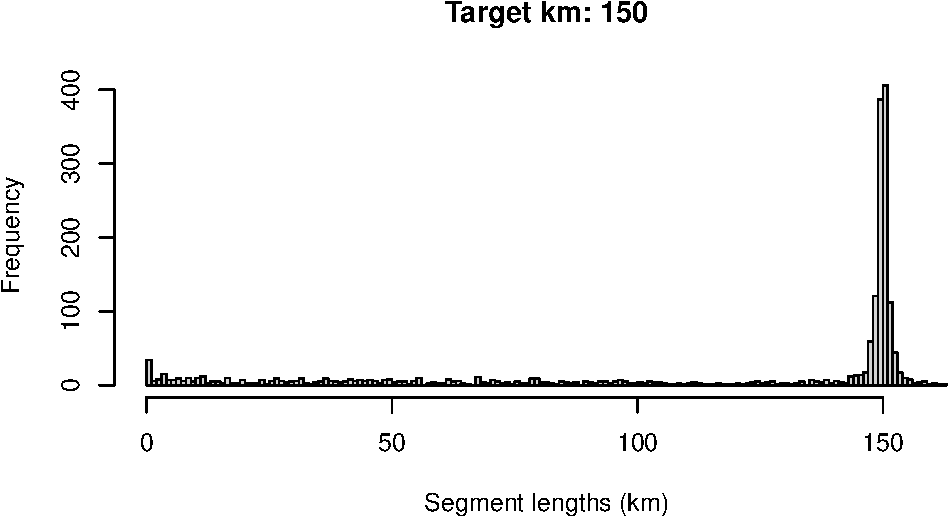
\includegraphics{figures/unnamed-chunk-43-1.pdf}

And the \texttt{das} slot holds the original \texttt{data.frame} of \texttt{DAS} data, modified slightly: the column \texttt{OnEffort} has been modified according to Beaufort range conditions, and the column \texttt{seg\_id} indicates which segment the event occurs within

\begin{Shaded}
\begin{Highlighting}[]
\NormalTok{cruz}\OperatorTok{$}\NormalTok{cohorts}\OperatorTok{$}\NormalTok{all}\OperatorTok{$}\NormalTok{das }\OperatorTok\StringTok{ }\NormalTok{names}
\NormalTok{ [}\DecValTok{1}\NormalTok{] }\StringTok{"Event"}            \StringTok{"DateTime"}         \StringTok{"Lat"}              \StringTok{"Lon"}             
\NormalTok{ [}\DecValTok{5}\NormalTok{] }\StringTok{"OnEffort"}         \StringTok{"Cruise"}           \StringTok{"Mode"}             \StringTok{"OffsetGMT"}       
\NormalTok{ [}\DecValTok{9}\NormalTok{] }\StringTok{"EffType"}          \StringTok{"ESWsides"}         \StringTok{"Course"}           \StringTok{"SpdKt"}           
\NormalTok{[}\DecValTok{13}\NormalTok{] }\StringTok{"Bft"}              \StringTok{"SwellHght"}        \StringTok{"WindSpdKt"}        \StringTok{"RainFog"}         
\NormalTok{[}\DecValTok{17}\NormalTok{] }\StringTok{"HorizSun"}         \StringTok{"VertSun"}          \StringTok{"Glare"}            \StringTok{"Vis"}             
\NormalTok{[}\DecValTok{21}\NormalTok{] }\StringTok{"ObsL"}             \StringTok{"Rec"}              \StringTok{"ObsR"}             \StringTok{"ObsInd"}          
\NormalTok{[}\DecValTok{25}\NormalTok{] }\StringTok{"Data1"}            \StringTok{"Data2"}            \StringTok{"Data3"}            \StringTok{"Data4"}           
\NormalTok{[}\DecValTok{29}\NormalTok{] }\StringTok{"Data5"}            \StringTok{"Data6"}            \StringTok{"Data7"}            \StringTok{"Data8"}           
\NormalTok{[}\DecValTok{33}\NormalTok{] }\StringTok{"Data9"}            \StringTok{"Data10"}           \StringTok{"Data11"}           \StringTok{"Data12"}          
\NormalTok{[}\DecValTok{37}\NormalTok{] }\StringTok{"EffortDot"}        \StringTok{"EventNum"}         \StringTok{"file_das"}         \StringTok{"line_num"}        
\NormalTok{[}\DecValTok{41}\NormalTok{] }\StringTok{"stratum_HI_EEZ"}   \StringTok{"stratum_OtherCNP"} \StringTok{"stratum_WHICEAS"}  \StringTok{"year"}            
\NormalTok{[}\DecValTok{45}\NormalTok{] }\StringTok{"month"}            \StringTok{"day"}              \StringTok{"yday"}             \StringTok{"km_int"}          
\NormalTok{[}\DecValTok{49}\NormalTok{] }\StringTok{"km_cum"}           \StringTok{"ship"}             \StringTok{"stratum"}          \StringTok{"seg_id"}          
\NormalTok{[}\DecValTok{53}\NormalTok{] }\StringTok{"use"}             
\end{Highlighting}
\end{Shaded}

The \texttt{segmentize()} function and its associated settings were designed to give researchers full control over how data are segmented, be it for design-based density analysis (which tend to use long segments of 100 km or more and allow for non-contiguous effort to be included in the same segment) or for habitat modeling (which tend to use short segments of 5 - 10 km and disallow non-contiguous effort to be pooled into the same segment). To demonstrate that versatility, checkout the \protect\hyperlink{segmentizing}{appendix on segmentizing}.

\hypertarget{process-sightings}{%
\subsection*{Process sightings}\label{process-sightings}}
\addcontentsline{toc}{subsection}{Process sightings}

To process sightings for each cohort of species, use the function \texttt{process\_sightings()}. This function has three basic steps: for each cohort, the function (1) prepares a sightings table using the function \texttt{das\_sight()} from \texttt{swfscDAS}; (2) filters those sightings to species codes specified for the cohort in your \texttt{settings} input; and (3) evaluates each of those sightings, asking if each should be included in the analysis according to your \texttt{settings}.

\begin{Shaded}
\begin{Highlighting}[]
\NormalTok{cruz <-}\StringTok{ }\KeywordTok{process_sightings}\NormalTok{(cruz)}
\end{Highlighting}
\end{Shaded}

The function produces a formatted dataset and adds it to a new \texttt{sightings} slot.

\begin{Shaded}
\begin{Highlighting}[]
\NormalTok{cruz}\OperatorTok{$}\NormalTok{cohorts}\OperatorTok{$}\NormalTok{all }\OperatorTok\StringTok{ }\NormalTok{names}
\NormalTok{[}\DecValTok{1}\NormalTok{] }\StringTok{"segments"}  \StringTok{"das"}       \StringTok{"sightings"}

\NormalTok{cruz}\OperatorTok{$}\NormalTok{cohorts}\OperatorTok{$}\NormalTok{bottlenose }\OperatorTok\StringTok{ }\NormalTok{names}
\NormalTok{[}\DecValTok{1}\NormalTok{] }\StringTok{"segments"}  \StringTok{"das"}       \StringTok{"sightings"}

\NormalTok{cruz}\OperatorTok{$}\NormalTok{cohorts}\OperatorTok{$}\NormalTok{spotted }\OperatorTok\StringTok{ }\NormalTok{names}
\NormalTok{[}\DecValTok{1}\NormalTok{] }\StringTok{"segments"}  \StringTok{"das"}       \StringTok{"sightings"}
\end{Highlighting}
\end{Shaded}

Note that the \texttt{sightings} table has a column named \texttt{included} (\texttt{TRUE} = yes, use it in the analysis). Any sightings that do not meet the inclusion criteria as specified in your settings will be \texttt{included\ =\ FALSE}, but they won't be removed from the data.

Since the sightings in each cohort are processed slightly differently according to the cohort's specific settings -- most importantly the species that will be included -- you should expect different numbers of included/excluded sightings in each cohort dataset:

\begin{Shaded}
\begin{Highlighting}[]
\NormalTok{cruz}\OperatorTok{$}\NormalTok{cohorts}\OperatorTok{$}\NormalTok{all}\OperatorTok{$}\NormalTok{sightings}\OperatorTok{$}\NormalTok{included }\OperatorTok\StringTok{ }\NormalTok{table}
\NormalTok{.}
\OtherTok{FALSE}  \OtherTok{TRUE} 
  \DecValTok{810}  \DecValTok{3122} 

\NormalTok{cruz}\OperatorTok{$}\NormalTok{cohorts}\OperatorTok{$}\NormalTok{bottlenose}\OperatorTok{$}\NormalTok{sightings}\OperatorTok{$}\NormalTok{included }\OperatorTok\StringTok{ }\NormalTok{table}
\NormalTok{.}
\OtherTok{FALSE}  \OtherTok{TRUE} 
  \DecValTok{114}   \DecValTok{408} 
\end{Highlighting}
\end{Shaded}

When this function's \texttt{verbose} argument is \texttt{TRUE} (the default), a message is printed each time a sighting does not meet the inclusion criteria.

\hypertarget{sightings-data-structure}{%
\subsubsection*{Sightings data structure}\label{sightings-data-structure}}
\addcontentsline{toc}{subsubsection}{Sightings data structure}

The \texttt{sightings} table has many other variables:

\begin{Shaded}
\begin{Highlighting}[]
\NormalTok{cruz}\OperatorTok{$}\NormalTok{cohorts}\OperatorTok{$}\NormalTok{all}\OperatorTok{$}\NormalTok{sightings }\OperatorTok\StringTok{ }\NormalTok{names}
\NormalTok{ [}\DecValTok{1}\NormalTok{] }\StringTok{"Event"}            \StringTok{"DateTime"}         \StringTok{"Lat"}              \StringTok{"Lon"}             
\NormalTok{ [}\DecValTok{5}\NormalTok{] }\StringTok{"OnEffort"}         \StringTok{"Cruise"}           \StringTok{"Mode"}             \StringTok{"OffsetGMT"}       
\NormalTok{ [}\DecValTok{9}\NormalTok{] }\StringTok{"EffType"}          \StringTok{"ESWsides"}         \StringTok{"Course"}           \StringTok{"SpdKt"}           
\NormalTok{[}\DecValTok{13}\NormalTok{] }\StringTok{"Bft"}              \StringTok{"SwellHght"}        \StringTok{"WindSpdKt"}        \StringTok{"RainFog"}         
\NormalTok{[}\DecValTok{17}\NormalTok{] }\StringTok{"HorizSun"}         \StringTok{"VertSun"}          \StringTok{"Glare"}            \StringTok{"Vis"}             
\NormalTok{[}\DecValTok{21}\NormalTok{] }\StringTok{"ObsL"}             \StringTok{"Rec"}              \StringTok{"ObsR"}             \StringTok{"ObsInd"}          
\NormalTok{[}\DecValTok{25}\NormalTok{] }\StringTok{"EffortDot"}        \StringTok{"EventNum"}         \StringTok{"file_das"}         \StringTok{"line_num"}        
\NormalTok{[}\DecValTok{29}\NormalTok{] }\StringTok{"stratum_HI_EEZ"}   \StringTok{"stratum_OtherCNP"} \StringTok{"stratum_WHICEAS"}  \StringTok{"year"}            
\NormalTok{[}\DecValTok{33}\NormalTok{] }\StringTok{"month"}            \StringTok{"day"}              \StringTok{"yday"}             \StringTok{"km_int"}          
\NormalTok{[}\DecValTok{37}\NormalTok{] }\StringTok{"km_cum"}           \StringTok{"ship"}             \StringTok{"stratum"}          \StringTok{"seg_id"}          
\NormalTok{[}\DecValTok{41}\NormalTok{] }\StringTok{"use"}              \StringTok{"SightNo"}          \StringTok{"Subgroup"}         \StringTok{"SightNoDaily"}    
\NormalTok{[}\DecValTok{45}\NormalTok{] }\StringTok{"Obs"}              \StringTok{"ObsStd"}           \StringTok{"Bearing"}          \StringTok{"Reticle"}         
\NormalTok{[}\DecValTok{49}\NormalTok{] }\StringTok{"DistNm"}           \StringTok{"Cue"}              \StringTok{"Method"}           \StringTok{"Photos"}          
\NormalTok{[}\DecValTok{53}\NormalTok{] }\StringTok{"Birds"}            \StringTok{"CalibSchool"}      \StringTok{"PhotosAerial"}     \StringTok{"Biopsy"}          
\NormalTok{[}\DecValTok{57}\NormalTok{] }\StringTok{"CourseSchool"}     \StringTok{"TurtleSp"}         \StringTok{"TurtleGs"}         \StringTok{"TurtleJFR"}       
\NormalTok{[}\DecValTok{61}\NormalTok{] }\StringTok{"TurtleAge"}        \StringTok{"TurtleCapt"}       \StringTok{"PinnipedSp"}       \StringTok{"PinnipedGs"}      
\NormalTok{[}\DecValTok{65}\NormalTok{] }\StringTok{"BoatType"}         \StringTok{"BoatGs"}           \StringTok{"PerpDistKm"}       \StringTok{"species"}         
\NormalTok{[}\DecValTok{69}\NormalTok{] }\StringTok{"best"}             \StringTok{"low"}              \StringTok{"high"}             \StringTok{"prob"}            
\NormalTok{[}\DecValTok{73}\NormalTok{] }\StringTok{"mixed"}            \StringTok{"ss_tot"}           \StringTok{"lnsstot"}          \StringTok{"ss_percent"}      
\NormalTok{[}\DecValTok{77}\NormalTok{] }\StringTok{"n_sp"}             \StringTok{"n_obs"}            \StringTok{"n_best"}           \StringTok{"n_low"}           
\NormalTok{[}\DecValTok{81}\NormalTok{] }\StringTok{"n_high"}           \StringTok{"calibr"}           \StringTok{"mixed_max"}        \StringTok{"spp_max"}         
\NormalTok{[}\DecValTok{85}\NormalTok{] }\StringTok{"included"}        
\end{Highlighting}
\end{Shaded}

Columns 42 onwards correspond to sightings information. Columns of note:

\begin{itemize}
\item
  \texttt{species} contains the species code. There is only one species-code per row (i.e, multi-species sightings have been expanded to multiple rows).
\item
  \texttt{best}, \texttt{low}, and \texttt{high} contain the refined group size estimates, averaged across observers and calibrated according to the cohort's settings specifications. For multi-species sightings, these numbers represent the number of individuals for the single species represented in the row (i.e., the original group size estimate has been scaled by the percentage attritbuted to this species).
\item
  The columns following those group size estimates (\texttt{prob} through \texttt{spp\_max}) detail how group sizes were estimated: \texttt{prob} indicates whether probable species codes were accepted; \texttt{mixed} indicates whether this species' sighting is part of a mixed-species sighting; \texttt{n\_sp} provides the number of species occurring in this sighitng; \texttt{n\_obs} gives the number of observers who contributed group size estimates; \texttt{n\_best} through \texttt{n\_high} gives the number of valid group size estimates given; and \texttt{calibr} indicates whether or not calibration was attempted for this sighting based on the settings (see next section); \texttt{mixed\_max} indicates whether this species was the most abundant in the sighting (if multi-species); \texttt{spp\_max} indicates the species code for the most abundant species in the sighting (if multi-species).
\item
  As explained above, the final column, \texttt{included}, indicates whether this species should be included in the analysis.
\end{itemize}

Here is a glimpse of the data:

\begin{Shaded}
\begin{Highlighting}[]
\NormalTok{cruz}\OperatorTok{$}\NormalTok{cohorts}\OperatorTok{$}\NormalTok{all}\OperatorTok{$}\NormalTok{sightings }\OperatorTok\StringTok{ }\NormalTok{glimpse}
\NormalTok{Rows}\OperatorTok{:}\StringTok{ }\DecValTok{3}\NormalTok{,}\DecValTok{932}
\NormalTok{Columns}\OperatorTok{:}\StringTok{ }\DecValTok{85}
\OperatorTok{$}\StringTok{ }\NormalTok{Event            }\OperatorTok{<}\NormalTok{chr}\OperatorTok{>}\StringTok{ "S"}\NormalTok{, }\StringTok{"S"}\NormalTok{, }\StringTok{"S"}\NormalTok{, }\StringTok{"S"}\NormalTok{, }\StringTok{"S"}\NormalTok{, }\StringTok{"S"}\NormalTok{, }\StringTok{"S"}\NormalTok{, }\StringTok{"S"}\NormalTok{, }\StringTok{"S"}\NormalTok{, }\StringTok{"S"}\NormalTok{, }\StringTok{"S"}\OperatorTok{~}
\ErrorTok{$}\StringTok{ }\NormalTok{DateTime         }\OperatorTok{<}\NormalTok{dttm}\OperatorTok{>}\StringTok{ }\DecValTok{1986-11-26} \DecValTok{09}\OperatorTok{:}\DecValTok{00}\OperatorTok{:}\DecValTok{00}\NormalTok{, }\DecValTok{1986-11-26} \DecValTok{14}\OperatorTok{:}\DecValTok{40}\OperatorTok{:}\DecValTok{00}\NormalTok{, }\DecValTok{1986-11-26}\OperatorTok{~}
\ErrorTok{$}\StringTok{ }\NormalTok{Lat              }\OperatorTok{<}\NormalTok{dbl}\OperatorTok{>}\StringTok{ }\FloatTok{4.983333}\NormalTok{, }\FloatTok{5.616667}\NormalTok{, }\FloatTok{5.866667}\NormalTok{, }\FloatTok{7.050000}\NormalTok{, }\FloatTok{7.466667}\NormalTok{, }\FloatTok{9.4}\OperatorTok{~}
\ErrorTok{$}\StringTok{ }\NormalTok{Lon              }\OperatorTok{<}\NormalTok{dbl}\OperatorTok{>}\StringTok{ }\FloatTok{-120.9500}\NormalTok{, }\FloatTok{-121.6667}\NormalTok{, }\FloatTok{-121.9833}\NormalTok{, }\FloatTok{-123.5000}\NormalTok{, }\FloatTok{-123.9167}\OperatorTok{~}
\ErrorTok{$}\StringTok{ }\NormalTok{OnEffort         }\OperatorTok{<}\NormalTok{lgl}\OperatorTok{>}\StringTok{ }\OtherTok{TRUE}\NormalTok{, }\OtherTok{TRUE}\NormalTok{, }\OtherTok{TRUE}\NormalTok{, }\OtherTok{TRUE}\NormalTok{, }\OtherTok{TRUE}\NormalTok{, }\OtherTok{TRUE}\NormalTok{, }\OtherTok{TRUE}\NormalTok{, }\OtherTok{TRUE}\NormalTok{, }\OtherTok{TRUE}\NormalTok{,}\OperatorTok{~}
\ErrorTok{$}\StringTok{ }\NormalTok{Cruise           }\OperatorTok{<}\NormalTok{dbl}\OperatorTok{>}\StringTok{ }\DecValTok{989}\NormalTok{, }\DecValTok{989}\NormalTok{, }\DecValTok{989}\NormalTok{, }\DecValTok{989}\NormalTok{, }\DecValTok{989}\NormalTok{, }\DecValTok{989}\NormalTok{, }\DecValTok{989}\NormalTok{, }\DecValTok{989}\NormalTok{, }\DecValTok{989}\NormalTok{, }\DecValTok{989}\NormalTok{, }\DecValTok{989}\OperatorTok{~}
\ErrorTok{$}\StringTok{ }\NormalTok{Mode             }\OperatorTok{<}\NormalTok{chr}\OperatorTok{>}\StringTok{ "C"}\NormalTok{, }\StringTok{"C"}\NormalTok{, }\StringTok{"C"}\NormalTok{, }\StringTok{"C"}\NormalTok{, }\StringTok{"C"}\NormalTok{, }\StringTok{"C"}\NormalTok{, }\StringTok{"C"}\NormalTok{, }\StringTok{"C"}\NormalTok{, }\StringTok{"C"}\NormalTok{, }\StringTok{"C"}\NormalTok{, }\StringTok{"C"}\OperatorTok{~}
\ErrorTok{$}\StringTok{ }\NormalTok{OffsetGMT        }\OperatorTok{<}\NormalTok{int}\OperatorTok{>}\StringTok{ }\OtherTok{NA}\NormalTok{, }\OtherTok{NA}\NormalTok{, }\OtherTok{NA}\NormalTok{, }\OtherTok{NA}\NormalTok{, }\OtherTok{NA}\NormalTok{, }\OtherTok{NA}\NormalTok{, }\OtherTok{NA}\NormalTok{, }\OtherTok{NA}\NormalTok{, }\OtherTok{NA}\NormalTok{, }\OtherTok{NA}\NormalTok{, }\OtherTok{NA}\NormalTok{, }\OtherTok{NA}\NormalTok{, }\OtherTok{NA}\NormalTok{, N}\OperatorTok{~}
\ErrorTok{$}\StringTok{ }\NormalTok{EffType          }\OperatorTok{<}\NormalTok{chr}\OperatorTok{>}\StringTok{ "S"}\NormalTok{, }\StringTok{"S"}\NormalTok{, }\StringTok{"S"}\NormalTok{, }\StringTok{"S"}\NormalTok{, }\StringTok{"S"}\NormalTok{, }\StringTok{"S"}\NormalTok{, }\StringTok{"S"}\NormalTok{, }\StringTok{"S"}\NormalTok{, }\StringTok{"S"}\NormalTok{, }\StringTok{"S"}\NormalTok{, }\StringTok{"S"}\OperatorTok{~}
\ErrorTok{$}\StringTok{ }\NormalTok{ESWsides         }\OperatorTok{<}\NormalTok{dbl}\OperatorTok{>}\StringTok{ }\DecValTok{2}\NormalTok{, }\DecValTok{2}\NormalTok{, }\DecValTok{2}\NormalTok{, }\DecValTok{2}\NormalTok{, }\DecValTok{2}\NormalTok{, }\DecValTok{2}\NormalTok{, }\DecValTok{2}\NormalTok{, }\DecValTok{2}\NormalTok{, }\DecValTok{2}\NormalTok{, }\DecValTok{2}\NormalTok{, }\DecValTok{2}\NormalTok{, }\DecValTok{2}\NormalTok{, }\DecValTok{2}\NormalTok{, }\DecValTok{2}\NormalTok{, }\DecValTok{2}\NormalTok{, }\DecValTok{2}\NormalTok{, }\DecValTok{2}\NormalTok{, }\DecValTok{2}\NormalTok{,}\OperatorTok{~}
\ErrorTok{$}\StringTok{ }\NormalTok{Course           }\OperatorTok{<}\NormalTok{dbl}\OperatorTok{>}\StringTok{ }\DecValTok{310}\NormalTok{, }\DecValTok{316}\NormalTok{, }\DecValTok{313}\NormalTok{, }\DecValTok{310}\NormalTok{, }\DecValTok{310}\NormalTok{, }\DecValTok{305}\NormalTok{, }\DecValTok{305}\NormalTok{, }\DecValTok{305}\NormalTok{, }\DecValTok{305}\NormalTok{, }\DecValTok{305}\NormalTok{, }\DecValTok{305}\OperatorTok{~}
\ErrorTok{$}\StringTok{ }\NormalTok{SpdKt            }\OperatorTok{<}\NormalTok{dbl}\OperatorTok{>}\StringTok{ }\FloatTok{10.2}\NormalTok{, }\FloatTok{9.9}\NormalTok{, }\FloatTok{9.6}\NormalTok{, }\FloatTok{10.2}\NormalTok{, }\FloatTok{10.3}\NormalTok{, }\FloatTok{9.8}\NormalTok{, }\FloatTok{9.8}\NormalTok{, }\FloatTok{9.6}\NormalTok{, }\FloatTok{10.1}\NormalTok{, }\FloatTok{10.1}\OperatorTok{~}
\ErrorTok{$}\StringTok{ }\NormalTok{Bft              }\OperatorTok{<}\NormalTok{dbl}\OperatorTok{>}\StringTok{ }\DecValTok{4}\NormalTok{, }\DecValTok{4}\NormalTok{, }\DecValTok{4}\NormalTok{, }\DecValTok{3}\NormalTok{, }\DecValTok{3}\NormalTok{, }\DecValTok{2}\NormalTok{, }\DecValTok{2}\NormalTok{, }\DecValTok{2}\NormalTok{, }\DecValTok{1}\NormalTok{, }\DecValTok{1}\NormalTok{, }\DecValTok{1}\NormalTok{, }\DecValTok{4}\NormalTok{, }\DecValTok{5}\NormalTok{, }\DecValTok{4}\NormalTok{, }\DecValTok{4}\NormalTok{, }\DecValTok{3}\NormalTok{, }\DecValTok{1}\NormalTok{, }\DecValTok{2}\NormalTok{,}\OperatorTok{~}
\ErrorTok{$}\StringTok{ }\NormalTok{SwellHght        }\OperatorTok{<}\NormalTok{dbl}\OperatorTok{>}\StringTok{ }\OtherTok{NA}\NormalTok{, }\OtherTok{NA}\NormalTok{, }\OtherTok{NA}\NormalTok{, }\OtherTok{NA}\NormalTok{, }\OtherTok{NA}\NormalTok{, }\OtherTok{NA}\NormalTok{, }\OtherTok{NA}\NormalTok{, }\OtherTok{NA}\NormalTok{, }\OtherTok{NA}\NormalTok{, }\OtherTok{NA}\NormalTok{, }\OtherTok{NA}\NormalTok{, }\OtherTok{NA}\NormalTok{, }\OtherTok{NA}\NormalTok{, N}\OperatorTok{~}
\ErrorTok{$}\StringTok{ }\NormalTok{WindSpdKt        }\OperatorTok{<}\NormalTok{dbl}\OperatorTok{>}\StringTok{ }\OtherTok{NA}\NormalTok{, }\OtherTok{NA}\NormalTok{, }\OtherTok{NA}\NormalTok{, }\OtherTok{NA}\NormalTok{, }\OtherTok{NA}\NormalTok{, }\OtherTok{NA}\NormalTok{, }\OtherTok{NA}\NormalTok{, }\OtherTok{NA}\NormalTok{, }\OtherTok{NA}\NormalTok{, }\OtherTok{NA}\NormalTok{, }\OtherTok{NA}\NormalTok{, }\OtherTok{NA}\NormalTok{, }\OtherTok{NA}\NormalTok{, N}\OperatorTok{~}
\ErrorTok{$}\StringTok{ }\NormalTok{RainFog          }\OperatorTok{<}\NormalTok{dbl}\OperatorTok{>}\StringTok{ }\DecValTok{1}\NormalTok{, }\DecValTok{1}\NormalTok{, }\DecValTok{1}\NormalTok{, }\DecValTok{1}\NormalTok{, }\DecValTok{1}\NormalTok{, }\DecValTok{1}\NormalTok{, }\DecValTok{1}\NormalTok{, }\DecValTok{1}\NormalTok{, }\DecValTok{1}\NormalTok{, }\DecValTok{1}\NormalTok{, }\DecValTok{1}\NormalTok{, }\DecValTok{1}\NormalTok{, }\DecValTok{1}\NormalTok{, }\DecValTok{1}\NormalTok{, }\DecValTok{1}\NormalTok{, }\DecValTok{1}\NormalTok{, }\DecValTok{1}\NormalTok{, }\DecValTok{1}\NormalTok{,}\OperatorTok{~}
\ErrorTok{$}\StringTok{ }\NormalTok{HorizSun         }\OperatorTok{<}\NormalTok{dbl}\OperatorTok{>}\StringTok{ }\DecValTok{6}\NormalTok{, }\DecValTok{9}\NormalTok{, }\DecValTok{10}\NormalTok{, }\OtherTok{NA}\NormalTok{, }\DecValTok{7}\NormalTok{, }\DecValTok{5}\NormalTok{, }\DecValTok{5}\NormalTok{, }\DecValTok{7}\NormalTok{, }\DecValTok{8}\NormalTok{, }\DecValTok{8}\NormalTok{, }\DecValTok{8}\NormalTok{, }\DecValTok{3}\NormalTok{, }\DecValTok{5}\NormalTok{, }\OtherTok{NA}\NormalTok{, }\DecValTok{4}\NormalTok{, }\OtherTok{NA}\NormalTok{, N}\OperatorTok{~}
\ErrorTok{$}\StringTok{ }\NormalTok{VertSun          }\OperatorTok{<}\NormalTok{dbl}\OperatorTok{>}\StringTok{ }\DecValTok{2}\NormalTok{, }\DecValTok{1}\NormalTok{, }\DecValTok{3}\NormalTok{, }\OtherTok{NA}\NormalTok{, }\DecValTok{1}\NormalTok{, }\DecValTok{3}\NormalTok{, }\DecValTok{3}\NormalTok{, }\DecValTok{1}\NormalTok{, }\DecValTok{1}\NormalTok{, }\DecValTok{1}\NormalTok{, }\DecValTok{1}\NormalTok{, }\DecValTok{2}\NormalTok{, }\DecValTok{1}\NormalTok{, }\OtherTok{NA}\NormalTok{, }\DecValTok{1}\NormalTok{, }\OtherTok{NA}\NormalTok{, }\OtherTok{NA}\OperatorTok{~}
\ErrorTok{$}\StringTok{ }\NormalTok{Glare            }\OperatorTok{<}\NormalTok{lgl}\OperatorTok{>}\StringTok{ }\OtherTok{FALSE}\NormalTok{, }\OtherTok{FALSE}\NormalTok{, }\OtherTok{FALSE}\NormalTok{, }\OtherTok{NA}\NormalTok{, }\OtherTok{FALSE}\NormalTok{, }\OtherTok{FALSE}\NormalTok{, }\OtherTok{FALSE}\NormalTok{, }\OtherTok{FALSE}\NormalTok{, }\OperatorTok{~}
\ErrorTok{$}\StringTok{ }\NormalTok{Vis              }\OperatorTok{<}\NormalTok{dbl}\OperatorTok{>}\StringTok{ }\OtherTok{NA}\NormalTok{, }\OtherTok{NA}\NormalTok{, }\OtherTok{NA}\NormalTok{, }\OtherTok{NA}\NormalTok{, }\OtherTok{NA}\NormalTok{, }\OtherTok{NA}\NormalTok{, }\OtherTok{NA}\NormalTok{, }\OtherTok{NA}\NormalTok{, }\OtherTok{NA}\NormalTok{, }\OtherTok{NA}\NormalTok{, }\OtherTok{NA}\NormalTok{, }\OtherTok{NA}\NormalTok{, }\OtherTok{NA}\NormalTok{, N}\OperatorTok{~}
\ErrorTok{$}\StringTok{ }\NormalTok{ObsL             }\OperatorTok{<}\NormalTok{chr}\OperatorTok{>}\StringTok{ "004"}\NormalTok{, }\StringTok{"022"}\NormalTok{, }\StringTok{"056"}\NormalTok{, }\StringTok{"056"}\NormalTok{, }\StringTok{"004"}\NormalTok{, }\StringTok{"031"}\NormalTok{, }\StringTok{"031"}\NormalTok{, }\StringTok{"004~}
\StringTok{$ Rec              <chr> "}\DecValTok{056}\StringTok{", "}\DecValTok{031}\StringTok{", "}\DecValTok{062}\StringTok{", "}\DecValTok{062}\StringTok{", "}\DecValTok{056}\StringTok{", "}\DecValTok{022}\StringTok{", "}\DecValTok{022}\StringTok{", "}\DecValTok{056}\OperatorTok{~}
\ErrorTok{$}\StringTok{ }\NormalTok{ObsR             }\OperatorTok{<}\NormalTok{chr}\OperatorTok{>}\StringTok{ "062"}\NormalTok{, }\StringTok{"057"}\NormalTok{, }\StringTok{"004"}\NormalTok{, }\StringTok{"004"}\NormalTok{, }\StringTok{"062"}\NormalTok{, }\StringTok{"057"}\NormalTok{, }\StringTok{"057"}\NormalTok{, }\StringTok{"062~}
\StringTok{$ ObsInd           <chr> NA, NA, NA, NA, NA, NA, NA, NA, NA, NA, NA, NA, NA, N~}
\StringTok{$ EffortDot        <lgl> TRUE, TRUE, TRUE, TRUE, TRUE, TRUE, TRUE, TRUE, TRUE,~}
\StringTok{$ EventNum         <chr> "}\DecValTok{18}\StringTok{", "}\DecValTok{43}\StringTok{", "}\DecValTok{59}\StringTok{", "}\DecValTok{9}\StringTok{", "}\DecValTok{32}\StringTok{", "}\DecValTok{10}\StringTok{", "}\DecValTok{10}\StringTok{", "}\DecValTok{22}\StringTok{", "}\DecValTok{34}\StringTok{", ~}
\StringTok{$ file_das         <chr> "}\NormalTok{CenPac1986}\DecValTok{-2020}\NormalTok{_Final_alb.das}\StringTok{", "}\NormalTok{CenPac1986}\DecValTok{-2020}\NormalTok{_Fin}\OperatorTok{~}
\ErrorTok{$}\StringTok{ }\NormalTok{line_num         }\OperatorTok{<}\NormalTok{int}\OperatorTok{>}\StringTok{ }\DecValTok{10295}\NormalTok{, }\DecValTok{10321}\NormalTok{, }\DecValTok{10340}\NormalTok{, }\DecValTok{10358}\NormalTok{, }\DecValTok{10384}\NormalTok{, }\DecValTok{10451}\NormalTok{, }\DecValTok{10451}\NormalTok{, }\DecValTok{1046}\OperatorTok{~}
\ErrorTok{$}\StringTok{ }\NormalTok{stratum_HI_EEZ   }\OperatorTok{<}\NormalTok{lgl}\OperatorTok{>}\StringTok{ }\OtherTok{FALSE}\NormalTok{, }\OtherTok{FALSE}\NormalTok{, }\OtherTok{FALSE}\NormalTok{, }\OtherTok{FALSE}\NormalTok{, }\OtherTok{FALSE}\NormalTok{, }\OtherTok{FALSE}\NormalTok{, }\OtherTok{FALSE}\NormalTok{, FALS}\OperatorTok{~}
\ErrorTok{$}\StringTok{ }\NormalTok{stratum_OtherCNP }\OperatorTok{<}\NormalTok{lgl}\OperatorTok{>}\StringTok{ }\OtherTok{TRUE}\NormalTok{, }\OtherTok{TRUE}\NormalTok{, }\OtherTok{TRUE}\NormalTok{, }\OtherTok{TRUE}\NormalTok{, }\OtherTok{TRUE}\NormalTok{, }\OtherTok{TRUE}\NormalTok{, }\OtherTok{TRUE}\NormalTok{, }\OtherTok{TRUE}\NormalTok{, }\OtherTok{TRUE}\NormalTok{,}\OperatorTok{~}
\ErrorTok{$}\StringTok{ }\NormalTok{stratum_WHICEAS  }\OperatorTok{<}\NormalTok{lgl}\OperatorTok{>}\StringTok{ }\OtherTok{FALSE}\NormalTok{, }\OtherTok{FALSE}\NormalTok{, }\OtherTok{FALSE}\NormalTok{, }\OtherTok{FALSE}\NormalTok{, }\OtherTok{FALSE}\NormalTok{, }\OtherTok{FALSE}\NormalTok{, }\OtherTok{FALSE}\NormalTok{, FALS}\OperatorTok{~}
\ErrorTok{$}\StringTok{ }\NormalTok{year             }\OperatorTok{<}\NormalTok{dbl}\OperatorTok{>}\StringTok{ }\DecValTok{1986}\NormalTok{, }\DecValTok{1986}\NormalTok{, }\DecValTok{1986}\NormalTok{, }\DecValTok{1986}\NormalTok{, }\DecValTok{1986}\NormalTok{, }\DecValTok{1986}\NormalTok{, }\DecValTok{1986}\NormalTok{, }\DecValTok{1986}\NormalTok{, }\DecValTok{1986}\NormalTok{,}\OperatorTok{~}
\ErrorTok{$}\StringTok{ }\NormalTok{month            }\OperatorTok{<}\NormalTok{dbl}\OperatorTok{>}\StringTok{ }\DecValTok{11}\NormalTok{, }\DecValTok{11}\NormalTok{, }\DecValTok{11}\NormalTok{, }\DecValTok{11}\NormalTok{, }\DecValTok{11}\NormalTok{, }\DecValTok{11}\NormalTok{, }\DecValTok{11}\NormalTok{, }\DecValTok{11}\NormalTok{, }\DecValTok{11}\NormalTok{, }\DecValTok{11}\NormalTok{, }\DecValTok{11}\NormalTok{, }\DecValTok{11}\NormalTok{, }\DecValTok{11}\NormalTok{, }\DecValTok{1}\OperatorTok{~}
\ErrorTok{$}\StringTok{ }\NormalTok{day              }\OperatorTok{<}\NormalTok{int}\OperatorTok{>}\StringTok{ }\DecValTok{26}\NormalTok{, }\DecValTok{26}\NormalTok{, }\DecValTok{26}\NormalTok{, }\DecValTok{27}\NormalTok{, }\DecValTok{27}\NormalTok{, }\DecValTok{28}\NormalTok{, }\DecValTok{28}\NormalTok{, }\DecValTok{28}\NormalTok{, }\DecValTok{28}\NormalTok{, }\DecValTok{28}\NormalTok{, }\DecValTok{28}\NormalTok{, }\DecValTok{29}\NormalTok{, }\DecValTok{29}\NormalTok{, }\DecValTok{3}\OperatorTok{~}
\ErrorTok{$}\StringTok{ }\NormalTok{yday             }\OperatorTok{<}\NormalTok{dbl}\OperatorTok{>}\StringTok{ }\DecValTok{330}\NormalTok{, }\DecValTok{330}\NormalTok{, }\DecValTok{330}\NormalTok{, }\DecValTok{331}\NormalTok{, }\DecValTok{331}\NormalTok{, }\DecValTok{332}\NormalTok{, }\DecValTok{332}\NormalTok{, }\DecValTok{332}\NormalTok{, }\DecValTok{332}\NormalTok{, }\DecValTok{332}\NormalTok{, }\DecValTok{332}\OperatorTok{~}
\ErrorTok{$}\StringTok{ }\NormalTok{km_int           }\OperatorTok{<}\NormalTok{dbl}\OperatorTok{>}\StringTok{ }\DecValTok{0}\NormalTok{, }\DecValTok{0}\NormalTok{, }\DecValTok{0}\NormalTok{, }\DecValTok{0}\NormalTok{, }\DecValTok{0}\NormalTok{, }\DecValTok{0}\NormalTok{, }\DecValTok{0}\NormalTok{, }\DecValTok{0}\NormalTok{, }\DecValTok{0}\NormalTok{, }\DecValTok{0}\NormalTok{, }\DecValTok{0}\NormalTok{, }\DecValTok{0}\NormalTok{, }\DecValTok{0}\NormalTok{, }\DecValTok{0}\NormalTok{, }\DecValTok{0}\NormalTok{, }\DecValTok{0}\NormalTok{, }\DecValTok{0}\NormalTok{, }\DecValTok{0}\NormalTok{,}\OperatorTok{~}
\ErrorTok{$}\StringTok{ }\NormalTok{km_cum           }\OperatorTok{<}\NormalTok{dbl}\OperatorTok{>}\StringTok{ }\FloatTok{64.38787}\NormalTok{, }\FloatTok{172.92124}\NormalTok{, }\FloatTok{221.24918}\NormalTok{, }\FloatTok{248.23899}\NormalTok{, }\FloatTok{317.83407}\NormalTok{,}\OperatorTok{~}
\ErrorTok{$}\StringTok{ }\NormalTok{ship             }\OperatorTok{<}\NormalTok{chr}\OperatorTok{>}\StringTok{ "DSJ"}\NormalTok{, }\StringTok{"DSJ"}\NormalTok{, }\StringTok{"DSJ"}\NormalTok{, }\StringTok{"DSJ"}\NormalTok{, }\StringTok{"DSJ"}\NormalTok{, }\StringTok{"DSJ"}\NormalTok{, }\StringTok{"DSJ"}\NormalTok{, }\StringTok{"DSJ~}
\StringTok{$ stratum          <chr> "}\NormalTok{OtherCNP}\StringTok{", "}\NormalTok{OtherCNP}\StringTok{", "}\NormalTok{OtherCNP}\StringTok{", "}\NormalTok{OtherCNP}\StringTok{", "}\NormalTok{Othe}\OperatorTok{~}
\ErrorTok{$}\StringTok{ }\NormalTok{seg_id           }\OperatorTok{<}\NormalTok{int}\OperatorTok{>}\StringTok{ }\DecValTok{34}\NormalTok{, }\DecValTok{35}\NormalTok{, }\DecValTok{35}\NormalTok{, }\DecValTok{35}\NormalTok{, }\DecValTok{36}\NormalTok{, }\DecValTok{37}\NormalTok{, }\DecValTok{37}\NormalTok{, }\DecValTok{37}\NormalTok{, }\DecValTok{37}\NormalTok{, }\DecValTok{37}\NormalTok{, }\DecValTok{29}\NormalTok{, }\DecValTok{38}\NormalTok{, }\DecValTok{38}\NormalTok{, }\DecValTok{3}\OperatorTok{~}
\ErrorTok{$}\StringTok{ }\NormalTok{use              }\OperatorTok{<}\NormalTok{lgl}\OperatorTok{>}\StringTok{ }\OtherTok{TRUE}\NormalTok{, }\OtherTok{TRUE}\NormalTok{, }\OtherTok{TRUE}\NormalTok{, }\OtherTok{TRUE}\NormalTok{, }\OtherTok{TRUE}\NormalTok{, }\OtherTok{TRUE}\NormalTok{, }\OtherTok{TRUE}\NormalTok{, }\OtherTok{TRUE}\NormalTok{, }\OtherTok{TRUE}\NormalTok{,}\OperatorTok{~}
\ErrorTok{$}\StringTok{ }\NormalTok{SightNo          }\OperatorTok{<}\NormalTok{chr}\OperatorTok{>}\StringTok{ "01"}\NormalTok{, }\StringTok{"02"}\NormalTok{, }\StringTok{"03"}\NormalTok{, }\StringTok{"01"}\NormalTok{, }\StringTok{"02"}\NormalTok{, }\StringTok{"01"}\NormalTok{, }\StringTok{"01"}\NormalTok{, }\StringTok{"02"}\NormalTok{, }\StringTok{"03"}\NormalTok{,}\OperatorTok{~}
\ErrorTok{$}\StringTok{ }\NormalTok{Subgroup         }\OperatorTok{<}\NormalTok{chr}\OperatorTok{>}\StringTok{ }\OtherTok{NA}\NormalTok{, }\OtherTok{NA}\NormalTok{, }\OtherTok{NA}\NormalTok{, }\OtherTok{NA}\NormalTok{, }\OtherTok{NA}\NormalTok{, }\OtherTok{NA}\NormalTok{, }\OtherTok{NA}\NormalTok{, }\OtherTok{NA}\NormalTok{, }\OtherTok{NA}\NormalTok{, }\OtherTok{NA}\NormalTok{, }\OtherTok{NA}\NormalTok{, }\OtherTok{NA}\NormalTok{, }\OtherTok{NA}\NormalTok{, N}\OperatorTok{~}
\ErrorTok{$}\StringTok{ }\NormalTok{SightNoDaily     }\OperatorTok{<}\NormalTok{chr}\OperatorTok{>}\StringTok{ "19861126_1"}\NormalTok{, }\StringTok{"19861126_2"}\NormalTok{, }\StringTok{"19861126_3"}\NormalTok{, }\StringTok{"19861127_1~}
\StringTok{$ Obs              <chr> "}\DecValTok{004}\StringTok{", "}\DecValTok{057}\StringTok{", "}\DecValTok{004}\StringTok{", "}\DecValTok{056}\StringTok{", "}\DecValTok{004}\StringTok{", "}\DecValTok{031}\StringTok{", "}\DecValTok{031}\StringTok{", "}\DecValTok{004}\OperatorTok{~}
\ErrorTok{$}\StringTok{ }\NormalTok{ObsStd           }\OperatorTok{<}\NormalTok{lgl}\OperatorTok{>}\StringTok{ }\OtherTok{TRUE}\NormalTok{, }\OtherTok{TRUE}\NormalTok{, }\OtherTok{TRUE}\NormalTok{, }\OtherTok{TRUE}\NormalTok{, }\OtherTok{TRUE}\NormalTok{, }\OtherTok{TRUE}\NormalTok{, }\OtherTok{TRUE}\NormalTok{, }\OtherTok{TRUE}\NormalTok{, }\OtherTok{TRUE}\NormalTok{,}\OperatorTok{~}
\ErrorTok{$}\StringTok{ }\NormalTok{Bearing          }\OperatorTok{<}\NormalTok{dbl}\OperatorTok{>}\StringTok{ }\DecValTok{335}\NormalTok{, }\DecValTok{354}\NormalTok{, }\DecValTok{336}\NormalTok{, }\DecValTok{18}\NormalTok{, }\DecValTok{332}\NormalTok{, }\DecValTok{333}\NormalTok{, }\DecValTok{333}\NormalTok{, }\DecValTok{6}\NormalTok{, }\DecValTok{312}\NormalTok{, }\DecValTok{312}\NormalTok{, }\DecValTok{38}\NormalTok{, }\DecValTok{80}\OperatorTok{~}
\ErrorTok{$}\StringTok{ }\NormalTok{Reticle          }\OperatorTok{<}\NormalTok{dbl}\OperatorTok{>}\StringTok{ }\FloatTok{8.41}\NormalTok{, }\FloatTok{3.88}\NormalTok{, }\FloatTok{0.50}\NormalTok{, }\FloatTok{11.40}\NormalTok{, }\FloatTok{0.80}\NormalTok{, }\FloatTok{0.30}\NormalTok{, }\FloatTok{0.30}\NormalTok{, }\FloatTok{2.98}\NormalTok{, }\FloatTok{0.40}\OperatorTok{~}
\ErrorTok{$}\StringTok{ }\NormalTok{DistNm           }\OperatorTok{<}\NormalTok{dbl}\OperatorTok{>}\StringTok{ }\FloatTok{0.4}\NormalTok{, }\FloatTok{0.8}\NormalTok{, }\FloatTok{3.2}\NormalTok{, }\FloatTok{0.3}\NormalTok{, }\FloatTok{2.5}\NormalTok{, }\FloatTok{3.8}\NormalTok{, }\FloatTok{3.8}\NormalTok{, }\FloatTok{1.0}\NormalTok{, }\FloatTok{3.5}\NormalTok{, }\FloatTok{3.5}\NormalTok{, }\FloatTok{7.0}\OperatorTok{~}
\ErrorTok{$}\StringTok{ }\NormalTok{Cue              }\OperatorTok{<}\NormalTok{dbl}\OperatorTok{>}\StringTok{ }\DecValTok{3}\NormalTok{, }\DecValTok{3}\NormalTok{, }\DecValTok{2}\NormalTok{, }\DecValTok{2}\NormalTok{, }\DecValTok{3}\NormalTok{, }\DecValTok{3}\NormalTok{, }\DecValTok{3}\NormalTok{, }\DecValTok{3}\NormalTok{, }\DecValTok{2}\NormalTok{, }\DecValTok{2}\NormalTok{, }\DecValTok{3}\NormalTok{, }\DecValTok{3}\NormalTok{, }\DecValTok{6}\NormalTok{, }\DecValTok{6}\NormalTok{, }\DecValTok{3}\NormalTok{, }\DecValTok{2}\NormalTok{, }\DecValTok{3}\NormalTok{, }\DecValTok{2}\NormalTok{,}\OperatorTok{~}
\ErrorTok{$}\StringTok{ }\NormalTok{Method           }\OperatorTok{<}\NormalTok{dbl}\OperatorTok{>}\StringTok{ }\DecValTok{4}\NormalTok{, }\DecValTok{4}\NormalTok{, }\DecValTok{4}\NormalTok{, }\DecValTok{4}\NormalTok{, }\DecValTok{4}\NormalTok{, }\DecValTok{4}\NormalTok{, }\DecValTok{4}\NormalTok{, }\DecValTok{4}\NormalTok{, }\DecValTok{4}\NormalTok{, }\DecValTok{4}\NormalTok{, }\DecValTok{4}\NormalTok{, }\DecValTok{4}\NormalTok{, }\DecValTok{4}\NormalTok{, }\DecValTok{4}\NormalTok{, }\DecValTok{4}\NormalTok{, }\DecValTok{4}\NormalTok{, }\DecValTok{4}\NormalTok{, }\DecValTok{4}\NormalTok{,}\OperatorTok{~}
\ErrorTok{$}\StringTok{ }\NormalTok{Photos           }\OperatorTok{<}\NormalTok{chr}\OperatorTok{>}\StringTok{ }\OtherTok{NA}\NormalTok{, }\OtherTok{NA}\NormalTok{, }\OtherTok{NA}\NormalTok{, }\OtherTok{NA}\NormalTok{, }\OtherTok{NA}\NormalTok{, }\OtherTok{NA}\NormalTok{, }\OtherTok{NA}\NormalTok{, }\OtherTok{NA}\NormalTok{, }\OtherTok{NA}\NormalTok{, }\OtherTok{NA}\NormalTok{, }\OtherTok{NA}\NormalTok{, }\OtherTok{NA}\NormalTok{, }\OtherTok{NA}\NormalTok{, N}\OperatorTok{~}
\ErrorTok{$}\StringTok{ }\NormalTok{Birds            }\OperatorTok{<}\NormalTok{chr}\OperatorTok{>}\StringTok{ "N"}\NormalTok{, }\StringTok{"N"}\NormalTok{, }\StringTok{"N"}\NormalTok{, }\StringTok{"N"}\NormalTok{, }\StringTok{"N"}\NormalTok{, }\StringTok{"Y"}\NormalTok{, }\StringTok{"Y"}\NormalTok{, }\StringTok{"N"}\NormalTok{, }\StringTok{"Y"}\NormalTok{, }\StringTok{"Y"}\NormalTok{, }\StringTok{"N"}\OperatorTok{~}
\ErrorTok{$}\StringTok{ }\NormalTok{CalibSchool      }\OperatorTok{<}\NormalTok{chr}\OperatorTok{>}\StringTok{ }\OtherTok{NA}\NormalTok{, }\OtherTok{NA}\NormalTok{, }\OtherTok{NA}\NormalTok{, }\OtherTok{NA}\NormalTok{, }\OtherTok{NA}\NormalTok{, }\OtherTok{NA}\NormalTok{, }\OtherTok{NA}\NormalTok{, }\OtherTok{NA}\NormalTok{, }\OtherTok{NA}\NormalTok{, }\OtherTok{NA}\NormalTok{, }\OtherTok{NA}\NormalTok{, }\OtherTok{NA}\NormalTok{, }\OtherTok{NA}\NormalTok{, N}\OperatorTok{~}
\ErrorTok{$}\StringTok{ }\NormalTok{PhotosAerial     }\OperatorTok{<}\NormalTok{chr}\OperatorTok{>}\StringTok{ }\OtherTok{NA}\NormalTok{, }\OtherTok{NA}\NormalTok{, }\OtherTok{NA}\NormalTok{, }\OtherTok{NA}\NormalTok{, }\OtherTok{NA}\NormalTok{, }\OtherTok{NA}\NormalTok{, }\OtherTok{NA}\NormalTok{, }\OtherTok{NA}\NormalTok{, }\OtherTok{NA}\NormalTok{, }\OtherTok{NA}\NormalTok{, }\OtherTok{NA}\NormalTok{, }\OtherTok{NA}\NormalTok{, }\OtherTok{NA}\NormalTok{, N}\OperatorTok{~}
\ErrorTok{$}\StringTok{ }\NormalTok{Biopsy           }\OperatorTok{<}\NormalTok{chr}\OperatorTok{>}\StringTok{ }\OtherTok{NA}\NormalTok{, }\OtherTok{NA}\NormalTok{, }\OtherTok{NA}\NormalTok{, }\OtherTok{NA}\NormalTok{, }\OtherTok{NA}\NormalTok{, }\OtherTok{NA}\NormalTok{, }\OtherTok{NA}\NormalTok{, }\OtherTok{NA}\NormalTok{, }\OtherTok{NA}\NormalTok{, }\OtherTok{NA}\NormalTok{, }\OtherTok{NA}\NormalTok{, }\OtherTok{NA}\NormalTok{, }\OtherTok{NA}\NormalTok{, N}\OperatorTok{~}
\ErrorTok{$}\StringTok{ }\NormalTok{CourseSchool     }\OperatorTok{<}\NormalTok{dbl}\OperatorTok{>}\StringTok{ }\OtherTok{NA}\NormalTok{, }\OtherTok{NA}\NormalTok{, }\OtherTok{NA}\NormalTok{, }\OtherTok{NA}\NormalTok{, }\OtherTok{NA}\NormalTok{, }\OtherTok{NA}\NormalTok{, }\OtherTok{NA}\NormalTok{, }\OtherTok{NA}\NormalTok{, }\OtherTok{NA}\NormalTok{, }\OtherTok{NA}\NormalTok{, }\OtherTok{NA}\NormalTok{, }\OtherTok{NA}\NormalTok{, }\OtherTok{NA}\NormalTok{, N}\OperatorTok{~}
\ErrorTok{$}\StringTok{ }\NormalTok{TurtleSp         }\OperatorTok{<}\NormalTok{chr}\OperatorTok{>}\StringTok{ }\OtherTok{NA}\NormalTok{, }\OtherTok{NA}\NormalTok{, }\OtherTok{NA}\NormalTok{, }\OtherTok{NA}\NormalTok{, }\OtherTok{NA}\NormalTok{, }\OtherTok{NA}\NormalTok{, }\OtherTok{NA}\NormalTok{, }\OtherTok{NA}\NormalTok{, }\OtherTok{NA}\NormalTok{, }\OtherTok{NA}\NormalTok{, }\OtherTok{NA}\NormalTok{, }\OtherTok{NA}\NormalTok{, }\OtherTok{NA}\NormalTok{, N}\OperatorTok{~}
\ErrorTok{$}\StringTok{ }\NormalTok{TurtleGs         }\OperatorTok{<}\NormalTok{dbl}\OperatorTok{>}\StringTok{ }\OtherTok{NA}\NormalTok{, }\OtherTok{NA}\NormalTok{, }\OtherTok{NA}\NormalTok{, }\OtherTok{NA}\NormalTok{, }\OtherTok{NA}\NormalTok{, }\OtherTok{NA}\NormalTok{, }\OtherTok{NA}\NormalTok{, }\OtherTok{NA}\NormalTok{, }\OtherTok{NA}\NormalTok{, }\OtherTok{NA}\NormalTok{, }\OtherTok{NA}\NormalTok{, }\OtherTok{NA}\NormalTok{, }\OtherTok{NA}\NormalTok{, N}\OperatorTok{~}
\ErrorTok{$}\StringTok{ }\NormalTok{TurtleJFR        }\OperatorTok{<}\NormalTok{chr}\OperatorTok{>}\StringTok{ }\OtherTok{NA}\NormalTok{, }\OtherTok{NA}\NormalTok{, }\OtherTok{NA}\NormalTok{, }\OtherTok{NA}\NormalTok{, }\OtherTok{NA}\NormalTok{, }\OtherTok{NA}\NormalTok{, }\OtherTok{NA}\NormalTok{, }\OtherTok{NA}\NormalTok{, }\OtherTok{NA}\NormalTok{, }\OtherTok{NA}\NormalTok{, }\OtherTok{NA}\NormalTok{, }\OtherTok{NA}\NormalTok{, }\OtherTok{NA}\NormalTok{, N}\OperatorTok{~}
\ErrorTok{$}\StringTok{ }\NormalTok{TurtleAge        }\OperatorTok{<}\NormalTok{chr}\OperatorTok{>}\StringTok{ }\OtherTok{NA}\NormalTok{, }\OtherTok{NA}\NormalTok{, }\OtherTok{NA}\NormalTok{, }\OtherTok{NA}\NormalTok{, }\OtherTok{NA}\NormalTok{, }\OtherTok{NA}\NormalTok{, }\OtherTok{NA}\NormalTok{, }\OtherTok{NA}\NormalTok{, }\OtherTok{NA}\NormalTok{, }\OtherTok{NA}\NormalTok{, }\OtherTok{NA}\NormalTok{, }\OtherTok{NA}\NormalTok{, }\OtherTok{NA}\NormalTok{, N}\OperatorTok{~}
\ErrorTok{$}\StringTok{ }\NormalTok{TurtleCapt       }\OperatorTok{<}\NormalTok{chr}\OperatorTok{>}\StringTok{ }\OtherTok{NA}\NormalTok{, }\OtherTok{NA}\NormalTok{, }\OtherTok{NA}\NormalTok{, }\OtherTok{NA}\NormalTok{, }\OtherTok{NA}\NormalTok{, }\OtherTok{NA}\NormalTok{, }\OtherTok{NA}\NormalTok{, }\OtherTok{NA}\NormalTok{, }\OtherTok{NA}\NormalTok{, }\OtherTok{NA}\NormalTok{, }\OtherTok{NA}\NormalTok{, }\OtherTok{NA}\NormalTok{, }\OtherTok{NA}\NormalTok{, N}\OperatorTok{~}
\ErrorTok{$}\StringTok{ }\NormalTok{PinnipedSp       }\OperatorTok{<}\NormalTok{chr}\OperatorTok{>}\StringTok{ }\OtherTok{NA}\NormalTok{, }\OtherTok{NA}\NormalTok{, }\OtherTok{NA}\NormalTok{, }\OtherTok{NA}\NormalTok{, }\OtherTok{NA}\NormalTok{, }\OtherTok{NA}\NormalTok{, }\OtherTok{NA}\NormalTok{, }\OtherTok{NA}\NormalTok{, }\OtherTok{NA}\NormalTok{, }\OtherTok{NA}\NormalTok{, }\OtherTok{NA}\NormalTok{, }\OtherTok{NA}\NormalTok{, }\OtherTok{NA}\NormalTok{, N}\OperatorTok{~}
\ErrorTok{$}\StringTok{ }\NormalTok{PinnipedGs       }\OperatorTok{<}\NormalTok{dbl}\OperatorTok{>}\StringTok{ }\OtherTok{NA}\NormalTok{, }\OtherTok{NA}\NormalTok{, }\OtherTok{NA}\NormalTok{, }\OtherTok{NA}\NormalTok{, }\OtherTok{NA}\NormalTok{, }\OtherTok{NA}\NormalTok{, }\OtherTok{NA}\NormalTok{, }\OtherTok{NA}\NormalTok{, }\OtherTok{NA}\NormalTok{, }\OtherTok{NA}\NormalTok{, }\OtherTok{NA}\NormalTok{, }\OtherTok{NA}\NormalTok{, }\OtherTok{NA}\NormalTok{, N}\OperatorTok{~}
\ErrorTok{$}\StringTok{ }\NormalTok{BoatType         }\OperatorTok{<}\NormalTok{chr}\OperatorTok{>}\StringTok{ }\OtherTok{NA}\NormalTok{, }\OtherTok{NA}\NormalTok{, }\OtherTok{NA}\NormalTok{, }\OtherTok{NA}\NormalTok{, }\OtherTok{NA}\NormalTok{, }\OtherTok{NA}\NormalTok{, }\OtherTok{NA}\NormalTok{, }\OtherTok{NA}\NormalTok{, }\OtherTok{NA}\NormalTok{, }\OtherTok{NA}\NormalTok{, }\OtherTok{NA}\NormalTok{, }\OtherTok{NA}\NormalTok{, }\OtherTok{NA}\NormalTok{, N}\OperatorTok{~}
\ErrorTok{$}\StringTok{ }\NormalTok{BoatGs           }\OperatorTok{<}\NormalTok{dbl}\OperatorTok{>}\StringTok{ }\OtherTok{NA}\NormalTok{, }\OtherTok{NA}\NormalTok{, }\OtherTok{NA}\NormalTok{, }\OtherTok{NA}\NormalTok{, }\OtherTok{NA}\NormalTok{, }\OtherTok{NA}\NormalTok{, }\OtherTok{NA}\NormalTok{, }\OtherTok{NA}\NormalTok{, }\OtherTok{NA}\NormalTok{, }\OtherTok{NA}\NormalTok{, }\OtherTok{NA}\NormalTok{, }\OtherTok{NA}\NormalTok{, }\OtherTok{NA}\NormalTok{, N}\OperatorTok{~}
\ErrorTok{$}\StringTok{ }\NormalTok{PerpDistKm       }\OperatorTok{<}\NormalTok{dbl}\OperatorTok{>}\StringTok{ }\FloatTok{0.3130756}\NormalTok{, }\FloatTok{0.1548694}\NormalTok{, }\FloatTok{2.4104840}\NormalTok{, }\FloatTok{0.1716898}\NormalTok{, }\FloatTok{2.1736533}\OperatorTok{~}
\ErrorTok{$}\StringTok{ }\NormalTok{species          }\OperatorTok{<}\NormalTok{chr}\OperatorTok{>}\StringTok{ "049"}\NormalTok{, }\StringTok{"015"}\NormalTok{, }\StringTok{"077"}\NormalTok{, }\StringTok{"002"}\NormalTok{, }\StringTok{"002"}\NormalTok{, }\StringTok{"033"}\NormalTok{, }\StringTok{"018"}\NormalTok{, }\StringTok{"037~}
\StringTok{$ best             <dbl> 2.318841, 8.843199, 4.637681, 27.517262, 21.826776, 3~}
\StringTok{$ low              <dbl> 2.000000, 6.253644, 4.637681, 17.139473, 14.144886, 1~}
\StringTok{$ high             <dbl> 2.000000, 10.711798, NA, 35.140620, 27.788449, 45.560~}
\StringTok{$ prob             <lgl> FALSE, FALSE, FALSE, FALSE, FALSE, FALSE, FALSE, FALS~}
\StringTok{$ mixed            <lgl> FALSE, FALSE, FALSE, FALSE, FALSE, TRUE, TRUE, FALSE,~}
\StringTok{$ ss_tot           <dbl> 2.318841, 8.843199, 4.637681, 27.517262, 21.826776, 3~}
\StringTok{$ lnsstot          <dbl> 0.8410673, 2.1796487, 1.5342145, 3.3148135, 3.0831375~}
\StringTok{$ ss_percent       <dbl> 1.0000000, 1.0000000, 1.0000000, 1.0000000, 1.0000000~}
\StringTok{$ n_sp             <dbl> 1, 1, 1, 1, 1, 2, 2, 1, 2, 2, 1, 1, 1, 1, 1, 1, 1, 1,~}
\StringTok{$ n_obs            <int> 1, 3, 1, 3, 3, 3, 3, 5, 5, 5, 1, 1, 3, 4, 2, 2, 2, 5,~}
\StringTok{$ n_best           <int> 1, 2, 0, 3, 3, 1, 1, 4, 5, 5, 0, 1, 3, 3, 1, 2, 2, 4,~}
\StringTok{$ n_low            <int> 1, 3, 1, 3, 3, 3, 3, 5, 5, 5, 1, 1, 3, 4, 2, 2, 2, 5,~}
\StringTok{$ n_high           <int> 1, 2, 0, 3, 3, 1, 1, 4, 5, 5, 0, 1, 3, 3, 1, 2, 2, 4,~}
\StringTok{$ calibr           <lgl> TRUE, TRUE, TRUE, TRUE, TRUE, TRUE, TRUE, TRUE, TRUE,~}
\StringTok{$ mixed_max        <lgl> TRUE, TRUE, TRUE, TRUE, TRUE, TRUE, FALSE, TRUE, FALS~}
\StringTok{$ spp_max          <chr> "}\DecValTok{049}\StringTok{", "}\DecValTok{015}\StringTok{", "}\DecValTok{077}\StringTok{", "}\DecValTok{002}\StringTok{", "}\DecValTok{002}\StringTok{", "}\DecValTok{033}\StringTok{", "}\DecValTok{033}\StringTok{", "}\DecValTok{037}\OperatorTok{~}
\ErrorTok{$}\StringTok{ }\NormalTok{included         }\OperatorTok{<}\NormalTok{lgl}\OperatorTok{>}\StringTok{ }\OtherTok{TRUE}\NormalTok{, }\OtherTok{TRUE}\NormalTok{, }\OtherTok{TRUE}\NormalTok{, }\OtherTok{TRUE}\NormalTok{, }\OtherTok{TRUE}\NormalTok{, }\OtherTok{TRUE}\NormalTok{, }\OtherTok{TRUE}\NormalTok{, }\OtherTok{TRUE}\NormalTok{, }\OtherTok{TRUE}\NormalTok{,}\OperatorTok{~}
\end{Highlighting}
\end{Shaded}

Note that the \texttt{process\_sightings()} function draws upon \texttt{cruz\$settings} for inclusion criteria, but some of those settings can be overridden with the function's manual inputs if you want to explore your options (see below).

\hypertarget{ss_calibration}{%
\subsubsection*{School size estimates}\label{ss_calibration}}
\addcontentsline{toc}{subsubsection}{School size estimates}

In the settings we are using in this tutorial, school size estimates are adjusted using the calibration models from \href{https://scholar.google.com/scholar?hl=en\&as_sdt=0\%2C43\&q=barlow+1998+group+size+caliration\&btnG=}{Barlow, Gerrodette, and Perryman (1998)} (their analysis is refined slightly and further explained in \href{https://scholar.google.com/scholar?hl=en\&as_sdt=0\%2C43\&q=barlow+1998+group+size+caliration\&btnG=}{Gerrodette, Perryman and Barlow, 2002}). These calibration corrections are observer-specific. Most observers tend to underestimate school size and their estimates are adjusted up; others tend to overestimate and their estimates are adjusted down. Some observers do not have calibration coefficients, and for them a generic adjustment (upwards, by dividing estimates by 0.8625) is used. In \texttt{LTabundR}, each observer's estimate is calibrated, then all observer estimates are averaged. To do that averaging, our \texttt{settings} specify that we shall use a geometric weighted mean, instead of an arithmetic mean, that weights school size estimates from multiple observers according to the variance of their calibration coefficients.

Here are our current best estimates of school size:

\begin{Shaded}
\begin{Highlighting}[]
\NormalTok{cruz}\OperatorTok{$}\NormalTok{cohorts}\OperatorTok{$}\NormalTok{all}\OperatorTok{$}\NormalTok{sightings}\OperatorTok{$}\NormalTok{best }\OperatorTok\StringTok{ }\KeywordTok{head}\NormalTok{(}\DecValTok{20}\NormalTok{)}
\NormalTok{ [}\DecValTok{1}\NormalTok{]   }\FloatTok{2.318841}   \FloatTok{8.843199}   \FloatTok{4.637681}  \FloatTok{27.517262}  \FloatTok{21.826776}  \FloatTok{31.713333}
\NormalTok{ [}\DecValTok{7}\NormalTok{]   }\FloatTok{3.786667}   \FloatTok{3.478261}  \FloatTok{21.284389} \FloatTok{221.965766}   \FloatTok{2.318841}   \FloatTok{1.159420}
\NormalTok{[}\DecValTok{13}\NormalTok{]  }\FloatTok{13.758964}   \FloatTok{6.242983}  \FloatTok{16.940000}  \FloatTok{18.247174}   \FloatTok{1.159420}  \FloatTok{38.004297}
\NormalTok{[}\DecValTok{19}\NormalTok{]  }\FloatTok{35.000000}  \FloatTok{16.596526}
\end{Highlighting}
\end{Shaded}

Let's compare those estimates to unadjusted ones, in which calibration (and therefore weighted geometric mean) is turned off:

\begin{Shaded}
\begin{Highlighting}[]
\NormalTok{cruz_demo <-}\StringTok{ }\KeywordTok{process_sightings}\NormalTok{(cruz, }
                               \DataTypeTok{calibrate =} \OtherTok{FALSE}\NormalTok{,}
                               \DataTypeTok{verbose =} \OtherTok{FALSE}\NormalTok{)}
\end{Highlighting}
\end{Shaded}

\begin{Shaded}
\begin{Highlighting}[]
\NormalTok{cruz_demo}\OperatorTok{$}\NormalTok{cohorts}\OperatorTok{$}\NormalTok{all}\OperatorTok{$}\NormalTok{sightings}\OperatorTok{$}\NormalTok{best }\OperatorTok\StringTok{ }\KeywordTok{head}\NormalTok{(}\DecValTok{20}\NormalTok{)}
\NormalTok{ [}\DecValTok{1}\NormalTok{]   }\FloatTok{2.000000}   \FloatTok{8.485281}   \FloatTok{4.000000}  \FloatTok{21.897596}  \FloatTok{16.570558}  \FloatTok{23.226667}
\NormalTok{ [}\DecValTok{7}\NormalTok{]   }\FloatTok{2.773333}   \FloatTok{3.000000}  \FloatTok{20.885620} \FloatTok{217.807182}   \FloatTok{2.000000}   \FloatTok{1.000000}
\NormalTok{[}\DecValTok{13}\NormalTok{]  }\FloatTok{11.744603}   \FloatTok{5.517848}  \FloatTok{12.000000}  \FloatTok{15.000000}   \FloatTok{1.000000}  \FloatTok{38.985490}
\NormalTok{[}\DecValTok{19}\NormalTok{]  }\FloatTok{35.000000}  \FloatTok{14.642958}
\end{Highlighting}
\end{Shaded}

Note that, since calibration is only used for schools above a certain size, the difference between calibration and non-calibrated estimates becomes clearer in larger groups.

You can also carry out calibration corrections without using a geometric weighted mean (the arithmetic mean will be used instead):

\begin{Shaded}
\begin{Highlighting}[]
\NormalTok{cruz_demo <-}\StringTok{ }\KeywordTok{process_sightings}\NormalTok{(cruz, }
                               \DataTypeTok{calibrate =} \OtherTok{TRUE}\NormalTok{,}
                               \DataTypeTok{geometric_mean =} \OtherTok{FALSE}\NormalTok{,}
                               \DataTypeTok{verbose =} \OtherTok{FALSE}\NormalTok{)}
\end{Highlighting}
\end{Shaded}

\begin{Shaded}
\begin{Highlighting}[]
\NormalTok{cruz_demo}\OperatorTok{$}\NormalTok{cohorts}\OperatorTok{$}\NormalTok{all}\OperatorTok{$}\NormalTok{sightings}\OperatorTok{$}\NormalTok{best }\OperatorTok\StringTok{ }\KeywordTok{head}\NormalTok{(}\DecValTok{20}\NormalTok{)}
\NormalTok{ [}\DecValTok{1}\NormalTok{]   }\FloatTok{2.318841}   \FloatTok{9.217391}   \FloatTok{4.637681}  \FloatTok{27.866184}  \FloatTok{22.455556}  \FloatTok{31.713333}
\NormalTok{ [}\DecValTok{7}\NormalTok{]   }\FloatTok{3.786667}   \FloatTok{3.478261}  \FloatTok{24.139715} \FloatTok{251.742745}   \FloatTok{2.318841}   \FloatTok{1.159420}
\NormalTok{[}\DecValTok{13}\NormalTok{]  }\FloatTok{13.744928}   \FloatTok{6.198068}  \FloatTok{16.940000}  \FloatTok{18.095652}   \FloatTok{1.159420}  \FloatTok{46.792494}
\NormalTok{[}\DecValTok{19}\NormalTok{]  }\FloatTok{35.000000}  \FloatTok{17.131014}
\end{Highlighting}
\end{Shaded}

Note that when \texttt{geometric\_mean\ =\ TRUE} but calibration is not carried out, the simple geometric mean is calculated instead of the \emph{weighted} geometric mean, since the weights are the variance estimates from the calibration routine.

Also note that school size calibration is only carried out if \texttt{settings\$group\_size\_calibration} is not \texttt{NULL}. However, even when calibration coefficients \emph{are} provided, it is possible to specify that calibration should only be carried out for raw estimates above a minimum threshold (see cohort setting \texttt{calibration\_floor}, whose default is \texttt{0}), since observers may be unlikely to mis-estimate the school size of a lone whale or pair. For observers who have calibration coefficients in the \texttt{settings\$group\_size\_coefficients} table, that minimum is specified for each observer individually. For observers not in that table, calibration will only be applied to raw school size estimates above \texttt{settings\$cohorts{[}{[}i{]}{]}\$calibration\_floor} or above.

\hypertarget{subgroups}{%
\subsubsection*{Subgroup size estimates}\label{subgroups}}
\addcontentsline{toc}{subsubsection}{Subgroup size estimates}

After sightings data are processed, the \texttt{process\_surveys()} function calls the subroutine \texttt{process\_subgroups()} to find and calculate subgroup school size estimates for false killer whales, if any occur in the \texttt{DAS} data (Event code ``\texttt{G}'').

\begin{Shaded}
\begin{Highlighting}[]
\NormalTok{cruz <-}\StringTok{ }\KeywordTok{process_subgroups}\NormalTok{(cruz) }
\end{Highlighting}
\end{Shaded}

If subgroups are found, a \texttt{subgroups} slot is added to the analysis list for a cohort.

\begin{Shaded}
\begin{Highlighting}[]
\NormalTok{cruz}\OperatorTok{$}\NormalTok{cohorts}\OperatorTok{$}\NormalTok{all }\OperatorTok\StringTok{ }\NormalTok{names}
\NormalTok{[}\DecValTok{1}\NormalTok{] }\StringTok{"segments"}  \StringTok{"das"}       \StringTok{"sightings"} \StringTok{"subgroups"}
\end{Highlighting}
\end{Shaded}

This \texttt{subgroups} slot holds a list with three dataframes: \texttt{events} (each row is a school size estimate for a single subgroup during a single phase -- 1 or 2 -- within a single sighting; this is effectively the raw data); \texttt{subgroups} (each row is a single phase for a single subgroup, with all school size estimates averaged together (both arithmetically and geometrically); and \texttt{sightings} (each row is a school size estimate for a single phase for a single sighting, with all subgroup school sizes summed together).

\begin{Shaded}
\begin{Highlighting}[]
\NormalTok{cruz}\OperatorTok{$}\NormalTok{cohorts}\OperatorTok{$}\NormalTok{all}\OperatorTok{$}\NormalTok{subgroups }\OperatorTok\StringTok{ }\NormalTok{names}
\NormalTok{[}\DecValTok{1}\NormalTok{] }\StringTok{"sightings"} \StringTok{"subgroups"} \StringTok{"events"}   
\end{Highlighting}
\end{Shaded}

See the case study on false killer whales for detailed examples.

\hypertarget{review}{%
\section*{Review}\label{review}}
\addcontentsline{toc}{section}{Review}

By the end of this process, you have a single data object, \texttt{cruz}, with all the data you need to move forward into the next stages of mapping and analysis.

The \texttt{LTabundR} function \texttt{cruz\_structure()} provides a synopsis of the data structure:

\begin{Shaded}
\begin{Highlighting}[]
\KeywordTok{cruz_structure}\NormalTok{(cruz)}
\StringTok{"cruz"}\NormalTok{ list structure }\OperatorTok{==}\ErrorTok{======================}

\ErrorTok{$}\NormalTok{settings}
         \OperatorTok{$}\NormalTok{strata }\OperatorTok{---}\StringTok{ }\NormalTok{with }\DecValTok{11}\NormalTok{ polygon coordinate sets}
         \OperatorTok{$}\NormalTok{survey }\OperatorTok{---}\StringTok{ }\NormalTok{with }\DecValTok{10}\NormalTok{ input arguments}
         \OperatorTok{$}\NormalTok{cohorts }\OperatorTok{---}\StringTok{ }\NormalTok{with }\DecValTok{3}\NormalTok{ cohorts specified, each with }\DecValTok{19}\NormalTok{ input arguments}

\OperatorTok{$}\NormalTok{strata}
\NormalTok{       ... containing a summary dataframe of }\DecValTok{11}\NormalTok{ geostrata and their spatial areas}
\NormalTok{       ... geostratum names}\OperatorTok{:}
\StringTok{           }\NormalTok{HI_EEZ, OtherCNP, MHI, WHICEAS, Spotted_OU, Spotted_FI, Spotted_BI, Bottlenose_KaNi, Bottlenose_OUFI, Bottlenose_BI, NWHI}

\OperatorTok{$}\NormalTok{cohorts}

        \OperatorTok{$}\NormalTok{all}
\NormalTok{            geostrata}\OperatorTok{:}\StringTok{ }\NormalTok{WHICEAS, HI_EEZ, OtherCNP}
            \OperatorTok{$}\NormalTok{segments  }\OperatorTok{---}\StringTok{ }\NormalTok{with }\DecValTok{1888} \KeywordTok{segments}\NormalTok{ (}\DataTypeTok{median =} \FloatTok{149.3}\NormalTok{ km)}
            \OperatorTok{$}\NormalTok{das       }\OperatorTok{---}\StringTok{ }\NormalTok{with }\DecValTok{329609}\NormalTok{ data rows}
            \OperatorTok{$}\NormalTok{sightings }\OperatorTok{---}\StringTok{ }\NormalTok{with }\DecValTok{3932}\NormalTok{ detections}
            \OperatorTok{$}\NormalTok{subgroups }\OperatorTok{---}\StringTok{ }\NormalTok{with }\DecValTok{255}\NormalTok{ subgroups, }\DecValTok{49}\NormalTok{ sightings, and }\DecValTok{389}\NormalTok{ events}

        \OperatorTok{$}\NormalTok{bottlenose}
\NormalTok{            geostrata}\OperatorTok{:}\StringTok{ }\NormalTok{WHICEAS, HI_EEZ, OtherCNP, Bottlenose_BI, Bottlenose_OUFI, Bottlenose_KaNi}
            \OperatorTok{$}\NormalTok{segments  }\OperatorTok{---}\StringTok{ }\NormalTok{with }\DecValTok{2049} \KeywordTok{segments}\NormalTok{ (}\DataTypeTok{median =} \FloatTok{148.8}\NormalTok{ km)}
            \OperatorTok{$}\NormalTok{das       }\OperatorTok{---}\StringTok{ }\NormalTok{with }\DecValTok{329609}\NormalTok{ data rows}
            \OperatorTok{$}\NormalTok{sightings }\OperatorTok{---}\StringTok{ }\NormalTok{with }\DecValTok{522}\NormalTok{ detections}

        \OperatorTok{$}\NormalTok{spotted}
\NormalTok{            geostrata}\OperatorTok{:}\StringTok{ }\NormalTok{WHICEAS, HI_EEZ, OtherCNP, Spotted_OU, Spotted_FI, Spotted_BI}
            \OperatorTok{$}\NormalTok{segments  }\OperatorTok{---}\StringTok{ }\NormalTok{with }\DecValTok{2053} \KeywordTok{segments}\NormalTok{ (}\DataTypeTok{median =} \FloatTok{148.5}\NormalTok{ km)}
            \OperatorTok{$}\NormalTok{das       }\OperatorTok{---}\StringTok{ }\NormalTok{with }\DecValTok{329609}\NormalTok{ data rows}
            \OperatorTok{$}\NormalTok{sightings }\OperatorTok{---}\StringTok{ }\NormalTok{with }\DecValTok{527}\NormalTok{ detections}
\end{Highlighting}
\end{Shaded}

Each species-specific cohort has its own list under \texttt{cruz\$cohorts}, and each of these cohorts has the same list structure:

\begin{itemize}
\item
  \texttt{segments} is a summary table of segments.
\item
  \texttt{das} is the raw \texttt{DAS} data, modified with \texttt{seg\_id} to associate each row with a segment.
\item
  \texttt{sightings} is a dataframe of sightings processed according to this cohort's settings.
\item
  \texttt{subgroups} (if any subgroup data exist in your survey) is a list with subgroup details.
\end{itemize}

In each of these \texttt{data.frame}'s, there are three critically important columns to keep in mind:

\begin{itemize}
\item
  \textbf{\texttt{seg\_id}}: this column is used to indicate the segment ID that a row of data belongs to.
\item
  \textbf{\texttt{use}}: this column indicates whether a row of effort should be used in the line-transect analysis Every row of data within a single segment with have the same \texttt{use} value.
\item
  \textbf{\texttt{included}}: this column occurs in the \texttt{sightings} dataframe only. It indicates whether the sightings should be included in line-transect analysis based on the specified settings. Any sighting with \texttt{use\ ==\ FALSE} will also have \texttt{included\ ==\ FALSE}, but it \emph{is} possible for sightings to have \texttt{use\ ==\ TRUE} with \texttt{included\ ==\ FALSE}. For example, if the setting \texttt{abeam\_sightings} is set to \texttt{FALSE}, a sighting with a bearing angle beyond the ship's beam can be excluded from the analysis (\texttt{included\ ==\ FALSE}) even though the effort segment it occurs within will still be used (\texttt{use\ ==\ TRUE}).
\end{itemize}

Finally, let's save this \texttt{cruz} object locally, to use in downstream scripts:

\begin{Shaded}
\begin{Highlighting}[]
\KeywordTok{save}\NormalTok{(cruz,}\DataTypeTok{file=}\StringTok{'whiceas_cruz.RData'}\NormalTok{)}
\end{Highlighting}
\end{Shaded}

\hypertarget{part-data-exploration}{%
\part{Data exploration}\label{part-data-exploration}}

\hypertarget{maps}{%
\chapter{Maps}\label{maps}}

To build a flexible system for mapping cruise data, we have the following functions:

\hypertarget{publishable-maps}{%
\section*{Publishable maps}\label{publishable-maps}}
\addcontentsline{toc}{section}{Publishable maps}

\hypertarget{base-maps}{%
\subsection*{Base maps}\label{base-maps}}
\addcontentsline{toc}{subsection}{Base maps}

Begin with a basic map, including EEZ borders:

\begin{Shaded}
\begin{Highlighting}[]
\NormalTok{m <-}\StringTok{ }\KeywordTok{map_base}\NormalTok{(}\DataTypeTok{region=}\StringTok{'cnp'}\NormalTok{)}
\NormalTok{m}
\end{Highlighting}
\end{Shaded}

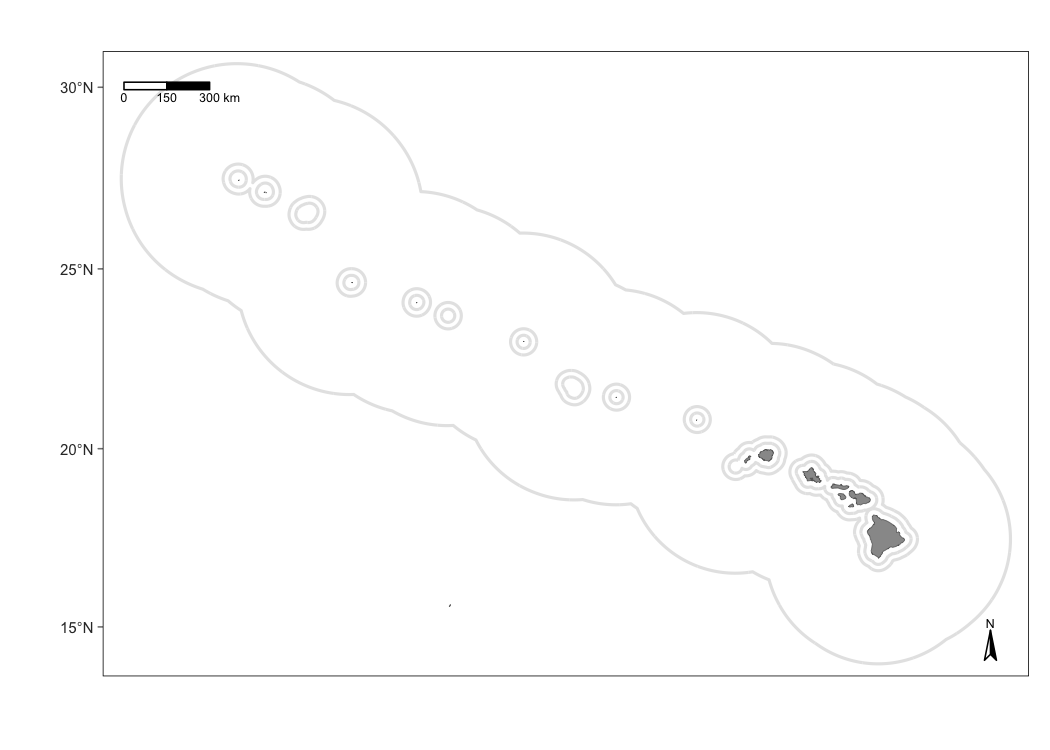
\includegraphics[width=0.95\textwidth,height=\textheight]{img/map_cnp.png}

We also have a base map for the California Current \ldots{}

\begin{Shaded}
\begin{Highlighting}[]
\NormalTok{m <-}\StringTok{ }\KeywordTok{map_base}\NormalTok{(}\DataTypeTok{region=}\StringTok{'ccs'}\NormalTok{)}
\NormalTok{m}
\end{Highlighting}
\end{Shaded}

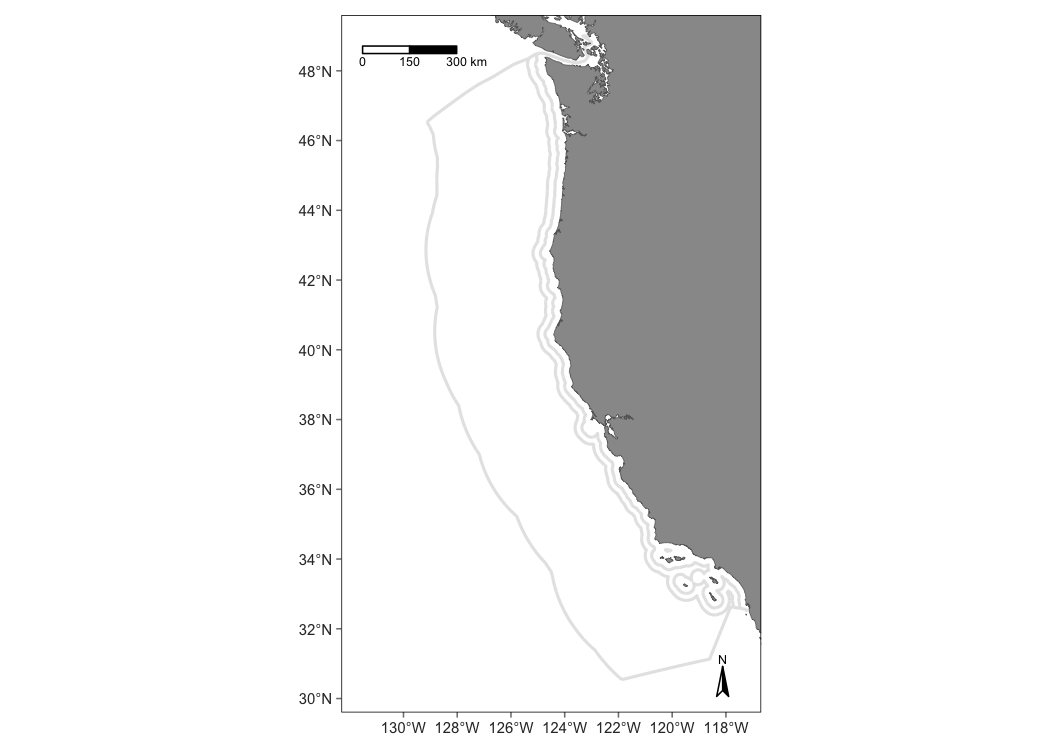
\includegraphics[width=0.95\textwidth,height=\textheight]{img/map_ccs.png}

And the ETP:

\begin{Shaded}
\begin{Highlighting}[]
\NormalTok{m <-}\StringTok{ }\KeywordTok{map_base}\NormalTok{(}\DataTypeTok{region=}\StringTok{'etp'}\NormalTok{)}
\NormalTok{m}
\end{Highlighting}
\end{Shaded}

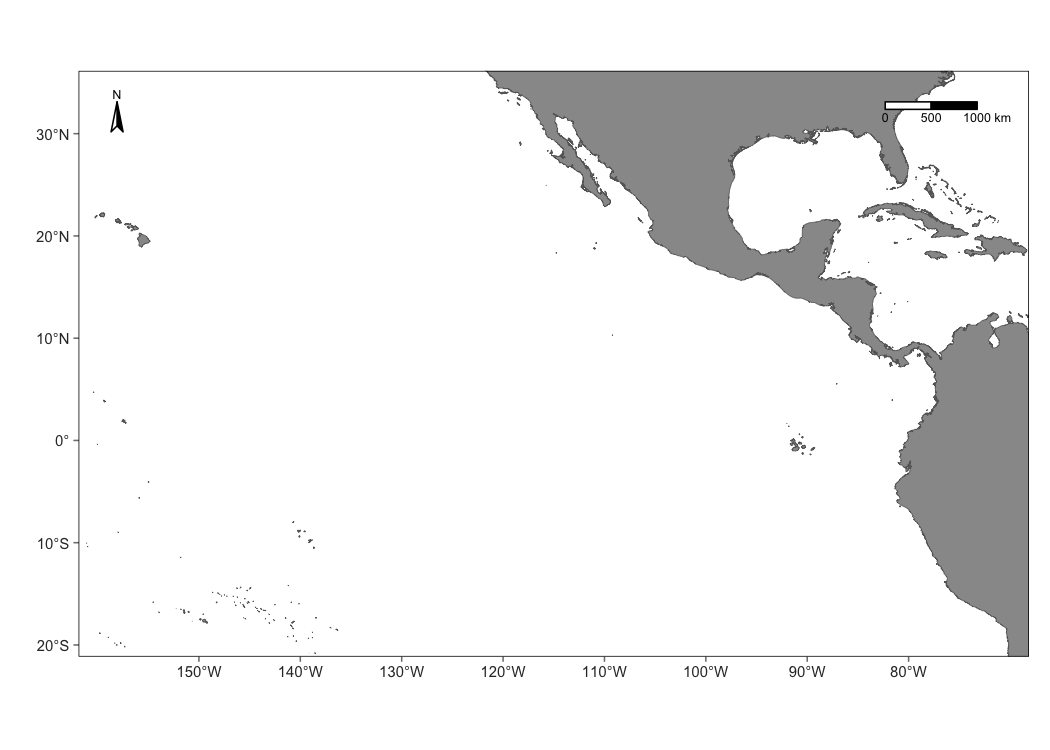
\includegraphics[width=0.95\textwidth,height=\textheight]{img/map_etp.png}

\hypertarget{add-strata}{%
\subsection*{Add strata}\label{add-strata}}
\addcontentsline{toc}{subsection}{Add strata}

Add your research strata to your map:

\begin{Shaded}
\begin{Highlighting}[]
\NormalTok{m <-}\StringTok{ }\KeywordTok{map_base}\NormalTok{(}\DataTypeTok{region=}\StringTok{'cnp'}\NormalTok{)}
\end{Highlighting}
\end{Shaded}

\begin{Shaded}
\begin{Highlighting}[]
\NormalTok{m1 <-}\StringTok{ }\KeywordTok{map_strata}\NormalTok{(m,}
\NormalTok{                cruz_}\DecValTok{1720}\OperatorTok{$}\NormalTok{settings, }
                \DataTypeTok{region=}\StringTok{'cnp'}\NormalTok{)}
\end{Highlighting}
\end{Shaded}

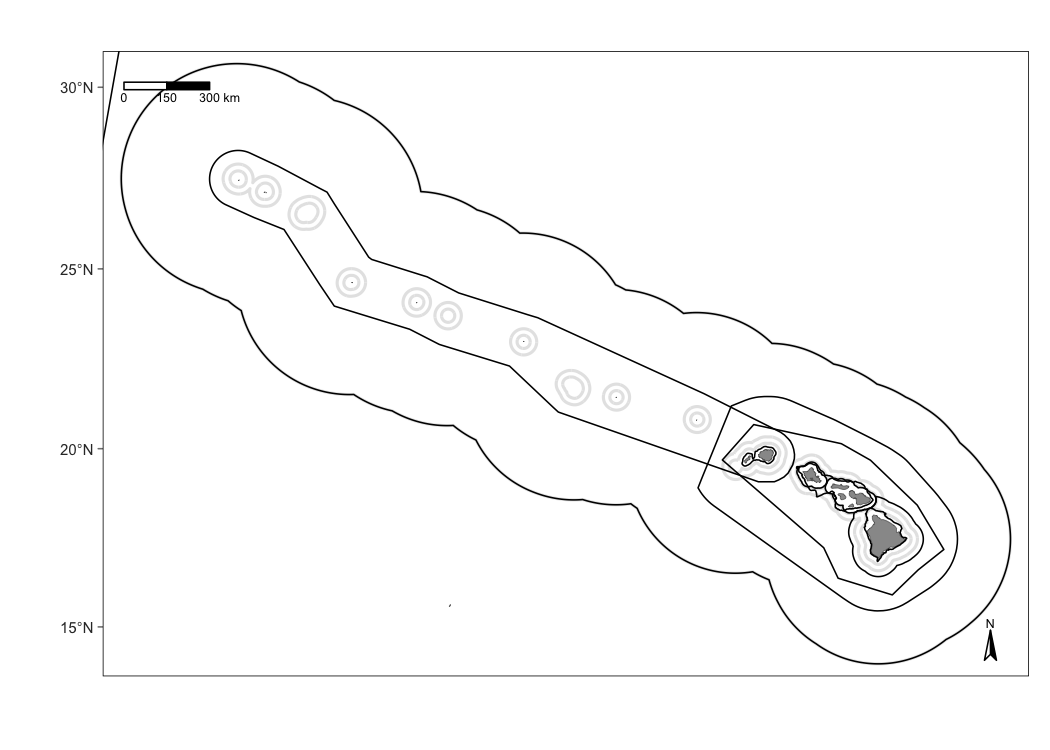
\includegraphics[width=0.95\textwidth,height=\textheight]{img/map_cnp_strata.png}

\hypertarget{add-survey-tracks}{%
\subsection*{Add survey tracks}\label{add-survey-tracks}}
\addcontentsline{toc}{subsection}{Add survey tracks}

\begin{Shaded}
\begin{Highlighting}[]
\NormalTok{m1 <-}\StringTok{ }\KeywordTok{map_effort}\NormalTok{(m, cruz_}\DecValTok{1720}\NormalTok{)}
\NormalTok{m1}
\end{Highlighting}
\end{Shaded}

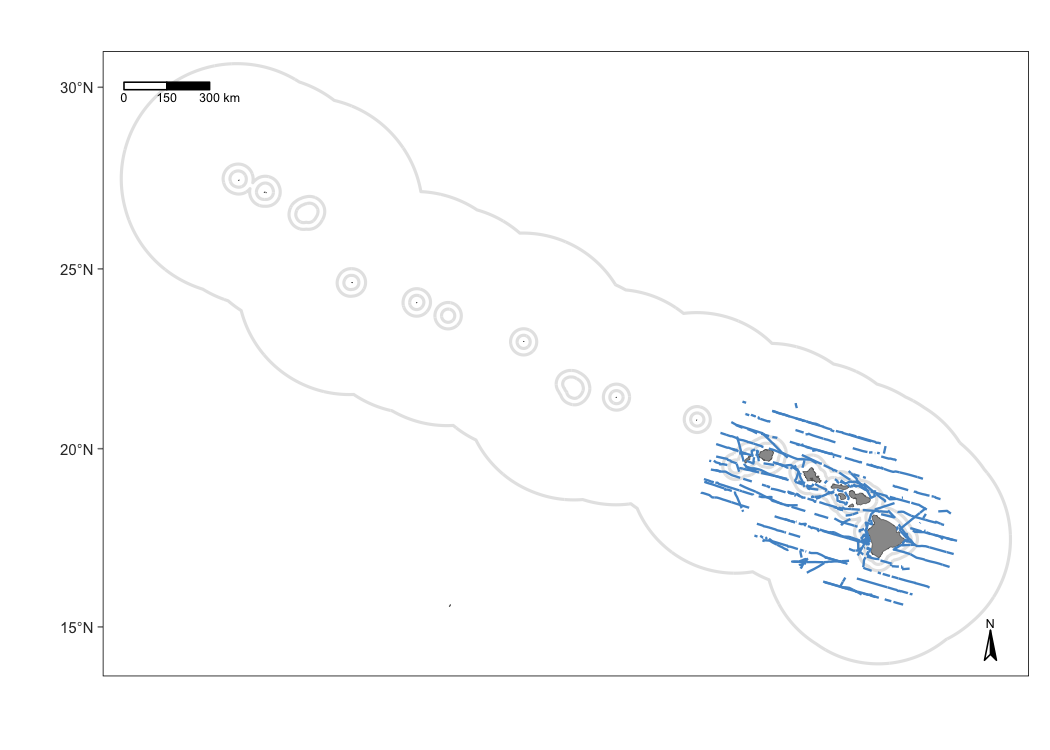
\includegraphics[width=0.95\textwidth,height=\textheight]{img/map_tracks.png}

The defaults of \texttt{map\_effort()} assume, for simplicity, that you want to see the segments to be included in density estimation for the first cohort specified in your settings. You can adjust this and other defaults using the function arguments.

\hypertarget{customizing-effort}{%
\subsubsection*{Customizing effort}\label{customizing-effort}}
\addcontentsline{toc}{subsubsection}{Customizing effort}

\hypertarget{inputs}{%
\paragraph{Inputs}\label{inputs}}
\addcontentsline{toc}{paragraph}{Inputs}

This map changes survey track thickness and color.

\begin{Shaded}
\begin{Highlighting}[]
\NormalTok{m1 <-}\StringTok{ }\KeywordTok{map_effort}\NormalTok{(m, }
\NormalTok{                cruz_}\DecValTok{1720}\NormalTok{,}
                \DataTypeTok{effort_color=}\StringTok{'firebrick'}\NormalTok{,}
                \DataTypeTok{effort_stroke=}\FloatTok{2.5}\NormalTok{,}
                \DataTypeTok{effort_linetype=}\DecValTok{1}\NormalTok{,)}
\end{Highlighting}
\end{Shaded}

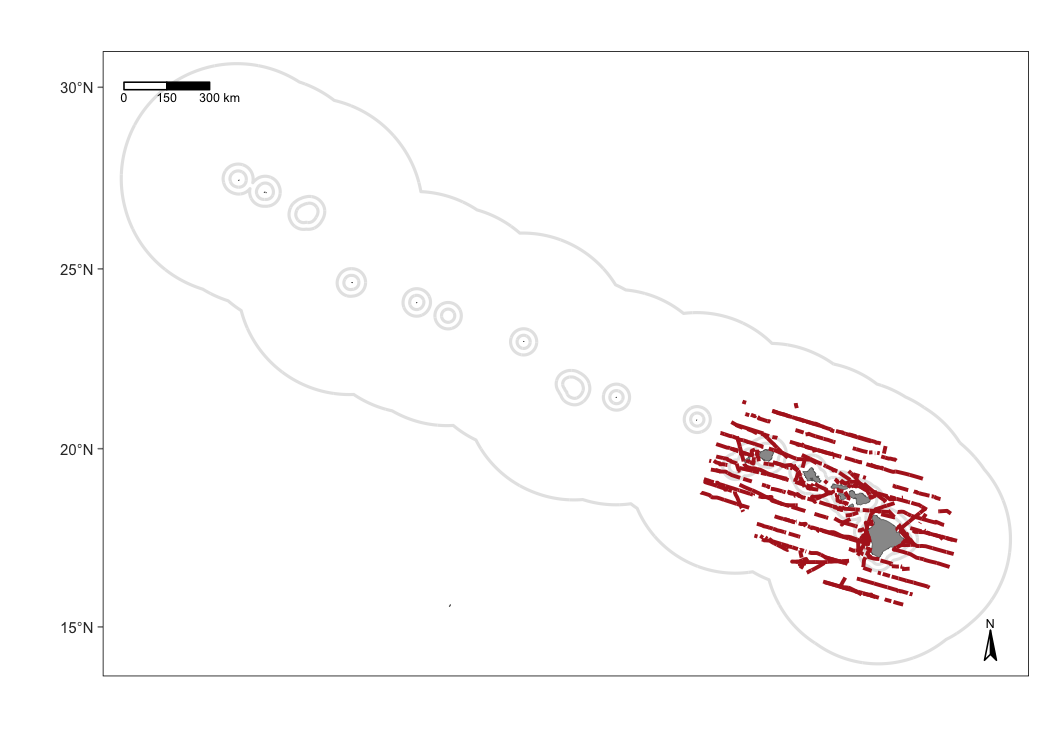
\includegraphics[width=0.95\textwidth,height=\textheight]{img/map_tracks2.png}

\hypertarget{color-code-conditions}{%
\paragraph{Color-code conditions}\label{color-code-conditions}}
\addcontentsline{toc}{paragraph}{Color-code conditions}

Your second customization option is to add format variables to the \texttt{segments} slot of the cohort of interest in the \texttt{cruz} object. This gives you full control of line color, thickness, and line-type according to whatever specifications you wish to set, e.g., color-coding by effort type or Beaufort sea state.

This is possible because the function \texttt{map\_effort()} looks for the variables \texttt{col} (line color), \texttt{lwd} (line thickness or stroke), and \texttt{lty} (line type) in the columns of \texttt{cruz\$segments}. If these columns exist, the values therein will be used instead of the function defaults.

For example, color-code by Beaufort scale:

\begin{Shaded}
\begin{Highlighting}[]
\CommentTok{# Save copy of segments to modify}
\NormalTok{cruzi <-}\StringTok{ }\NormalTok{cruz_}\DecValTok{1720}
\NormalTok{segments <-}\StringTok{ }\NormalTok{cruzi}\OperatorTok{$}\NormalTok{cohorts}\OperatorTok{$}\NormalTok{all}\OperatorTok{$}\NormalTok{segments}

\CommentTok{# Add column `col`: color code by BFT sea state}
\NormalTok{bft_colors <-}\StringTok{ }\KeywordTok{c}\NormalTok{(}\StringTok{'steelblue4'}\NormalTok{,}\StringTok{'steelblue2'}\NormalTok{,}\StringTok{'cadetblue1'}\NormalTok{,}\StringTok{'grey'}\NormalTok{)}
\NormalTok{segments}\OperatorTok{$}\NormalTok{col <-}\StringTok{ }\NormalTok{bft_colors[}\DecValTok{4}\NormalTok{]}
\NormalTok{segments}\OperatorTok{$}\NormalTok{col[ segments}\OperatorTok{$}\NormalTok{avgBft }\OperatorTok{<=}\StringTok{ }\DecValTok{7}\NormalTok{ ] <-}\StringTok{ }\NormalTok{bft_colors[}\DecValTok{3}\NormalTok{] }\CommentTok{# bft 5 +}
\NormalTok{segments}\OperatorTok{$}\NormalTok{col[ segments}\OperatorTok{$}\NormalTok{avgBft }\OperatorTok{<=}\StringTok{ }\DecValTok{4}\NormalTok{ ] <-}\StringTok{ }\NormalTok{bft_colors[}\DecValTok{2}\NormalTok{] }\CommentTok{# bft 3 - 4}
\NormalTok{segments}\OperatorTok{$}\NormalTok{col[ segments}\OperatorTok{$}\NormalTok{avgBft }\OperatorTok{<=}\StringTok{ }\DecValTok{2}\NormalTok{ ] <-}\StringTok{ }\NormalTok{bft_colors[}\DecValTok{1}\NormalTok{] }\CommentTok{# bft 0 -2}

\CommentTok{# Update sub_segments slot in `cruz` object}
\NormalTok{cruzi}\OperatorTok{$}\NormalTok{cohorts}\OperatorTok{$}\NormalTok{all}\OperatorTok{$}\NormalTok{segments <-}\StringTok{ }\NormalTok{segments}

\CommentTok{# Update map }
\NormalTok{m_custom2 <-}\StringTok{ }\KeywordTok{map_effort}\NormalTok{(m, cruzi)}

\CommentTok{# Add legend using native functions from mapping package `tmap`}
\NormalTok{m_custom2 <-}\StringTok{ }
\StringTok{  }\NormalTok{m_custom2 }\OperatorTok{+}\StringTok{ }
\StringTok{  }\NormalTok{tmap}\OperatorTok{::}\KeywordTok{tm_add_legend}\NormalTok{(}\StringTok{'line'}\NormalTok{, }
                        \DataTypeTok{col =}\NormalTok{ bft_colors,}
                        \DataTypeTok{lwd =} \DecValTok{3}\NormalTok{,}
                        \DataTypeTok{labels =} \KeywordTok{c}\NormalTok{(}\StringTok{' 0 - 2'}\NormalTok{, }
                                   \StringTok{' 3 - 4'}\NormalTok{, }
                                   \StringTok{' 5 +'}\NormalTok{, }
                                   \StringTok{' no data'}\NormalTok{),}
                         \DataTypeTok{title=}\StringTok{"Beaufort sea state"}\NormalTok{) }\OperatorTok{+}
\StringTok{  }\NormalTok{tmap}\OperatorTok{::}\KeywordTok{tm_layout}\NormalTok{(}\DataTypeTok{legend.position=}\KeywordTok{c}\NormalTok{(}\StringTok{'left'}\NormalTok{,}\StringTok{'bottom'}\NormalTok{))}

\CommentTok{# Show map}
\NormalTok{m_custom2}
\end{Highlighting}
\end{Shaded}

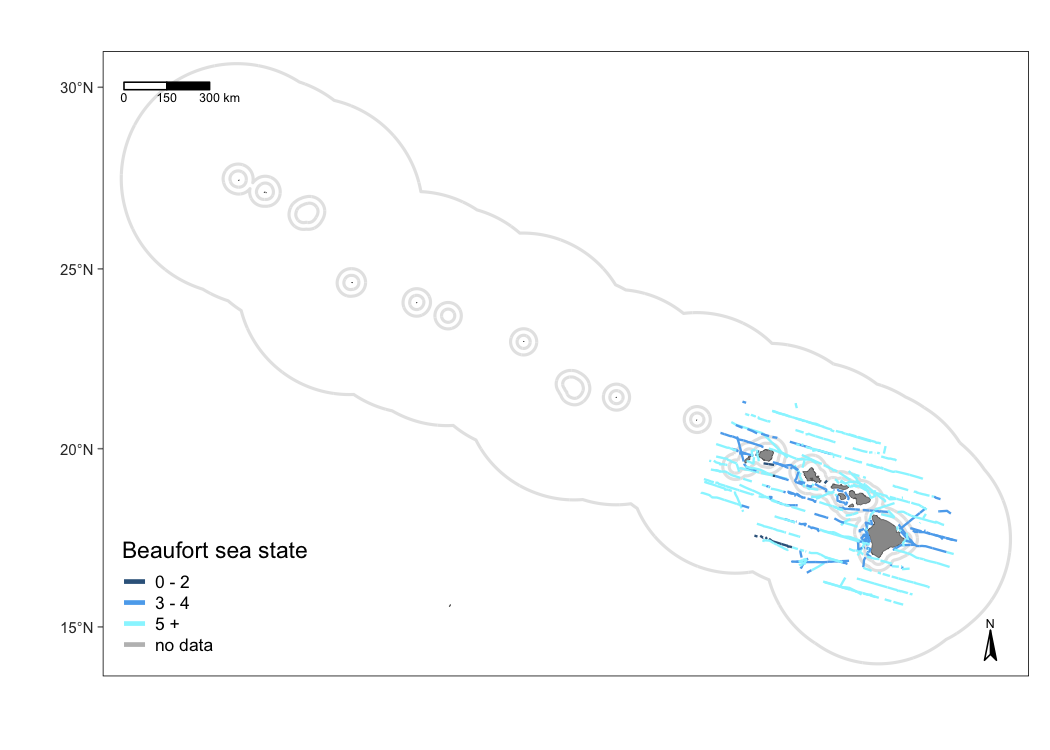
\includegraphics[width=0.95\textwidth,height=\textheight]{img/map_tracks3.png}

\hypertarget{add-sightings}{%
\subsection*{Add sightings}\label{add-sightings}}
\addcontentsline{toc}{subsection}{Add sightings}

Use the function \texttt{map\_sightings()} to add sightings to your map:

\begin{Shaded}
\begin{Highlighting}[]
\NormalTok{m1 <-}\StringTok{ }\KeywordTok{map_sightings}\NormalTok{(m, cruz_}\DecValTok{1720}\NormalTok{)}
\end{Highlighting}
\end{Shaded}

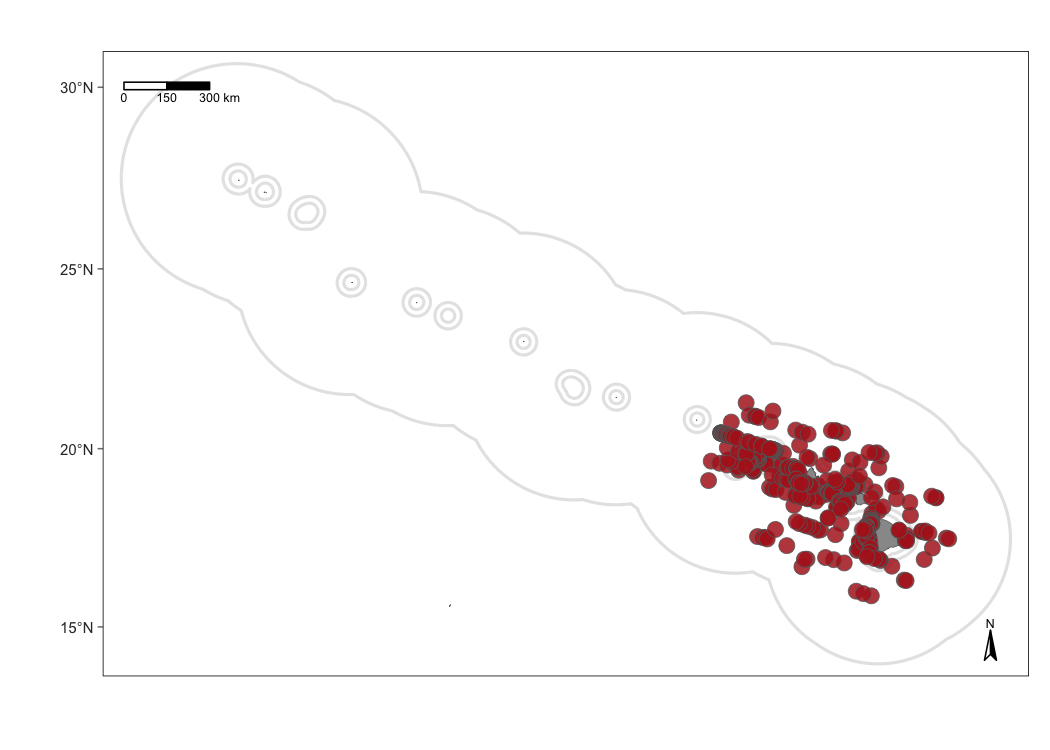
\includegraphics[width=0.95\textwidth,height=\textheight]{img/map_sits.png}

\hypertarget{customizing-sightings}{%
\subsubsection*{Customizing sightings}\label{customizing-sightings}}
\addcontentsline{toc}{subsubsection}{Customizing sightings}

To demonstrate some of the customization options, consider this map that shows sightings of false killer whales with custom dot color, shape, and size:

\begin{Shaded}
\begin{Highlighting}[]
\NormalTok{m1 <-}\StringTok{ }\KeywordTok{map_sightings}\NormalTok{(m,}
\NormalTok{                    cruz_}\DecValTok{1720}\NormalTok{,}
                    \DataTypeTok{include_species =} \StringTok{'033'}\NormalTok{,}
                    \DataTypeTok{color_base =} \StringTok{'purple'}\NormalTok{,}
                    \DataTypeTok{shape_base =} \DecValTok{18}\NormalTok{,}
                    \DataTypeTok{size_base =} \DecValTok{1}\NormalTok{)}
\end{Highlighting}
\end{Shaded}

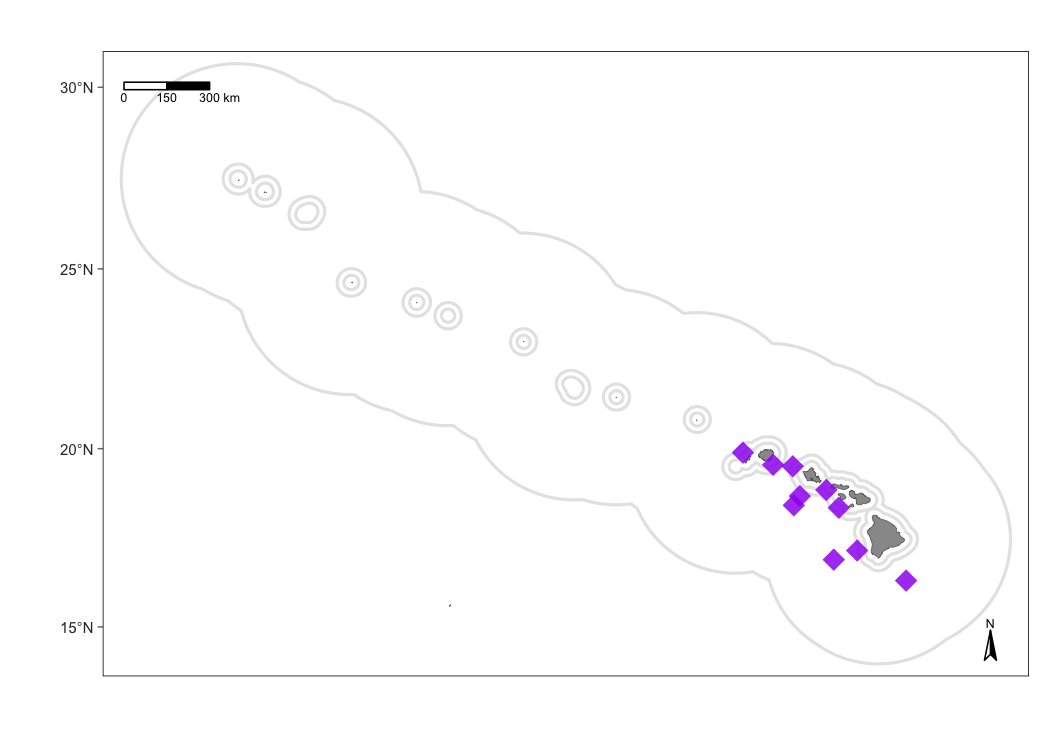
\includegraphics[width=0.95\textwidth,height=\textheight]{img/map_sits2.png}

Next is a map of humpback whales and sperm whales, color-coded by species and shape-coded by whether or not the sighting will be included in the analysis:

\begin{Shaded}
\begin{Highlighting}[]
\NormalTok{m1 <-}\StringTok{ }\KeywordTok{map_sightings}\NormalTok{(m, }
\NormalTok{                   cruz_}\DecValTok{1720}\NormalTok{,}
                   \DataTypeTok{include_species =} \KeywordTok{c}\NormalTok{(}\StringTok{'076'}\NormalTok{,}\StringTok{'046'}\NormalTok{),}
                   \DataTypeTok{color_code =} \OtherTok{TRUE}\NormalTok{,}
                   \DataTypeTok{shape_code =} \OtherTok{TRUE}\NormalTok{)}
\end{Highlighting}
\end{Shaded}

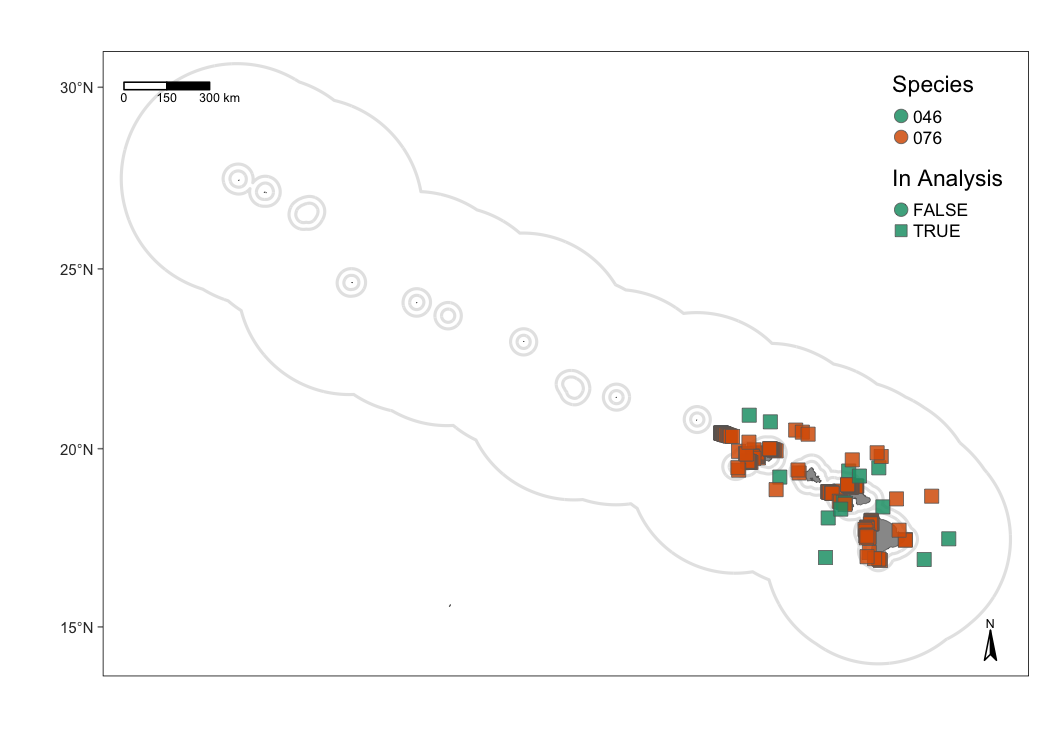
\includegraphics[width=0.95\textwidth,height=\textheight]{img/map_sits3.png}

\hypertarget{overview-1}{%
\subsection*{Overview}\label{overview-1}}
\addcontentsline{toc}{subsection}{Overview}

Here is an overview of the steps needed to map strata, survey tracks, and sightings all together:

\begin{Shaded}
\begin{Highlighting}[]
\NormalTok{m <-}\StringTok{ }\KeywordTok{map_base}\NormalTok{(}\StringTok{'cnp'}\NormalTok{) }
\NormalTok{m <-}\StringTok{ }\KeywordTok{map_strata}\NormalTok{(m, cruz_}\DecValTok{1720}\OperatorTok{$}\NormalTok{settings)}
\NormalTok{m <-}\StringTok{ }\KeywordTok{map_effort}\NormalTok{(m, cruz_}\DecValTok{1720}\NormalTok{)}
\NormalTok{m <-}\StringTok{ }\KeywordTok{map_sightings}\NormalTok{(m, cruz_}\DecValTok{1720}\NormalTok{, }\DataTypeTok{size_base=}\NormalTok{.}\DecValTok{4}\NormalTok{)}
\NormalTok{m }
\end{Highlighting}
\end{Shaded}

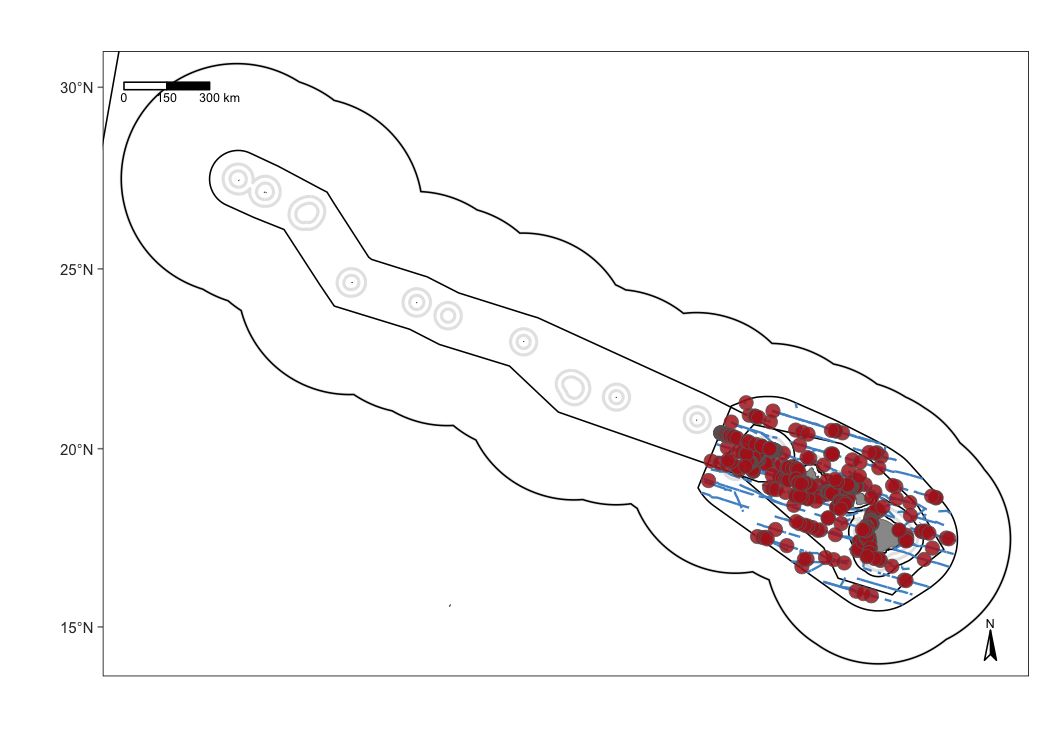
\includegraphics[width=0.95\textwidth,height=\textheight]{img/map_overview.png}

\hypertarget{interactive-maps}{%
\section*{Interactive maps}\label{interactive-maps}}
\addcontentsline{toc}{section}{Interactive maps}

\texttt{LTabundR} also has an interactive map function, which maps survey data using the \texttt{leaflet} package.

\begin{Shaded}
\begin{Highlighting}[]
 \KeywordTok{map_cruz}\NormalTok{(cruz_}\DecValTok{1720}\NormalTok{,}
          \DataTypeTok{cohort=}\DecValTok{1}\NormalTok{,}
          \DataTypeTok{eez_show=}\OtherTok{FALSE}\NormalTok{,}
          \DataTypeTok{strata_show=}\OtherTok{FALSE}\NormalTok{,}
          \DataTypeTok{effort_show=}\OtherTok{TRUE}\NormalTok{,}
          \DataTypeTok{effort_resolution=}\DecValTok{1}\NormalTok{,}
          \DataTypeTok{sightings_show=}\OtherTok{TRUE}\NormalTok{,}
          \DataTypeTok{sightings_color =} \StringTok{'firebrick'}\NormalTok{,}
          \DataTypeTok{verbose=}\OtherTok{FALSE}\NormalTok{)}
\end{Highlighting}
\end{Shaded}

Note that you can also click on sightings and tracklines to see their details. Refer to the documentation for this function (\texttt{?map\_cruz}) to see all the options available for stylizing these maps.

\hypertarget{interactive-dashboard}{%
\section*{Interactive dashboard}\label{interactive-dashboard}}
\addcontentsline{toc}{section}{Interactive dashboard}

Finally, note that \texttt{LTabundR} comes with an interactive data explorer app (a \texttt{Shiny} app) for filtering survey data according to effort scenario and species code, toggling \texttt{map\_cruz()} settings, and reviewing summary tables of effort and sightings (including inspection of truncation distances).

\begin{Shaded}
\begin{Highlighting}[]
\KeywordTok{cruz_explorer}\NormalTok{(cruz)}
\end{Highlighting}
\end{Shaded}

\emph{Screenshots from this app:}

~\\

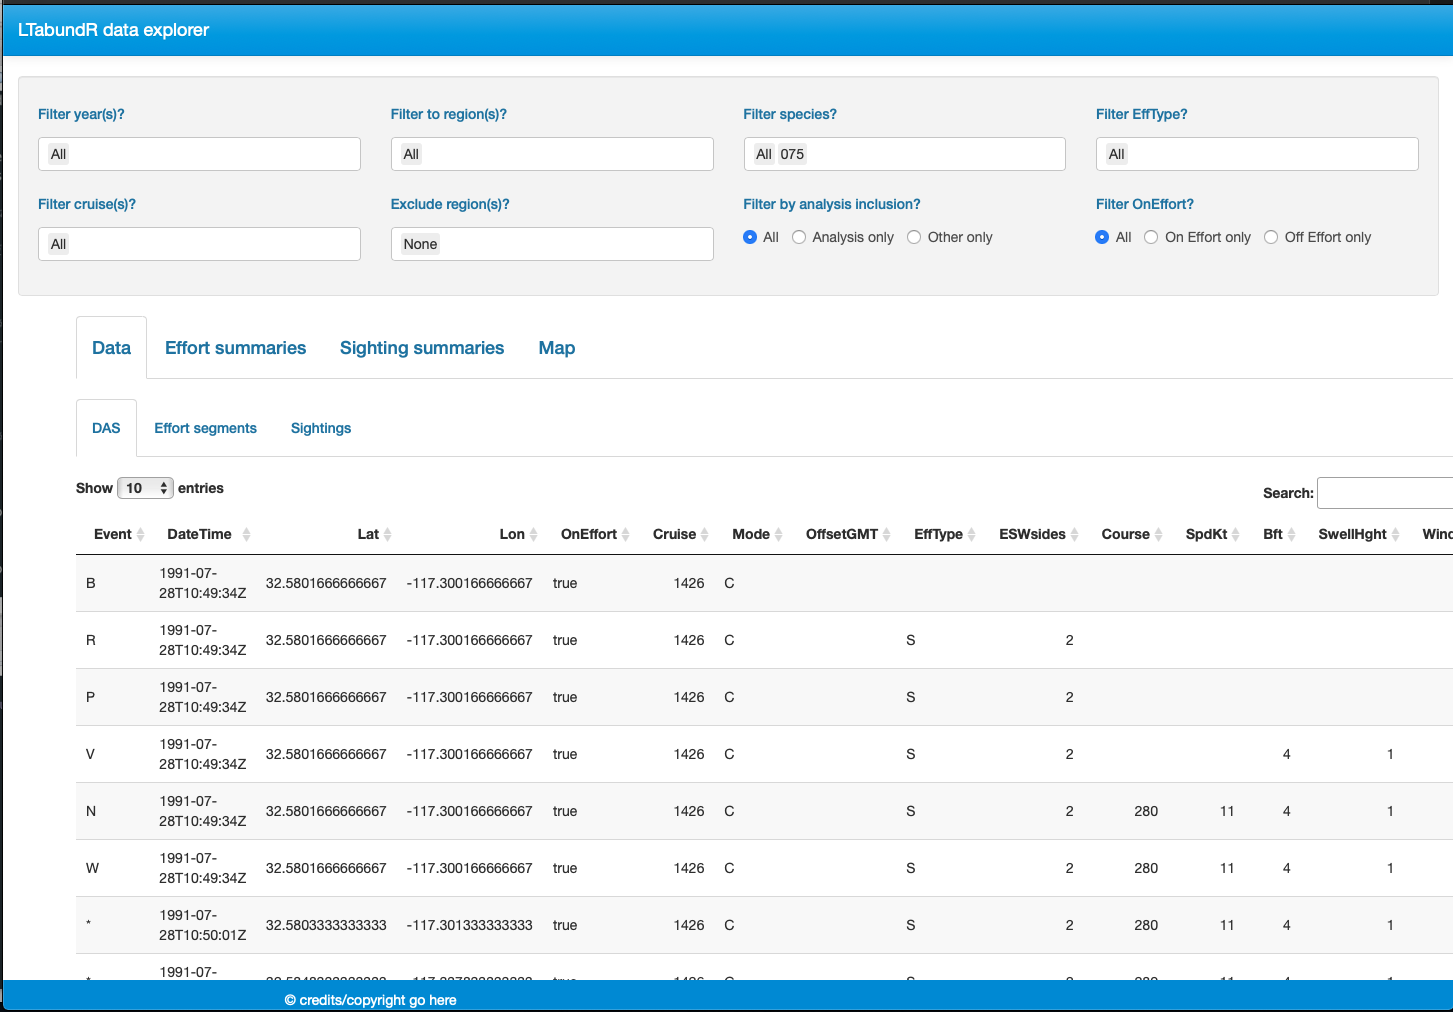
\includegraphics[width=0.85\textwidth,height=\textheight]{img/app-1.png}
~\\
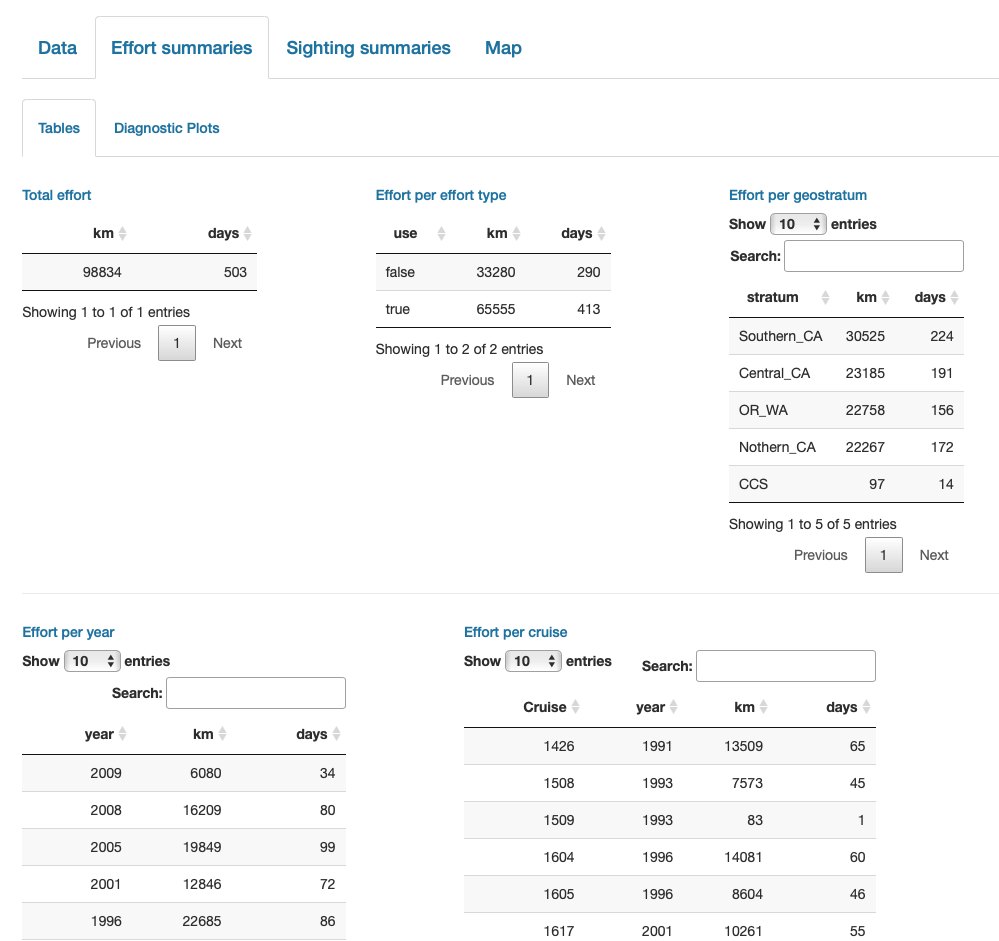
\includegraphics[width=0.85\textwidth,height=\textheight]{img/app-2.png}
~\\
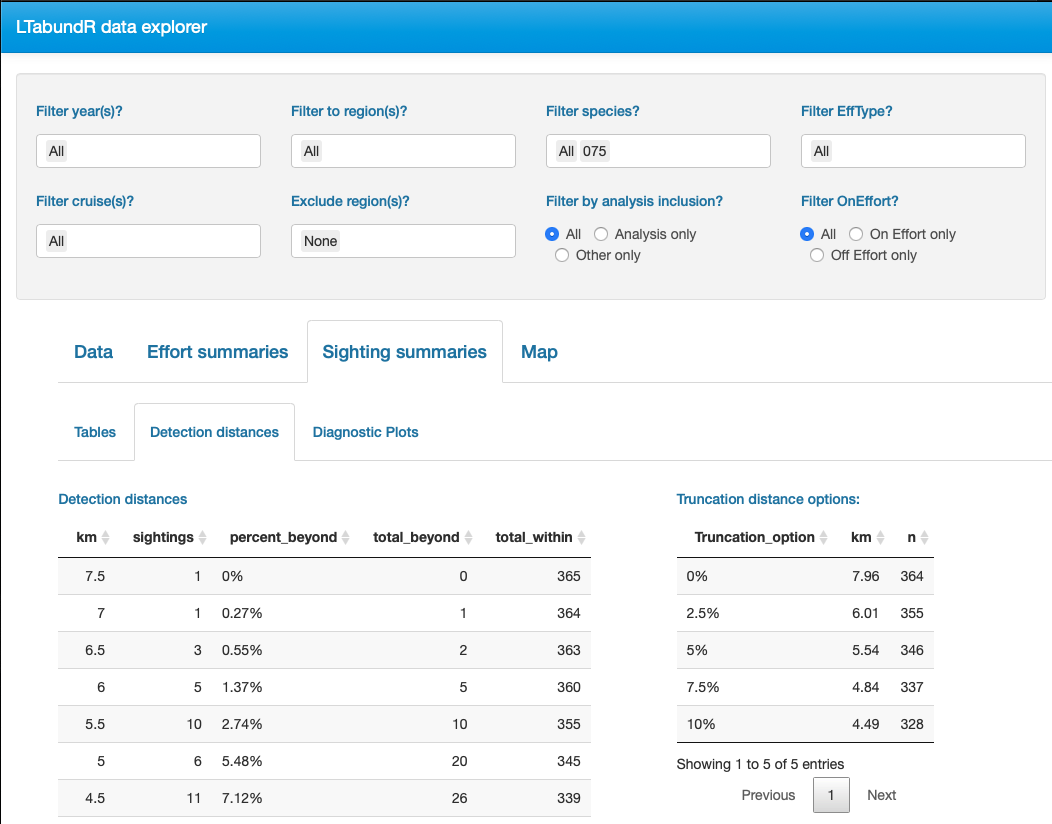
\includegraphics[width=0.85\textwidth,height=\textheight]{img/app-3.png}
~\\
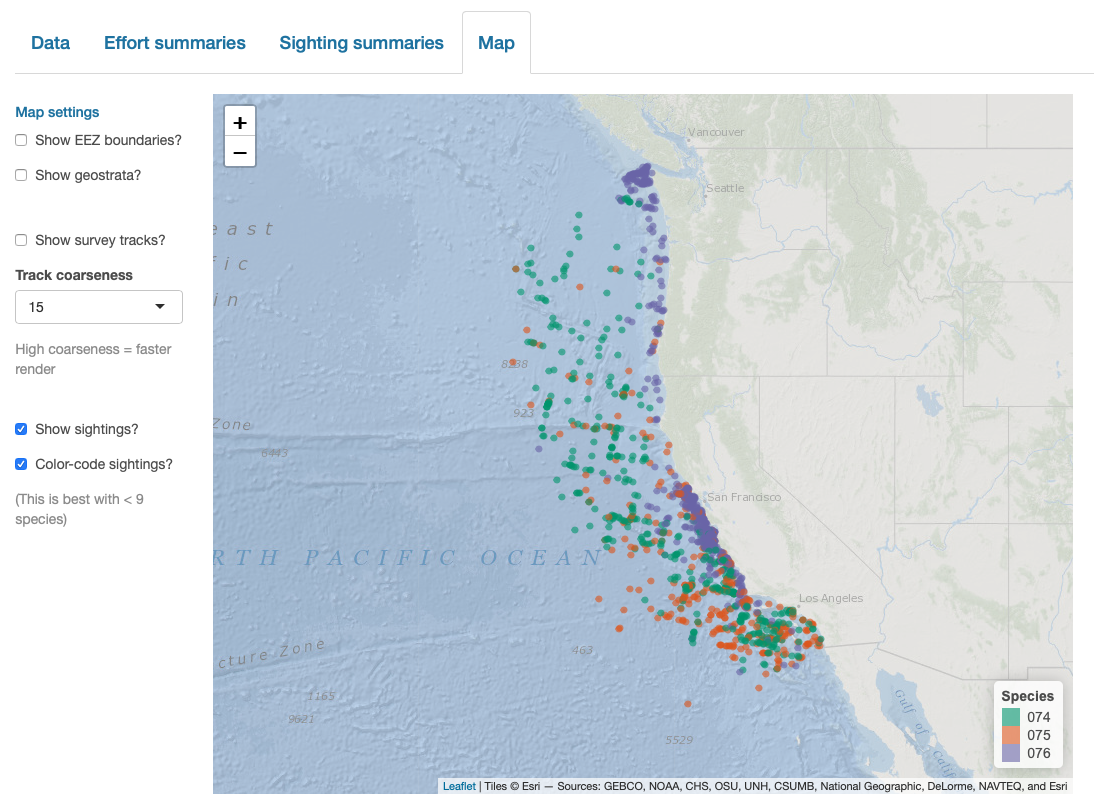
\includegraphics[width=0.85\textwidth,height=\textheight]{img/app-4.png}
~\\
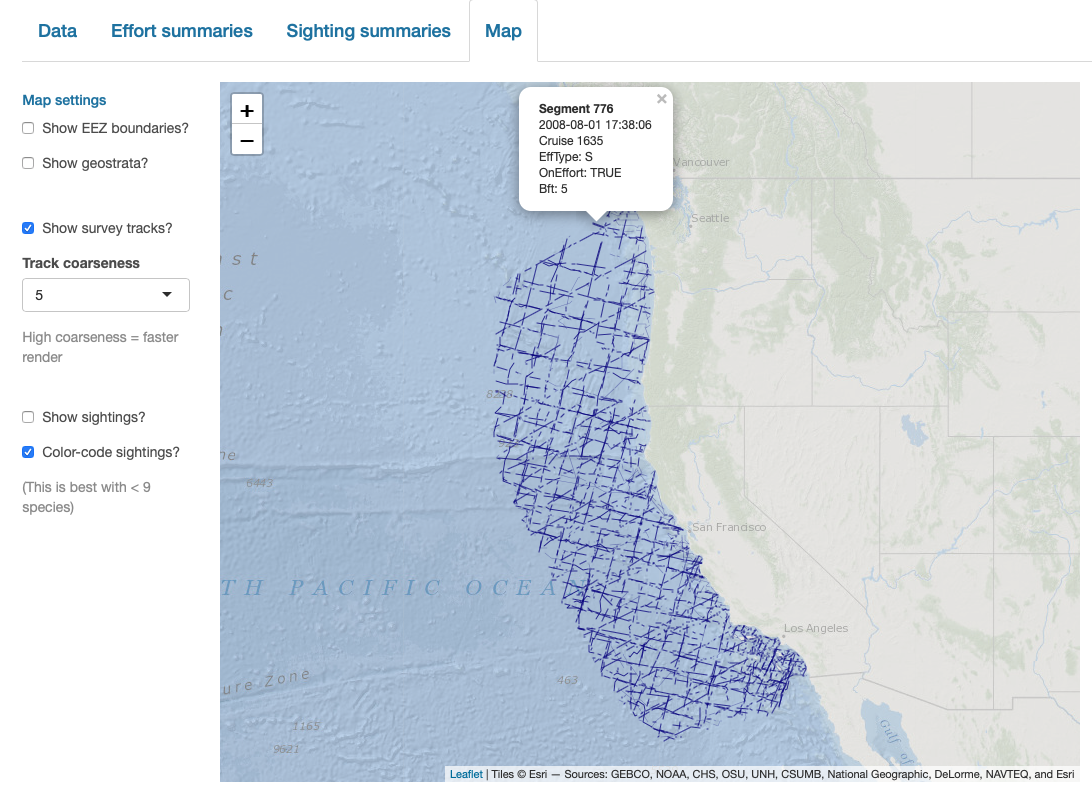
\includegraphics[width=0.85\textwidth,height=\textheight]{img/app-5.png}

\hypertarget{filter}{%
\chapter{Filter \& combine surveys}\label{filter}}

You may soon encounter the need to filter a processed \texttt{cruz} object to only certain years, regions, or cruise numbers. You may also need to combine one processed \texttt{cruz} object with another.

Here we will continue with the \texttt{cruz} object we created on the previous page. As a reminder, here is the data structure of that object:

\begin{Shaded}
\begin{Highlighting}[]
\KeywordTok{cruz_structure}\NormalTok{(cruz)}
\StringTok{"cruz"}\NormalTok{ list structure }\OperatorTok{==}\ErrorTok{======================}

\ErrorTok{$}\NormalTok{settings}
         \OperatorTok{$}\NormalTok{strata }\OperatorTok{---}\StringTok{ }\NormalTok{with }\DecValTok{11}\NormalTok{ polygon coordinate sets}
         \OperatorTok{$}\NormalTok{survey }\OperatorTok{---}\StringTok{ }\NormalTok{with }\DecValTok{10}\NormalTok{ input arguments}
         \OperatorTok{$}\NormalTok{cohorts }\OperatorTok{---}\StringTok{ }\NormalTok{with }\DecValTok{3}\NormalTok{ cohorts specified, each with }\DecValTok{19}\NormalTok{ input arguments}

\OperatorTok{$}\NormalTok{strata}
\NormalTok{       ... containing a summary dataframe of }\DecValTok{11}\NormalTok{ geostrata and their spatial areas}
\NormalTok{       ... geostratum names}\OperatorTok{:}
\StringTok{           }\NormalTok{HI_EEZ, OtherCNP, MHI, WHICEAS, Spotted_OU, Spotted_FI, Spotted_BI, Bottlenose_KaNi, Bottlenose_OUFI, Bottlenose_BI, NWHI}

\OperatorTok{$}\NormalTok{cohorts}

        \OperatorTok{$}\NormalTok{all}
\NormalTok{            geostrata}\OperatorTok{:}\StringTok{ }\NormalTok{WHICEAS, HI_EEZ, OtherCNP}
            \OperatorTok{$}\NormalTok{segments  }\OperatorTok{---}\StringTok{ }\NormalTok{with }\DecValTok{1888} \KeywordTok{segments}\NormalTok{ (}\DataTypeTok{median =} \FloatTok{149.3}\NormalTok{ km)}
            \OperatorTok{$}\NormalTok{das       }\OperatorTok{---}\StringTok{ }\NormalTok{with }\DecValTok{329609}\NormalTok{ data rows}
            \OperatorTok{$}\NormalTok{sightings }\OperatorTok{---}\StringTok{ }\NormalTok{with }\DecValTok{3932}\NormalTok{ detections}
            \OperatorTok{$}\NormalTok{subgroups }\OperatorTok{---}\StringTok{ }\NormalTok{with }\DecValTok{255}\NormalTok{ subgroups, }\DecValTok{49}\NormalTok{ sightings, and }\DecValTok{389}\NormalTok{ events}

        \OperatorTok{$}\NormalTok{bottlenose}
\NormalTok{            geostrata}\OperatorTok{:}\StringTok{ }\NormalTok{WHICEAS, HI_EEZ, OtherCNP, Bottlenose_BI, Bottlenose_OUFI, Bottlenose_KaNi}
            \OperatorTok{$}\NormalTok{segments  }\OperatorTok{---}\StringTok{ }\NormalTok{with }\DecValTok{2049} \KeywordTok{segments}\NormalTok{ (}\DataTypeTok{median =} \FloatTok{148.8}\NormalTok{ km)}
            \OperatorTok{$}\NormalTok{das       }\OperatorTok{---}\StringTok{ }\NormalTok{with }\DecValTok{329609}\NormalTok{ data rows}
            \OperatorTok{$}\NormalTok{sightings }\OperatorTok{---}\StringTok{ }\NormalTok{with }\DecValTok{522}\NormalTok{ detections}

        \OperatorTok{$}\NormalTok{spotted}
\NormalTok{            geostrata}\OperatorTok{:}\StringTok{ }\NormalTok{WHICEAS, HI_EEZ, OtherCNP, Spotted_OU, Spotted_FI, Spotted_BI}
            \OperatorTok{$}\NormalTok{segments  }\OperatorTok{---}\StringTok{ }\NormalTok{with }\DecValTok{2053} \KeywordTok{segments}\NormalTok{ (}\DataTypeTok{median =} \FloatTok{148.5}\NormalTok{ km)}
            \OperatorTok{$}\NormalTok{das       }\OperatorTok{---}\StringTok{ }\NormalTok{with }\DecValTok{329609}\NormalTok{ data rows}
            \OperatorTok{$}\NormalTok{sightings }\OperatorTok{---}\StringTok{ }\NormalTok{with }\DecValTok{527}\NormalTok{ detections}
\end{Highlighting}
\end{Shaded}

\hypertarget{filter-1}{%
\section*{Filter}\label{filter-1}}
\addcontentsline{toc}{section}{Filter}

\texttt{LTabundR} lets you filter a \texttt{cruz} object using the function \texttt{filter\_cruz()}.

For example, in our WHICEAS case study, we processed surveys from 1986 - 2020, which we needed to do to model our detection functions, but our interest for mapping is specifically valid effort in 2017 and 2020 only, and only within the \texttt{"WHICEAS"} geostratum.

\begin{Shaded}
\begin{Highlighting}[]
\NormalTok{cruz_}\DecValTok{1720}\NormalTok{ <-}\StringTok{ }
\StringTok{  }\KeywordTok{filter_cruz}\NormalTok{(cruz,}
              \DataTypeTok{analysis_only =} \OtherTok{TRUE}\NormalTok{,}
              \DataTypeTok{years =} \KeywordTok{c}\NormalTok{(}\DecValTok{2017}\NormalTok{, }\DecValTok{2020}\NormalTok{),}
              \DataTypeTok{regions =} \StringTok{'WHICEAS'}\NormalTok{)}
\end{Highlighting}
\end{Shaded}

We will use this filtered \texttt{cruz} object for mapping \& sightings summaries downstream.

\begin{Shaded}
\begin{Highlighting}[]
\KeywordTok{save}\NormalTok{(cruz_}\DecValTok{1720}\NormalTok{,}\DataTypeTok{file=}\StringTok{'whiceas_cruz_1720.RData'}\NormalTok{)}
\end{Highlighting}
\end{Shaded}

Note that \texttt{filter\_cruz()} has many other filter options. See \texttt{?filter\_cruz()} for details.

\hypertarget{combine}{%
\section*{Combine}\label{combine}}
\addcontentsline{toc}{section}{Combine}

Say you have two processed \texttt{cruz} objects: one containing survey effort from the WHICEAS geostratum area only, and one containing survey effort from the pelagic Hawaiian EEZ geostratum (\texttt{"HI\_EEZ"}) that does \emph{not} include WHICEAS effort.

Let's make those fake datasets right now, using \texttt{filter\_cruz()}:

\textbf{WHICEAS-only data:}

\begin{Shaded}
\begin{Highlighting}[]
\NormalTok{cruz_whiceas <-}\StringTok{ }\KeywordTok{filter_cruz}\NormalTok{(cruz, }
                            \DataTypeTok{regions =} \StringTok{'WHICEAS'}\NormalTok{, }
                            \DataTypeTok{verbose =} \OtherTok{FALSE}\NormalTok{)}
\end{Highlighting}
\end{Shaded}

\textbf{Pelagic Hawaiian EEZ - only data:}

\begin{Shaded}
\begin{Highlighting}[]
\NormalTok{cruz_hi_eez <-}\StringTok{ }\KeywordTok{filter_cruz}\NormalTok{(cruz, }
                           \DataTypeTok{regions =} \StringTok{'HI_EEZ'}\NormalTok{, }
                           \DataTypeTok{not_regions =} \StringTok{'WHICEAS'}\NormalTok{, }
                           \DataTypeTok{verbose =} \OtherTok{FALSE}\NormalTok{)}
\end{Highlighting}
\end{Shaded}

Say you want to combine these datasets together in order to reconstruct the equivalent of our original \texttt{cruz} object. You can do this with the \texttt{LTabundR} function, \texttt{cruz\_combine()}.

\begin{Shaded}
\begin{Highlighting}[]
\CommentTok{# Make a list of cruz objects}
\NormalTok{cruzes <-}\StringTok{ }\KeywordTok{list}\NormalTok{(cruz_whiceas, cruz_hi_eez)}

\CommentTok{# Now combine}
\NormalTok{cruz_demo <-}\StringTok{ }\KeywordTok{cruz_combine}\NormalTok{(cruzes)}
\end{Highlighting}
\end{Shaded}

Re-constituted data structure:

\begin{Shaded}
\begin{Highlighting}[]
\KeywordTok{cruz_structure}\NormalTok{(cruz_demo)}
\StringTok{"cruz"}\NormalTok{ list structure }\OperatorTok{==}\ErrorTok{======================}

\ErrorTok{$}\NormalTok{settings}
         \OperatorTok{$}\NormalTok{strata }\OperatorTok{---}\StringTok{ }\NormalTok{with }\DecValTok{11}\NormalTok{ polygon coordinate sets}
         \OperatorTok{$}\NormalTok{survey }\OperatorTok{---}\StringTok{ }\NormalTok{with }\DecValTok{10}\NormalTok{ input arguments}
         \OperatorTok{$}\NormalTok{cohorts }\OperatorTok{---}\StringTok{ }\NormalTok{with }\DecValTok{3}\NormalTok{ cohorts specified, each with }\DecValTok{19}\NormalTok{ input arguments}

\OperatorTok{$}\NormalTok{strata}
\NormalTok{       ... containing a summary dataframe of }\DecValTok{11}\NormalTok{ geostrata and their spatial areas}
\NormalTok{       ... geostratum names}\OperatorTok{:}
\StringTok{           }\NormalTok{HI_EEZ, OtherCNP, MHI, WHICEAS, Spotted_OU, Spotted_FI, Spotted_BI, Bottlenose_KaNi, Bottlenose_OUFI, Bottlenose_BI, NWHI}

\OperatorTok{$}\NormalTok{cohorts}

        \OperatorTok{$}\NormalTok{all}
\NormalTok{            geostrata}\OperatorTok{:}\StringTok{ }\NormalTok{WHICEAS, HI_EEZ, OtherCNP}
            \OperatorTok{$}\NormalTok{segments  }\OperatorTok{---}\StringTok{ }\NormalTok{with }\DecValTok{1013} \KeywordTok{segments}\NormalTok{ (}\DataTypeTok{median =} \FloatTok{149.1}\NormalTok{ km)}
            \OperatorTok{$}\NormalTok{das       }\OperatorTok{---}\StringTok{ }\NormalTok{with }\DecValTok{203387}\NormalTok{ data rows}
            \OperatorTok{$}\NormalTok{sightings }\OperatorTok{---}\StringTok{ }\NormalTok{with }\DecValTok{1793}\NormalTok{ detections}
            \OperatorTok{$}\NormalTok{subgroups }\OperatorTok{---}\StringTok{ }\NormalTok{with }\DecValTok{146}\NormalTok{ subgroups, }\DecValTok{21}\NormalTok{ sightings, and }\DecValTok{212}\NormalTok{ events}

        \OperatorTok{$}\NormalTok{bottlenose}
\NormalTok{            geostrata}\OperatorTok{:}\StringTok{ }\NormalTok{WHICEAS, HI_EEZ, OtherCNP, Bottlenose_BI, Bottlenose_OUFI, Bottlenose_KaNi}
            \OperatorTok{$}\NormalTok{segments  }\OperatorTok{---}\StringTok{ }\NormalTok{with }\DecValTok{1174} \KeywordTok{segments}\NormalTok{ (}\DataTypeTok{median =} \FloatTok{128.3}\NormalTok{ km)}
            \OperatorTok{$}\NormalTok{das       }\OperatorTok{---}\StringTok{ }\NormalTok{with }\DecValTok{203387}\NormalTok{ data rows}
            \OperatorTok{$}\NormalTok{sightings }\OperatorTok{---}\StringTok{ }\NormalTok{with }\DecValTok{277}\NormalTok{ detections}

        \OperatorTok{$}\NormalTok{spotted}
\NormalTok{            geostrata}\OperatorTok{:}\StringTok{ }\NormalTok{WHICEAS, HI_EEZ, OtherCNP, Spotted_OU, Spotted_FI, Spotted_BI}
            \OperatorTok{$}\NormalTok{segments  }\OperatorTok{---}\StringTok{ }\NormalTok{with }\DecValTok{1178} \KeywordTok{segments}\NormalTok{ (}\DataTypeTok{median =} \FloatTok{113.3}\NormalTok{ km)}
            \OperatorTok{$}\NormalTok{das       }\OperatorTok{---}\StringTok{ }\NormalTok{with }\DecValTok{203387}\NormalTok{ data rows}
            \OperatorTok{$}\NormalTok{sightings }\OperatorTok{---}\StringTok{ }\NormalTok{with }\DecValTok{115}\NormalTok{ detections}
\end{Highlighting}
\end{Shaded}

\hypertarget{summarize}{%
\chapter{Summarize survey}\label{summarize}}

Here we will summarize the 2017 \& 2020 survey data we prepared on the previous page.

\begin{Shaded}
\begin{Highlighting}[]
\KeywordTok{load}\NormalTok{(}\StringTok{'whiceas_cruz_1720.RData'}\NormalTok{)}
\end{Highlighting}
\end{Shaded}

\hypertarget{summarize-effort}{%
\section*{Summarize effort}\label{summarize-effort}}
\addcontentsline{toc}{section}{Summarize effort}

The \texttt{summarize\_effort()} functions builds tables with total kilometers and days surveyed.

\begin{Shaded}
\begin{Highlighting}[]
\NormalTok{effort <-}\StringTok{ }\KeywordTok{summarize_effort}\NormalTok{(cruz_}\DecValTok{1720}\NormalTok{,}
                           \DataTypeTok{cohort=}\DecValTok{1}\NormalTok{)}
\end{Highlighting}
\end{Shaded}

This function summarizes effort in several default tables:

\begin{Shaded}
\begin{Highlighting}[]
\NormalTok{effort }\OperatorTok\StringTok{  }\KeywordTok{names}\NormalTok{()}
\NormalTok{[}\DecValTok{1}\NormalTok{] }\StringTok{"total"}            \StringTok{"total_by_cruise"}  \StringTok{"total_by_year"}    \StringTok{"total_by_effort"} 
\NormalTok{[}\DecValTok{5}\NormalTok{] }\StringTok{"total_by_stratum"}
\end{Highlighting}
\end{Shaded}

\hypertarget{total-surveyed}{%
\subsubsection*{Total surveyed}\label{total-surveyed}}
\addcontentsline{toc}{subsubsection}{Total surveyed}

The slot \texttt{\$total} provides the grand total distance and unique dates surveyed:

\begin{Shaded}
\begin{Highlighting}[]
\KeywordTok{library}\NormalTok{(DT)}

\NormalTok{effort}\OperatorTok{$}\NormalTok{total }\OperatorTok\StringTok{ }
\StringTok{  }\NormalTok{DT}\OperatorTok{::}\KeywordTok{datatable}\NormalTok{(}\DataTypeTok{options=}\KeywordTok{list}\NormalTok{(}\DataTypeTok{initComplete =}\NormalTok{ htmlwidgets}\OperatorTok{::}\KeywordTok{JS}\NormalTok{(}
          \StringTok{"function(settings, json) \{$(this.api().table().container()).css(\{'font-size': '9pt'\});\}"}\NormalTok{)}
\NormalTok{       )) }
\end{Highlighting}
\end{Shaded}

\hypertarget{total-surveyed-by-effort}{%
\subsubsection*{Total surveyed by effort}\label{total-surveyed-by-effort}}
\addcontentsline{toc}{subsubsection}{Total surveyed by effort}

The slot \texttt{\$total\_by\_effort} provides the total distance and days surveyed, grouped by segments that will be included in the analysis and those that won't:

\hypertarget{total-surveyed-by-stratum}{%
\subsubsection*{Total surveyed by stratum}\label{total-surveyed-by-stratum}}
\addcontentsline{toc}{subsubsection}{Total surveyed by stratum}

The slot \texttt{\$total\_by\_stratum} provides the total distance and days surveyed within each stratum, again grouped by segments that will be included in the analysis and those that won't:

\hypertarget{summarize-by-beaufort}{%
\section*{Summarize by Beaufort}\label{summarize-by-beaufort}}
\addcontentsline{toc}{section}{Summarize by Beaufort}

\begin{Shaded}
\begin{Highlighting}[]
\NormalTok{bft <-}\StringTok{ }\KeywordTok{summarize_bft}\NormalTok{(cruz_}\DecValTok{1720}\NormalTok{, }\DataTypeTok{cohort=}\DecValTok{1}\NormalTok{)}
\end{Highlighting}
\end{Shaded}

This function summarizes effort by Beaufort in four default tables:

\begin{Shaded}
\begin{Highlighting}[]
\NormalTok{bft }\OperatorTok\StringTok{  }\KeywordTok{names}\NormalTok{()}
\NormalTok{[}\DecValTok{1}\NormalTok{] }\StringTok{"overall"}    \StringTok{"by_year"}    \StringTok{"by_stratum"} \StringTok{"details"}   
\end{Highlighting}
\end{Shaded}

\hypertarget{simple-overall-breakdown}{%
\subsection*{Simple overall breakdown}\label{simple-overall-breakdown}}
\addcontentsline{toc}{subsection}{Simple overall breakdown}

The slot \texttt{\$overall} provides the total effort -- and proportion of effort -- occurring in each Beaufort state:

\hypertarget{breakdown-by-year}{%
\subsection*{Breakdown by year}\label{breakdown-by-year}}
\addcontentsline{toc}{subsection}{Breakdown by year}

The slot \texttt{\$by\_year} provides the above for each year separately:

\hypertarget{breakdown-by-stratum}{%
\subsection*{Breakdown by stratum}\label{breakdown-by-stratum}}
\addcontentsline{toc}{subsection}{Breakdown by stratum}

The slot \texttt{\$by\_stratum} provides the above for each geostratum separately:

\hypertarget{detailed-breakdown}{%
\subsection*{Detailed breakdown}\label{detailed-breakdown}}
\addcontentsline{toc}{subsection}{Detailed breakdown}

The slot \texttt{\$details} provides the above for each cruise-year-study area-geostratum combination within the data:

\hypertarget{summarize-sightings}{%
\section*{Summarize sightings}\label{summarize-sightings}}
\addcontentsline{toc}{section}{Summarize sightings}

The \texttt{summarize\_sightings()} function builds tables summarizing the sightings within each cohort-analysis. (Eventually, we may want to include an option to merge all sightings from all cohort-analyses into a single table.)

\begin{Shaded}
\begin{Highlighting}[]
\NormalTok{sightings <-}\StringTok{ }\KeywordTok{summarize_sightings}\NormalTok{(cruz_}\DecValTok{1720}\NormalTok{,}
                                 \DataTypeTok{cohort=}\DecValTok{1}\NormalTok{)}
\end{Highlighting}
\end{Shaded}

This function summarizes sightings in four default tables:

\begin{Shaded}
\begin{Highlighting}[]
\NormalTok{sightings }\OperatorTok\StringTok{  }\KeywordTok{names}\NormalTok{()}
\NormalTok{[}\DecValTok{1}\NormalTok{] }\StringTok{"simple_totals"}           \StringTok{"analysis_totals"}        
\NormalTok{[}\DecValTok{3}\NormalTok{] }\StringTok{"stratum_simple_totals"}   \StringTok{"stratum_analysis_totals"}
\end{Highlighting}
\end{Shaded}

\hypertarget{simple-species-totals}{%
\subsubsection*{Simple species totals}\label{simple-species-totals}}
\addcontentsline{toc}{subsubsection}{Simple species totals}

The slot \texttt{\$simple\_totals} includes all sightings, even if they will not be inluded in analysis:

\hypertarget{analysis-totals}{%
\subsubsection*{Analysis totals}\label{analysis-totals}}
\addcontentsline{toc}{subsubsection}{Analysis totals}

The slot \texttt{\$analysis\_totals} only includes sightings that meet all inclusion criteria for the analysis:

\hypertarget{simple-totals-for-each-stratum}{%
\subsubsection*{Simple totals for each stratum}\label{simple-totals-for-each-stratum}}
\addcontentsline{toc}{subsubsection}{Simple totals for each stratum}

The slot \texttt{\$stratum\_simple\_totals} splits the first table (simple species totals) so that sightings are tallied for each geo-stratum separately:

\hypertarget{analysis-totals-for-each-stratum}{%
\subsubsection*{Analysis totals for each stratum}\label{analysis-totals-for-each-stratum}}
\addcontentsline{toc}{subsubsection}{Analysis totals for each stratum}

The slot \texttt{\$stratum\_analysis\_totals} splits the second table (analysis totals for each species) so that sightings are tallied for each geo-stratum separately:

\hypertarget{summarize-certain-species}{%
\section*{Summarize certain species}\label{summarize-certain-species}}
\addcontentsline{toc}{section}{Summarize certain species}

To deep-dive into details for a ceratin species (or group of species), use the function \texttt{summarize\_species()}.

\begin{Shaded}
\begin{Highlighting}[]
\NormalTok{species <-}\StringTok{ }\KeywordTok{summarize_species}\NormalTok{(}\DataTypeTok{spp=}\StringTok{'046'}\NormalTok{, cruz_}\DecValTok{1720}\NormalTok{)}
\end{Highlighting}
\end{Shaded}

This functions a list with a variety of summaries:

\begin{Shaded}
\begin{Highlighting}[]
\NormalTok{species }\OperatorTok\StringTok{ }\NormalTok{names}
\NormalTok{ [}\DecValTok{1}\NormalTok{] }\StringTok{"species"}             \StringTok{"n_total"}             \StringTok{"n_analysis"}         
\NormalTok{ [}\DecValTok{4}\NormalTok{] }\StringTok{"school_size"}         \StringTok{"yearly_total"}        \StringTok{"yearly_analysis"}    
\NormalTok{ [}\DecValTok{7}\NormalTok{] }\StringTok{"regional_total"}      \StringTok{"regional_analysis"}   \StringTok{"detection_distances"}
\NormalTok{[}\DecValTok{10}\NormalTok{] }\StringTok{"sightings"}          
\end{Highlighting}
\end{Shaded}

The slots \texttt{\$n\_total} and \texttt{\$n\_analysis} provide the total number of sightings and the number eligible for inclusion in the analysis:

\begin{Shaded}
\begin{Highlighting}[]
\NormalTok{species}\OperatorTok{$}\NormalTok{n_total}
\NormalTok{[}\DecValTok{1}\NormalTok{] }\DecValTok{14}
\NormalTok{species}\OperatorTok{$}\NormalTok{n_analysis}
\NormalTok{[}\DecValTok{1}\NormalTok{] }\DecValTok{14}
\end{Highlighting}
\end{Shaded}

\hypertarget{school-size-details}{%
\subsubsection*{School size details}\label{school-size-details}}
\addcontentsline{toc}{subsubsection}{School size details}

This table only includes the sightings eligible for analysis:

\hypertarget{annual-summaries-all-sightings}{%
\subsubsection*{Annual summaries (all sightings)}\label{annual-summaries-all-sightings}}
\addcontentsline{toc}{subsubsection}{Annual summaries (all sightings)}

\hypertarget{annual-summaries-analysis-only}{%
\subsubsection*{Annual summaries (analysis only)}\label{annual-summaries-analysis-only}}
\addcontentsline{toc}{subsubsection}{Annual summaries (analysis only)}

\hypertarget{regional-summaries-all-sightings}{%
\subsubsection*{Regional summaries (all sightings)}\label{regional-summaries-all-sightings}}
\addcontentsline{toc}{subsubsection}{Regional summaries (all sightings)}

\hypertarget{regional-summaries-analysis-only}{%
\subsubsection*{Regional summaries (analysis only)}\label{regional-summaries-analysis-only}}
\addcontentsline{toc}{subsubsection}{Regional summaries (analysis only)}

\hypertarget{detection-distances}{%
\subsubsection*{Detection distances}\label{detection-distances}}
\addcontentsline{toc}{subsubsection}{Detection distances}

This table can be used to determine the best truncation distance to use, based on the
percent truncation you wish and the number of sightings available at each option.

\hypertarget{all-sightings-data}{%
\subsubsection*{All sightings data}\label{all-sightings-data}}
\addcontentsline{toc}{subsubsection}{All sightings data}

Finally, this last slot holds a dataframe of all sightings data for the specified species:

\hypertarget{cruz_explorer}{%
\section*{\texorpdfstring{\texttt{cruz\_explorer()}}{cruz\_explorer()}}\label{cruz_explorer}}
\addcontentsline{toc}{section}{\texttt{cruz\_explorer()}}

Note that all of these summary tables can be viewed interactively using the function \texttt{cruz\_explorer()},
which allows you to efficiently subset the data according to various filters.

\begin{Shaded}
\begin{Highlighting}[]
\KeywordTok{cruz_explorer}\NormalTok{(cruz_}\DecValTok{1720}\NormalTok{)}
\end{Highlighting}
\end{Shaded}

\hypertarget{part-data-analysis}{%
\part{Data analysis}\label{part-data-analysis}}

\hypertarget{g0}{%
\chapter{Estimating g(0)}\label{g0}}

\textbf{Detection function models assume \emph{g(0)} is 1.0.}\\
In distance sampling, a ``detection function'' is fit to the your sighting distances to reflect the fact that animals farther out are more difficult to detect. That detection function is a model of how the probability of detection declines with increasing distance from your survey trackline. The equations for detection function models are all constructed to assume that the probability of detecting an animal on your trackline (distance = 0 km) is 1.0 -- you never miss an animal on your trackline. This trackline detection probability is referred to as \emph{g(0)}.

\textbf{In reality, though, it almost never is -- and it greatly impacts results.}\\
When searching for marine mammals at sea, even some of those occurring directly on your survey trackline will be missed. Real \emph{g(0)} is actually less than 1.0. This technicality makes a big difference: if \emph{g(0)} is actually 0.5, the assumption that \emph{g(0)} is 1.0 will underestimate animal abundance by 50\%. Some animals, such as pygmy and dwarf sperm whales (Genus \emph{Kogia}), are very cryptic and easily missed, and thus likely have a true \emph{g(0)} below 0.1. This means that estimates assuming their \emph{g(0)} is still 1.0 will underestimate true abundance by 90\%! Moreover, \emph{all} species -- whether you are a pygmy sperm whale or a blue whale -- become easier to miss when sighting conditions deteriorate (e.g., Beaufort sea states 4 - 6).

\textbf{Therefore, \emph{g(0)} must be estimated then used to scale the detection function.}\\
So \emph{g(0)} matters, and the assumption of most detection functions that \emph{g(0)} = 1.0 is nearly always wrong. Luckily, there is a way to handle this that avoids constructing new detection function equations or estimating even more parameters during the detection function fitting process: we use an estimate of \emph{g(0)} to scale the detection function. Say the detection function predicts that the probability of detection is 1.0, 0.8, and 0.6 at distances 0 km, 1 km, and 2km, respectively. If \emph{g(0)} is actually 0.5, then we can scale the detection function so that those respective predictions are now 0.5, 0.4, and 0.3.

Estimating \emph{g(0)} for a survey generally involves four steps:

\begin{itemize}
\item
  First, you estimate \emph{g(0)} in perfect conditions (i.e., Beaufort sea state 0).
\item
  Second, you scale that estimate downward to approximate \emph{g(0)} when conditions are less than ideal (i.e., a separate \emph{g(0)} estimate for each Beaufort sea state from 1 to 6). This is known as the \emph{relative trackline probability}, or \emph{relative g(0)}, or most simply: \emph{Rg(0)}.
\item
  Third, you determine the weighted average value of \emph{g(0)} for your particular survey, based on the proportional distribution of effort in each sea state. You pass this single value to your line-transect analysis functions.
\item
  Fourth, you need to determine the CV of your weighted estimate of \emph{g(0)}. This isn't straightforward, because you first need to simulate a new distribution for the weighted \emph{g(0)} estimate, from which you then calculate the CV.
\end{itemize}

The first of these steps is typically the biggest lift analytically, and very few studies provide absolute estimates of g(0) for their species of interest. Doing so involves Bayesian simulations and special field methods (see \href{https://www.taylorfrancis.com/chapters/edit/10.1201/9781003211167-19/trackline-detection-probability-long-diving-whales-jay-barlow}{this example} from Jay Barlow, NOAA-NFMFS Southwest Fisheries Science Center).

Instead, most studies assume that the absolute \emph{g(0)} is in fact 1.0 -- even though it's not -- and proceed directly to the second step -- \emph{relative} trackline probability, \emph{Rg(0)}. This is more common because it can be estimated directly from the survey data, thanks to an approached developed in Barlow (2015), ``Inferring trackline detection probabilities, g(0), for cetaceans from apparent densities in different survey conditions'' (\href{https://onlinelibrary.wiley.com/doi/abs/10.1111/mms.12205?casa_token=BuVMa8KCgQUAAAAA:iXIQxWBCnMaWWNlNTSQ5EC2LYmodDYGHs0r-pgIPNxOCLRZzf8xXZ3vDUOlUCZRptmDsztr0Hh4}{\emph{Marine Mammal Science}}).

\hypertarget{relative-g0}{%
\section*{\texorpdfstring{Relative \texttt{g(0)}}{Relative g(0)}}\label{relative-g0}}
\addcontentsline{toc}{section}{Relative \texttt{g(0)}}

\hypertarget{archived-rg0-estimates}{%
\subsection*{\texorpdfstring{Archived \emph{Rg(0)} estimates}{Archived Rg(0) estimates}}\label{archived-rg0-estimates}}
\addcontentsline{toc}{subsection}{Archived \emph{Rg(0)} estimates}

As of 2022, most northeast Pacific NOAA-NMFS studies still use the \emph{Rg(0)} estimates from Barlow (2015), which are based on NOAA-NMFS cruises from 1986 to 2010. \texttt{LTabundR} includes Barlow's results in a built-in dataset.

\begin{Shaded}
\begin{Highlighting}[]
\KeywordTok{data}\NormalTok{(barlow_}\DecValTok{2015}\NormalTok{)}
\end{Highlighting}
\end{Shaded}

Here is the top of this dataset, in which each row is a \emph{Rg(0)} estimate for a single species - Beaufort sea state scenario.

\begin{Shaded}
\begin{Highlighting}[]
\NormalTok{barlow_}\DecValTok{2015} \OperatorTok\StringTok{ }\KeywordTok{head}\NormalTok{(}\DecValTok{12}\NormalTok{)}
\NormalTok{                    title             scientific              spp truncation}
\DecValTok{1}\NormalTok{           Delphinus spp              Delphinus      }\DecValTok{005-016-017}        \FloatTok{5.5}
\DecValTok{2}\NormalTok{           Delphinus spp              Delphinus      }\DecValTok{005-016-017}        \FloatTok{5.5}
\DecValTok{3}\NormalTok{           Delphinus spp              Delphinus      }\DecValTok{005-016-017}        \FloatTok{5.5}
\DecValTok{4}\NormalTok{           Delphinus spp              Delphinus      }\DecValTok{005-016-017}        \FloatTok{5.5}
\DecValTok{5}\NormalTok{           Delphinus spp              Delphinus      }\DecValTok{005-016-017}        \FloatTok{5.5}
\DecValTok{6}\NormalTok{           Delphinus spp              Delphinus      }\DecValTok{005-016-017}        \FloatTok{5.5}
\DecValTok{7}\NormalTok{           Delphinus spp              Delphinus      }\DecValTok{005-016-017}        \FloatTok{5.5}
\DecValTok{8}\NormalTok{  Stenella attenuata ssp Stenella attenuata ssp }\DecValTok{002-006-089}\NormalTok{,}\OperatorTok{-}\DecValTok{090}        \FloatTok{5.5}
\DecValTok{9}\NormalTok{  Stenella attenuata ssp Stenella attenuata ssp }\DecValTok{002-006-089}\NormalTok{,}\OperatorTok{-}\DecValTok{090}        \FloatTok{5.5}
\DecValTok{10}\NormalTok{ Stenella attenuata ssp Stenella attenuata ssp }\DecValTok{002-006-089}\NormalTok{,}\OperatorTok{-}\DecValTok{090}        \FloatTok{5.5}
\DecValTok{11}\NormalTok{ Stenella attenuata ssp Stenella attenuata ssp }\DecValTok{002-006-089}\NormalTok{,}\OperatorTok{-}\DecValTok{090}        \FloatTok{5.5}
\DecValTok{12}\NormalTok{ Stenella attenuata ssp Stenella attenuata ssp }\DecValTok{002-006-089}\NormalTok{,}\OperatorTok{-}\DecValTok{090}        \FloatTok{5.5}
\NormalTok{   pooling regions bft   Rg0 Rg0_CV}
\DecValTok{1}\NormalTok{     none    none   }\DecValTok{0} \FloatTok{1.000}   \FloatTok{0.00}
\DecValTok{2}\NormalTok{     none    none   }\DecValTok{1} \FloatTok{1.000}   \FloatTok{0.00}
\DecValTok{3}\NormalTok{     none    none   }\DecValTok{2} \FloatTok{0.940}   \FloatTok{0.25}
\DecValTok{4}\NormalTok{     none    none   }\DecValTok{3} \FloatTok{0.722}   \FloatTok{0.25}
\DecValTok{5}\NormalTok{     none    none   }\DecValTok{4} \FloatTok{0.485}   \FloatTok{0.14}
\DecValTok{6}\NormalTok{     none    none   }\DecValTok{5} \FloatTok{0.394}   \FloatTok{0.20}
\DecValTok{7}\NormalTok{     none    none   }\DecValTok{6} \FloatTok{0.404}   \FloatTok{0.50}
\DecValTok{8}\NormalTok{     none    none   }\DecValTok{0} \FloatTok{1.000}   \FloatTok{0.00}
\DecValTok{9}\NormalTok{     none    none   }\DecValTok{1} \FloatTok{0.728}   \FloatTok{0.03}
\DecValTok{10}\NormalTok{    none    none   }\DecValTok{2} \FloatTok{0.531}   \FloatTok{0.06}
\DecValTok{11}\NormalTok{    none    none   }\DecValTok{3} \FloatTok{0.386}   \FloatTok{0.09}
\DecValTok{12}\NormalTok{    none    none   }\DecValTok{4} \FloatTok{0.282}   \FloatTok{0.12}
\end{Highlighting}
\end{Shaded}

This dataset includes \emph{Rg(0)} estimates for the following species:

\begin{Shaded}
\begin{Highlighting}[]
\NormalTok{barlow_}\DecValTok{2015}\OperatorTok{$}\NormalTok{title }\OperatorTok\StringTok{ }\NormalTok{unique}
\NormalTok{ [}\DecValTok{1}\NormalTok{] }\StringTok{"Delphinus spp"}               \StringTok{"Stenella attenuata ssp"}     
\NormalTok{ [}\DecValTok{3}\NormalTok{] }\StringTok{"Stenella longirostris ssp"}   \StringTok{"Striped dolphin"}            
\NormalTok{ [}\DecValTok{5}\NormalTok{] }\StringTok{"Rough-toothed dolphin"}       \StringTok{"Bottlenose dolphin"}         
\NormalTok{ [}\DecValTok{7}\NormalTok{] }\StringTok{"Risso's dolphin"}             \StringTok{"Short-finned pilot whale"}   
\NormalTok{ [}\DecValTok{9}\NormalTok{] }\StringTok{"Killer whale"}                \StringTok{"Sperm whale"}                
\NormalTok{[}\DecValTok{11}\NormalTok{] }\StringTok{"Kogia spp"}                   \StringTok{"Cuvier's beaked whale"}      
\NormalTok{[}\DecValTok{13}\NormalTok{] }\StringTok{"Mesoplodon spp"}              \StringTok{"Dall's porpoise"}            
\NormalTok{[}\DecValTok{15}\NormalTok{] }\StringTok{"Minke whale"}                 \StringTok{"Sei/Bryde's"}                
\NormalTok{[}\DecValTok{17}\NormalTok{] }\StringTok{"Fin whale"}                   \StringTok{"Blue whale"}                 
\NormalTok{[}\DecValTok{19}\NormalTok{] }\StringTok{"Humpback whale"}              \StringTok{"Unidentified dolphin"}       
\NormalTok{[}\DecValTok{21}\NormalTok{] }\StringTok{"Unidentified cetacean"}       \StringTok{"Pacific white-sided dolphin"}
\NormalTok{[}\DecValTok{23}\NormalTok{] }\StringTok{"Pygmy killer whale"}         
\end{Highlighting}
\end{Shaded}

If your study species -- or one with similar detectability -- can be found on this list, then you can take this \texttt{data.frame} of \emph{Rg(0)} values and move on to the next step.

Note that if you do not have a large survey dataset, this may be the only option available to you. Estimating new \emph{Rg(0)} values requires a large number of sightings (i.e., hundreds) across many Beaufort states.

\hypertarget{new-rg0-estimates}{%
\subsection*{\texorpdfstring{New \emph{Rg(0)} estimates}{New Rg(0) estimates}}\label{new-rg0-estimates}}
\addcontentsline{toc}{subsection}{New \emph{Rg(0)} estimates}

\texttt{LTabundR} includes a function, \texttt{g0\_model()}, which you can use to apply the Barlow (2015) modeling methods to generate new estimates of \emph{Rg(0)} based on your own survey data.

To do this, you first need a \texttt{cruz} object in which effort has been split into short segments (5 - 10 km). If you want to work with NOAA-NMFS \emph{WinCruz} data from the Pacific, you can use a built-in dataset of 1986 - 2020 surveys that is processed specifically for use in \emph{Rg(0)} estimation:

\begin{Shaded}
\begin{Highlighting}[]
\KeywordTok{data}\NormalTok{(}\StringTok{"noaa_10km_1986_2020"}\NormalTok{)}
\end{Highlighting}
\end{Shaded}

To use this dataset in \emph{R(0)} estimation, we first filter it to systematic effort within sea states 0 - 6:

\begin{Shaded}
\begin{Highlighting}[]
\NormalTok{cruzi <-}\StringTok{ }\KeywordTok{filter_cruz}\NormalTok{(noaa_10km_}\DecValTok{1986}\NormalTok{_}\DecValTok{2020}\NormalTok{,}
                     \DataTypeTok{analysis_only =} \OtherTok{TRUE}\NormalTok{,}
                     \DataTypeTok{eff_types =} \StringTok{'S'}\NormalTok{,}
                     \DataTypeTok{bft_range =} \DecValTok{0}\OperatorTok{:}\DecValTok{6}\NormalTok{,}
                     \DataTypeTok{on_off =} \OtherTok{TRUE}\NormalTok{)}
\end{Highlighting}
\end{Shaded}

You can then estimate \texttt{Rg(0)} for each Beaufort sea state using the function \texttt{g0\_model()}. For example, the code for striped dolphin (\emph{Stenella coeruleoalba}) is as follows:

\begin{Shaded}
\begin{Highlighting}[]
\NormalTok{rg0 <-}\StringTok{ }\KeywordTok{g0_model}\NormalTok{(}\DataTypeTok{spp =} \StringTok{'013'}\NormalTok{,}
                \DataTypeTok{truncation_distance =} \FloatTok{5.5}\NormalTok{,}
                \DataTypeTok{cruz =}\NormalTok{ cruzi,}
                \DataTypeTok{pool_bft =} \OtherTok{NULL}\NormalTok{,}
                \DataTypeTok{jackknife_fraction =} \FloatTok{.1}\NormalTok{)}
\end{Highlighting}
\end{Shaded}

The \texttt{jackknife\_fraction} input indicates that standard error and CV will be estimated using an iterative jackknife procedure in which 10\% of the data is removed in each iteration. Find more details on this process using the function documentation, \texttt{?g0\_model()}.

The input \texttt{pool\_bft} provides a way to specify that low Beaufort sea states, which are typically rare in open-ocean surveys, should be pooled. This step may be needed in order to achieve a monotonic decline in the \texttt{g(0)\ \textasciitilde{}\ Bft} relationship for some species, but the default is \texttt{NULL}, i.e., no pooling. If \texttt{pool\_bft} is the character string \texttt{"01"}, Beaufort states 1 will be pooled into state 0. If \texttt{pool\_bft} is the character string \texttt{"012"}, Beaufort states 1 and 2 will be pooled into state 0. We recommend beginning with \texttt{NULL} then modifying this if needed, based on the output.

The chief result of this function is a \texttt{\$summary} table:

\begin{Shaded}
\begin{Highlighting}[]
\NormalTok{rg0}\OperatorTok{$}\NormalTok{summary}
\NormalTok{  bft       Rg0      ESW  n     Rg0_SE     Rg0_CV     ESW_SE}
\DecValTok{1}   \DecValTok{0} \FloatTok{1.0000000} \FloatTok{3.852646} \DecValTok{10} \FloatTok{0.00000000} \FloatTok{0.00000000} \FloatTok{0.21940156}
\DecValTok{2}   \DecValTok{1} \FloatTok{0.8721458} \FloatTok{3.628054} \DecValTok{10} \FloatTok{0.07090241} \FloatTok{0.08129651} \FloatTok{0.17790469}
\DecValTok{3}   \DecValTok{2} \FloatTok{0.6955418} \FloatTok{3.388363} \DecValTok{10} \FloatTok{0.09678853} \FloatTok{0.13915558} \FloatTok{0.12854327}
\DecValTok{4}   \DecValTok{3} \FloatTok{0.4490084} \FloatTok{3.138752} \DecValTok{10} \FloatTok{0.06556831} \FloatTok{0.14602914} \FloatTok{0.08001243}
\DecValTok{5}   \DecValTok{4} \FloatTok{0.2760549} \FloatTok{2.887344} \DecValTok{10} \FloatTok{0.03741221} \FloatTok{0.13552456} \FloatTok{0.05958114}
\DecValTok{6}   \DecValTok{5} \FloatTok{0.2185606} \FloatTok{2.643238} \DecValTok{10} \FloatTok{0.03275263} \FloatTok{0.14985606} \FloatTok{0.08844467}
\DecValTok{7}   \DecValTok{6} \FloatTok{0.2085412} \FloatTok{2.414272} \DecValTok{10} \FloatTok{0.04340699} \FloatTok{0.20814588} \FloatTok{0.13017458}
\end{Highlighting}
\end{Shaded}

The model predicts that \emph{Rg(0)} declines rapidly with deteriorating sea state:

\begin{Shaded}
\begin{Highlighting}[]
\KeywordTok{plot}\NormalTok{(Rg0 }\OperatorTok{~}\StringTok{ }\NormalTok{bft, }\DataTypeTok{data =}\NormalTok{ rg0}\OperatorTok{$}\NormalTok{summary, }
     \DataTypeTok{ylim=}\KeywordTok{c}\NormalTok{(}\DecValTok{0}\NormalTok{,}\DecValTok{1}\NormalTok{), }\DataTypeTok{type=}\StringTok{'o'}\NormalTok{, }\DataTypeTok{pch=}\DecValTok{16}\NormalTok{)}
\KeywordTok{abline}\NormalTok{(}\DataTypeTok{h=}\KeywordTok{seq}\NormalTok{(}\DecValTok{0}\NormalTok{,}\DecValTok{1}\NormalTok{,}\DataTypeTok{by=}\NormalTok{.}\DecValTok{1}\NormalTok{), }
       \DataTypeTok{col=}\StringTok{'grey85'}\NormalTok{, }\DataTypeTok{lty=}\DecValTok{3}\NormalTok{)}
\end{Highlighting}
\end{Shaded}

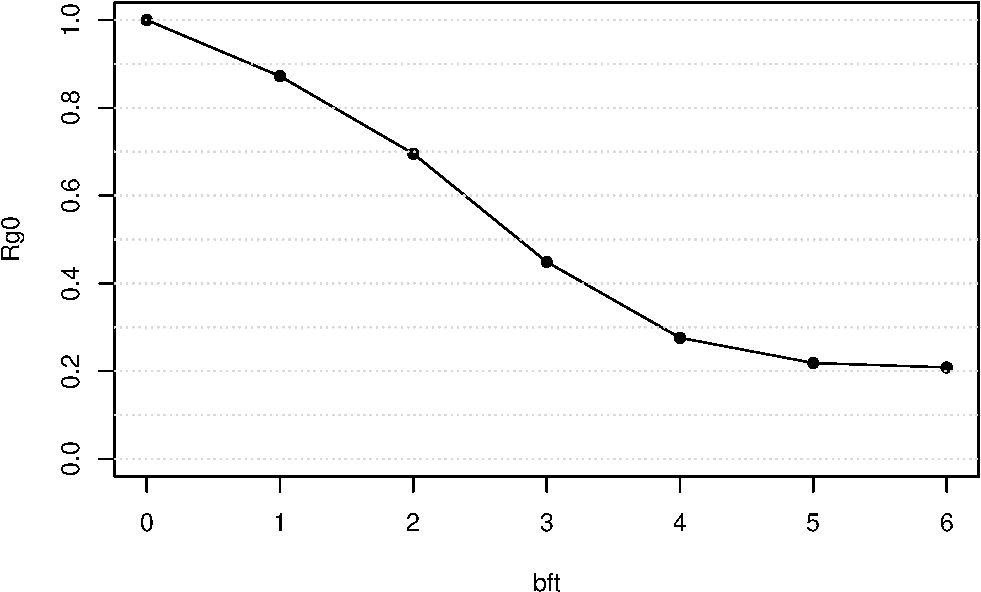
\includegraphics{figures/unnamed-chunk-142-1.pdf}

In addition to the summary above, this function returns various details, including the details of the Generalized Additive Model (GAM) (for both the estimate and the jackknifed datasets), and the raw sightings and segments used in the model.

\begin{verbatim}
[1] "Rg0"       "gam"       "jackknife" "summary"   "sightings" "segments" 
\end{verbatim}

To produce these estimates efficiently for many species, you can use the wrapper function \texttt{g0\_table()}, as follows. First you build a list of parameters for each species/species group:

\begin{Shaded}
\begin{Highlighting}[]
\NormalTok{species <-}\StringTok{ }\KeywordTok{list}\NormalTok{(}
  \KeywordTok{list}\NormalTok{(}\DataTypeTok{spp =} \KeywordTok{c}\NormalTok{(}\StringTok{'005'}\NormalTok{, }\StringTok{'016'}\NormalTok{, }\StringTok{'017'}\NormalTok{),}
       \DataTypeTok{title =} \StringTok{'Delphinus spp'}\NormalTok{,}
       \DataTypeTok{truncation =} \FloatTok{5.5}\NormalTok{),}
  \KeywordTok{list}\NormalTok{(}\DataTypeTok{spp =} \StringTok{'021'}\NormalTok{,}
       \DataTypeTok{title =} \StringTok{"Risso's dolphin"}\NormalTok{,}
       \DataTypeTok{truncation =} \FloatTok{5.5}\NormalTok{, }
       \DataTypeTok{pool_bft =} \StringTok{'12'}\NormalTok{),}
  \KeywordTok{list}\NormalTok{(}\DataTypeTok{spp =} \StringTok{'046'}\NormalTok{,}
       \DataTypeTok{title =} \StringTok{'Sperm whale'}\NormalTok{,}
       \DataTypeTok{truncation =} \FloatTok{5.5}\NormalTok{),}
  \KeywordTok{list}\NormalTok{(}\DataTypeTok{spp =} \KeywordTok{c}\NormalTok{(}\StringTok{'047'}\NormalTok{, }\StringTok{'048'}\NormalTok{, }\StringTok{'080'}\NormalTok{),}
       \DataTypeTok{title =} \StringTok{'Kogia spp'}\NormalTok{,}
       \DataTypeTok{truncation =} \FloatTok{4.0}\NormalTok{),}
  \KeywordTok{list}\NormalTok{(}\DataTypeTok{spp =} \StringTok{'061'}\NormalTok{,}
       \DataTypeTok{title =} \StringTok{"Cuvier's beaked whale"}\NormalTok{,}
       \DataTypeTok{truncation =} \FloatTok{4.0}\NormalTok{),}
  \KeywordTok{list}\NormalTok{(}\DataTypeTok{spp =} \StringTok{'074'}\NormalTok{,}
       \DataTypeTok{title =} \StringTok{'Fin whale'}\NormalTok{,}
       \DataTypeTok{truncation =} \FloatTok{5.5}\NormalTok{,}
       \DataTypeTok{regions =} \StringTok{'CCS'}\NormalTok{))}
\end{Highlighting}
\end{Shaded}

\begin{itemize}
\item
  Note that we used shorter truncation distances for cryptic species.
\item
  Note also that we had to pool Beaufort sea states 0-2 for Risso's dolphins in order to maintain a monotonic decline in the \emph{Rg(0)} \textasciitilde{} Beaufort curve.
\item
  Note also that we limited the geostrata used to model the fin whale \emph{Rg(0)} curve to the California Current System (`CCS', after Barlow 2015), so that zero-inflated segments did not confound the model.
\end{itemize}

We then pass this species list to \texttt{g0\_table()}. In this example, we are only estimating the \emph{Rg(0)} relationship, without conducting jackknife estimation:

\begin{Shaded}
\begin{Highlighting}[]
\NormalTok{rg0s <-}\StringTok{ }\KeywordTok{g0_table}\NormalTok{(cruzi,}
\NormalTok{               species,}
               \DataTypeTok{eff_types =} \StringTok{'S'}\NormalTok{,}
               \DataTypeTok{jackknife_fraction =} \OtherTok{NULL}\NormalTok{)}
\end{Highlighting}
\end{Shaded}

Now plot the result using a dedicated \texttt{LTabundR} function:

\begin{Shaded}
\begin{Highlighting}[]
\KeywordTok{g0_plot}\NormalTok{(rg0s, }\DataTypeTok{panes=}\DecValTok{1}\NormalTok{)}
\end{Highlighting}
\end{Shaded}

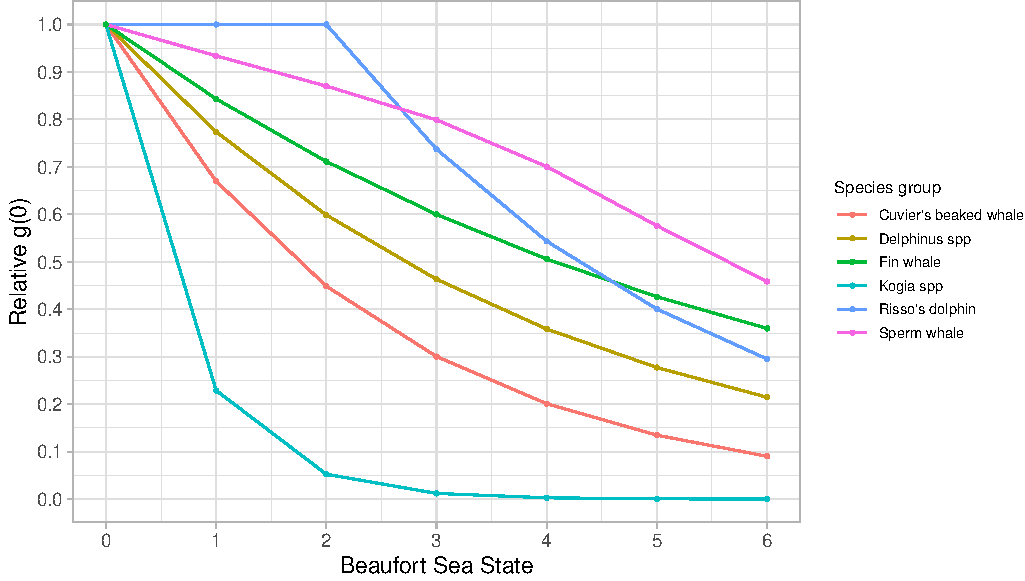
\includegraphics{figures/unnamed-chunk-148-1.pdf}

\hypertarget{weighted-average-g0}{%
\section*{\texorpdfstring{Weighted average \texttt{g(0)}}{Weighted average g(0)}}\label{weighted-average-g0}}
\addcontentsline{toc}{section}{Weighted average \texttt{g(0)}}

Since \texttt{g(0)} clearly depends upon survey conditions, and since each survey is carried out in a specific sequence of conditions, a unique, weighted \texttt{g(0)} value must be estimated for each species in each geostratum and year of interest.

This will be done automatically by the line-transect analysis functions coming up (see \texttt{LTabundR::lta()}), meaning you only need a table of \emph{Rg(0)} values in order to proceed to the next step. But you can also calculate weighted \emph{g(0)} values separately as an isolated analysis, which we show below.

Let's say we want to estimate the average \texttt{g(0)} for striped dolphins during the WHICEAS survey years of 2017 and 2020. From above, we have an estimate of the \emph{Rg(0)} and its CV for each Beaufort state:

\begin{Shaded}
\begin{Highlighting}[]
\NormalTok{rg0}\OperatorTok{$}\NormalTok{summary }\OperatorTok\StringTok{ }\KeywordTok{select}\NormalTok{(bft, Rg0, Rg0_CV)}
\NormalTok{  bft       Rg0     Rg0_CV}
\DecValTok{1}   \DecValTok{0} \FloatTok{1.0000000} \FloatTok{0.00000000}
\DecValTok{2}   \DecValTok{1} \FloatTok{0.8721458} \FloatTok{0.08129651}
\DecValTok{3}   \DecValTok{2} \FloatTok{0.6955418} \FloatTok{0.13915558}
\DecValTok{4}   \DecValTok{3} \FloatTok{0.4490084} \FloatTok{0.14602914}
\DecValTok{5}   \DecValTok{4} \FloatTok{0.2760549} \FloatTok{0.13552456}
\DecValTok{6}   \DecValTok{5} \FloatTok{0.2185606} \FloatTok{0.14985606}
\DecValTok{7}   \DecValTok{6} \FloatTok{0.2085412} \FloatTok{0.20814588}
\end{Highlighting}
\end{Shaded}

We also have a processed \texttt{cruz} object with 2017 data:

\begin{Shaded}
\begin{Highlighting}[]
\KeywordTok{load}\NormalTok{(}\StringTok{'whiceas_cruz_1720.RData'}\NormalTok{)}
\NormalTok{cruz_}\DecValTok{17}\NormalTok{ <-}\StringTok{ }\KeywordTok{filter_cruz}\NormalTok{(cruz_}\DecValTok{1720}\NormalTok{, }\DataTypeTok{years =} \DecValTok{2017}\NormalTok{, }\DataTypeTok{verbose=}\OtherTok{FALSE}\NormalTok{)}
\end{Highlighting}
\end{Shaded}

To view the distribution of effort in this WHICEAS 2017 across sea states, we can use the function \texttt{summarize\_bft()}:

\begin{Shaded}
\begin{Highlighting}[]
\KeywordTok{summarize_bft}\NormalTok{(cruz_}\DecValTok{17}\NormalTok{)}\OperatorTok{$}\NormalTok{overall}
\CommentTok{# A tibble: 6 x 3}
\NormalTok{   bftr    km   prop}
  \OperatorTok{<}\NormalTok{dbl}\OperatorTok{>}\StringTok{ }\ErrorTok{<}\NormalTok{dbl}\OperatorTok{>}\StringTok{  }\ErrorTok{<}\NormalTok{dbl}\OperatorTok{>}
\DecValTok{1}     \DecValTok{1}  \FloatTok{130.} \FloatTok{0.0200}
\DecValTok{2}     \DecValTok{2}  \FloatTok{583.} \FloatTok{0.0897}
\DecValTok{3}     \DecValTok{3}  \FloatTok{901.} \FloatTok{0.139} 
\DecValTok{4}     \DecValTok{4} \FloatTok{2140.} \FloatTok{0.329} 
\DecValTok{5}     \DecValTok{5} \FloatTok{1873.} \FloatTok{0.288} 
\DecValTok{6}     \DecValTok{6}  \FloatTok{875.} \FloatTok{0.135} 
\end{Highlighting}
\end{Shaded}

We then use the function \texttt{g0\_weighted\_var()} to compute the weighted \emph{Rg(0)} for our survey as well as its CV. This function carries out an automated optimization routine to simulate a new distribution for the weighted \emph{g(0)}, which is then used to estimate the weighted CV.

\begin{Shaded}
\begin{Highlighting}[]
\NormalTok{weighted_g0_}\DecValTok{2017}\NormalTok{ <-}\StringTok{ }
\StringTok{  }\KeywordTok{g0_weighted}\NormalTok{(}\DataTypeTok{Rg0 =}\NormalTok{ rg0}\OperatorTok{$}\NormalTok{summary}\OperatorTok{$}\NormalTok{Rg0,}
              \DataTypeTok{Rg0_cv =}\NormalTok{ rg0}\OperatorTok{$}\NormalTok{summary}\OperatorTok{$}\NormalTok{Rg0_CV, }
              \DataTypeTok{cruz =}\NormalTok{ cruz_}\DecValTok{17}\NormalTok{)}
\end{Highlighting}
\end{Shaded}

The result:

\begin{Shaded}
\begin{Highlighting}[]
\NormalTok{weighted_g0_}\DecValTok{2017}\OperatorTok{$}\NormalTok{g0[}\DecValTok{1}\OperatorTok{:}\DecValTok{2}\NormalTok{]}
\NormalTok{  wt.mean wt.cv}
\DecValTok{1}   \FloatTok{0.326} \FloatTok{0.143}
\end{Highlighting}
\end{Shaded}

Now let's do the same for WHICEAS 2020 and compare the weighted \emph{g(0)} estimate:

\begin{Shaded}
\begin{Highlighting}[]
\CommentTok{# Filter to 2020}
\NormalTok{cruz_}\DecValTok{20}\NormalTok{ <-}\StringTok{ }\KeywordTok{filter_cruz}\NormalTok{(cruz_}\DecValTok{1720}\NormalTok{, }\DataTypeTok{years =} \DecValTok{2020}\NormalTok{, }\DataTypeTok{verbose=}\OtherTok{FALSE}\NormalTok{)}

\CommentTok{# Summarize Bft effort}
\KeywordTok{summarize_bft}\NormalTok{(cruz_}\DecValTok{20}\NormalTok{)}\OperatorTok{$}\NormalTok{overall}
\CommentTok{# A tibble: 6 x 3}
\NormalTok{   bftr     km   prop}
  \OperatorTok{<}\NormalTok{dbl}\OperatorTok{>}\StringTok{  }\ErrorTok{<}\NormalTok{dbl}\OperatorTok{>}\StringTok{  }\ErrorTok{<}\NormalTok{dbl}\OperatorTok{>}
\DecValTok{1}     \DecValTok{1}   \FloatTok{88.2} \FloatTok{0.0165}
\DecValTok{2}     \DecValTok{2}  \FloatTok{262.}  \FloatTok{0.0490}
\DecValTok{3}     \DecValTok{3}  \FloatTok{434.}  \FloatTok{0.0813}
\DecValTok{4}     \DecValTok{4} \FloatTok{1482.}  \FloatTok{0.278} 
\DecValTok{5}     \DecValTok{5} \FloatTok{2004.}  \FloatTok{0.376} 
\DecValTok{6}     \DecValTok{6} \FloatTok{1067.}  \FloatTok{0.200} 
\end{Highlighting}
\end{Shaded}

Note that conditions were a bit worse in 2020 compared to 2017. We therefore expect the weighted \emph{g(0)} estimate to be lower:

\begin{Shaded}
\begin{Highlighting}[]
\NormalTok{weighted_g0_}\DecValTok{2020}\NormalTok{ <-}\StringTok{ }
\StringTok{  }\KeywordTok{g0_weighted}\NormalTok{(}\DataTypeTok{Rg0 =}\NormalTok{ rg0}\OperatorTok{$}\NormalTok{summary}\OperatorTok{$}\NormalTok{Rg0,}
              \DataTypeTok{Rg0_cv =}\NormalTok{ rg0}\OperatorTok{$}\NormalTok{summary}\OperatorTok{$}\NormalTok{Rg0_CV, }
              \DataTypeTok{cruz =}\NormalTok{ cruz_}\DecValTok{20}\NormalTok{)}
\end{Highlighting}
\end{Shaded}

The result:

\begin{Shaded}
\begin{Highlighting}[]
\NormalTok{weighted_g0_}\DecValTok{2020}\OperatorTok{$}\NormalTok{g0[}\DecValTok{1}\OperatorTok{:}\DecValTok{2}\NormalTok{]}
\NormalTok{  wt.mean wt.cv}
\DecValTok{1}   \FloatTok{0.286} \FloatTok{0.149}
\end{Highlighting}
\end{Shaded}

Confirmed: weighted \emph{g(0)} for 2020 is slightly lower than in 2017, due to generally worse survey conditions. These year-specific estimates should prevent those different conditions from impacting their respective abundance estimates.

\hypertarget{lta}{%
\chapter{Line-transect analysis}\label{lta}}

We use line-transect analysis to produce estimates of animal density and/or abundance based upon surveys. The main \texttt{LTabundR} function for conducting line-transect analysis is \texttt{lta()}, which calls for four primary arguments in addition to your \texttt{cruz} object:

\begin{Shaded}
\begin{Highlighting}[]
\KeywordTok{lta}\NormalTok{(cruz,}
\NormalTok{    Rg0,}
\NormalTok{    fit_filters,}
\NormalTok{    df_settings,}
\NormalTok{    estimates)}
\end{Highlighting}
\end{Shaded}

Below we explain each of these inputs, discuss other optional inputs, and explore the results produced by \texttt{lta()}.

\hypertarget{key-inputs}{%
\section*{Key inputs}\label{key-inputs}}
\addcontentsline{toc}{section}{Key inputs}

\hypertarget{cruz}{%
\subsection*{\texorpdfstring{\texttt{cruz}}{cruz}}\label{cruz}}
\addcontentsline{toc}{subsection}{\texttt{cruz}}

This is the \texttt{cruz} object you have generated with \texttt{process\_surveys()}. Before running \texttt{lta()}, ensure that this \texttt{cruz} object is filtered only to the years, regions, and sighting conditions you would like to use for detection function fitting. Filter your cruz object with full flexibility using \texttt{LTabundR::filter\_cruz()}. Note that filtering for detection function fitting is typically less stringent than filtering for downstream steps for abundance estimation, since as many sightings are included as possible to combat low sample sizes, as long as sightings were observed using standard methods in an unbiased search pattern, and as long as you do not expect detectability to vary across years and regions.

Here we will work with a version of the 1986-2020 Central North Pacific survey data we processed a few pages back. This version is included as a built-in dataset within \texttt{LTabundR}:

\begin{Shaded}
\begin{Highlighting}[]
\KeywordTok{data}\NormalTok{(}\StringTok{"cnp_150km_1986_2020"}\NormalTok{)}
\NormalTok{cruz <-}\StringTok{ }\NormalTok{cnp_150km_}\DecValTok{1986}\NormalTok{_}\DecValTok{2020}
\end{Highlighting}
\end{Shaded}

As it is provided, this dataset does not need any filtering.

We will use these data to estimate the abundance of striped dolphins (\emph{Stenella coeruleoalba}), Fraser's dolphins (\emph{Lagenodelphis hosei}), and Melon-headed whales (\emph{Preponocephala electra}) within the WHICEAS study area in 2017 and 2020. We will group these three species into a `species pool' in order to gain a sufficient sample size for fitting a detection function. We will then use ``Species'' as a covariate within the detection function model, along with other variables including Beaufort Sea State, ship name, and log-transformed school size.

\hypertarget{rg0}{%
\subsection*{\texorpdfstring{\texttt{Rg0}}{Rg0}}\label{rg0}}
\addcontentsline{toc}{subsection}{\texttt{Rg0}}

The result of \texttt{LTabundR::g0\_model()}, which is a \texttt{data.frame} with Relative trackline detection probabilities, \emph{Rg(0)}, for each species in each Beaufort sea state. See \texttt{LTabundR} dataset \texttt{data("g0\_results")}, used below, as an example.

This is an \emph{optional} input. If not provided, \emph{g(0)} will be assumed to 1.0, and its CV will be assumed to be 0. Alternatively, you can manually specify values for \emph{g(0)} and its CV in the \texttt{estimates} argument below.

Here we will use a \texttt{data.frame} of \emph{Rg(0)} estimates based on the same survey years, 1986 - 2020, which has been provided as a built-in dataset:

\begin{Shaded}
\begin{Highlighting}[]
\KeywordTok{data}\NormalTok{(}\StringTok{"g0_results"}\NormalTok{)}
\NormalTok{Rg0 <-}\StringTok{ }\NormalTok{g0_results}
\end{Highlighting}
\end{Shaded}

\hypertarget{fit_filters}{%
\subsection*{\texorpdfstring{\texttt{fit\_filters}}{fit\_filters}}\label{fit_filters}}
\addcontentsline{toc}{subsection}{\texttt{fit\_filters}}

The \texttt{fit\_filters} input specifies how to filter the data before fitting the detection function. It accepts a named list, which in our example will look like this:

\begin{Shaded}
\begin{Highlighting}[]
\NormalTok{fit_filters =}\StringTok{ }\KeywordTok{list}\NormalTok{(}\DataTypeTok{spp =} \KeywordTok{c}\NormalTok{(}\StringTok{'013'}\NormalTok{, }\StringTok{'026'}\NormalTok{, }\StringTok{'031'}\NormalTok{), }
                   \DataTypeTok{pool =} \StringTok{'Multi-species pool 1'}\NormalTok{,}
                   \DataTypeTok{cohort =} \StringTok{'all'}\NormalTok{,}
                   \DataTypeTok{truncation_distance =} \DecValTok{5}\NormalTok{,}
                   \DataTypeTok{other_species =} \StringTok{'remove'}\NormalTok{)}
\end{Highlighting}
\end{Shaded}

\begin{itemize}
\item
  \textbf{\texttt{spp}}: A character vector of species codes. Using multiple species codes may be useful when you have low sample sizes for a cohort of similar species.
\item
  \textbf{\texttt{cohort}}: The cohort containing these species, provided as a name or a number indicating which slot in \texttt{cruz\$cohorts} should be referenced.
\item
  \textbf{\texttt{truncation\_distance}}: The truncation distance to apply during model fitting.
\end{itemize}

\emph{The remaining inputs are optional (i.e., they all have defaults):}

\begin{itemize}
\item
  \textbf{\texttt{pool}}: A character string, providing a title for this species pool. If not specified, the species codes used will be concatenated to produce a title automatically.
\item
  \textbf{\texttt{other\_species}}: A character vector with four recognized values:

  \begin{itemize}
  \tightlist
  \item
    If \texttt{"apply"} (the default if not specified), the species code will be changed to \texttt{"Other"} for sightings in which the species was in a mixed-species school but was not the species with the largest percentage of the total school size. In those cases, the species was not as relevant to the detection of the school as the other species were, which may bias the detection function. This creates a factor level for the detection function to use (when \texttt{"species"} is a covariate) to distinguish between cue-relevant species that are within the specified pool and those that are not.
  \item
    The second option for \texttt{other\_species} is \texttt{"ignore"}, which does \textbf{not} reassign species codes to \texttt{"Other"}, and ignores whether the species of interest held the plurality for a mixed species detection.
  \item
    The third option is \texttt{"remove"}: any species re-assigned to \texttt{"Other"} will be removed before the detection function is fit; this can be useful if only a small number of species are re-assigned to \texttt{"Other"}, which would then obviate \texttt{species} as a viable covariate (since the sample size of all \texttt{species} levels would be unlikely to exceed \texttt{df\_settings\$covariates\_n\_per\_level} -- see below). 
  \item
    The fourth and final option is \texttt{coerce}, which forces \emph{all} species codes to \texttt{"Other"} for the purposes of detection function fitting and abundance estimation. This is effectively the same as removing `species' from the list of covariates, but this option can be a convenience if you want to quickly toggle the use of \texttt{species} as a covariate for a specific species pool, and/or produce abundance estimates for unidentified taxa (e.g., an `Unidentified dolphins' species pool that includes multiple species codes).
  \end{itemize}
\end{itemize}

~

\hypertarget{df_settings}{%
\subsection*{\texorpdfstring{\texttt{df\_settings}}{df\_settings}}\label{df_settings}}
\addcontentsline{toc}{subsection}{\texttt{df\_settings}}

The \texttt{df\_settings} input specifies how to fit a detection function to the filtered data. It accepts a named list, which in our example will look like this:

\begin{Shaded}
\begin{Highlighting}[]
\NormalTok{df_settings =}\StringTok{ }\KeywordTok{list}\NormalTok{(}\DataTypeTok{covariates =} \KeywordTok{c}\NormalTok{(}\StringTok{'bft'}\NormalTok{,}\StringTok{'lnsstot'}\NormalTok{,}\StringTok{'cruise'}\NormalTok{,}\StringTok{'year'}\NormalTok{,}\StringTok{'ship'}\NormalTok{,}\StringTok{'species'}\NormalTok{),}
                   \DataTypeTok{covariates_factor =} \KeywordTok{c}\NormalTok{(}\OtherTok{FALSE}\NormalTok{, }\OtherTok{FALSE}\NormalTok{, }\OtherTok{TRUE}\NormalTok{, }\OtherTok{TRUE}\NormalTok{, }\OtherTok{TRUE}\NormalTok{, }\OtherTok{TRUE}\NormalTok{),}
                   \DataTypeTok{covariates_levels =} \DecValTok{2}\NormalTok{,}
                   \DataTypeTok{covariates_n_per_level =} \DecValTok{10}\NormalTok{,}
                   \DataTypeTok{detection_function_base =} \StringTok{'hn'}\NormalTok{,}
                   \DataTypeTok{base_model =} \StringTok{'~1'}\NormalTok{,}
                   \DataTypeTok{delta_aic =} \DecValTok{2}\NormalTok{)}
\end{Highlighting}
\end{Shaded}

\emph{(Note that all of these inputs have defaults, and are therefore optional.)}

\begin{itemize}
\item
  \textbf{\texttt{covariates}} Covariates you wish to include as candidates in detection function models, provided as a character vector. The covariates must match columns existing within \texttt{cruz\$cohorts\$\textless{}cohort\_name\textgreater{}\$sightings}. Note that the function will ignore case, coercing all covariates to lowercase. Default: no covariates.
\item
  \textbf{\texttt{covariates\_factor}} A Boolean vector, which must be the same length as \texttt{covariates}, indicating whether each covariate should be treated as a factor instead of a numeric. Default: \texttt{NULL}.
\item
  \textbf{\texttt{covariates\_levels}} The minimum number of levels a factor covariate must have in order to be included as an eligible covariate. Default: \texttt{2}.
\item
  \textbf{\texttt{covariates\_n\_per\_level}} The minimum number of observations within each level of a factor covariate. If this condition is not met, the covariate is excluded from the candidates. Default: \texttt{10}.
\item
  \textbf{\texttt{detection\_function\_base}} The base key for the detection function, provided as a character vector. Accepted values are \texttt{"hn"} (half-normal key, the default, which exhibits greater stability when fitting to cetacean survey data; Gerrogette and Forcada 2005), \texttt{"hr"} (hazard-rate), or \texttt{c("hn",\ "hr)}, which will loop through both keys and attempt model fitting.
\item
  \textbf{\texttt{base\_model}} The initial model formula, upon which to build using candidate covariates. If not provided by the user, the default is \texttt{"\textasciitilde{}\ 1"}.
\item
  \textbf{\texttt{delta\_aic}} The AIC difference between the model yielding the lowest AIC and other candidate models, used to define the best-fitting models. Typically, AIC differences of less than 2 (the default) indicate effectively equal model performance. If this value is not zero, then model averaging will be done: if multiple models are within \texttt{delta\_aic} of the model with the lowest AIC, all ``best'' models will be used in subsequent steps and their results will be averaged. See \texttt{Details} below.
\end{itemize}

\hypertarget{estimates}{%
\subsection*{\texorpdfstring{\texttt{estimates}}{estimates}}\label{estimates}}
\addcontentsline{toc}{subsection}{\texttt{estimates}}

The \texttt{estimates} input specifies which estimates of density and abundance to produce based on the fitted detection function. This input accepts a list of sub-lists, which in our example will look something like this:

\begin{Shaded}
\begin{Highlighting}[]
\NormalTok{estimates <-}\StringTok{ }\KeywordTok{list}\NormalTok{(}\KeywordTok{list}\NormalTok{(}\DataTypeTok{spp =} \StringTok{'013'}\NormalTok{,}
                       \DataTypeTok{title =} \StringTok{'Striped dolphin'}\NormalTok{,}
                       \DataTypeTok{years =} \DecValTok{2017}\NormalTok{,}
                       \DataTypeTok{regions =} \StringTok{'WHICEAS'}\NormalTok{))}
\end{Highlighting}
\end{Shaded}

This example shows only a single sub-list, specifying how to generate a density/abundance estimate for striped dolphins (species code 013) within the ``WHICEAS'' geostratum for 2017.

\begin{itemize}
\item
  \textbf{\texttt{spp}}: A character vector of species codes.
\item
  \textbf{\texttt{title}}: A title for this abundance estimate, given as a character vector, ' e.g., \texttt{"Striped\ dolphin\ -\ pelagic"}. If left blank, the species code(s) will be concatenated to use as a title.
\item
  \textbf{\texttt{years}}: A numeric vector of years, used to filter data to include only effort/sightings from these years.
\item
  \textbf{\texttt{regions}}: A character vector of geostratum names, used to filter the data. Any segment or sighting occurring within \emph{any} (but \emph{not} necessarily all) of the provided \texttt{regions} will be returned. This holds true for nested regions: for example, in analyses from the Central North Pacific, in which the Hawaii EEZ geostratum (\texttt{"HI-EEZ"}) is nested within the larger geostratum representing the entire CNP study area (\texttt{"OtherCNP"}), an input of \texttt{regions\ =\ "OtherCNP"} will return segments/sightings \emph{both} inside the Hawaii EEZ \emph{and} outside of it.
\end{itemize}

You also have the option of manually specifying other filters \& arguments. Each of these sub-lists accepts the following named slots:

\begin{itemize}
\item
  \textbf{\texttt{cruises}}: An optional numeric vector of cruise numbers, used to filter data to include effort/sighting from only certain cruises. Ignored if \texttt{NULL.}
\item
  \textbf{\texttt{regions\_remove}}: A character vector of geostratum names, similar to above. Any segment or sighting occurring within any of these \texttt{not\_regions} will \textbf{not} be returned. Using the example above, if \texttt{regions\ =\ "OtherCNP"} and \texttt{not\_regions\ =\ "HI-EEZ"}, only segments occuring within \texttt{OtherCNP} \emph{and} outside of \texttt{HI-EEZ} will be returned. This can be particularly useful for abundance estimates for pelagic stock that exclude nested insular stocks.
\item
  \textbf{\texttt{g0}}: If left as the default \texttt{NULL}, the \texttt{lta()} function will automatically estimate the weighted trackline detection probability \emph{(g0)} according to the distribution of Beaufort sea states contained within the survey years/regions for which density/abundance is being estimated (this is done using the \texttt{LTabundR} function \texttt{g0\_weighted()}). This will only be done if the \texttt{Rg0} input above is not \texttt{NULL}; if it is and you do not provide \emph{g(0)} values here, \texttt{g0} will be coerced to equal 1. To coerce \texttt{g(0)} to a certain value of your own choosing, you can provide a numeric vector of length 1 or 2. If length 1, this value represents \emph{g(0)} for all schools regardless of size. If length 2, these values represent \emph{g(0)} for small and large school sizes, as defined by \texttt{g0\_threshold} below.
\item
  \textbf{\texttt{g0\_cv}}: Similar to g0 above: if left \texttt{NULL}, the CV of the \texttt{g(0)} estimate will be automatically estimated based on weighted survey conditions. Alternatively, you can manually specify a CV here, using a numeric vector of length 1 or 2. If you do not specify a value and \texttt{Rg0} input is NULL, \texttt{g0\_cv} will be coerced to equal 0.
\item
  \textbf{\texttt{g0\_threshold}}: The school size threshold between small and large groups.
\item
  \textbf{\texttt{alt\_g0\_spp}}: An alternate species code to use to draw Relative \emph{g(0)} values from the \texttt{Rg0} input. This is useful in the event that \emph{Rg(0)} was not estimated for the species whose density/abundance you are estimating, but there is a similarly detectable species whose \emph{Rg(0)} parameters have been estimated.
\item
  \textbf{\texttt{combine\_g0}}: A Boolean, with default \texttt{FALSE}. If \texttt{TRUE}, weighted \emph{g0} estimates will be produced separately for each species code provided (specifically, for each unique row in the \texttt{Rg0} table that is found after filtering by the species codes you provide in this estimate), \emph{THEN} average those estimates together. This can be useful when you do not have a \emph{Rg(0)} estimates for a certain species, but you can approximate \emph{g0} by averaging together estimates from multiple species (e.g., averaging together weighted \emph{g(0)} from across rorqual species in order to get a weighted \emph{g(0)} estimate for `Unidentified rorquals').
\item
  \textbf{\texttt{region\_title}}: An optional character vector indicating the title you would like to give to the region pertaining to this estimate. This can be useful if you have a complicated assemblage of regions you are combining and/or removing. If not supplied, the function will automatically generate a \texttt{region\_title} based on \texttt{regions} and \texttt{regions\_remove}.
\item
  \textbf{\texttt{forced\_effort}}: If this is a single numeric value instead of \texttt{NULL} (\texttt{NULL} is the default), this value will be used as the survey effort, in km, in a brute-force method; this same value will be used for every year and region. This is only helpful if you are looking for a relatively easy way to compare results from your own analysis to another (e.g., comparing \texttt{LTabundR} results to reports from NOAA reports prior to 2021, in which effort was calculated slightly differently).
\item
  \textbf{\texttt{area}}: If this is a single numeric value instead of \texttt{NULL} (\texttt{NULL} is the default), this value will be used as the area of the region in which abundance is being estimated, in square km, in a brute-force approach. If left \texttt{NULL}, the function will calculate the final area of the survey area resulting from the regions and regions\_remove filters above.
\item
  \textbf{\texttt{remove\_land}}: A Boolean, with default \texttt{TRUE}, indicating whether or not land area should be removed from the survey area before calculating its area for abundance estimation. This term is only referenced if area is not specified manually.
\end{itemize}

Here is the full \texttt{estimates} list for all the species-year-geostratum combinations for which we want to estimate density/abundance:

\begin{Shaded}
\begin{Highlighting}[]
\NormalTok{estimates <-}\StringTok{ }\KeywordTok{list}\NormalTok{(}
    \KeywordTok{list}\NormalTok{(}\DataTypeTok{spp =} \StringTok{'013'}\NormalTok{,}
         \DataTypeTok{title =} \StringTok{'Striped dolphin'}\NormalTok{,}
         \DataTypeTok{years =} \DecValTok{2017}\NormalTok{,}
         \DataTypeTok{regions =} \StringTok{'WHICEAS'}\NormalTok{),}
    \KeywordTok{list}\NormalTok{(}\DataTypeTok{spp =} \StringTok{'013'}\NormalTok{,}
         \DataTypeTok{title =} \StringTok{'Striped dolphin'}\NormalTok{,}
         \DataTypeTok{years =} \DecValTok{2020}\NormalTok{,}
         \DataTypeTok{regions =} \StringTok{'WHICEAS'}\NormalTok{),}
    \KeywordTok{list}\NormalTok{(}\DataTypeTok{spp =} \StringTok{'026'}\NormalTok{,}
         \DataTypeTok{title =} \StringTok{'Frasers dolphin'}\NormalTok{,}
         \DataTypeTok{years =} \DecValTok{2017}\NormalTok{,}
         \DataTypeTok{regions =} \StringTok{'WHICEAS'}\NormalTok{),}
    \KeywordTok{list}\NormalTok{(}\DataTypeTok{spp =} \StringTok{'026'}\NormalTok{,}
         \DataTypeTok{title =} \StringTok{'Frasers dolphin'}\NormalTok{,}
         \DataTypeTok{years =} \DecValTok{2020}\NormalTok{,}
         \DataTypeTok{regions =} \StringTok{'WHICEAS'}\NormalTok{),}
    \KeywordTok{list}\NormalTok{(}\DataTypeTok{spp =} \StringTok{'031'}\NormalTok{,}
         \DataTypeTok{title =} \StringTok{'Melon-headed whale'}\NormalTok{,}
         \DataTypeTok{years =} \DecValTok{2017}\NormalTok{,}
         \DataTypeTok{regions =} \StringTok{'WHICEAS'}\NormalTok{),}
    \KeywordTok{list}\NormalTok{(}\DataTypeTok{spp =} \StringTok{'031'}\NormalTok{,}
         \DataTypeTok{title =} \StringTok{'Melon-headed whale'}\NormalTok{,}
         \DataTypeTok{years =} \DecValTok{2020}\NormalTok{,}
         \DataTypeTok{regions =} \StringTok{'WHICEAS'}\NormalTok{))}
\end{Highlighting}
\end{Shaded}

Each of these sub-lists specifies the details for a single estimate of density/abundance, making it possible to produce multiple estimates from the same detection function model. Generally, there needs to be a sub-list for each species-region-year combination of interest.

Quickly review results:

\begin{Shaded}
\begin{Highlighting}[]
\NormalTok{results}\OperatorTok{$}\NormalTok{estimate}
\NormalTok{               title species    Region     Area year segments       km}
\DecValTok{1}\NormalTok{    Striped dolphin     }\DecValTok{013}\NormalTok{ (WHICEAS) }\FloatTok{402948.7} \DecValTok{2017}       \DecValTok{38} \FloatTok{3040.009}
\DecValTok{2}\NormalTok{    Striped dolphin     }\DecValTok{013}\NormalTok{ (WHICEAS) }\FloatTok{402948.7} \DecValTok{2020}       \DecValTok{40} \FloatTok{4585.386}
\DecValTok{3}\NormalTok{    Frasers dolphin     }\DecValTok{026}\NormalTok{ (WHICEAS) }\FloatTok{402948.7} \DecValTok{2020}       \DecValTok{40} \FloatTok{4585.386}
\DecValTok{4}\NormalTok{ Melon}\OperatorTok{-}\NormalTok{headed whale     }\DecValTok{031}\NormalTok{ (WHICEAS) }\FloatTok{402948.7} \DecValTok{2017}       \DecValTok{38} \FloatTok{3040.009}
\DecValTok{5}\NormalTok{ Melon}\OperatorTok{-}\NormalTok{headed whale     }\DecValTok{031}\NormalTok{ (WHICEAS) }\FloatTok{402948.7} \DecValTok{2020}       \DecValTok{40} \FloatTok{4585.386}
\NormalTok{  Area_covered ESW_mean n g0_est  ER_clusters   D_clusters N_clusters size_mean}
\DecValTok{1}      \FloatTok{9610.88} \FloatTok{3.161465} \DecValTok{3}  \FloatTok{0.315} \FloatTok{0.0009868393} \FloatTok{0.0005020214}  \FloatTok{202.28888}  \FloatTok{31.95079}
\DecValTok{2}     \FloatTok{16236.27} \FloatTok{3.540874} \DecValTok{3}  \FloatTok{0.280} \FloatTok{0.0006542525} \FloatTok{0.0003299532}  \FloatTok{132.95423}  \FloatTok{53.95865}
\DecValTok{3}     \FloatTok{17084.73} \FloatTok{3.725909} \DecValTok{2}  \FloatTok{0.446} \FloatTok{0.0004361683} \FloatTok{0.0001312386}   \FloatTok{52.88243} \FloatTok{132.51143}
\DecValTok{4}     \FloatTok{10669.12} \FloatTok{3.509569} \DecValTok{2}  \FloatTok{0.511} \FloatTok{0.0006578929} \FloatTok{0.0001835580}   \FloatTok{73.96447} \FloatTok{185.98103}
\DecValTok{5}     \FloatTok{16949.65} \FloatTok{3.696451} \DecValTok{3}  \FloatTok{0.483} \FloatTok{0.0006542525} \FloatTok{0.0001832491}   \FloatTok{73.84001} \FloatTok{226.13289}
\NormalTok{      size_sd         ER          D         N}
\DecValTok{1}   \FloatTok{0.5780968} \FloatTok{0.03153029} \FloatTok{0.01606793}  \FloatTok{6474.550}
\DecValTok{2}   \FloatTok{2.7402089} \FloatTok{0.03530258} \FloatTok{0.01780121}  \FloatTok{7172.977}
\DecValTok{3} \FloatTok{182.1747087} \FloatTok{0.05779729} \FloatTok{0.01733567}  \FloatTok{6985.385}
\DecValTok{4}  \FloatTok{96.4369707} \FloatTok{0.12235559} \FloatTok{0.03379710} \FloatTok{13618.500}
\DecValTok{5} \FloatTok{175.5620746} \FloatTok{0.14794801} \FloatTok{0.04158955} \FloatTok{16758.457}
\end{Highlighting}
\end{Shaded}

More details on the \texttt{lta()} output are provided below.

\hypertarget{variance-estimation}{%
\section*{Variance estimation}\label{variance-estimation}}
\addcontentsline{toc}{section}{Variance estimation}

By default, the \texttt{lta()} function produces a single estimate of the detection function and a single estimate of density/abundance estimate for each sub-list within \texttt{estimates()}. However, you can obtain the coefficient of variation (CV) of those estimates by activating the function's bootstrap variance estimation feature. To do this, add \texttt{bootstraps} as an input specifying a large number of iterations (1,000 iterations is standard, but we suggest first testing your code with 5 - 10 bootstraps before committing; the function typically requires \textasciitilde1 hour per 100 bootstraps.).

For the purposes of example only, we will just use 10 bootstrap iterations here:

\begin{Shaded}
\begin{Highlighting}[]
\NormalTok{results <-}\StringTok{ }\KeywordTok{lta}\NormalTok{(cruz, Rg0,}
\NormalTok{               fit_filters, df_settings, estimates,}
               \DataTypeTok{bootstraps =} \DecValTok{10}\NormalTok{)}
\end{Highlighting}
\end{Shaded}

This command will first produce official estimates of the detection function and density/abundance, then it will repeat the analysis for the number of iterations you have specified. In each iteration, survey segments are re-sampled according to standard bootstrap variance estimation methods (see more details below, in ``Behind the Scenes'').

\hypertarget{other-inputs}{%
\section*{Other inputs}\label{other-inputs}}
\addcontentsline{toc}{section}{Other inputs}

There are a few other optional input arguments that lend further control over the \texttt{lta()} procedure.

\begin{Shaded}
\begin{Highlighting}[]
\KeywordTok{lta}\NormalTok{(cruz,}
\NormalTok{    Rg0,}
\NormalTok{    fit_filters,}
\NormalTok{    df_settings,}
\NormalTok{    estimates,}
    \DataTypeTok{use_g0 =} \OtherTok{TRUE}\NormalTok{,}
    \DataTypeTok{ss_correction =} \DecValTok{1}\NormalTok{,}
    \DataTypeTok{bootstraps =} \DecValTok{10}
    \DataTypeTok{toplot =} \OtherTok{TRUE}\NormalTok{,}
    \DataTypeTok{verbose =} \OtherTok{TRUE}\NormalTok{,)}
\end{Highlighting}
\end{Shaded}

\begin{itemize}
\item
  \textbf{\texttt{use\_g0}}: A Boolean, with default \texttt{TRUE}, indicating whether or not to use custom \texttt{g(0)} value(s). If \texttt{FALSE}, the assumed \texttt{g(0)} value will be 1. This is an easy way to toggle on-and-off automated \emph{g(0)} estimation and/or ignore manually supplied \emph{g(0)} values.
\item
  \textbf{\texttt{ss\_correction}}: Should a correction be applied to school sizes? School sizes will be scaled by this number. The default, \texttt{1}, means no changes will occur.
\item
  \textbf{\texttt{toplot}}: A Boolean, with default \texttt{TRUE}, indicating whether detection function plots (\texttt{Distance::plot.ds()}) should be displayed as the candidate models are tested.
\item
  \textbf{\texttt{verbose}}: A Boolean, with default \texttt{TRUE}, indicating whether or not updates should be printed to the Console.
\end{itemize}

\hypertarget{output}{%
\section*{Output}\label{output}}
\addcontentsline{toc}{section}{Output}

\hypertarget{during-processing}{%
\subsection*{During processing}\label{during-processing}}
\addcontentsline{toc}{subsection}{During processing}

While \texttt{lta()} is running, it will print things to the Console (if \texttt{verbose} is \texttt{TRUE}), plot diagnostic plots of how the study area is being calculated (if \texttt{toplot} is \texttt{TRUE}), and plot detection function model candidates (if \texttt{toplot} is \texttt{TRUE}). To demonstrate this, we will run the estimate for striped dolphins in 2017 only, without variance bootstrapping. To expedite processing, we will manually supply \emph{g(0)} values from Bradford et al.~(2021) (this saves about 3 minutes per estimate):

\begin{Shaded}
\begin{Highlighting}[]
\NormalTok{new_estimates <-}\StringTok{ }\KeywordTok{list}\NormalTok{(}
    \KeywordTok{list}\NormalTok{(}\DataTypeTok{spp =} \StringTok{'013'}\NormalTok{,}
         \DataTypeTok{title =} \StringTok{'Striped dolphin'}\NormalTok{,}
         \DataTypeTok{years =} \DecValTok{2017}\NormalTok{,}
         \DataTypeTok{regions =} \StringTok{'WHICEAS'}\NormalTok{,}
         \DataTypeTok{g0 =} \FloatTok{0.35}\NormalTok{, }\DataTypeTok{g0_cv =} \FloatTok{0.19}\NormalTok{))}

\CommentTok{# Run it:}
\NormalTok{demo <-}\StringTok{ }\KeywordTok{lta}\NormalTok{(cruz, Rg0, fit_filters, df_settings, new_estimates)}
\end{Highlighting}
\end{Shaded}

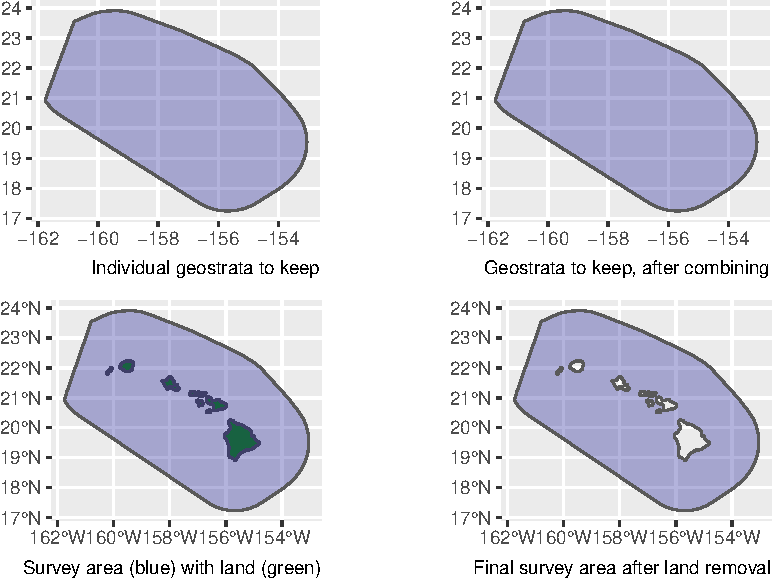
\includegraphics{figures/unnamed-chunk-177-1.pdf} 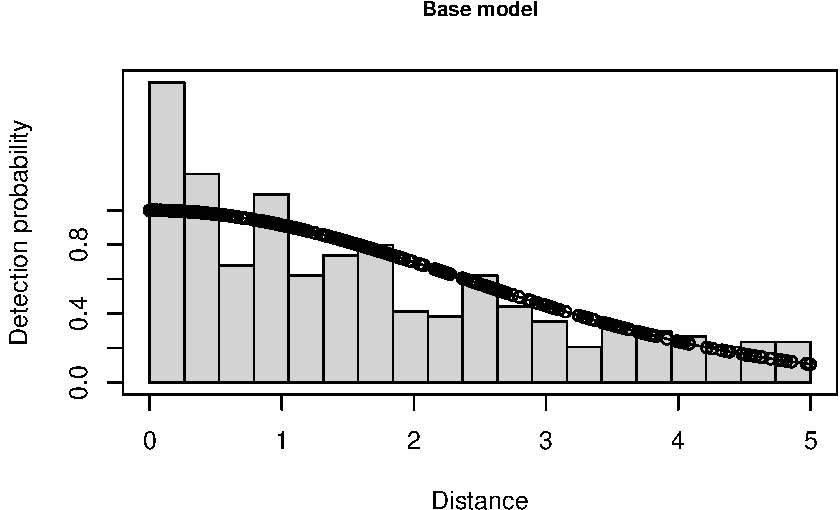
\includegraphics{figures/unnamed-chunk-177-2.pdf}

\begin{verbatim}
Error in create.model.frame(xmat, as.formula(ddfobj$scale$formula), meta.data,  : 
  NA covariate values in the data, check your data.
\end{verbatim}

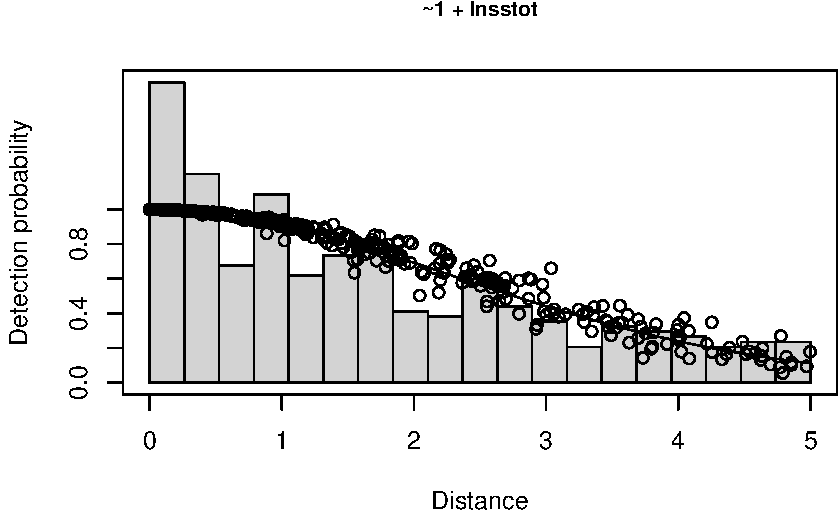
\includegraphics{figures/unnamed-chunk-177-3.pdf} 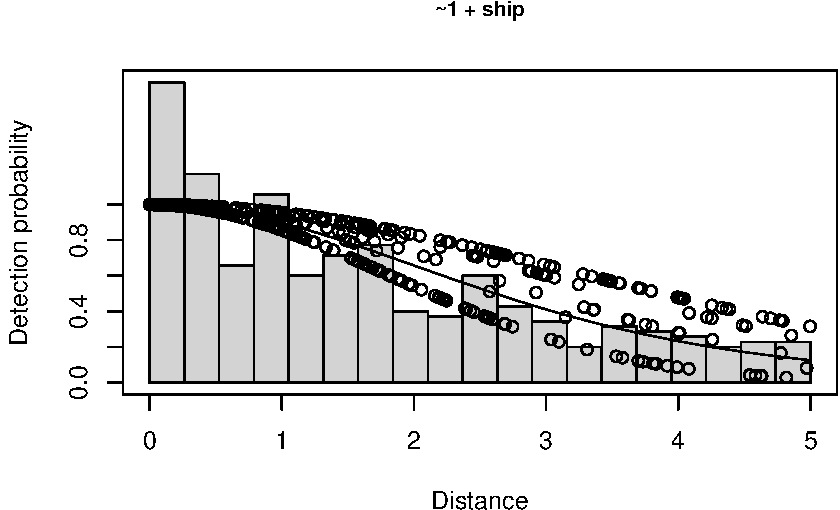
\includegraphics{figures/unnamed-chunk-177-4.pdf} 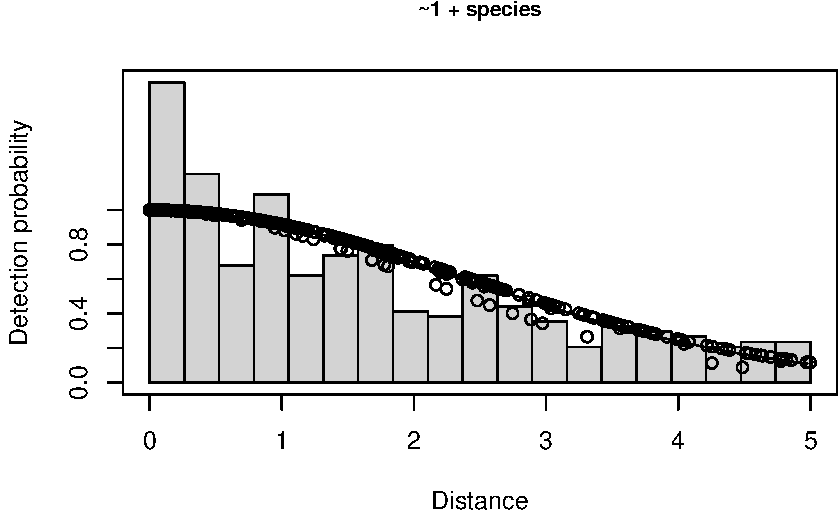
\includegraphics{figures/unnamed-chunk-177-5.pdf}

\begin{verbatim}
Error in create.model.frame(xmat, as.formula(ddfobj$scale$formula), meta.data,  : 
  NA covariate values in the data, check your data.
\end{verbatim}

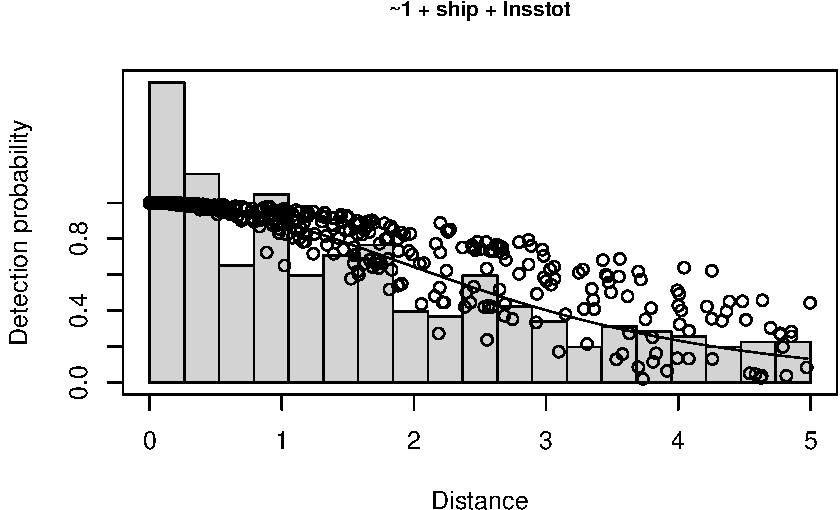
\includegraphics{figures/unnamed-chunk-177-6.pdf} 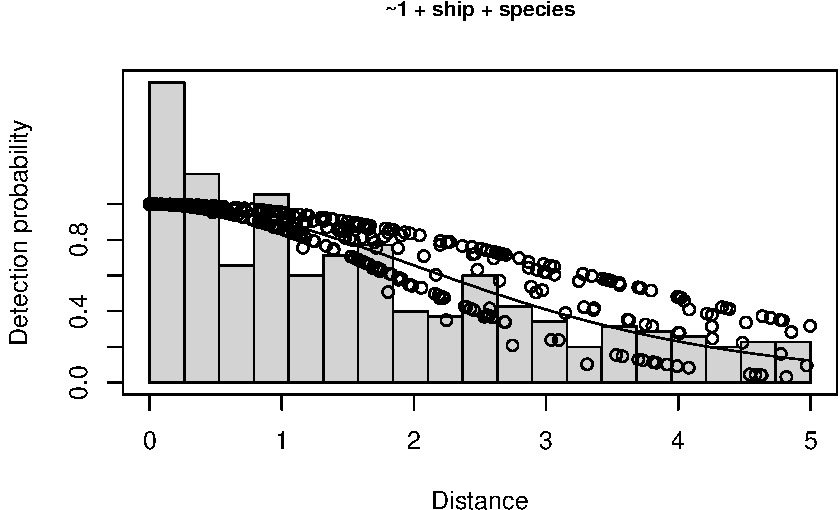
\includegraphics{figures/unnamed-chunk-177-7.pdf}

\begin{verbatim}
Error in create.model.frame(xmat, as.formula(ddfobj$scale$formula), meta.data,  : 
  NA covariate values in the data, check your data.
\end{verbatim}

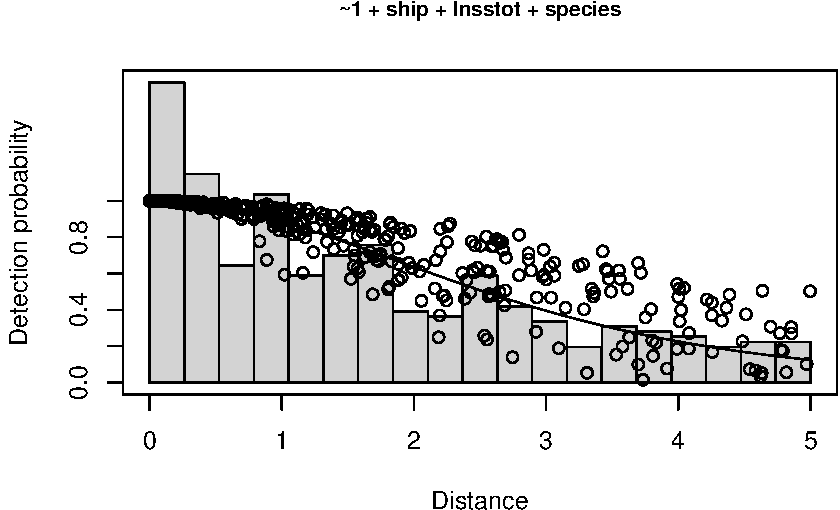
\includegraphics{figures/unnamed-chunk-177-8.pdf}

\begin{verbatim}
Error in View(estimate_results, title = "Abundance") : 
  invalid 'x' argument
\end{verbatim}

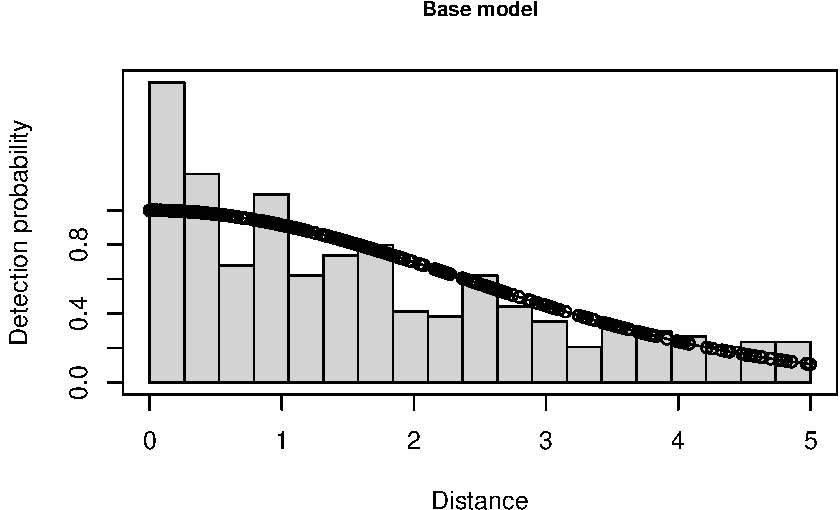
\includegraphics{figures/unnamed-chunk-177-9.pdf}

\begin{verbatim}
Error in create.model.frame(xmat, as.formula(ddfobj$scale$formula), meta.data,  : 
  NA covariate values in the data, check your data.
\end{verbatim}

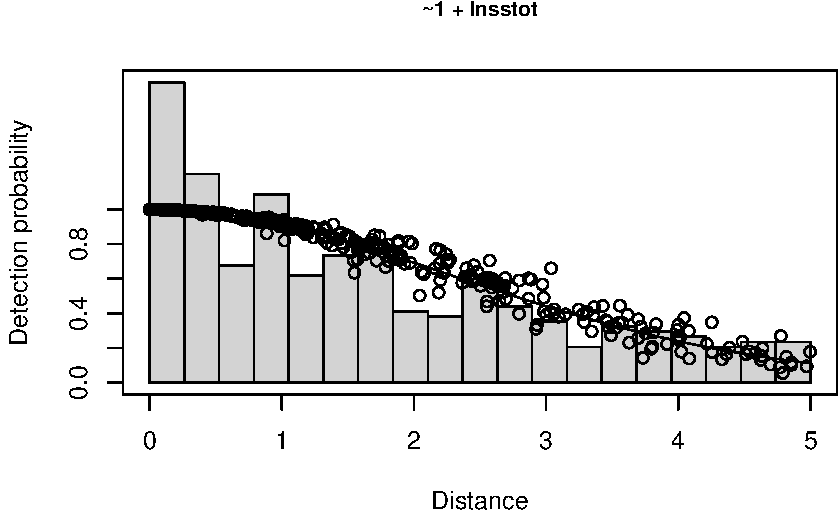
\includegraphics{figures/unnamed-chunk-177-10.pdf} 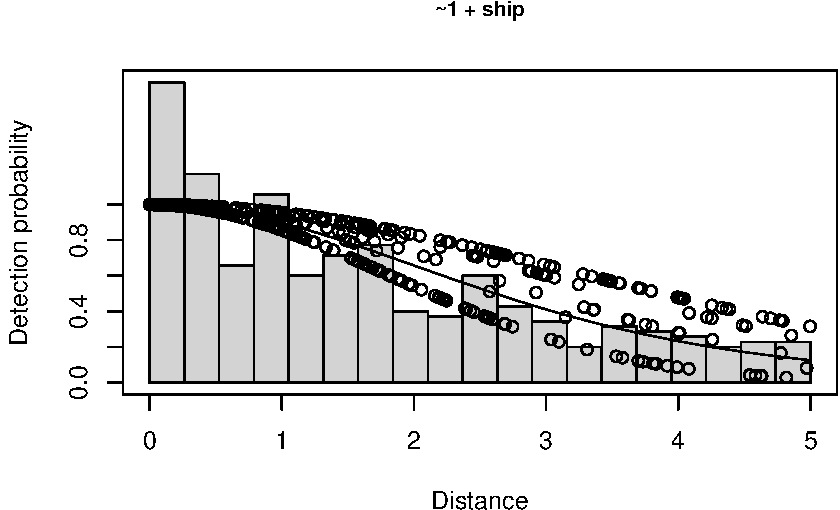
\includegraphics{figures/unnamed-chunk-177-11.pdf} 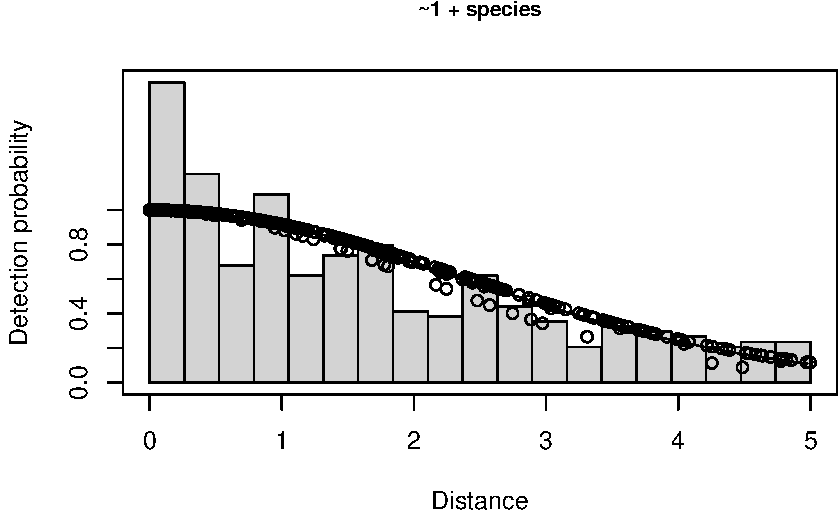
\includegraphics{figures/unnamed-chunk-177-12.pdf}

\begin{verbatim}
Error in create.model.frame(xmat, as.formula(ddfobj$scale$formula), meta.data,  : 
  NA covariate values in the data, check your data.
\end{verbatim}

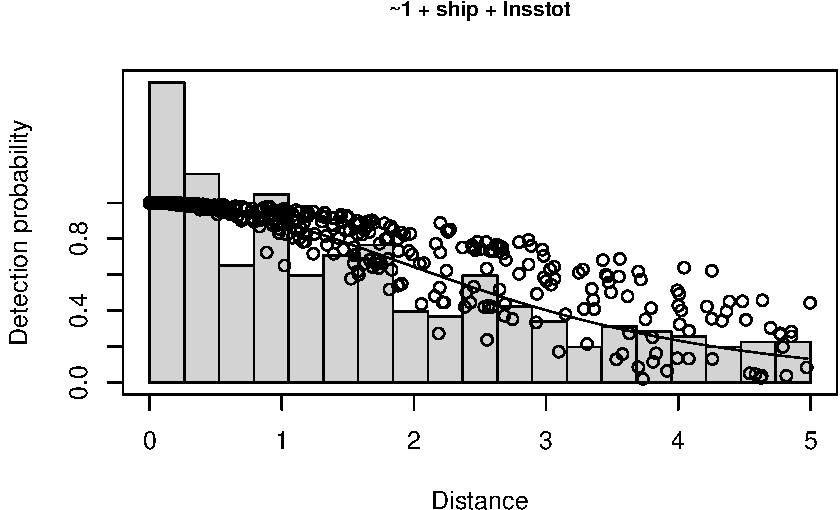
\includegraphics{figures/unnamed-chunk-177-13.pdf} 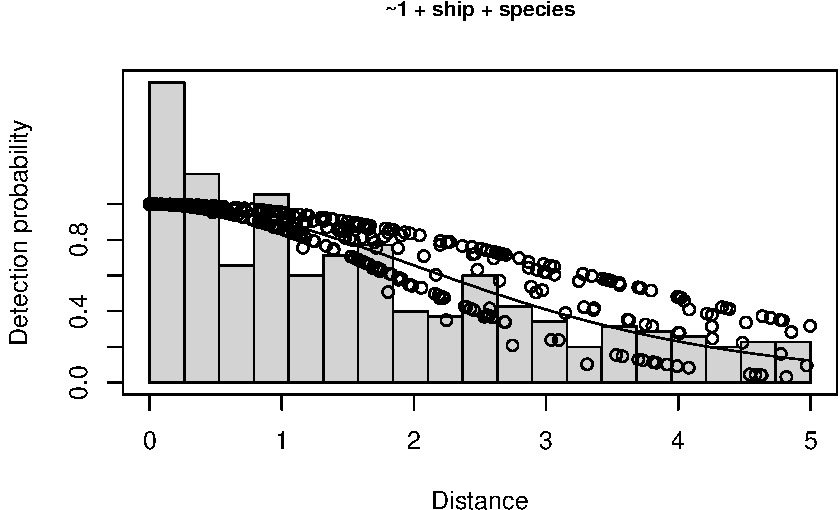
\includegraphics{figures/unnamed-chunk-177-14.pdf}

\begin{verbatim}
Error in create.model.frame(xmat, as.formula(ddfobj$scale$formula), meta.data,  : 
  NA covariate values in the data, check your data.
\end{verbatim}

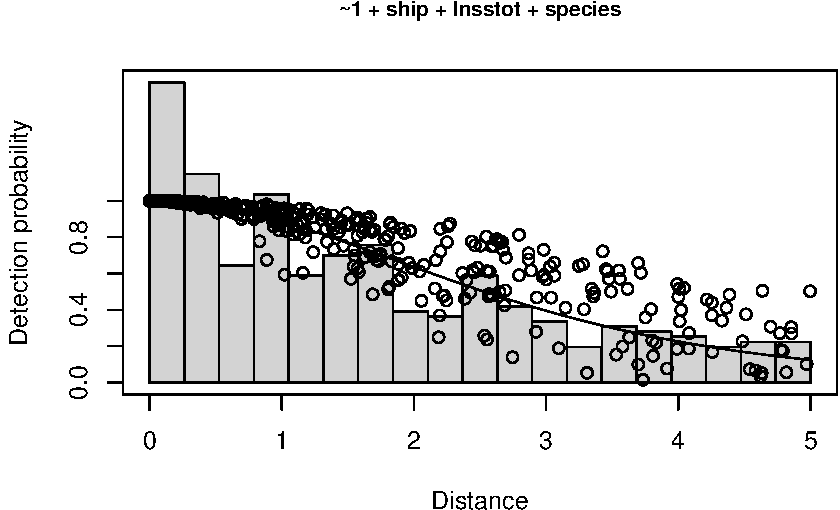
\includegraphics{figures/unnamed-chunk-177-15.pdf}

\begin{verbatim}
Error in View(estimate_results, title = "Abundance") : 
  invalid 'x' argument
\end{verbatim}

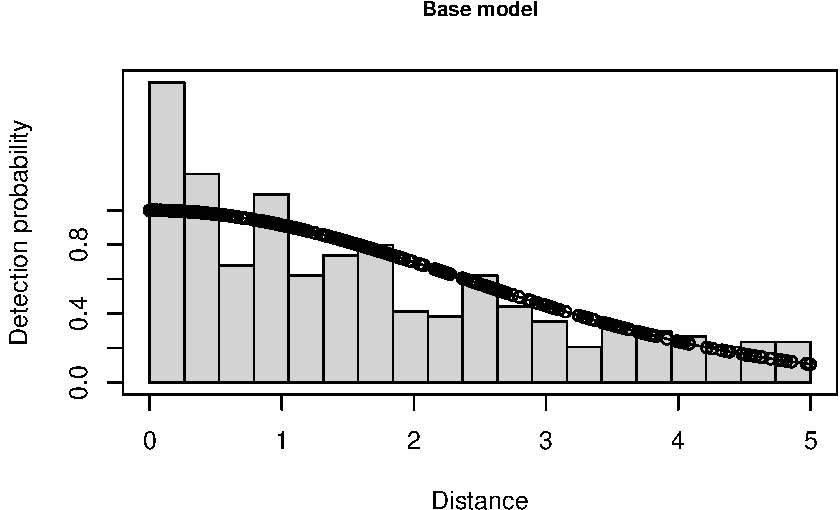
\includegraphics{figures/unnamed-chunk-177-16.pdf}

\begin{verbatim}
Error in create.model.frame(xmat, as.formula(ddfobj$scale$formula), meta.data,  : 
  NA covariate values in the data, check your data.
\end{verbatim}

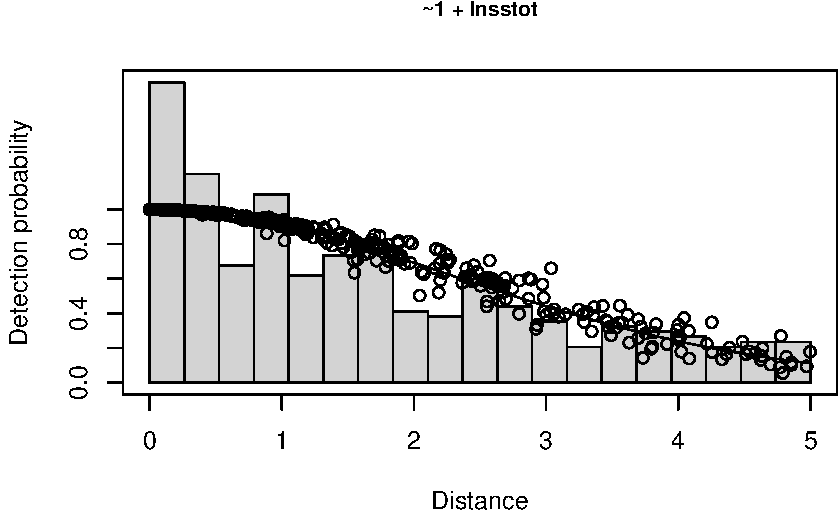
\includegraphics{figures/unnamed-chunk-177-17.pdf} 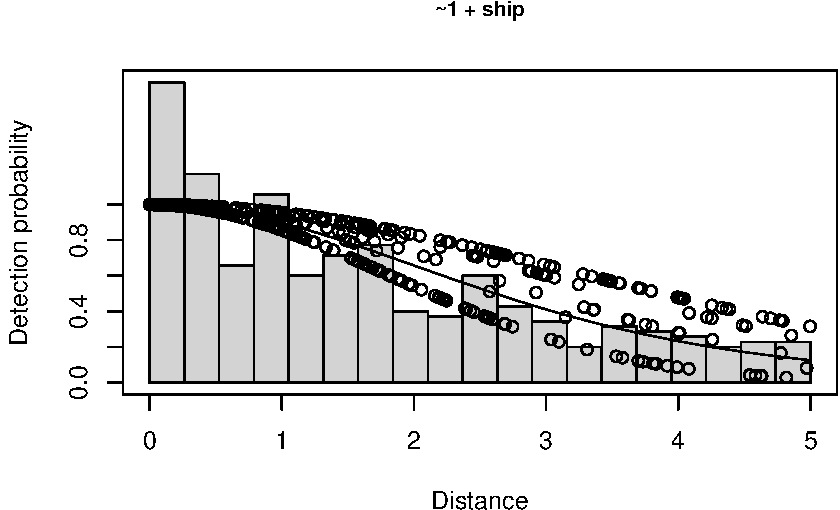
\includegraphics{figures/unnamed-chunk-177-18.pdf} 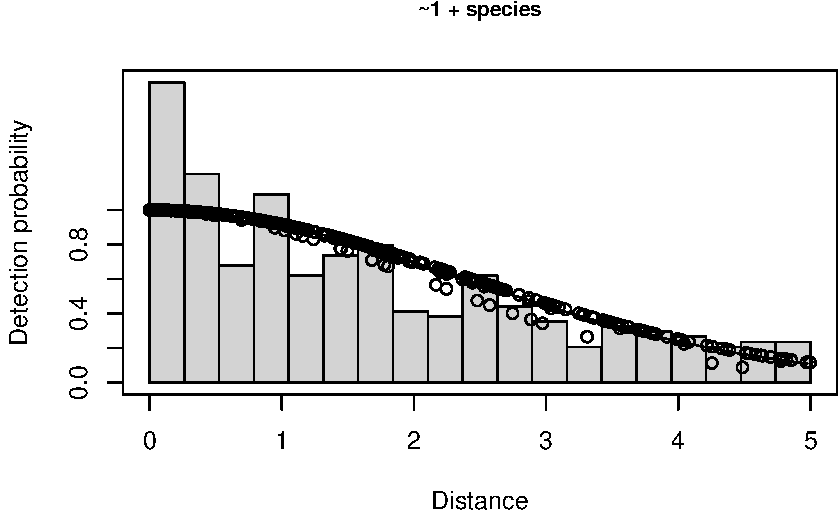
\includegraphics{figures/unnamed-chunk-177-19.pdf}

\begin{verbatim}
Error in create.model.frame(xmat, as.formula(ddfobj$scale$formula), meta.data,  : 
  NA covariate values in the data, check your data.
\end{verbatim}

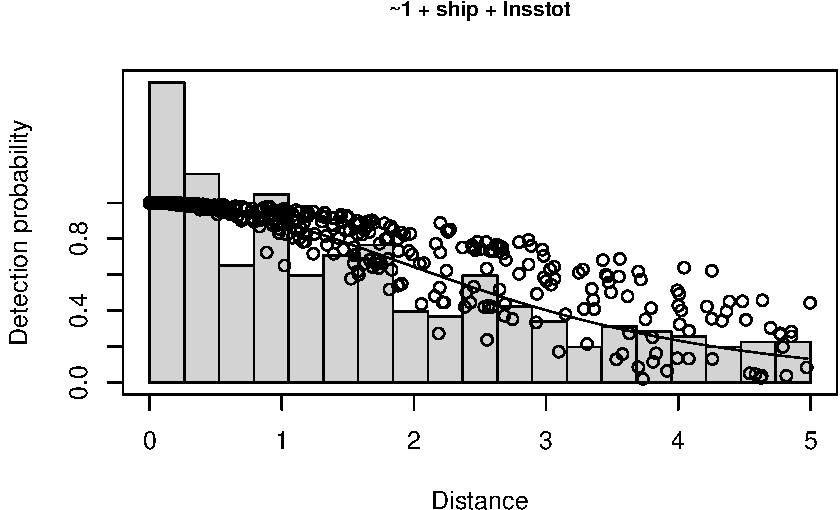
\includegraphics{figures/unnamed-chunk-177-20.pdf} 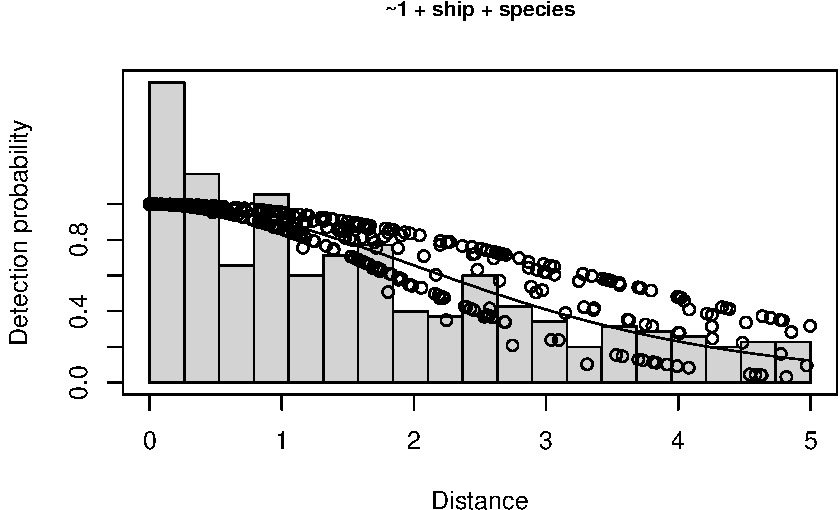
\includegraphics{figures/unnamed-chunk-177-21.pdf}

\begin{verbatim}
Error in create.model.frame(xmat, as.formula(ddfobj$scale$formula), meta.data,  : 
  NA covariate values in the data, check your data.
\end{verbatim}

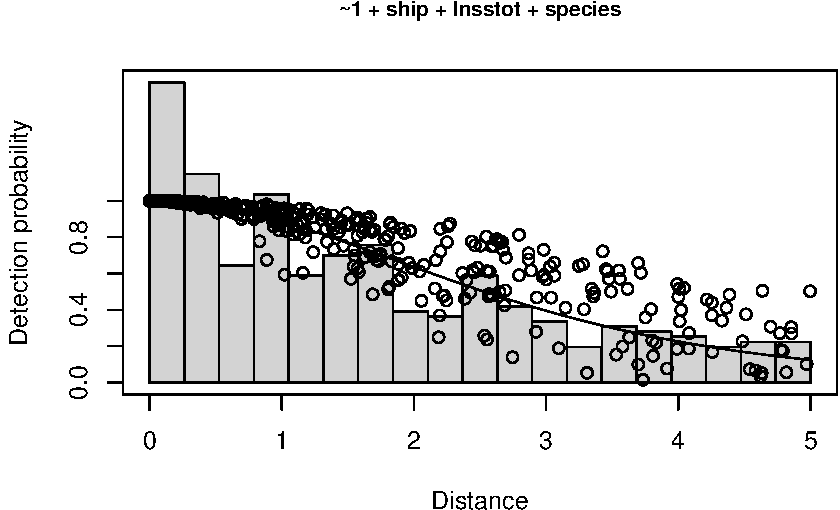
\includegraphics{figures/unnamed-chunk-177-22.pdf}

\begin{verbatim}
Error in View(estimate_results, title = "Abundance") : 
  invalid 'x' argument
\end{verbatim}

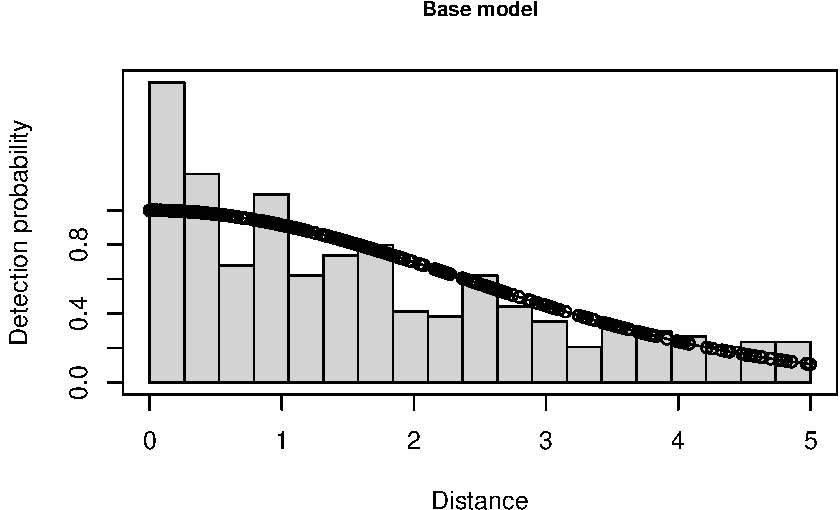
\includegraphics{figures/unnamed-chunk-177-23.pdf}

\begin{verbatim}
Error in create.model.frame(xmat, as.formula(ddfobj$scale$formula), meta.data,  : 
  NA covariate values in the data, check your data.
\end{verbatim}

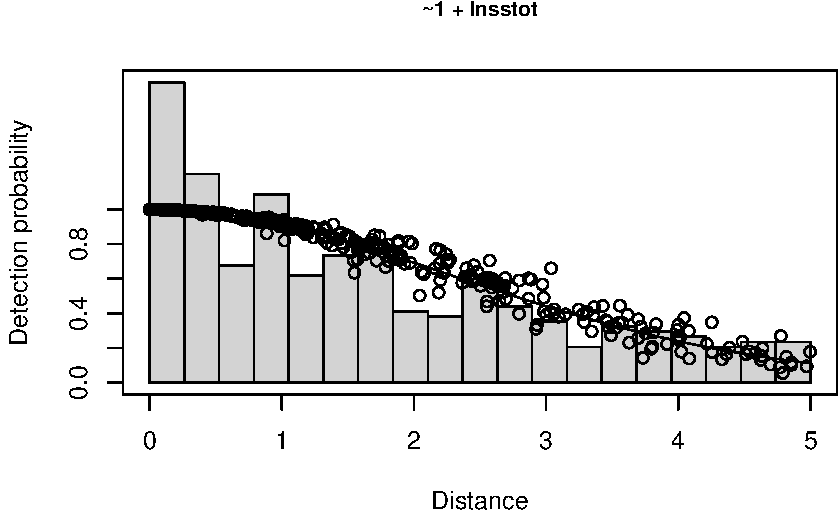
\includegraphics{figures/unnamed-chunk-177-24.pdf} 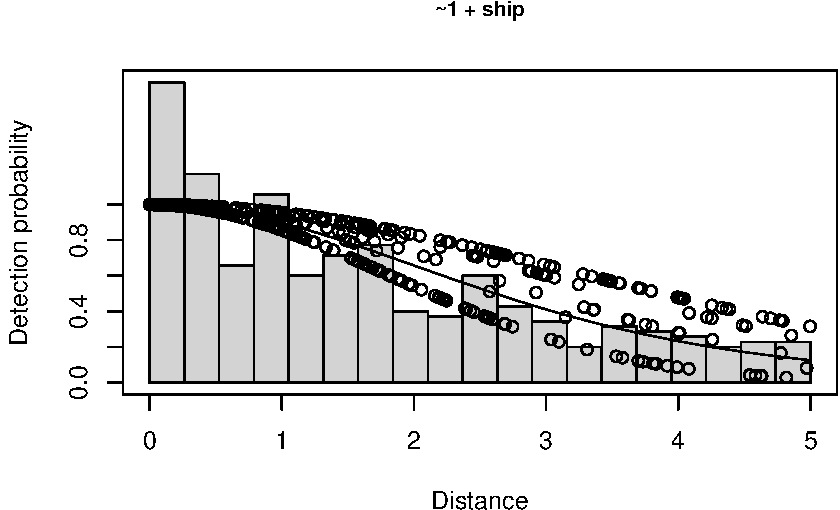
\includegraphics{figures/unnamed-chunk-177-25.pdf} 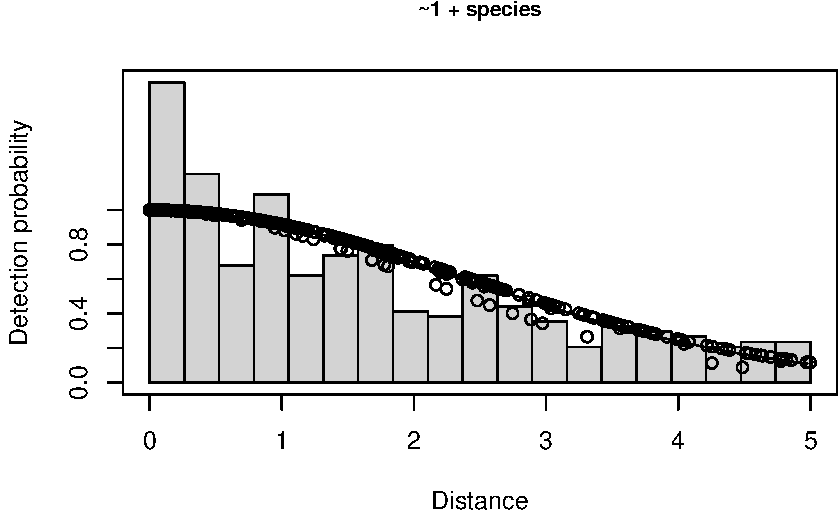
\includegraphics{figures/unnamed-chunk-177-26.pdf}

\begin{verbatim}
Error in create.model.frame(xmat, as.formula(ddfobj$scale$formula), meta.data,  : 
  NA covariate values in the data, check your data.
\end{verbatim}

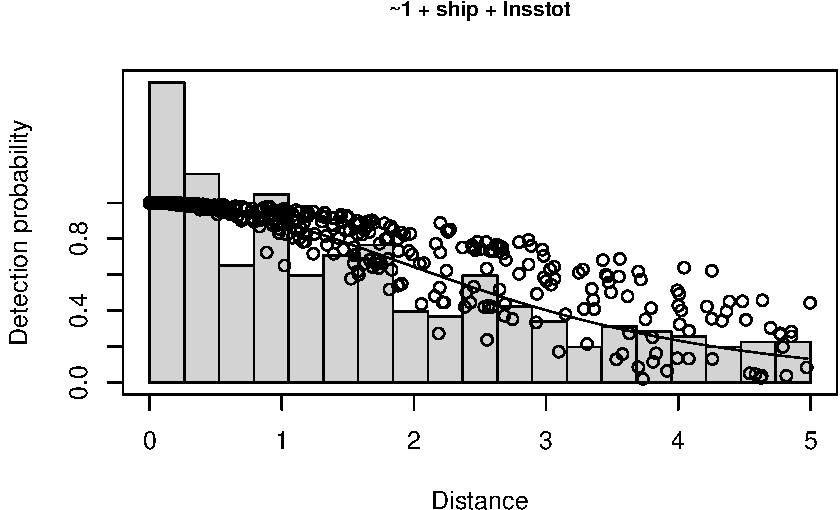
\includegraphics{figures/unnamed-chunk-177-27.pdf} 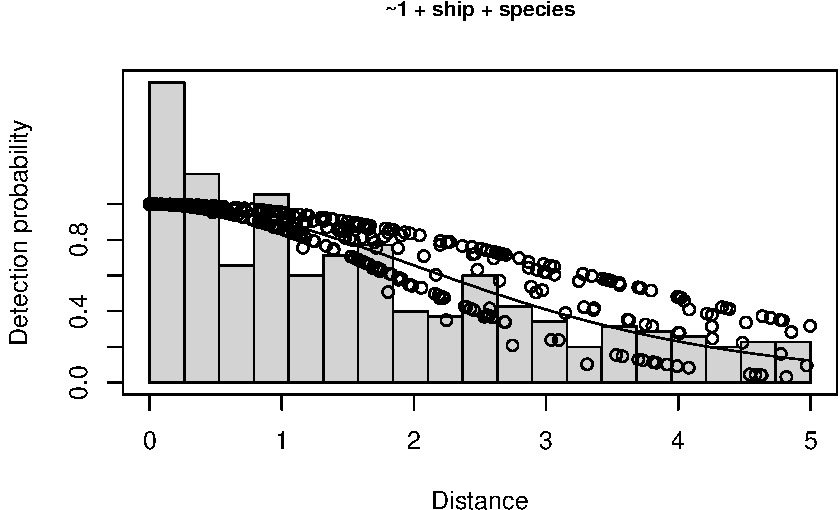
\includegraphics{figures/unnamed-chunk-177-28.pdf}

\begin{verbatim}
Error in create.model.frame(xmat, as.formula(ddfobj$scale$formula), meta.data,  : 
  NA covariate values in the data, check your data.
Error in View(estimate_results, title = "Abundance") : 
  invalid 'x' argument
Error in lta(cruz, Rg0, fit_filters, df_settings, new_estimates): Three failed attempts to complete the analysis for this iteration!
\end{verbatim}

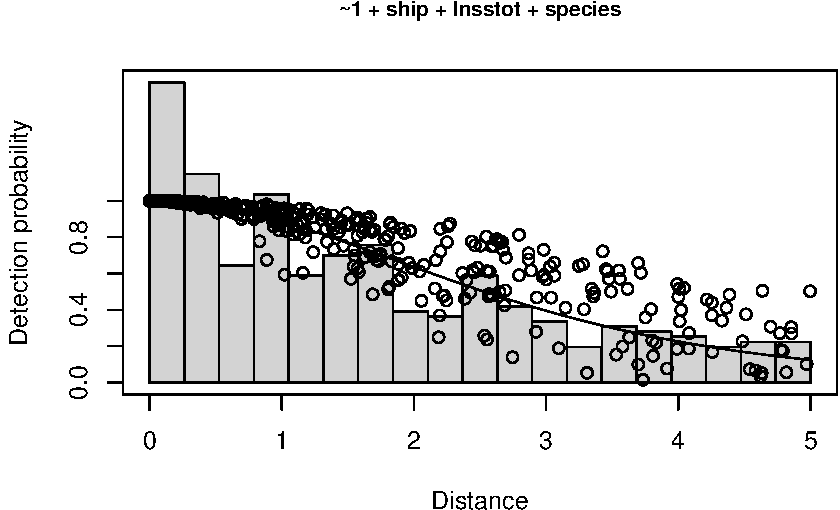
\includegraphics{figures/unnamed-chunk-177-29.pdf}

Additionally, windows will appear showing details for the detection function models and details of the density/abundance estimate.

\hypertarget{outputs}{%
\subsection*{Outputs}\label{outputs}}
\addcontentsline{toc}{subsection}{Outputs}

The \texttt{lta()} function returns a list of objects. To demonstrate this output, we will pull back in the dataset representing the result of the analysis above, for all three species in both years (with 5 bootstrap iterations):

This list of results has five slots:

\begin{Shaded}
\begin{Highlighting}[]
\KeywordTok{names}\NormalTok{(results)}
\NormalTok{[}\DecValTok{1}\NormalTok{] }\StringTok{"pool"}      \StringTok{"inputs"}    \StringTok{"estimate"}  \StringTok{"df"}        \StringTok{"bootstrap"}
\end{Highlighting}
\end{Shaded}

\begin{enumerate}
\def\labelenumi{(\arabic{enumi})}
\item
  \textbf{\texttt{pool}}: The species pool pertaining to these estimates.
\item
  \textbf{\texttt{inputs}}: A list of the inputs used to produce these estimates.
\item
  \textbf{\texttt{estimate}}: A table of density/abundance estimates for each species/region/year combination specified in the \texttt{estimates} input.
\end{enumerate}

\begin{Shaded}
\begin{Highlighting}[]
\NormalTok{results}\OperatorTok{$}\NormalTok{estimate}
\NormalTok{               title species    Region     Area year segments       km}
\DecValTok{1}\NormalTok{    Striped dolphin     }\DecValTok{013}\NormalTok{ (WHICEAS) }\FloatTok{402948.7} \DecValTok{2017}       \DecValTok{38} \FloatTok{3040.009}
\DecValTok{2}\NormalTok{    Striped dolphin     }\DecValTok{013}\NormalTok{ (WHICEAS) }\FloatTok{402948.7} \DecValTok{2020}       \DecValTok{40} \FloatTok{4585.386}
\DecValTok{3}\NormalTok{    Frasers dolphin     }\DecValTok{026}\NormalTok{ (WHICEAS) }\FloatTok{402948.7} \DecValTok{2020}       \DecValTok{40} \FloatTok{4585.386}
\DecValTok{4}\NormalTok{ Melon}\OperatorTok{-}\NormalTok{headed whale     }\DecValTok{031}\NormalTok{ (WHICEAS) }\FloatTok{402948.7} \DecValTok{2017}       \DecValTok{38} \FloatTok{3040.009}
\DecValTok{5}\NormalTok{ Melon}\OperatorTok{-}\NormalTok{headed whale     }\DecValTok{031}\NormalTok{ (WHICEAS) }\FloatTok{402948.7} \DecValTok{2020}       \DecValTok{40} \FloatTok{4585.386}
\NormalTok{  Area_covered ESW_mean n g0_est  ER_clusters   D_clusters N_clusters size_mean}
\DecValTok{1}      \FloatTok{9610.88} \FloatTok{3.161465} \DecValTok{3}  \FloatTok{0.316} \FloatTok{0.0009868393} \FloatTok{0.0005004327}  \FloatTok{201.64872}  \FloatTok{31.95079}
\DecValTok{2}     \FloatTok{16236.27} \FloatTok{3.540874} \DecValTok{3}  \FloatTok{0.280} \FloatTok{0.0006542525} \FloatTok{0.0003299532}  \FloatTok{132.95423}  \FloatTok{53.95865}
\DecValTok{3}     \FloatTok{17084.73} \FloatTok{3.725909} \DecValTok{2}  \FloatTok{0.448} \FloatTok{0.0004361683} \FloatTok{0.0001306527}   \FloatTok{52.64635} \FloatTok{132.51143}
\DecValTok{4}     \FloatTok{10669.12} \FloatTok{3.509569} \DecValTok{2}  \FloatTok{0.509} \FloatTok{0.0006578929} \FloatTok{0.0001842793}   \FloatTok{74.25510} \FloatTok{185.98103}
\DecValTok{5}     \FloatTok{16949.65} \FloatTok{3.696451} \DecValTok{3}  \FloatTok{0.483} \FloatTok{0.0006542525} \FloatTok{0.0001832491}   \FloatTok{73.84001} \FloatTok{226.13289}
\NormalTok{      size_sd         ER          D         N}
\DecValTok{1}   \FloatTok{0.5780968} \FloatTok{0.03153029} \FloatTok{0.01601708}  \FloatTok{6454.061}
\DecValTok{2}   \FloatTok{2.7402089} \FloatTok{0.03530258} \FloatTok{0.01780121}  \FloatTok{7172.977}
\DecValTok{3} \FloatTok{182.1747087} \FloatTok{0.05779729} \FloatTok{0.01725827}  \FloatTok{6954.200}
\DecValTok{4}  \FloatTok{96.4369707} \FloatTok{0.12235559} \FloatTok{0.03392990} \FloatTok{13672.011}
\DecValTok{5} \FloatTok{175.5620746} \FloatTok{0.14794801} \FloatTok{0.04158955} \FloatTok{16758.457}
\end{Highlighting}
\end{Shaded}

\begin{enumerate}
\def\labelenumi{(\arabic{enumi})}
\setcounter{enumi}{3}
\tightlist
\item
  \textbf{\texttt{df}}: A named list with details for the detection function.
\end{enumerate}

\begin{Shaded}
\begin{Highlighting}[]
\NormalTok{results}\OperatorTok{$}\NormalTok{df }\OperatorTok\StringTok{ }\NormalTok{names}
\NormalTok{[}\DecValTok{1}\NormalTok{] }\StringTok{"best_models"}  \StringTok{"all_models"}   \StringTok{"best_objects"} \StringTok{"sightings"}    \StringTok{"sample_size"} 
\NormalTok{[}\DecValTok{6}\NormalTok{] }\StringTok{"curve"}       

\NormalTok{results}\OperatorTok{$}\NormalTok{df}\OperatorTok{$}\NormalTok{best_models}
\NormalTok{  Model Key_function                       Formula     Pmean      AIC}
\DecValTok{1}     \DecValTok{5}\NormalTok{           hn           }\OperatorTok{~}\DecValTok{1} \OperatorTok{+}\StringTok{ }\NormalTok{ship }\OperatorTok{+}\StringTok{ }\NormalTok{lnsstot }\FloatTok{0.5481587} \FloatTok{1058.131}
\DecValTok{2}     \DecValTok{7}\NormalTok{           hn }\OperatorTok{~}\DecValTok{1} \OperatorTok{+}\StringTok{ }\NormalTok{ship }\OperatorTok{+}\StringTok{ }\NormalTok{lnsstot }\OperatorTok{+}\StringTok{ }\NormalTok{species }\FloatTok{0.5422751} \FloatTok{1058.232}
  \OperatorTok{$}\NormalTok{\textbackslash{}\textbackslash{}Delta}\OperatorTok{$}\NormalTok{AIC           Covariates tested                 pool}
\DecValTok{1}        \FloatTok{0.000}\NormalTok{ bft, lnsstot, ship, species Multi}\OperatorTok{-}\NormalTok{species pool }\DecValTok{1}
\DecValTok{2}        \FloatTok{0.101}\NormalTok{ bft, lnsstot, ship, species Multi}\OperatorTok{-}\NormalTok{species pool }\DecValTok{1}
\end{Highlighting}
\end{Shaded}

\begin{enumerate}
\def\labelenumi{(\arabic{enumi})}
\setcounter{enumi}{4}
\tightlist
\item
  \textbf{\texttt{bootstrap}}: If bootstrap variance estimation was carried out, the output would also include \texttt{bootstrap}, a named list with results from the bootstrap process, only returned if the bootstraps input is greater than 1.
\end{enumerate}

\begin{Shaded}
\begin{Highlighting}[]
\NormalTok{results}\OperatorTok{$}\NormalTok{bootstrap }\OperatorTok\StringTok{ }\NormalTok{names}
\NormalTok{[}\DecValTok{1}\NormalTok{] }\StringTok{"summary"} \StringTok{"details"} \StringTok{"df"}     
\end{Highlighting}
\end{Shaded}

\begin{Shaded}
\begin{Highlighting}[]
\NormalTok{results}\OperatorTok{$}\NormalTok{bootstrap}\OperatorTok{$}\NormalTok{summary }\OperatorTok\StringTok{ }\NormalTok{head}
\CommentTok{# A tibble: 5 x 18}
\CommentTok{# Groups:   title, Region [3]}
\NormalTok{  title      Region year  species iterations ESW_mean g0_mean g0_cv    km     ER}
  \OperatorTok{<}\NormalTok{chr}\OperatorTok{>}\StringTok{      }\ErrorTok{<}\NormalTok{chr}\OperatorTok{>}\StringTok{  }\ErrorTok{<}\NormalTok{chr}\OperatorTok{>}\StringTok{ }\ErrorTok{<}\NormalTok{chr}\OperatorTok{>}\StringTok{        }\ErrorTok{<}\NormalTok{int}\OperatorTok{>}\StringTok{    }\ErrorTok{<}\NormalTok{dbl}\OperatorTok{>}\StringTok{   }\ErrorTok{<}\NormalTok{dbl}\OperatorTok{>}\StringTok{ }\ErrorTok{<}\NormalTok{dbl}\OperatorTok{>}\StringTok{ }\ErrorTok{<}\NormalTok{dbl}\OperatorTok{>}\StringTok{  }\ErrorTok{<}\NormalTok{dbl}\OperatorTok{>}
\DecValTok{1}\NormalTok{ Frasers d}\OperatorTok{~}\StringTok{ }\NormalTok{(WHIC}\OperatorTok{~}\StringTok{ }\DecValTok{2020}  \DecValTok{026}             \DecValTok{10}     \FloatTok{3.59}   \FloatTok{0.451} \FloatTok{0.864} \FloatTok{4512.} \FloatTok{0.105} 
\DecValTok{2}\NormalTok{ Melon}\OperatorTok{-}\NormalTok{hea}\OperatorTok{~}\StringTok{ }\NormalTok{(WHIC}\OperatorTok{~}\StringTok{ }\DecValTok{2017}  \DecValTok{031}             \DecValTok{10}     \FloatTok{3.36}   \FloatTok{0.393} \FloatTok{0.816} \FloatTok{3133.} \FloatTok{0.153} 
\DecValTok{3}\NormalTok{ Melon}\OperatorTok{-}\NormalTok{hea}\OperatorTok{~}\StringTok{ }\NormalTok{(WHIC}\OperatorTok{~}\StringTok{ }\DecValTok{2020}  \DecValTok{031}             \DecValTok{10}     \FloatTok{3.54}   \FloatTok{0.544} \FloatTok{0.678} \FloatTok{4512.} \FloatTok{0.179} 
\DecValTok{4}\NormalTok{ Striped d}\OperatorTok{~}\StringTok{ }\NormalTok{(WHIC}\OperatorTok{~}\StringTok{ }\DecValTok{2017}  \DecValTok{013}             \DecValTok{10}     \FloatTok{3.34}   \FloatTok{0.313} \FloatTok{0.150} \FloatTok{3133.} \FloatTok{0.0488}
\DecValTok{5}\NormalTok{ Striped d}\OperatorTok{~}\StringTok{ }\NormalTok{(WHIC}\OperatorTok{~}\StringTok{ }\DecValTok{2020}  \DecValTok{013}             \DecValTok{10}     \FloatTok{3.58}   \FloatTok{0.277} \FloatTok{0.128} \FloatTok{4512.} \FloatTok{0.0493}
\CommentTok{# ... with 8 more variables: D <dbl>, size <dbl>, Nmean <dbl>, Nmedian <dbl>,}
\CommentTok{#   Nsd <dbl>, CV <dbl>, L95 <dbl>, U95 <dbl>}
\end{Highlighting}
\end{Shaded}

\hypertarget{unusual-estimate-scenarios}{%
\section*{Unusual estimate scenarios}\label{unusual-estimate-scenarios}}
\addcontentsline{toc}{section}{Unusual estimate scenarios}

Most line-transect estimates in most areas are relatively straightforward: you want an estimate for a single species in a single year, and your geostrata do not overlap, nor do they need to be stratified or combined in funny ways.

But there will also be unusual and slightly more complicated scenarios. We outline some of those below and demonstrate how they can be handled within the \texttt{LTabundR} framework.

\hypertarget{species-combinations-g0}{%
\subsection*{\texorpdfstring{Species combinations \& \emph{g(0)}}{Species combinations \& g(0)}}\label{species-combinations-g0}}
\addcontentsline{toc}{subsection}{Species combinations \& \emph{g(0)}}

\hypertarget{multi-species-schools}{%
\subsubsection*{Multi-species schools}\label{multi-species-schools}}
\addcontentsline{toc}{subsubsection}{Multi-species schools}

Multi-species schools can confound detection function model fitting, since your species of interest may not be the predominant species in the group, which means that the other species present may be having a greater influence over the detection function. You can decide how to account for this using the \texttt{other\_species} slot in your \texttt{fit\_filters} list. See the details on this discussed above.

\hypertarget{species-pools}{%
\subsubsection*{Species pools}\label{species-pools}}
\addcontentsline{toc}{subsubsection}{Species pools}

When you don't have enough sightings of individual species to model a detection function effectively, it can be useful to pool sightings from multiple species who have similar detection characteristics. This is a common tactic in the Central North Pacific.

When you do this, you typically need to make the following changes to a ``normal'' \texttt{lta()} call:

\begin{enumerate}
\def\labelenumi{(\arabic{enumi})}
\item
  In your \texttt{df\_settings} list, consider adding \texttt{species} as a covariate, and ensure that you specify that it should be treated as a factor. This may improve detection function model fit.
\item
  In your \texttt{fit\_filters} list, specify multiple species codes and name your species pool accordingly (e.g., ``Multi-species pool 1'').
\item
  In your \texttt{fit\_filters} list, specify how to handle ``Other'' species (see above).
\item
  In your \texttt{estimates} list, add a sub-list for each species-region-year for which you want a density/abundance estimate.
\end{enumerate}

We took all of these steps in the example above with striped dolphins, Fraser's dolphins, and melon-headed whales. Use that code as a guide.

\hypertarget{pooling-similar-species}{%
\subsubsection*{Pooling similar species}\label{pooling-similar-species}}
\addcontentsline{toc}{subsubsection}{Pooling similar species}

Species that can be confused with one another may need to be pooled together for abundance estimation. For example, in the northeast Pacific, sei whales, Bryde's whales, and fin whales can co-occur but they are difficult to distinguish in the field. They are also relatively uncommon, and may need to be pooled with other species in order to obtain a sound detection function model. To account for this, we want to estimate the density/abundance in the WHICEAS study area of all detections of sei, Bryde's, fin whales together.

To handle this, we will follow all the steps taken for a multi-species pool, as discussed above. Additionally, in our \texttt{estimates} sub-list(s), we will specify (1) that multiple species should be included in the estimate, and (2) that the weighted \emph{g(0)} estimates for each of the individual species should be averaged together:

\begin{Shaded}
\begin{Highlighting}[]
\NormalTok{estimates <-}\StringTok{ }\KeywordTok{list}\NormalTok{(}
  \KeywordTok{list}\NormalTok{(}\DataTypeTok{spp =} \KeywordTok{c}\NormalTok{(}\StringTok{'072'}\NormalTok{, }\StringTok{'073'}\NormalTok{, }\StringTok{'099'}\NormalTok{, }\StringTok{'074'}\NormalTok{),}
       \DataTypeTok{title =} \StringTok{"Sei/Bryde's/Fin whale"}\NormalTok{,}
       \DataTypeTok{years =} \DecValTok{2017}\NormalTok{,}
       \DataTypeTok{regions =} \StringTok{'WHICEAS'}\NormalTok{,}
       \DataTypeTok{combine_g0 =} \OtherTok{TRUE}\NormalTok{))}
\end{Highlighting}
\end{Shaded}

\hypertarget{rare-unidentified-taxa}{%
\subsubsection*{Rare unidentified taxa}\label{rare-unidentified-taxa}}
\addcontentsline{toc}{subsubsection}{Rare unidentified taxa}

A similar problem occur when you have species codes for unidentified taxa that have been identified down to a family- or genus-level. For example, ``Unidenfitied \emph{Mesoplodon}'' is a species code (the code is \texttt{"050"}) for any beaked whale that is definitely in the genus \emph{Mesoplodon}. There are plenty of these sightings, which means \emph{g(0)} and its CV can be estimated just fine without referring to other species codes.

Other unidentified taxa, however, are less common. For example, in Hawaiian studies, density/abundance is estimated for ``Unidentified rorquals''. In the field there is a species code for this group, \texttt{"070"}, but it is rarely used -- there are enough sightings to model the detection function, but not nearly enough sightings to estimate \emph{g(0)} or its CV. In this case, we need to combine \emph{g(0)} from more common species codes in order to estimate the unidentified rorqual's \emph{g(0)}.

To do this, we fit a detection function using species code \texttt{"070"} \ldots{}

\begin{Shaded}
\begin{Highlighting}[]
\NormalTok{fit_filters <-}
\StringTok{    }\KeywordTok{list}\NormalTok{(}\DataTypeTok{spp =} \KeywordTok{c}\NormalTok{(}\StringTok{'070'}\NormalTok{),}
         \DataTypeTok{pool =} \StringTok{'Unidentified rorqual'}\NormalTok{,}
         \DataTypeTok{cohort =} \StringTok{'all'}\NormalTok{,}
         \DataTypeTok{truncation_distance =} \FloatTok{5.5}\NormalTok{)}
\end{Highlighting}
\end{Shaded}

\ldots{} then, in our \texttt{estimates} list, we specify some alternate \texttt{g(0)} species designations.

\begin{Shaded}
\begin{Highlighting}[]
\NormalTok{estimates <-}\StringTok{ }\KeywordTok{list}\NormalTok{(}
    \KeywordTok{list}\NormalTok{(}\DataTypeTok{spp =} \StringTok{'070'}\NormalTok{,}
         \DataTypeTok{title =} \StringTok{'Unidentified rorqual'}\NormalTok{,}
         \DataTypeTok{years =} \DecValTok{2017}\NormalTok{,}
         \DataTypeTok{regions =} \StringTok{'WHICEAS'}\NormalTok{,}
         \DataTypeTok{alt_g0_spp =} \KeywordTok{c}\NormalTok{(}\StringTok{'071'}\NormalTok{,}\StringTok{'099'}\NormalTok{,}\StringTok{'074'}\NormalTok{,}\StringTok{'075'}\NormalTok{),}
         \DataTypeTok{combine_g0 =} \OtherTok{TRUE}\NormalTok{))}
\end{Highlighting}
\end{Shaded}

\hypertarget{geostratum-combinations}{%
\subsection*{Geostratum combinations}\label{geostratum-combinations}}
\addcontentsline{toc}{subsection}{Geostratum combinations}

In your \texttt{estimates} sub-lists, the \texttt{regions} and \texttt{regions\_remove} slots give you control of the geographic scope of (1) the weighted \emph{g(0)} and CV used in density estimation, (2) the effort and sightings used to estimate density, (3) and the area used to calculate abundance.

\hypertarget{a-note-on-cohort-geostrata}{%
\subsubsection*{A note on cohort geostrata}\label{a-note-on-cohort-geostrata}}
\addcontentsline{toc}{subsubsection}{A note on cohort geostrata}

Recall that, when processing your survey data to create a \texttt{cruz} object, you provide a list of geostrata as an argument in your \texttt{process\_surveys()} call. You also have the option to specify a subset of those geostrata for each species cohort (see \texttt{load\_cohort\_settings()}), which is an option that you should almost always use. Selecting a subset of geostrata is important because that subset is used to ``segmentize'' your survey data -- i.e., break effort into discrete sections that can be bootstrap-sampling during the \texttt{lta()} variance estimation routine -- and the segmentizing procedure always breaks segments when a survey passes from one geostratum to another.

This matters because the \texttt{lta()} bootstrapping routine will re-sample survey segments in a way that preserves the proportion of segments occurring in each geostratum, to ensure that all geostrata are represented in the same proportion as the original estimate. When segments are unncessarily broken into small segments by irrelevant geostrata that have been included in the analysis, the bootstrap estimate of the CV is likely to be too large.

For example: in the Central North Pacific, there are about 11 geostrata commonly used. These include the Hawaiian EEZ geostratum, the Main Hawaiian Islands geostratum, and the larger CNP geostratum that represents the maximum range of the study area. These three geostrata are typically all you need for most density estimates for most species. However, a few species -- e.g., bottlenose dolphin, pantropical spotted dolphin, and false killer whale -- have special geostrata that represent insular stock boundaries and/or pelagic stock boundaries. If those insular geostrata are used in density estimates for which they do not apply, they will confound the bootstrap estimate of density/abundance CV. \textbf{Punchline: be sure to specify only the relevant geostrata in each cohort's settings.}

\hypertarget{combining-disparate-geostrata}{%
\subsubsection*{Combining disparate geostrata}\label{combining-disparate-geostrata}}
\addcontentsline{toc}{subsubsection}{Combining disparate geostrata}

For example, in Hawaii bottlenose dolphins belong to a pelagic stock as well as several insular stocks. If you wished to estimate the abundance of all insular stocks together, you simply provide their respective geostratum names in the \texttt{regions} slot of your \texttt{estimates} sub-list:

\begin{Shaded}
\begin{Highlighting}[]
\NormalTok{estimates <-}\StringTok{ }\KeywordTok{list}\NormalTok{(}\KeywordTok{list}\NormalTok{(}\DataTypeTok{spp =} \StringTok{'018'}\NormalTok{,}
                       \DataTypeTok{title =} \StringTok{'Bottlenose dolphin'}\NormalTok{,}
                       \DataTypeTok{years =} \DecValTok{2017}\NormalTok{,}
                       \DataTypeTok{regions =} \KeywordTok{c}\NormalTok{(}\StringTok{'Bottlenose_KaNi'}\NormalTok{,}
                                   \StringTok{'Bottlenose_OUFI'}\NormalTok{,}
                                   \StringTok{'Bottlenose_BI'}\NormalTok{)))}
\end{Highlighting}
\end{Shaded}

\hypertarget{removing-insular-geostrata}{%
\subsubsection*{Removing insular geostrata}\label{removing-insular-geostrata}}
\addcontentsline{toc}{subsubsection}{Removing insular geostrata}

Conversely, you may wish to estimate density/abundance for \emph{pelagic} bottlenose dolphins only, ignoring the insular stocks. You can substract geostrata using the \texttt{regions\_remove} slot:

\begin{Shaded}
\begin{Highlighting}[]
\NormalTok{estimates <-}\StringTok{ }\KeywordTok{list}\NormalTok{(}\KeywordTok{list}\NormalTok{(}\DataTypeTok{spp =} \StringTok{'018'}\NormalTok{,}
                       \DataTypeTok{title =} \StringTok{'Bottlenose dolphin'}\NormalTok{,}
                       \DataTypeTok{years =} \DecValTok{2017}\NormalTok{,}
                       \DataTypeTok{regions =} \StringTok{'HI_EEZ'}\NormalTok{,}
                       \DataTypeTok{regions_remove =} \KeywordTok{c}\NormalTok{(}\StringTok{'Bottlenose_KaNi'}\NormalTok{,}
                                          \StringTok{'Bottlenose_OUFI'}\NormalTok{,}
                                          \StringTok{'Bottlenose_BI'}\NormalTok{)))}
\end{Highlighting}
\end{Shaded}

\hypertarget{combine-partially-overlapping-geostrata}{%
\subsubsection*{Combine partially overlapping geostrata}\label{combine-partially-overlapping-geostrata}}
\addcontentsline{toc}{subsubsection}{Combine partially overlapping geostrata}

Say you want to estimate the density/abundance for a set of geostrata that partially overlap. An example of this is that the Northwest Hawaiian Islands geostratum overlaps slightly with the Main Hawaiian Islands geostratum. This is not an issue; when study area is calculated within \texttt{lta()} (actually, that function calls another function, \texttt{strata\_area()}, to do this. That function is demonstrated below), overlap among strata is accounted for.

\begin{Shaded}
\begin{Highlighting}[]
\NormalTok{estimates <-}\StringTok{ }\KeywordTok{list}\NormalTok{(}\KeywordTok{list}\NormalTok{(}\DataTypeTok{spp =} \StringTok{'018'}\NormalTok{,}
                       \DataTypeTok{title =} \StringTok{'Bottlenose dolphin'}\NormalTok{,}
                       \DataTypeTok{years =} \DecValTok{2017}\NormalTok{,}
                       \DataTypeTok{regions =} \KeywordTok{c}\NormalTok{(}\StringTok{'MHI'}\NormalTok{,}\StringTok{'NWHI'}\NormalTok{)))}
\end{Highlighting}
\end{Shaded}

\hypertarget{regionally-stratified-analysis}{%
\subsubsection*{Regionally stratified analysis}\label{regionally-stratified-analysis}}
\addcontentsline{toc}{subsubsection}{Regionally stratified analysis}

Field surveys are sometimes stratified such that trackline design and/or density can differ substantially across regions. Also, analysts may sometimes wish to estimate density/abundance for individual regions separately, regardless of design stratification.

In \texttt{lta()}, you can accommodate a stratified analysis by providing an \texttt{estimates} sub-list for each geostratum. For example, in 2002 the Hawaiian EEZ was surveyed with different effort intensity in the Main Hawaiian Islands region compared to pelagic waters. For that reason, density/abundance estimates ought to be stratified by region:

\begin{Shaded}
\begin{Highlighting}[]
\NormalTok{estimates <-}\StringTok{ }\KeywordTok{list}\NormalTok{(}
    \KeywordTok{list}\NormalTok{(}\DataTypeTok{spp =} \StringTok{'013'}\NormalTok{,}
         \DataTypeTok{title =} \StringTok{'Striped dolphin'}\NormalTok{,}
         \DataTypeTok{years =} \DecValTok{2002}\NormalTok{,}
         \DataTypeTok{regions =} \StringTok{'MHI'}\NormalTok{),}
    \KeywordTok{list}\NormalTok{(}\DataTypeTok{spp =} \StringTok{'013'}\NormalTok{,}
         \DataTypeTok{title =} \StringTok{'Striped dolphin'}\NormalTok{,}
         \DataTypeTok{years =} \DecValTok{2002}\NormalTok{,}
         \DataTypeTok{regions =} \StringTok{'HI_EEZ'}\NormalTok{,}
         \DataTypeTok{regions_remove =} \StringTok{'MHI'}\NormalTok{))}
\end{Highlighting}
\end{Shaded}

Here we have one 2002 estimate for the Main Hawaiian Islands, and a second for the pelagic Hawiian EEZ, achieved by subtracting the \texttt{"MHI"} stratum from the \texttt{"HI\_EEZ"} stratum.

Once \texttt{lta()} processing is complete, you can summarize and plot the results for each study area separately. The next step is to combine the stratified estimates to generate a grand estimate for the entire EEZ. This is achieved using the \texttt{LTabundR} functions \texttt{lta\_enlist()} and \texttt{lta\_destratify()}. We discuss this further in a later chapter.

\hypertarget{subgroup-based-analyses}{%
\subsection*{Subgroup-based analyses}\label{subgroup-based-analyses}}
\addcontentsline{toc}{subsection}{Subgroup-based analyses}

After 2010, Pacific Islands Fisheries Science Center (PIFSC) began a sub-group protocol referred to as the ``PC Protocol'' after the scientific name for false killer whales, \emph{Pseudorca crassidens}, which was the species for which the protocol was designed.

False killer whales are rare and occur in dispersed subgroups, which complicates conventional distance sampling approaches to line-transect analysis.

To handle this, a separate, \emph{subgroup-based} analytical approach was developed in 2014 - 2017. This approach could theoretically be used for other species that occur in subgroups. We cover this on a separate page.

\hypertarget{other-scenarios}{%
\subsection*{Other scenarios}\label{other-scenarios}}
\addcontentsline{toc}{subsection}{Other scenarios}

\begin{itemize}
\item
  Study periods that span years, such as a December - January survey. This is not yet handled well within the \texttt{LTabundR} framework.
\item
  More will go here.
\end{itemize}

\hypertarget{behind-the-scenes-1}{%
\section*{Behind the scenes}\label{behind-the-scenes-1}}
\addcontentsline{toc}{section}{Behind the scenes}

\hypertarget{area-estimation}{%
\subsection*{Area estimation}\label{area-estimation}}
\addcontentsline{toc}{subsection}{Area estimation}

Unless you manually specify the study area in your \texttt{estimates} list, \texttt{lta()} will calculate your study area for you based on the geostrata you provide. It does so by calling the \texttt{LTabundR} function \texttt{strata\_area()}, which you can use on your own to explore geostratum combination options. This function was designed using the \texttt{sf} package to handle complex polygon combinations, and it uses Natural Earth datasets to remove land within your study area (this is a feature you can turn off, if you want).

Here are some examples of how \texttt{strata\_area()} handles complex scenarios.

Say you want to estimate abundance in the `WHCEAS' study area, but you want to make sure the study area estimate is accurately removing land:

\begin{Shaded}
\begin{Highlighting}[]
\NormalTok{demo <-}\StringTok{ }\KeywordTok{strata_area}\NormalTok{(}\DataTypeTok{strata_all =}\NormalTok{ cruz}\OperatorTok{$}\NormalTok{settings}\OperatorTok{$}\NormalTok{strata,}
                    \DataTypeTok{strata_keep =} \KeywordTok{c}\NormalTok{(}\StringTok{'WHICEAS'}\NormalTok{),}
                    \DataTypeTok{verbose =} \OtherTok{FALSE}\NormalTok{)}
\end{Highlighting}
\end{Shaded}

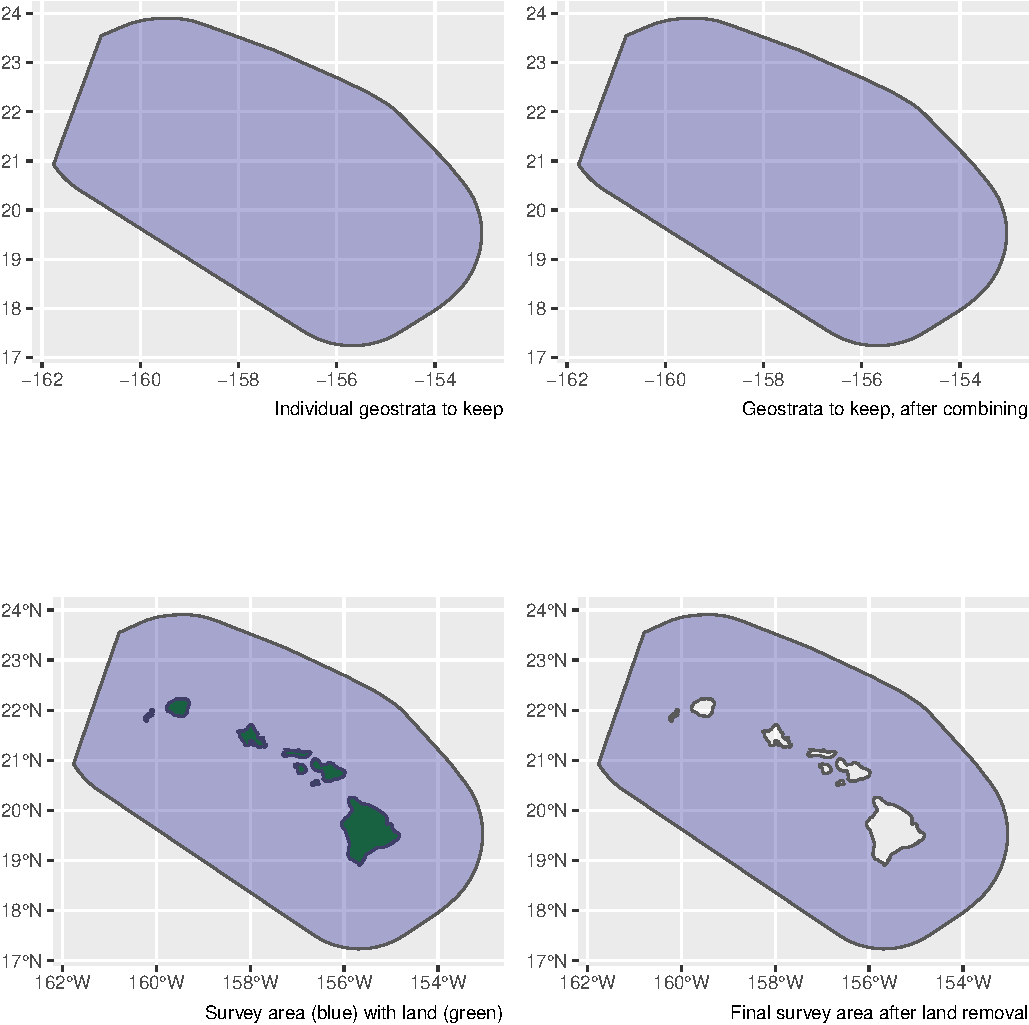
\includegraphics{figures/unnamed-chunk-190-1.pdf}

Say you want to estimate abundance in the pelagic Hawaiian EEZ, ignoring effort and sightings within the Main Hawaiian Islands stratum and accurately removing small islands in northwest Hawaii:

\begin{Shaded}
\begin{Highlighting}[]
\NormalTok{demo <-}\StringTok{ }\KeywordTok{strata_area}\NormalTok{(}\DataTypeTok{strata_all =}\NormalTok{ cruz}\OperatorTok{$}\NormalTok{settings}\OperatorTok{$}\NormalTok{strata,}
                    \DataTypeTok{strata_keep =} \KeywordTok{c}\NormalTok{(}\StringTok{'HI_EEZ'}\NormalTok{),}
                    \DataTypeTok{strata_remove =} \KeywordTok{c}\NormalTok{(}\StringTok{'MHI'}\NormalTok{),}
                    \DataTypeTok{verbose =} \OtherTok{FALSE}\NormalTok{)}
\end{Highlighting}
\end{Shaded}

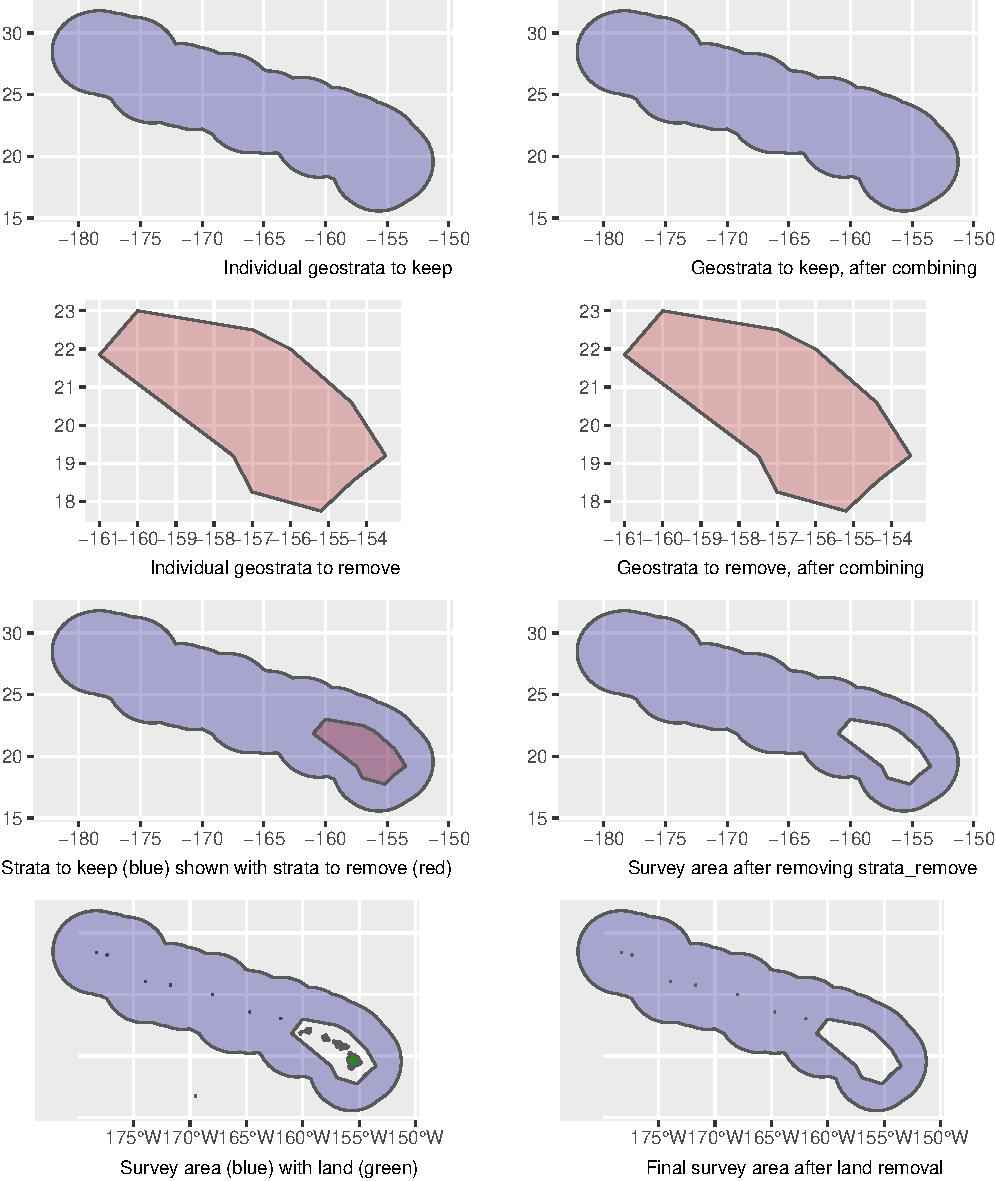
\includegraphics{figures/unnamed-chunk-191-1.pdf}

Say you want to estimate abundance of pelagic bottlenose dolphins within the WHICEAS study area, ignoring the insular stocks:

\begin{Shaded}
\begin{Highlighting}[]
\NormalTok{demo <-}\StringTok{ }\KeywordTok{strata_area}\NormalTok{(}\DataTypeTok{strata_all =}\NormalTok{ cruz}\OperatorTok{$}\NormalTok{settings}\OperatorTok{$}\NormalTok{strata,}
                    \DataTypeTok{strata_keep =} \KeywordTok{c}\NormalTok{(}\StringTok{'WHICEAS'}\NormalTok{),}
                    \DataTypeTok{strata_remove =} \KeywordTok{c}\NormalTok{(}\StringTok{'Bottlenose_KaNi'}\NormalTok{,}\StringTok{'Bottlenose_OUFI'}\NormalTok{,}\StringTok{'Bottlenose_BI'}\NormalTok{),}
                    \DataTypeTok{verbose =} \OtherTok{FALSE}\NormalTok{)}
\end{Highlighting}
\end{Shaded}

\includegraphics{figures/unnamed-chunk-192-1.pdf}

Say you want to estimate abundance for \emph{only} the insular bottlenose stocks:

\begin{Shaded}
\begin{Highlighting}[]
\NormalTok{demo <-}\StringTok{ }\KeywordTok{strata_area}\NormalTok{(}\DataTypeTok{strata_all =}\NormalTok{ cruz}\OperatorTok{$}\NormalTok{settings}\OperatorTok{$}\NormalTok{strata,}
                    \DataTypeTok{strata_keep =} \KeywordTok{c}\NormalTok{(}\StringTok{'Bottlenose_KaNi'}\NormalTok{,}\StringTok{'Bottlenose_OUFI'}\NormalTok{,}\StringTok{'Bottlenose_BI'}\NormalTok{),}
                    \DataTypeTok{verbose =} \OtherTok{FALSE}\NormalTok{)}
\end{Highlighting}
\end{Shaded}

\includegraphics{figures/unnamed-chunk-193-1.pdf}

Say you want to estimate abundance for false killer whales within the Northwest Hawaiian Islands and Main Hawaiian Islands study areas combined, but those geostrata partially overlap:

\begin{Shaded}
\begin{Highlighting}[]
\NormalTok{demo <-}\StringTok{ }\KeywordTok{strata_area}\NormalTok{(}\DataTypeTok{strata_all =}\NormalTok{ cruz}\OperatorTok{$}\NormalTok{settings}\OperatorTok{$}\NormalTok{strata,}
                    \DataTypeTok{strata_keep =} \KeywordTok{c}\NormalTok{(}\StringTok{'MHI'}\NormalTok{,}\StringTok{'NWHI'}\NormalTok{),}
                    \DataTypeTok{verbose =} \OtherTok{FALSE}\NormalTok{)}
\end{Highlighting}
\end{Shaded}

\includegraphics{figures/unnamed-chunk-194-1.pdf}

Say you want to estimate abundance for the Hawaiian EEZ \emph{outside} of those partially overlapping geostrata:

\begin{Shaded}
\begin{Highlighting}[]
\NormalTok{demo <-}\StringTok{ }\KeywordTok{strata_area}\NormalTok{(}\DataTypeTok{strata_all =}\NormalTok{ cruz}\OperatorTok{$}\NormalTok{settings}\OperatorTok{$}\NormalTok{strata,}
                    \DataTypeTok{strata_keep =} \StringTok{'HI_EEZ'}\NormalTok{,}
                    \DataTypeTok{strata_remove =} \KeywordTok{c}\NormalTok{(}\StringTok{'MHI'}\NormalTok{,}\StringTok{'NWHI'}\NormalTok{),}
                    \DataTypeTok{verbose =} \OtherTok{FALSE}\NormalTok{)}
\end{Highlighting}
\end{Shaded}

\includegraphics{figures/unnamed-chunk-195-1.pdf}

\hypertarget{g0-estimation}{%
\subsection*{\texorpdfstring{\emph{g(0)} estimation}{g(0) estimation}}\label{g0-estimation}}
\addcontentsline{toc}{subsection}{\emph{g(0)} estimation}

If you want \texttt{lta()} to calculate a weighted \emph{g(0)} estimate (and associated CV) that is specific to the conditions associated with your \texttt{estimates} sub-list parameters, all you need to do is provide the \texttt{Rg0} input. When you do this, the \texttt{lta()} function will find the \texttt{Rg0} values associated with the species code(s) in your \texttt{estimates} sub-list, then calculate weighted \emph{g(0)} and its CV using the \texttt{LTabundR} function, \texttt{g0\_weighted()}, which we discussed and demonstrated on the previous page.

If \texttt{lta()} can't find your species code in the \texttt{Rg0} table you provide, it will give up and assume that \texttt{g(0)} is 1.0 and that \texttt{g0\_cv} is 0.0.

If your \texttt{estimates} sub-list has a \texttt{alt\_g0\_spp} slot, \texttt{lta()} will use that species code instead to filter the \texttt{Rg0} table.

If your \texttt{estimates} sub-list has a \texttt{combine\_g0} slot that is \texttt{TRUE}, \texttt{lta()} will filter the \texttt{Rg0} table using all species codes you provide. If that filtration results in multiple \texttt{Rg0} species being found, weighted \emph{g(0)} will be calculated for each of those species separately, then those \emph{g(0)} estimates will be combined using a geometric mean (using the \texttt{LTabundR} function \texttt{g0\_combine()}). If \texttt{combine\_g0} is \texttt{FALSE}, only the first species code provided in your \texttt{estimates} sub-list will be used to filter \texttt{Rg0}.

If you want to supply a weighted \emph{g(0)} estimate and its CV yourself, you can add the \texttt{g0} and \texttt{g0\_cv} slots to your \texttt{estlimates} sublist, as explained above.

If you want to coerce \emph{g(0)} to be assumed to be 1.0 (with CV = 0.0), you can either (1) \emph{not} supply the \texttt{Rg0} input, or (2) manually specify the \texttt{g0} and \texttt{g0\_cv} slots in your \texttt{estimates} sub-list accordingly.

\hypertarget{covariates-in-detection-function-estimation}{%
\subsection*{Covariates in detection function estimation}\label{covariates-in-detection-function-estimation}}
\addcontentsline{toc}{subsection}{Covariates in detection function estimation}

Before detection functions are modelled, any covariates supplied by the user and specified as a factor are first tested for eligibility. Only factors with at least two levels (or whatever you specified with \texttt{df\_settings\$covariates\_levels}) and 10 observations in each level (or whatever you specified with \texttt{df\_settings\$covariates\_n\_per\_level}) are eligible for inclusion.

\hypertarget{fitting-a-detection-function}{%
\subsection*{Fitting a detection function}\label{fitting-a-detection-function}}
\addcontentsline{toc}{subsection}{Fitting a detection function}

The detection function is estimated using functions in the package \texttt{mrds}, primarily the main function \texttt{mrds::ddf()}, which uses a Horvitz-Thompson-like estimator to predict the probability of detection for each sighting. If multiple base key functions (e.g., half-normal or hazard-rate) are provided, and/or if covariates are specified, model fitting is done in a forward stepwise procedure:

\begin{itemize}
\tightlist
\item
  In the first round, the base model (no covariates, i.e., \texttt{"\textasciitilde{}1"}) is fit first.\\
\item
  In the second round, each covariate is added one at a time; at the end of the round, the covariate, if any, that produces the lowest AIC below the AIC from the previous round is added to the formula.\\
\item
  This process is repeated in subsequent rounds, adding a new covariate term in each round, until the AIC no longer improves.
\item
  If a second base key is provided, the process is repeated for that second key.
\end{itemize}

All models within \texttt{delta\_aic} of the model with the lowest AIC qualify as best-fitting models. The best-fitting model(s) is(are) then used to estimate the Effective Strip half-Width (ESW) based on the covariates associated with each sighting.

If multiple best-fitting models occur, we will find the average ESW for each sighting across all models, using a weighted mean approach in which we weight according to model AIC. To turn off this model averaging step, set \texttt{delta\_aic} to \texttt{0} to avoid passing multiple models to the abundance estimation stage.

This stage of the \texttt{lta()} command is executed within a backend function, \texttt{LTabundR::fit\_df()}, which has its own documentation for your reference.

\hypertarget{estimating-density-abundance}{%
\subsection*{Estimating density \& abundance}\label{estimating-density-abundance}}
\addcontentsline{toc}{subsection}{Estimating density \& abundance}

Estimates are produced for various combinations of species, regions, and years, according to the arguments specified in your \texttt{estimates} list(s). Before these estimates are produced, we filter the data used to fit the detection function to strictly systematic (design-based) effort (i.e., \texttt{EffType\ =\ "S"}), in which standard protocols are in use (i.e., \texttt{OnEffort\ =\ TRUE}) and the Beaufort sea state is less than 7 (though these controls can be modified using the \texttt{lta()} inputs \texttt{abund\_eff\_types} and \texttt{abund\_bft\_range} (see above).

This stage of the \texttt{lta()} command is executed within a back-end function, \texttt{LTabundR::abundance()}, which has its own documentation for your reference.

\hypertarget{bootstrap-variance-estimation}{%
\subsection*{Bootstrap variance estimation}\label{bootstrap-variance-estimation}}
\addcontentsline{toc}{subsection}{Bootstrap variance estimation}

If the \texttt{bootstraps} input value is greater than 1, bootstrap variance estimation will be attempted. In each bootstrap iteration, survey segments are re-sampled with replacement before fitting the detection function and estimating density/abundance. Re-sampling is done in a routine that preserves the proportion of segments from each geostratum.

Note that the entire process is repeated in each bootstrap: step-wise fitting of the detection function, averaging of the best-fitting models, and density/abundance estimation for all species/region/year combinations specified in your \texttt{estimates} input. At the end of the bootstrap process, results are summarized for each species/region/year combination. 95\% confidence intervals are calculated using the BCA method (package \texttt{coxed}, function \texttt{bca()}).

\hypertarget{g0-values-during-bootstrapping}{%
\subsection*{\texorpdfstring{\texttt{g(0)} values during bootstrapping}{g(0) values during bootstrapping}}\label{g0-values-during-bootstrapping}}
\addcontentsline{toc}{subsection}{\texttt{g(0)} values during bootstrapping}

When conducting the non-parametric bootstrap routine to estimate the CV of density and abundance, uncertainty is incorporated into the g(0) value in each iteration using a parametric bootstrapping subroutine: First, a logit-transformed distribution is modeled based upon the mean and CV of g(0) provided by the user in the \texttt{estimates} input (see documentation for \texttt{LTabundR::g0\_optimize()} for details on this step). This modeled distribution is used to randomly draw a g(0) value for each iteration of the density/abundance bootstrap routine. In this way, the uncertainty in g(0) is propagated into uncertainty in density/abundance.

\hypertarget{destratify}{%
\chapter{Stratified analysis}\label{destratify}}

Field surveys are sometimes stratified such that trackline design and/or density can differ substantially across regions. Also, analysts may sometimes wish to estimate density/abundance for individual regions separately, regardless of design stratification.

On the previous page, we demonstrated how to accommodate a stratified analysis by providing an \texttt{estimates} sub-list for each geostratum.

For example, in 2002 the Hawaiian EEZ was surveyed with different effort intensity in the Main Hawaiian Islands region compared to pelagic waters.

Here is the code that generates density/abundance estimates of striped dolphins in 2002 (stratified) and 2010 (unstratified), with only 10 bootstrap iterations:

\begin{Shaded}
\begin{Highlighting}[]
\CommentTok{# Survey data}
\KeywordTok{data}\NormalTok{(}\StringTok{"cnp_150km_1986_2020"}\NormalTok{)}
\NormalTok{cruz <-}\StringTok{ }\NormalTok{cnp_150km_}\DecValTok{1986}\NormalTok{_}\DecValTok{2020}

\CommentTok{# Rg0 table}
\KeywordTok{data}\NormalTok{(}\StringTok{"g0_results"}\NormalTok{)}
\NormalTok{Rg0 <-}\StringTok{ }\NormalTok{g0_results}

\CommentTok{# Detection function filters}
\NormalTok{fit_filters <-}\StringTok{ }\KeywordTok{list}\NormalTok{(}\DataTypeTok{spp =} \KeywordTok{c}\NormalTok{(}\StringTok{'013'}\NormalTok{, }\StringTok{'026'}\NormalTok{, }\StringTok{'031'}\NormalTok{), }
                   \DataTypeTok{pool =} \StringTok{'Multi-species pool 1'}\NormalTok{,}
                   \DataTypeTok{cohort =} \StringTok{'all'}\NormalTok{,}
                   \DataTypeTok{truncation_distance =} \DecValTok{5}\NormalTok{,}
                   \DataTypeTok{other_species =} \StringTok{'remove'}\NormalTok{)}

\CommentTok{# Detection function settings}
\NormalTok{df_settings <-}\StringTok{ }\KeywordTok{list}\NormalTok{(}\DataTypeTok{covariates =} \KeywordTok{c}\NormalTok{(}\StringTok{'bft'}\NormalTok{,}\StringTok{'lnsstot'}\NormalTok{,}\StringTok{'cruise'}\NormalTok{,}\StringTok{'year'}\NormalTok{,}\StringTok{'ship'}\NormalTok{,}\StringTok{'species'}\NormalTok{),}
                   \DataTypeTok{covariates_factor =} \KeywordTok{c}\NormalTok{(}\OtherTok{FALSE}\NormalTok{, }\OtherTok{FALSE}\NormalTok{, }\OtherTok{TRUE}\NormalTok{, }\OtherTok{TRUE}\NormalTok{, }\OtherTok{TRUE}\NormalTok{, }\OtherTok{TRUE}\NormalTok{),}
                   \DataTypeTok{covariates_levels =} \DecValTok{2}\NormalTok{,}
                   \DataTypeTok{covariates_n_per_level =} \DecValTok{10}\NormalTok{,}
                   \DataTypeTok{detection_function_base =} \StringTok{'hn'}\NormalTok{,}
                   \DataTypeTok{base_model =} \StringTok{'~1'}\NormalTok{,}
                   \DataTypeTok{delta_aic =} \DecValTok{2}\NormalTok{)}

\CommentTok{# Estimates}
\NormalTok{estimates <-}\StringTok{ }\KeywordTok{list}\NormalTok{(}
    \KeywordTok{list}\NormalTok{(}\DataTypeTok{spp =} \StringTok{'013'}\NormalTok{,}
         \DataTypeTok{title =} \StringTok{'Striped dolphin'}\NormalTok{,}
         \DataTypeTok{years =} \DecValTok{2002}\NormalTok{,}
         \DataTypeTok{regions =} \StringTok{'MHI'}\NormalTok{),}
    \KeywordTok{list}\NormalTok{(}\DataTypeTok{spp =} \StringTok{'013'}\NormalTok{,}
         \DataTypeTok{title =} \StringTok{'Striped dolphin'}\NormalTok{,}
         \DataTypeTok{years =} \DecValTok{2002}\NormalTok{,}
         \DataTypeTok{regions =} \StringTok{'HI_EEZ'}\NormalTok{,}
         \DataTypeTok{regions_remove =} \StringTok{'MHI'}\NormalTok{),}
    \KeywordTok{list}\NormalTok{(}\DataTypeTok{spp =} \StringTok{'013'}\NormalTok{,}
         \DataTypeTok{title =} \StringTok{'Striped dolphin'}\NormalTok{,}
         \DataTypeTok{years =} \DecValTok{2010}\NormalTok{,}
         \DataTypeTok{regions =} \StringTok{'HI_EEZ'}\NormalTok{))}

\CommentTok{# Run it}
\NormalTok{results <-}\StringTok{ }\KeywordTok{lta}\NormalTok{(cruz, Rg0, }
\NormalTok{               fit_filters, df_settings, estimates, }
               \DataTypeTok{bootstraps =} \DecValTok{10}\NormalTok{)}

\CommentTok{# Save it locally}
\KeywordTok{saveRDS}\NormalTok{(results, }\DataTypeTok{file=}\StringTok{'lta/multispecies_pool_1.RData'}\NormalTok{)}
\end{Highlighting}
\end{Shaded}

Let's read these results back in using the \texttt{LTabundR} function \texttt{lta\_enlist()}, which stores LTA results in a flexible list structure.

\begin{Shaded}
\begin{Highlighting}[]
\NormalTok{ltas <-}\StringTok{ }\KeywordTok{lta_enlist}\NormalTok{(}\StringTok{'lta/'}\NormalTok{)}
\end{Highlighting}
\end{Shaded}

As these results stand, 2002 estimates are stratified into 2 separate regions:

\begin{Shaded}
\begin{Highlighting}[]
\NormalTok{(ltas }\OperatorTok\StringTok{ }\KeywordTok{lta_report}\NormalTok{(}\DataTypeTok{verbose =} \OtherTok{FALSE}\NormalTok{))}\OperatorTok{$}\NormalTok{table4}
                         \DecValTok{2002}\NormalTok{ (HI_EEZ) }\OperatorTok{-}\StringTok{ }\NormalTok{(MHI)                       }\DecValTok{2002}
\DecValTok{1}\NormalTok{ Species or category Density        Abundance   CV        }\DecValTok{95}\NormalTok{% CI Density}
\DecValTok{2}\NormalTok{     Striped dolphin    }\FloatTok{14.2}           \DecValTok{32}\NormalTok{,}\DecValTok{135} \FloatTok{0.47} \DecValTok{16}\NormalTok{,}\DecValTok{707-64}\NormalTok{,}\DecValTok{184}   \FloatTok{12.06}
\NormalTok{      (MHI)                 }\DecValTok{2010}\NormalTok{  (HI_EEZ)                    }
\DecValTok{1}\NormalTok{ Abundance   CV  }\DecValTok{95}\OperatorTok\StringTok{ }\NormalTok{CI}
\DecValTok{2}     \DecValTok{2}\NormalTok{,}\DecValTok{557} \FloatTok{0.89} \DecValTok{0-7}\NormalTok{,}\DecValTok{491}   \FloatTok{23.86}    \DecValTok{59}\NormalTok{,}\DecValTok{051} \FloatTok{0.42} \DecValTok{45}\NormalTok{,}\DecValTok{459-131}\NormalTok{,}\DecValTok{350}
\end{Highlighting}
\end{Shaded}

Now let's process these LTA results through an \texttt{LTabundR} function, \texttt{lta\_destratify()}, which will combine the separate regional estimates from 2002 into a single estimate for the year.

\begin{Shaded}
\begin{Highlighting}[]
\NormalTok{ltas_2a <-}
\StringTok{  }\KeywordTok{lta_destratify}\NormalTok{(ltas,}
               \DataTypeTok{years =} \DecValTok{2002}\NormalTok{,}
               \DataTypeTok{combine_method =} \StringTok{'arithmetic'}\NormalTok{,}
               \DataTypeTok{new_region =} \StringTok{'(HI_EEZ)'}\NormalTok{)}
\end{Highlighting}
\end{Shaded}

The \texttt{new\_region} argument specifies how to refer to the combined region. In this case we want the 2002 study area to be named the same as the unstratified 2010 study area, hence \texttt{"(HI\_EEZ)"}. The \texttt{combine\_method} argument is explained below.

Now let's re-check the summary table:

\begin{Shaded}
\begin{Highlighting}[]
\NormalTok{(ltas_2a }\OperatorTok\StringTok{ }\KeywordTok{lta_report}\NormalTok{(}\DataTypeTok{verbose=}\OtherTok{FALSE}\NormalTok{))}\OperatorTok{$}\NormalTok{table4}
                         \DecValTok{2002}\NormalTok{  (HI_EEZ)                       }\DecValTok{2010}\NormalTok{  (HI_EEZ)}
\DecValTok{1}\NormalTok{ Species or category Density Abundance   CV        }\DecValTok{95}\NormalTok{% CI Density Abundance}
\DecValTok{2}\NormalTok{     Striped dolphin   }\FloatTok{14.02}    \DecValTok{34}\NormalTok{,}\DecValTok{691} \FloatTok{0.82} \DecValTok{8}\NormalTok{,}\DecValTok{462-142}\NormalTok{,}\DecValTok{221}   \FloatTok{23.86}    \DecValTok{59}\NormalTok{,}\DecValTok{051}
                     
\DecValTok{1}\NormalTok{   CV         }\DecValTok{95}\NormalTok{% CI}
\DecValTok{2} \FloatTok{0.42} \DecValTok{45}\NormalTok{,}\DecValTok{459-131}\NormalTok{,}\DecValTok{350}
\end{Highlighting}
\end{Shaded}

There is now only one set of columns for 2002, and the values therein are combinations of the stratified regions.

The ``de-stratification'' routine within \texttt{lta\_destratify()} sums abundance estimates across regions to get combined abundance. To estimate density in the combined regions, the function uses weighted averaging in which the area of a geostratum serves as its weight. To estimate CV and confidence interval of the combined result, the function uses one of two \texttt{combine\_methods} (this is an argument in the function). The default method is \texttt{"arithmetic"}, which uses classic formulae to estimate the combined variance and the corresponding confidence interval. This is done in a way that allows multiple geostrata to be combined, not just two.

The second option, \texttt{"bootstrap"}, uses an iterative method that draws bootstrap samples, with replacement, from the bootstrap estimate of density within each stratified region.

\begin{Shaded}
\begin{Highlighting}[]
\NormalTok{ltas_2b <-}
\StringTok{  }\KeywordTok{lta_destratify}\NormalTok{(ltas,}
               \DataTypeTok{years =} \DecValTok{2002}\NormalTok{,}
               \DataTypeTok{combine_method =} \StringTok{'bootstrap'}\NormalTok{,}
               \DataTypeTok{new_region =} \StringTok{'(HI_EEZ)'}\NormalTok{)}
\end{Highlighting}
\end{Shaded}

\begin{Shaded}
\begin{Highlighting}[]
\NormalTok{(ltas_2b }\OperatorTok\StringTok{ }\KeywordTok{lta_report}\NormalTok{(}\DataTypeTok{verbose=}\OtherTok{FALSE}\NormalTok{))}\OperatorTok{$}\NormalTok{table4}
                         \DecValTok{2002}\NormalTok{  (HI_EEZ)                      }\DecValTok{2010}\NormalTok{  (HI_EEZ)}
\DecValTok{1}\NormalTok{ Species or category Density Abundance  CV        }\DecValTok{95}\NormalTok{% CI Density Abundance}
\DecValTok{2}\NormalTok{     Striped dolphin   }\FloatTok{14.02}    \DecValTok{34}\NormalTok{,}\DecValTok{691} \FloatTok{0.4} \DecValTok{18}\NormalTok{,}\DecValTok{628-80}\NormalTok{,}\DecValTok{649}   \FloatTok{23.86}    \DecValTok{59}\NormalTok{,}\DecValTok{051}
                     
\DecValTok{1}\NormalTok{   CV         }\DecValTok{95}\NormalTok{% CI}
\DecValTok{2} \FloatTok{0.42} \DecValTok{45}\NormalTok{,}\DecValTok{459-131}\NormalTok{,}\DecValTok{350}
\end{Highlighting}
\end{Shaded}

Note that use of \texttt{lta\_destratify()} only makes sense if the stratified regions have zero overlap.

\hypertarget{trend-analysis}{%
\chapter{Trend analysis}\label{trend-analysis}}

When a species' density appears to change dramatically from one survey year to the next, it could be due to several factors: the species' abundance may have changed; its range may have shifted; or the timing of its migratory movements may have shifted. This apparent change could also be due solely to random chance: you can sample the exact same population in two different surveys, and you are liable to produce different abundance estimates due simply to random variation in how often you encounter your target species. In other words, \emph{random variation in the encounter rate} may lead you to estimate a change in abundance, when in fact there is no change.

For this reason, whenever you suspect that abundance has changed between years -- i.e., whenever the confidence intervals for two years do not overlap -- it is good practice to carry out follow-up tests. One such test was developed in (\href{https://www.fisheries.noaa.gov/inport/item/59592}{Bradford et al.~2020} and Bradford et al.~(2021). That test has been provided in \texttt{LTabundR} with the function \texttt{er\_simulator()}, which refers to a simulation-based test of random variation in the \textbf{e}ncounter \textbf{r}ate (ER).

This function uses randomization simulations to test for the probability that year-to-year changes observed in a species' encounter rate are due to random sampling variation (and not actual change in the encounter rate). More specifcially, this function uses bootstrap sampling of survey segments to see if random variation in sampling could possibly produce an apparent but immaterial change in encounter rate across years.

You will find full analytical details in the Appendix to Bradford et al.~(2020) for analytical details, but briefly: in each bootstrap iteration, survey segments are resampled in a way that preserves the proportion of effort occurring within each geostratum in the data. The resampled data are used to calculate the overall ER across all survey years, since the null hypothesis is that the ER does not change across years. This overall ER is used to predict the number of sightings in each year, based on the distance covered by the resampled segments in each year. This process is repeated (typically hundreds to thousands of times) to produce a distribution of predicted sighting counts in each year. This distribution reflects the range of ERs that could be possible due simply to random variation and \emph{not} to underlying changes in abundance. These distributions are compared to the actual number of sightings observed in their respective year. The fraction of simulated sightings counts that are more extreme than the observed count reflects the probability that the observed count is due to random sample variation alone.

For example, Bradford et al.~(2021) found non-overlapping confidence intervals in their estimates of Bryde's whale abundance in 2002, 2010, and 2017. To test for the significance of these trends, they carried out the ``ER simulator'' routine described above. In \texttt{LTabundR}, we would carry out the same analysis as follows:

Take your processed data:

\begin{Shaded}
\begin{Highlighting}[]
\KeywordTok{data}\NormalTok{(cnp_150km_}\DecValTok{1986}\NormalTok{_}\DecValTok{2020}\NormalTok{)}
\NormalTok{cruz <-}\StringTok{ }\NormalTok{cnp_150km_}\DecValTok{1986}\NormalTok{_}\DecValTok{2020}
\end{Highlighting}
\end{Shaded}

Filter it to systematic effort in the years of interest:

\begin{Shaded}
\begin{Highlighting}[]
\NormalTok{cruzi <-}\StringTok{ }
\StringTok{  }\KeywordTok{filter_cruz}\NormalTok{(cruz,}
              \DataTypeTok{analysis_only =} \OtherTok{TRUE}\NormalTok{,}
              \DataTypeTok{years =} \KeywordTok{c}\NormalTok{(}\DecValTok{2002}\NormalTok{, }\DecValTok{2010}\NormalTok{, }\DecValTok{2017}\NormalTok{),}
              \DataTypeTok{regions =} \StringTok{'HI_EEZ'}\NormalTok{,}
              \DataTypeTok{eff_types =} \StringTok{'S'}\NormalTok{,}
              \DataTypeTok{bft_range =} \DecValTok{0}\OperatorTok{:}\DecValTok{6}\NormalTok{)}
\end{Highlighting}
\end{Shaded}

Conduct the ER simulation, passing the species code for the Bryde's whale (\texttt{"072"}). For the purposes of this example, we will only use 100 iterations.

\begin{Shaded}
\begin{Highlighting}[]
\NormalTok{er_results <-}\StringTok{ }
\StringTok{  }\KeywordTok{er_simulator}\NormalTok{(}\DataTypeTok{spp =} \StringTok{'072'}\NormalTok{, }\DataTypeTok{cruz =}\NormalTok{ cruzi, }\DataTypeTok{iterations =} \DecValTok{100}\NormalTok{)}
\end{Highlighting}
\end{Shaded}

This routine provides a list with two slots:

\begin{Shaded}
\begin{Highlighting}[]
\NormalTok{er_results }\OperatorTok\StringTok{ }\NormalTok{names}
\NormalTok{[}\DecValTok{1}\NormalTok{] }\StringTok{"summary"} \StringTok{"details"}
\end{Highlighting}
\end{Shaded}

The \texttt{summary} slot returns the p-value for each year, i.e., the chances that the observed number of sightings was due purely to random variation in the encounter rate.

\begin{Shaded}
\begin{Highlighting}[]
\NormalTok{er_results}\OperatorTok{$}\NormalTok{summary}
\NormalTok{  years observed   p}
\DecValTok{1}  \DecValTok{2002}      \DecValTok{171} \FloatTok{1.0}
\DecValTok{2}  \DecValTok{2010}      \DecValTok{310} \FloatTok{0.0}
\DecValTok{3}  \DecValTok{2017}      \DecValTok{241} \FloatTok{0.8}
\end{Highlighting}
\end{Shaded}

In this example, the encounter rates observed in 2002 and 2010 are very likely due to some process \emph{other} than random variation in the encounter rate, such as range shifts, seasonal movement timing shifts, and/or changes in abundance. However, the observed encounter rate in 2017 could easily be explained by random variation in the ER.

The \texttt{details} slot returns the simulation predictions for each year, which can be used to replicate the histograms that are printed when the function is run.

\includegraphics{figures/unnamed-chunk-212-1.pdf}

A dataframe with a row for each year. Columns provide the number of observations of the species of interest during systematic effort, and the p-value of the test. The p-value represents the fraction of simulated encounter rates that exceed the observed encounter rate.

\hypertarget{subgroup-based-analysis}{%
\chapter{Subgroup-based analysis}\label{subgroup-based-analysis}}

False killer whales (\emph{Pseudorca crassidens}) are rare and occur in dispersed subgroups, which complicates conventional distance sampling approaches to line-transect analysis. To better estimate their abundance, in 2010 the Pacific Islands Fisheries Science Center (PIFSC) initiated a sub-group protocol referred to as the ``PC Protocol'', a reference to the species' scientific name.

To conduct line-transect analysis with this sub-group-based protocol, a method was developed in 2014 - 2017
To handle this, a separate, \emph{subgroup-based} analytical approach was developed in 2014 - 2017, then updated in 2020 (\href{https://www.fisheries.noaa.gov/inport/item/59592}{Bradford et al.~2020}).

An additional complication is that false killer whales in Hawaiian waters belong to two discrete populations -- the Northwest Hawaiian Islands (NWHI) population and a pelagic population -- whose ranges partially overlap, which means that population assignment cannot always be based simply on the geographic location of sightings. When geographic inference of population is not possible, biopsy-sampled genetics, photo-identification, and acoustics are used to assign each sighting to a population \emph{post-hoc}.

To accommodate these special circumstances with an appropriate balance of flexibility and efficiency, \texttt{LTabundR} includes a function named \texttt{lta\_subgroup()}, whose use will look something like this:

\begin{Shaded}
\begin{Highlighting}[]
\KeywordTok{lta_subgroup}\NormalTok{(df_sits,}
\NormalTok{             truncation_distance,}
\NormalTok{             ss,}
\NormalTok{             cruz10,}
\NormalTok{             g0_spp,}
\NormalTok{             g0_truncation,}
\NormalTok{             g0_pool_bft,}
             \DataTypeTok{g0_jackknife_fraction =} \FloatTok{0.1}\NormalTok{,}
\NormalTok{             density_segments,}
\NormalTok{             density_das,}
\NormalTok{             density_sightings,}
\NormalTok{             abundance_area,}
             \DataTypeTok{iterations =} \DecValTok{1000}\NormalTok{,}
             \DataTypeTok{output_dir =} \StringTok{'../test_code/subgroup/'}\NormalTok{,}
             \DataTypeTok{toplot =} \OtherTok{TRUE}\NormalTok{,}
             \DataTypeTok{verbose =} \OtherTok{TRUE}\NormalTok{,}
             \DataTypeTok{density_bootstraps =} \DecValTok{10000}\NormalTok{)}
\end{Highlighting}
\end{Shaded}

We will step through each of these inputs below, using a case study in which we estimate false killer whale abundance in the Hawaiian EEZ for 2017.

\hypertarget{inputs-1}{%
\section*{Inputs}\label{inputs-1}}
\addcontentsline{toc}{section}{Inputs}

\hypertarget{df_sits}{%
\subsection*{\texorpdfstring{\texttt{df\_sits}}{df\_sits}}\label{df_sits}}
\addcontentsline{toc}{subsection}{\texttt{df\_sits}}

This is a \texttt{data.frame} of sightings you want to use to fit the detection function model. For false killer whales in Bradford et al.~(2020), this is a combination of systematic sightings prior to 2010 and Phase 1 sightings from 2010 onwards (using the PC protocol). No filtering will be applied to these sightings within this function, so make sure you provide the data pre-filtered. Bradford et al.~(2020) used a single detection function for all populations of false killer whale.

\texttt{LTabundR} has a built-in dataset for processed Central North Pacific surveys, 1986-2020, using 150-km segments. We will use that here:

\begin{Shaded}
\begin{Highlighting}[]
\KeywordTok{data}\NormalTok{(}\StringTok{"cnp_150km_1986_2020"}\NormalTok{)}
\NormalTok{cruz <-}\StringTok{ }\NormalTok{cnp_150km_}\DecValTok{1986}\NormalTok{_}\DecValTok{2020}
\end{Highlighting}
\end{Shaded}

The code used to generate this dataset can be seen by pulling up the help documentation: \texttt{?noaa\_10km\_1986\_2020}.

As mentioned above, for 1986 - 2010, all detections are assumed to be `Phase 1' sightings, and therefore usable in detection function estimation. Here we draw those sightings from the above \texttt{cruz} object, filtering as needed (the species code for false killer whales is \texttt{"033"}), and to simplify we will select only a few key columns.

\begin{Shaded}
\begin{Highlighting}[]
\NormalTok{sits1  <-}
\StringTok{  }\NormalTok{cruz}\OperatorTok{$}\NormalTok{cohorts}\OperatorTok{$}\NormalTok{all}\OperatorTok{$}\NormalTok{sightings }\OperatorTok
\StringTok{  }\KeywordTok{filter}\NormalTok{(OnEffort }\OperatorTok{==}\StringTok{ }\OtherTok{TRUE}\NormalTok{,}
\NormalTok{         year }\OperatorTok{<}\StringTok{ }\DecValTok{2011}\NormalTok{,}
\NormalTok{         Lat }\OperatorTok{>=}\StringTok{ }\DecValTok{5}\NormalTok{, Lat }\OperatorTok{<=}\StringTok{ }\DecValTok{40}\NormalTok{, Lon }\OperatorTok{>=}\StringTok{ }\DecValTok{-185}\NormalTok{, Lon }\OperatorTok{<=}\StringTok{ }\DecValTok{-120}\NormalTok{,}
\NormalTok{         species }\OperatorTok{==}\StringTok{ '033'}\NormalTok{,}
\NormalTok{         mixed }\OperatorTok{==}\StringTok{ }\OtherTok{FALSE}\NormalTok{) }\OperatorTok
\StringTok{  }\KeywordTok{select}\NormalTok{(DateTime, Lat, Lon, Cruise, PerpDistKm)}

\NormalTok{sits1 }\OperatorTok\StringTok{ }\NormalTok{nrow}
\NormalTok{[}\DecValTok{1}\NormalTok{] }\DecValTok{33}

\NormalTok{sits1 }\OperatorTok\StringTok{ }\NormalTok{head}
\NormalTok{             DateTime       Lat       Lon Cruise PerpDistKm}
\DecValTok{1} \DecValTok{1986-11-13} \DecValTok{09}\OperatorTok{:}\DecValTok{43}\OperatorTok{:}\DecValTok{00} \FloatTok{10.466667} \FloatTok{-139.2833}    \DecValTok{990} \FloatTok{1.17493742}
\DecValTok{2} \DecValTok{1987-08-19} \DecValTok{15}\OperatorTok{:}\DecValTok{30}\OperatorTok{:}\DecValTok{00} \FloatTok{12.050000} \FloatTok{-133.3000}   \DecValTok{1080} \FloatTok{2.24543067}
\DecValTok{3} \DecValTok{1987-12-01} \DecValTok{09}\OperatorTok{:}\DecValTok{23}\OperatorTok{:}\DecValTok{00}  \FloatTok{8.266667} \FloatTok{-122.5500}   \DecValTok{1080} \FloatTok{0.42589077}
\DecValTok{4} \DecValTok{1989-08-22} \DecValTok{06}\OperatorTok{:}\DecValTok{45}\OperatorTok{:}\DecValTok{00} \FloatTok{11.800000} \FloatTok{-141.7333}   \DecValTok{1268} \FloatTok{0.40838431}
\DecValTok{5} \DecValTok{1989-08-22} \DecValTok{16}\OperatorTok{:}\DecValTok{39}\OperatorTok{:}\DecValTok{00} \FloatTok{12.716667} \FloatTok{-143.1000}   \DecValTok{1268} \FloatTok{0.68815211}
\DecValTok{6} \DecValTok{1989-09-10} \DecValTok{17}\OperatorTok{:}\DecValTok{18}\OperatorTok{:}\DecValTok{00}  \FloatTok{7.350000} \FloatTok{-129.5333}   \DecValTok{1268} \FloatTok{0.07751339}
\end{Highlighting}
\end{Shaded}

For 2011 onwards, we will use Phase 1 subgroup detections from the PC protocol, making sure that the column holding detection distances is named \texttt{PerpDistKm}:

\begin{Shaded}
\begin{Highlighting}[]
\NormalTok{sits2  <-}
\StringTok{  }\NormalTok{cruz}\OperatorTok{$}\NormalTok{cohorts}\OperatorTok{$}\NormalTok{all}\OperatorTok{$}\NormalTok{subgroups}\OperatorTok{$}\NormalTok{subgroups }\OperatorTok
\StringTok{  }\KeywordTok{filter}\NormalTok{(OnEffort }\OperatorTok{==}\StringTok{ }\OtherTok{TRUE}\NormalTok{,}
\NormalTok{         lubridate}\OperatorTok{::}\KeywordTok{year}\NormalTok{(DateTime) }\OperatorTok{>=}\StringTok{ }\DecValTok{2011}\NormalTok{,}
\NormalTok{         Lat }\OperatorTok{>=}\StringTok{ }\DecValTok{5}\NormalTok{, Lat }\OperatorTok{<=}\StringTok{ }\DecValTok{40}\NormalTok{, Lon }\OperatorTok{>=}\StringTok{ }\DecValTok{-185}\NormalTok{, Lon }\OperatorTok{<=}\StringTok{ }\DecValTok{-120}\NormalTok{,}
\NormalTok{         Species }\OperatorTok{==}\StringTok{ '033'}\NormalTok{,}
\NormalTok{         Phase }\OperatorTok{==}\StringTok{ }\DecValTok{1}\NormalTok{) }\OperatorTok
\StringTok{  }\KeywordTok{select}\NormalTok{(DateTime, Lat, Lon, Cruise, }\DataTypeTok{PerpDistKm =}\NormalTok{ PerpDist)}

\NormalTok{sits2 }\OperatorTok\StringTok{ }\NormalTok{nrow}
\NormalTok{[}\DecValTok{1}\NormalTok{] }\DecValTok{53}

\NormalTok{sits1 }\OperatorTok\StringTok{ }\NormalTok{head}
\NormalTok{             DateTime       Lat       Lon Cruise PerpDistKm}
\DecValTok{1} \DecValTok{1986-11-13} \DecValTok{09}\OperatorTok{:}\DecValTok{43}\OperatorTok{:}\DecValTok{00} \FloatTok{10.466667} \FloatTok{-139.2833}    \DecValTok{990} \FloatTok{1.17493742}
\DecValTok{2} \DecValTok{1987-08-19} \DecValTok{15}\OperatorTok{:}\DecValTok{30}\OperatorTok{:}\DecValTok{00} \FloatTok{12.050000} \FloatTok{-133.3000}   \DecValTok{1080} \FloatTok{2.24543067}
\DecValTok{3} \DecValTok{1987-12-01} \DecValTok{09}\OperatorTok{:}\DecValTok{23}\OperatorTok{:}\DecValTok{00}  \FloatTok{8.266667} \FloatTok{-122.5500}   \DecValTok{1080} \FloatTok{0.42589077}
\DecValTok{4} \DecValTok{1989-08-22} \DecValTok{06}\OperatorTok{:}\DecValTok{45}\OperatorTok{:}\DecValTok{00} \FloatTok{11.800000} \FloatTok{-141.7333}   \DecValTok{1268} \FloatTok{0.40838431}
\DecValTok{5} \DecValTok{1989-08-22} \DecValTok{16}\OperatorTok{:}\DecValTok{39}\OperatorTok{:}\DecValTok{00} \FloatTok{12.716667} \FloatTok{-143.1000}   \DecValTok{1268} \FloatTok{0.68815211}
\DecValTok{6} \DecValTok{1989-09-10} \DecValTok{17}\OperatorTok{:}\DecValTok{18}\OperatorTok{:}\DecValTok{00}  \FloatTok{7.350000} \FloatTok{-129.5333}   \DecValTok{1268} \FloatTok{0.07751339}
\end{Highlighting}
\end{Shaded}

To create \texttt{df\_sits} for detection function fitting, we combine these datasets together:

\begin{Shaded}
\begin{Highlighting}[]
\NormalTok{df_sits <-}\StringTok{ }\KeywordTok{rbind}\NormalTok{(sits1, sits2)}

\NormalTok{df_sits }\OperatorTok\StringTok{ }\NormalTok{nrow}
\NormalTok{[}\DecValTok{1}\NormalTok{] }\DecValTok{86}
\end{Highlighting}
\end{Shaded}

\hypertarget{truncation_distance}{%
\subsection*{\texorpdfstring{\texttt{truncation\_distance}}{truncation\_distance}}\label{truncation_distance}}
\addcontentsline{toc}{subsection}{\texttt{truncation\_distance}}

The truncation distance, in km, will be applied during detection function model fitting. Typically the farthest 5 - 10\% of sightings are truncated, but this needs to be balanced by sample size considerations.

Get candidate distances:

\begin{Shaded}
\begin{Highlighting}[]
\NormalTok{truncation_options <-}\StringTok{ }\KeywordTok{quantile}\NormalTok{(df_sits}\OperatorTok{$}\NormalTok{PerpDistKm, }
                               \KeywordTok{c}\NormalTok{(}\FloatTok{0.90}\NormalTok{,}\FloatTok{0.91}\NormalTok{,}\FloatTok{0.92}\NormalTok{,}\FloatTok{0.93}\NormalTok{,}\FloatTok{0.94}\NormalTok{,.}\DecValTok{95}\NormalTok{))}

\NormalTok{truncation_options}
     \DecValTok{90}\OperatorTok\StringTok{      }\DecValTok{92}\OperatorTok\StringTok{      }\DecValTok{94}\OperatorTok\StringTok{ }
\FloatTok{4.249637} \FloatTok{4.350266} \FloatTok{4.403387} \FloatTok{4.486396} \FloatTok{4.881672} \FloatTok{5.217843} 
\end{Highlighting}
\end{Shaded}

Plot these options:

\begin{Shaded}
\begin{Highlighting}[]
\KeywordTok{hist}\NormalTok{(df_sits}\OperatorTok{$}\NormalTok{PerpDistKm, }\DataTypeTok{main=}\StringTok{'Detection distances'}\NormalTok{)}
\KeywordTok{abline}\NormalTok{(}\DataTypeTok{v=}\NormalTok{truncation_options, }\DataTypeTok{col=}\StringTok{'red'}\NormalTok{, }\DataTypeTok{lty=}\DecValTok{3}\NormalTok{)}
\end{Highlighting}
\end{Shaded}

\includegraphics{figures/unnamed-chunk-220-1.pdf}

Get sample size remaining for each candidate distance:

\begin{Shaded}
\begin{Highlighting}[]
\KeywordTok{data.frame}\NormalTok{(}\DataTypeTok{km =}\NormalTok{ truncation_options, }
           \DataTypeTok{n =} \KeywordTok{sapply}\NormalTok{(truncation_options, }
                      \ControlFlowTok{function}\NormalTok{(x)\{}\KeywordTok{length}\NormalTok{(}\KeywordTok{which}\NormalTok{(df_sits}\OperatorTok{$}\NormalTok{PerpDistKm }\OperatorTok{<=}\StringTok{ }\NormalTok{x))\}))}
\NormalTok{          km  n}
\DecValTok{90}\NormalTok{% }\FloatTok{4.249637} \DecValTok{77}
\DecValTok{91}\NormalTok{% }\FloatTok{4.350266} \DecValTok{78}
\DecValTok{92}\NormalTok{% }\FloatTok{4.403387} \DecValTok{79}
\DecValTok{93}\NormalTok{% }\FloatTok{4.486396} \DecValTok{80}
\DecValTok{94}\NormalTok{% }\FloatTok{4.881672} \DecValTok{80}
\DecValTok{95}\NormalTok{% }\FloatTok{5.217843} \DecValTok{81}
\end{Highlighting}
\end{Shaded}

Based on these results, we will choose a truncation distance of 4.5 km.

\begin{Shaded}
\begin{Highlighting}[]
\NormalTok{truncation_distance <-}\StringTok{ }\FloatTok{4.5}
\end{Highlighting}
\end{Shaded}

\hypertarget{ss}{%
\subsection*{\texorpdfstring{\texttt{ss}}{ss}}\label{ss}}
\addcontentsline{toc}{subsection}{\texttt{ss}}

This is a numeric vector of subgroup school sizes. The function will find this vector's geometric mean and bootstrapped CV. In Bradford et al.~(2020), school size data come from all Phase 1 and Phase 2 estimates of subgroup sizes from 2010 onwards. In the processed \texttt{cruz} object, each of those estimates is the geometric mean of repeat estimates from separate observers.

\begin{Shaded}
\begin{Highlighting}[]
\NormalTok{ss  <-}
\StringTok{  }\NormalTok{cruz}\OperatorTok{$}\NormalTok{cohort}\OperatorTok{$}\NormalTok{all}\OperatorTok{$}\NormalTok{subgroups}\OperatorTok{$}\NormalTok{subgroups }\OperatorTok
\StringTok{  }\KeywordTok{filter}\NormalTok{(lubridate}\OperatorTok{::}\KeywordTok{year}\NormalTok{(DateTime) }\OperatorTok{>=}\StringTok{ }\DecValTok{2011}\NormalTok{,}
\NormalTok{         Lat }\OperatorTok{>=}\StringTok{ }\DecValTok{5}\NormalTok{, Lat }\OperatorTok{<=}\StringTok{ }\DecValTok{40}\NormalTok{, Lon }\OperatorTok{>=}\StringTok{ }\DecValTok{-185}\NormalTok{, Lon }\OperatorTok{<=}\StringTok{ }\DecValTok{-120}\NormalTok{,}
\NormalTok{         Species }\OperatorTok{==}\StringTok{ '033'}\NormalTok{) }\OperatorTok
\StringTok{  }\KeywordTok{pull}\NormalTok{(GSBest_geom)}
  
\NormalTok{ss }\OperatorTok\StringTok{ }\NormalTok{length}
\NormalTok{[}\DecValTok{1}\NormalTok{] }\DecValTok{183}

\NormalTok{ss}
\NormalTok{  [}\DecValTok{1}\NormalTok{]  }\FloatTok{5.00}  \FloatTok{7.00}  \FloatTok{1.00}  \FloatTok{1.00}  \FloatTok{1.00}  \FloatTok{1.33}  \FloatTok{2.00}  \FloatTok{2.75}  \FloatTok{2.67}  \FloatTok{1.00}  \FloatTok{6.00}  \FloatTok{1.00}
\NormalTok{ [}\DecValTok{13}\NormalTok{]  }\FloatTok{2.00} \FloatTok{18.50}  \FloatTok{1.00}  \FloatTok{4.00}  \FloatTok{5.00}  \FloatTok{2.00}  \FloatTok{1.00}  \FloatTok{4.00}  \FloatTok{4.50}  \FloatTok{2.50}  \FloatTok{2.00}  \FloatTok{2.00}
\NormalTok{ [}\DecValTok{25}\NormalTok{]  }\FloatTok{1.00}  \FloatTok{1.00}  \FloatTok{5.00}  \FloatTok{1.00}  \FloatTok{4.00}  \FloatTok{1.00}  \FloatTok{1.00}  \FloatTok{1.00}  \FloatTok{1.00}  \FloatTok{1.00}  \FloatTok{1.00}  \FloatTok{2.00}
\NormalTok{ [}\DecValTok{37}\NormalTok{]  }\FloatTok{2.00}  \FloatTok{1.00}  \FloatTok{4.00}  \FloatTok{9.83}  \FloatTok{2.50}  \FloatTok{4.75}  \FloatTok{8.25}  \FloatTok{3.00}  \FloatTok{2.00}  \FloatTok{3.00}  \FloatTok{3.67}  \FloatTok{3.50}
\NormalTok{ [}\DecValTok{49}\NormalTok{]  }\FloatTok{4.50}  \FloatTok{2.00}  \FloatTok{1.00}  \FloatTok{1.00}  \FloatTok{2.00}  \FloatTok{1.00}  \FloatTok{1.00}  \FloatTok{1.00}  \FloatTok{1.00}  \FloatTok{1.00}  \FloatTok{2.00}  \FloatTok{1.00}
\NormalTok{ [}\DecValTok{61}\NormalTok{]  }\FloatTok{1.00}  \FloatTok{1.00}  \FloatTok{2.00}  \FloatTok{3.00}  \FloatTok{2.00}  \FloatTok{1.50}  \FloatTok{2.67}  \FloatTok{1.33}  \FloatTok{2.00}  \FloatTok{6.00}  \FloatTok{4.33}  \FloatTok{2.00}
\NormalTok{ [}\DecValTok{73}\NormalTok{]  }\FloatTok{1.00}  \FloatTok{3.00}  \FloatTok{5.00}  \FloatTok{5.80}  \FloatTok{4.00}  \FloatTok{1.00}  \FloatTok{2.00}  \FloatTok{2.00}  \FloatTok{4.00}  \FloatTok{4.50}  \FloatTok{2.00}  \FloatTok{2.00}
\NormalTok{ [}\DecValTok{85}\NormalTok{]  }\FloatTok{2.00}  \FloatTok{4.50}  \FloatTok{2.00}  \FloatTok{1.00}  \FloatTok{2.00}  \FloatTok{1.00}  \FloatTok{1.00}  \FloatTok{2.00}  \FloatTok{2.00}  \FloatTok{1.50}  \FloatTok{4.50}  \FloatTok{1.00}
\NormalTok{ [}\DecValTok{97}\NormalTok{]  }\FloatTok{1.00}  \FloatTok{3.33}  \FloatTok{3.00}  \FloatTok{2.00}  \FloatTok{2.00}  \FloatTok{7.50}  \FloatTok{5.00}  \FloatTok{4.00}  \FloatTok{3.67}  \FloatTok{2.00}  \FloatTok{3.00}  \FloatTok{2.00}
\NormalTok{[}\DecValTok{109}\NormalTok{]  }\FloatTok{8.50}  \FloatTok{8.00}  \FloatTok{4.00}  \FloatTok{2.00}  \FloatTok{1.00}  \FloatTok{1.00}  \FloatTok{4.00}  \FloatTok{4.00}  \FloatTok{2.00}  \FloatTok{1.00}  \FloatTok{2.00}  \FloatTok{6.00}
\NormalTok{[}\DecValTok{121}\NormalTok{]  }\FloatTok{2.00}  \FloatTok{2.00}  \FloatTok{2.50}  \FloatTok{1.00}  \FloatTok{1.00}  \FloatTok{1.00}  \FloatTok{1.00}  \FloatTok{1.00}  \FloatTok{2.00}  \FloatTok{2.00}  \FloatTok{1.00}  \FloatTok{1.00}
\NormalTok{[}\DecValTok{133}\NormalTok{]  }\FloatTok{1.00}  \FloatTok{1.00}  \FloatTok{1.00}  \FloatTok{1.00}  \FloatTok{1.00}  \FloatTok{2.00}  \FloatTok{1.00}  \FloatTok{2.00}  \FloatTok{2.00}  \FloatTok{2.00}  \FloatTok{1.00}  \FloatTok{4.00}
\NormalTok{[}\DecValTok{145}\NormalTok{]  }\FloatTok{7.50}  \FloatTok{1.50}  \FloatTok{2.00}  \FloatTok{1.00}  \FloatTok{1.00}  \FloatTok{1.00}  \FloatTok{1.00}  \FloatTok{2.00}  \FloatTok{1.00}  \FloatTok{2.00}  \FloatTok{3.00}  \FloatTok{3.00}
\NormalTok{[}\DecValTok{157}\NormalTok{]  }\FloatTok{2.00}  \FloatTok{3.00}  \FloatTok{1.50}  \FloatTok{1.00}  \FloatTok{1.00}  \FloatTok{3.00}  \FloatTok{2.00}  \FloatTok{4.00}  \FloatTok{1.00}  \FloatTok{1.00}  \FloatTok{1.00}  \FloatTok{2.00}
\NormalTok{[}\DecValTok{169}\NormalTok{]  }\FloatTok{2.00}  \FloatTok{4.00}  \FloatTok{2.00}  \FloatTok{2.00}  \FloatTok{1.00}  \FloatTok{1.00}  \FloatTok{3.00}  \FloatTok{1.00}  \FloatTok{3.00}  \FloatTok{2.50}  \FloatTok{2.00}  \FloatTok{2.00}
\NormalTok{[}\DecValTok{181}\NormalTok{]  }\FloatTok{1.00}  \FloatTok{1.00}  \FloatTok{1.00}
\end{Highlighting}
\end{Shaded}

\hypertarget{cruz10}{%
\subsection*{\texorpdfstring{\texttt{cruz10}}{cruz10}}\label{cruz10}}
\addcontentsline{toc}{subsection}{\texttt{cruz10}}

This is a processed \texttt{cruz} object with short segment lengths, ideally 10 km or less (hence the 10 in the input name). This \texttt{cruz} object will be used to estimate \emph{Rg(0)}, i.e., the relative trackline detection probability (see its chapter). \texttt{LTabundR} comes with a built-in dataset we can use for this purpose:

\begin{Shaded}
\begin{Highlighting}[]
\KeywordTok{data}\NormalTok{(}\StringTok{"noaa_10km_1986_2020"}\NormalTok{)}
\NormalTok{cruz10 <-}\StringTok{ }\NormalTok{noaa_10km_}\DecValTok{1986}\NormalTok{_}\DecValTok{2020}
\end{Highlighting}
\end{Shaded}

The code used to generate this dataset can be seen by pulling up the help documentation: \texttt{?noaa\_10km\_1986\_2020}.

\hypertarget{g0_spp}{%
\subsection*{\texorpdfstring{\texttt{g0\_spp}}{g0\_spp}}\label{g0_spp}}
\addcontentsline{toc}{subsection}{\texttt{g0\_spp}}

This is a character vector of species code(s) to use to estimate \emph{Rg(0)}. In most cases this will be a single species, e.g., \texttt{"033"} for false killer whales.

\begin{Shaded}
\begin{Highlighting}[]
\NormalTok{g0_spp <-}\StringTok{ '033'}
\end{Highlighting}
\end{Shaded}

\hypertarget{g0_truncation}{%
\subsection*{\texorpdfstring{\texttt{g0\_truncation}}{g0\_truncation}}\label{g0_truncation}}
\addcontentsline{toc}{subsection}{\texttt{g0\_truncation}}

The truncation distance to use when estimating Rg(0). In Bradford et al.~(2020) this is 5.5 km.

\begin{Shaded}
\begin{Highlighting}[]
\NormalTok{g0_truncation <-}\StringTok{ }\FloatTok{5.5}
\end{Highlighting}
\end{Shaded}

\hypertarget{g0_pool_bft}{%
\subsection*{\texorpdfstring{\texttt{g0\_pool\_bft}}{g0\_pool\_bft}}\label{g0_pool_bft}}
\addcontentsline{toc}{subsection}{\texttt{g0\_pool\_bft}}

A way to specify that low Beaufort sea states, which are typically rare in open-ocean surveys, should be pooled. This step may be needed in order to achieve a monotonic decline in the \emph{g(0)} \textasciitilde{} Bft relationship, but the default is \texttt{NULL}, i.e., no pooling. If \texttt{g0\_pool\_bft} is the character string \texttt{"01"}, Beaufort states 1 will be pooled into state 0. If \texttt{g0\_pool\_bft} is the character string \texttt{"012"}, Beaufort states 1 and 2 will be pooled into state 0.

\begin{Shaded}
\begin{Highlighting}[]
\NormalTok{g0_pool_bft =}\StringTok{ }\OtherTok{NULL}
\end{Highlighting}
\end{Shaded}

\hypertarget{g0_jackknife_fraction}{%
\subsection*{\texorpdfstring{\texttt{g0\_jackknife\_fraction}}{g0\_jackknife\_fraction}}\label{g0_jackknife_fraction}}
\addcontentsline{toc}{subsection}{\texttt{g0\_jackknife\_fraction}}

The proportion of data to leave out within each jackknife permutation. The default is \texttt{0.1} (i.e., 10\% of the data, yielding 10 jackknife loops), after Barlow (2015).

\begin{Shaded}
\begin{Highlighting}[]
\NormalTok{g0_jackknife_fraction =}\StringTok{ }\FloatTok{0.1}
\end{Highlighting}
\end{Shaded}

\hypertarget{density_segments}{%
\subsection*{\texorpdfstring{\texttt{density\_segments}}{density\_segments}}\label{density_segments}}
\addcontentsline{toc}{subsection}{\texttt{density\_segments}}

The survey segments to be used in density/abundance estimation. For example, Bradford et al.~(2020) used 150-km segments to estimate false killer whale density in the Hawaiian EEZ in 2017. For this we can use the 1986-2020 dataset we loaded above. Note that no filtering will be applied to these segments by the \texttt{lta\_subgroup()} function, so w need to filter them ourselves first: we want only systematic segments for the Hawaiian EEZ in 2017 (specially, just cruises 1705 and 1706).

\begin{Shaded}
\begin{Highlighting}[]
\NormalTok{cruzi <-}\StringTok{ }\KeywordTok{filter_cruz}\NormalTok{(}\DataTypeTok{cruz =}\NormalTok{ cruz,}
                      \DataTypeTok{analysis_only =} \OtherTok{TRUE}\NormalTok{,}
                      \DataTypeTok{years =} \DecValTok{2017}\NormalTok{,}
                      \DataTypeTok{cruises =} \KeywordTok{c}\NormalTok{(}\DecValTok{1705}\NormalTok{, }\DecValTok{1706}\NormalTok{),}
                      \DataTypeTok{regions =} \StringTok{'HI_EEZ'}\NormalTok{,}
                      \DataTypeTok{bft_range =} \DecValTok{0}\OperatorTok{:}\DecValTok{6}\NormalTok{,}
                      \DataTypeTok{eff_types =} \StringTok{'S'}\NormalTok{,}
                      \DataTypeTok{on_off =} \OtherTok{TRUE}\NormalTok{)}
\end{Highlighting}
\end{Shaded}

From this filtered cruz object, we will isolate the segments data:

\begin{Shaded}
\begin{Highlighting}[]
\NormalTok{density_segments <-}\StringTok{ }\NormalTok{cruzi}\OperatorTok{$}\NormalTok{cohorts}\OperatorTok{$}\NormalTok{all}\OperatorTok{$}\NormalTok{segments}
\end{Highlighting}
\end{Shaded}

Since we do not want to stratify our analysis by smaller geostrata, such as the Main Hawaiian Islands, we will go ahead and coerce all stratum assignments to the Hawaiian EEZ geostratum:

\begin{Shaded}
\begin{Highlighting}[]
\NormalTok{density_segments}\OperatorTok{$}\NormalTok{stratum <-}\StringTok{ 'HI_EEZ'}
\end{Highlighting}
\end{Shaded}

\hypertarget{density_das}{%
\subsection*{\texorpdfstring{\texttt{density\_das}}{density\_das}}\label{density_das}}
\addcontentsline{toc}{subsection}{\texttt{density\_das}}

This is the complete survey data corresponding to the above segments. These data will be used to determine the proportion of survey effort occurring in each Beaufort sea state during estimation of \emph{Relative g(0)}.

\begin{Shaded}
\begin{Highlighting}[]
\NormalTok{density_das <-}\StringTok{ }\NormalTok{cruzi}\OperatorTok{$}\NormalTok{cohorts}\OperatorTok{$}\NormalTok{all}\OperatorTok{$}\NormalTok{das}
\end{Highlighting}
\end{Shaded}

\hypertarget{density_sightings}{%
\subsection*{\texorpdfstring{\texttt{density\_sightings}}{density\_sightings}}\label{density_sightings}}
\addcontentsline{toc}{subsection}{\texttt{density\_sightings}}

These are the encounters to use in density/abundance estimation. In Bradford et al.~(20120), these were the Phase 1 detections of false killer whale subgroups within the population-region-year of interest, e.g., Northwest Hawaiian Island population sightings within the Hawaiian EEZ in 2017. No filtering is applied to these sightings within \texttt{lta\_subgroups()}, so make sure only the sightings you wish to use are included and nothing more.

In this example, since we do not have population information on hand, we will not filter detections to a specific population. Instead, we will estimate abundance of all false killer whales within the Hawaiian EEZ:

\begin{Shaded}
\begin{Highlighting}[]
\NormalTok{density_sightings  <-}
\StringTok{  }\NormalTok{cruz}\OperatorTok{$}\NormalTok{cohorts}\OperatorTok{$}\NormalTok{all}\OperatorTok{$}\NormalTok{subgroups}\OperatorTok{$}\NormalTok{subgroups }\OperatorTok
\StringTok{  }\KeywordTok{filter}\NormalTok{(EffType }\OperatorTok{==}\StringTok{ 'S'}\NormalTok{,}
\NormalTok{         OnEffort }\OperatorTok{==}\StringTok{ }\OtherTok{TRUE}\NormalTok{,}
\NormalTok{         lubridate}\OperatorTok{::}\KeywordTok{year}\NormalTok{(DateTime) }\OperatorTok{==}\StringTok{ }\DecValTok{2017}\NormalTok{,}
\NormalTok{         PerpDist }\OperatorTok{<=}\StringTok{ }\NormalTok{truncation_distance,}
\NormalTok{         Species }\OperatorTok{==}\StringTok{ '033'}\NormalTok{,}
\NormalTok{         Phase }\OperatorTok{==}\StringTok{ }\DecValTok{1}\NormalTok{)}

\NormalTok{density_sightings }\OperatorTok\StringTok{ }\NormalTok{nrow}
\NormalTok{[}\DecValTok{1}\NormalTok{] }\DecValTok{32}

\NormalTok{density_sightings }\OperatorTok\StringTok{ }\NormalTok{head}
\NormalTok{  Cruise       Date            DateTime      Lat       Lon OnEffort Bft EffType}
\DecValTok{1}   \DecValTok{1705} \DecValTok{2017-09-21} \DecValTok{2017-09-21} \DecValTok{14}\OperatorTok{:}\DecValTok{17}\OperatorTok{:}\DecValTok{27} \FloatTok{20.04283} \FloatTok{-161.9177}     \OtherTok{TRUE}   \DecValTok{5}\NormalTok{       S}
\DecValTok{2}   \DecValTok{1705} \DecValTok{2017-09-21} \DecValTok{2017-09-21} \DecValTok{14}\OperatorTok{:}\DecValTok{39}\OperatorTok{:}\DecValTok{40} \FloatTok{20.06017} \FloatTok{-161.9840}     \OtherTok{TRUE}   \DecValTok{5}\NormalTok{       S}
\DecValTok{3}   \DecValTok{1705} \DecValTok{2017-09-29} \DecValTok{2017-09-29} \DecValTok{13}\OperatorTok{:}\DecValTok{22}\OperatorTok{:}\DecValTok{08} \FloatTok{23.55750} \FloatTok{-175.8527}     \OtherTok{TRUE}   \DecValTok{1}\NormalTok{       S}
\DecValTok{4}   \DecValTok{1705} \DecValTok{2017-09-29} \DecValTok{2017-09-29} \DecValTok{13}\OperatorTok{:}\DecValTok{26}\OperatorTok{:}\DecValTok{05} \FloatTok{23.56050} \FloatTok{-175.8643}     \OtherTok{TRUE}   \DecValTok{1}\NormalTok{       S}
\DecValTok{5}   \DecValTok{1705} \DecValTok{2017-09-29} \DecValTok{2017-09-29} \DecValTok{13}\OperatorTok{:}\DecValTok{26}\OperatorTok{:}\DecValTok{43} \FloatTok{23.56083} \FloatTok{-175.8662}     \OtherTok{TRUE}   \DecValTok{1}\NormalTok{       S}
\DecValTok{6}   \DecValTok{1705} \DecValTok{2017-09-29} \DecValTok{2017-09-29} \DecValTok{13}\OperatorTok{:}\DecValTok{32}\OperatorTok{:}\DecValTok{33} \FloatTok{23.56517} \FloatTok{-175.8832}     \OtherTok{TRUE}   \DecValTok{1}\NormalTok{       S}
\NormalTok{  SightNo Species SubGrp Angle   RadDist seg_id  PerpDist GSBest GSH  GSL}
\DecValTok{1}     \DecValTok{064}     \DecValTok{033}\NormalTok{      A    }\DecValTok{14} \FloatTok{5.0374102}   \DecValTok{1602} \FloatTok{1.2186598}   \FloatTok{3.00}   \DecValTok{4} \FloatTok{2.00}
\DecValTok{2}     \DecValTok{064}     \DecValTok{033}\NormalTok{      B    }\DecValTok{24} \FloatTok{3.1483814}   \DecValTok{1602} \FloatTok{1.2805621}   \FloatTok{3.67}   \DecValTok{6} \FloatTok{2.33}
\DecValTok{3}     \DecValTok{073}     \DecValTok{033}\NormalTok{      A    }\DecValTok{49} \FloatTok{3.3706200}   \DecValTok{1610} \FloatTok{2.5438392}   \FloatTok{2.00}   \DecValTok{3} \FloatTok{1.00}
\DecValTok{4}     \DecValTok{073}     \DecValTok{033}\NormalTok{      B    }\DecValTok{68} \FloatTok{0.6852359}   \DecValTok{1610} \FloatTok{0.6353397}   \FloatTok{1.00}   \DecValTok{2} \FloatTok{1.00}
\DecValTok{5}     \DecValTok{073}     \DecValTok{033}\NormalTok{      C    }\DecValTok{40} \FloatTok{0.3703978}   \DecValTok{1610} \FloatTok{0.2380871}   \FloatTok{1.00}   \DecValTok{1} \FloatTok{1.00}
\DecValTok{6}     \DecValTok{073}     \DecValTok{033}\NormalTok{      E    }\DecValTok{89} \FloatTok{2.9817023}   \DecValTok{1610} \FloatTok{2.9812482}   \FloatTok{1.00}   \DecValTok{2} \FloatTok{1.00}
\NormalTok{  GSBest_geom GSH_geom GSL_geom  use stratum_HI_EEZ stratum_OtherCNP}
\DecValTok{1}        \FloatTok{3.00}        \DecValTok{4}     \FloatTok{2.00} \OtherTok{TRUE}           \OtherTok{TRUE}             \OtherTok{TRUE}
\DecValTok{2}        \FloatTok{3.67}        \DecValTok{6}     \FloatTok{2.33} \OtherTok{TRUE}           \OtherTok{TRUE}             \OtherTok{TRUE}
\DecValTok{3}        \FloatTok{2.00}        \DecValTok{3}     \FloatTok{1.00} \OtherTok{TRUE}           \OtherTok{TRUE}             \OtherTok{TRUE}
\DecValTok{4}        \FloatTok{1.00}        \DecValTok{2}     \FloatTok{1.00} \OtherTok{TRUE}           \OtherTok{TRUE}             \OtherTok{TRUE}
\DecValTok{5}        \FloatTok{1.00}        \DecValTok{1}     \FloatTok{1.00} \OtherTok{TRUE}           \OtherTok{TRUE}             \OtherTok{TRUE}
\DecValTok{6}        \FloatTok{1.00}        \DecValTok{2}     \FloatTok{1.00} \OtherTok{TRUE}           \OtherTok{TRUE}             \OtherTok{TRUE}
\NormalTok{  stratum_MHI stratum Phase}
\DecValTok{1}       \OtherTok{FALSE}\NormalTok{  HI_EEZ     }\DecValTok{1}
\DecValTok{2}       \OtherTok{FALSE}\NormalTok{  HI_EEZ     }\DecValTok{1}
\DecValTok{3}       \OtherTok{FALSE}\NormalTok{  HI_EEZ     }\DecValTok{1}
\DecValTok{4}       \OtherTok{FALSE}\NormalTok{  HI_EEZ     }\DecValTok{1}
\DecValTok{5}       \OtherTok{FALSE}\NormalTok{  HI_EEZ     }\DecValTok{1}
\DecValTok{6}       \OtherTok{FALSE}\NormalTok{  HI_EEZ     }\DecValTok{1}
\end{Highlighting}
\end{Shaded}

As above, let's make sure the geostratum assignments for these sightings are simple:

\begin{Shaded}
\begin{Highlighting}[]
\NormalTok{density_segments}\OperatorTok{$}\NormalTok{stratum <-}\StringTok{ 'HI_EEZ'}
\end{Highlighting}
\end{Shaded}

\hypertarget{abundance_area}{%
\subsection*{\texorpdfstring{\texttt{abundance\_area}}{abundance\_area}}\label{abundance_area}}
\addcontentsline{toc}{subsection}{\texttt{abundance\_area}}

This is the area, in square km, of the region of interest. The density estimate will be scaled by this area.

We have two options for finding this area. The first is to draw the area from our \texttt{cohort\$strata} slot:

\begin{Shaded}
\begin{Highlighting}[]
\NormalTok{cruz}\OperatorTok{$}\NormalTok{strata}\OperatorTok{$}\NormalTok{area[cruz}\OperatorTok{$}\NormalTok{strata}\OperatorTok{$}\NormalTok{stratum }\OperatorTok{==}\StringTok{ 'HI_EEZ'}\NormalTok{]}
\NormalTok{[}\DecValTok{1}\NormalTok{] }\DecValTok{2474596}
\end{Highlighting}
\end{Shaded}

The second is to calculate it ourselves using the \texttt{LTabundR} function \texttt{strata\_area()}. This second option will be useful if your study area is a complicated combination/substraction of multiple geostrata.

\begin{Shaded}
\begin{Highlighting}[]
\KeywordTok{data}\NormalTok{(strata_cnp)}

\NormalTok{abundance_area <-}\StringTok{ }
\StringTok{  }\KeywordTok{strata_area}\NormalTok{(}\DataTypeTok{strata_all =}\NormalTok{ strata_cnp,}
              \DataTypeTok{strata_keep =} \StringTok{'HI_EEZ'}\NormalTok{)}\OperatorTok{$}\NormalTok{km2}
\end{Highlighting}
\end{Shaded}

\includegraphics{figures/unnamed-chunk-236-1.pdf}

\begin{Shaded}
\begin{Highlighting}[]

\NormalTok{abundance_area}
\NormalTok{[}\DecValTok{1}\NormalTok{] }\DecValTok{2474596}
\end{Highlighting}
\end{Shaded}

\hypertarget{remaining-inputs}{%
\subsection*{Remaining inputs}\label{remaining-inputs}}
\addcontentsline{toc}{subsection}{Remaining inputs}

\textbf{\texttt{iterations}}: Number of iterations to use in the various CV bootstrapping procedures occurring throughout this function, specifically: Effective Strip Half-Width CV estimation, school size CV estimation, weighted g(0) CV estimation, and encounter rate estimation.

\textbf{\texttt{output\_dir}}: The path in which results RData files should be stored. If left "", the current working directory will be used.

\textbf{\texttt{toplot}}: A Boolean, with default FALSE, indicating whether to plot various aspects of the analysis.

\textbf{\texttt{verbose}}: A Boolean, with default TRUE, indicating whether to print status updates to the Console.

\textbf{\texttt{density\_bootstraps}}: Number of bootstrap iterations to use for the CV estimate of density and abundance specifically. This input allows this final step to use a different (typically larger) iteration size than the iterations input above.

\begin{Shaded}
\begin{Highlighting}[]
\KeywordTok{save}\NormalTok{(results_subgroup, }\DataTypeTok{file=}\StringTok{'results_subgroup.RData'}\NormalTok{)}
\end{Highlighting}
\end{Shaded}

\begin{Shaded}
\begin{Highlighting}[]
\KeywordTok{load}\NormalTok{(}\StringTok{'results_subgroup.RData'}\NormalTok{)}
\end{Highlighting}
\end{Shaded}

\hypertarget{outputs-1}{%
\section*{Outputs}\label{outputs-1}}
\addcontentsline{toc}{section}{Outputs}

The function returns a \texttt{list} with many slots, including estimates of density and abundance -- along with estimates of intermediate parameters -- with a CV derived from a bootstrapping routine. To demonstrate this output, we will use results from a call with only 10 bootstrap iterations.

\begin{Shaded}
\begin{Highlighting}[]
\NormalTok{results_subgroup }\OperatorTok\StringTok{ }\NormalTok{names}
\NormalTok{ [}\DecValTok{1}\NormalTok{] }\StringTok{"D"}                  \StringTok{"D_CV"}               \StringTok{"D_L95"}             
\NormalTok{ [}\DecValTok{4}\NormalTok{] }\StringTok{"D_U95"}              \StringTok{"N"}                  \StringTok{"N_CV"}              
\NormalTok{ [}\DecValTok{7}\NormalTok{] }\StringTok{"N_L95"}              \StringTok{"N_U95"}              \StringTok{"ER"}                
\NormalTok{[}\DecValTok{10}\NormalTok{] }\StringTok{"ss"}                 \StringTok{"n"}                  \StringTok{"L"}                 
\NormalTok{[}\DecValTok{13}\NormalTok{] }\StringTok{"n_segments"}         \StringTok{"g0"}                 \StringTok{"g0_cv"}             
\NormalTok{[}\DecValTok{16}\NormalTok{] }\StringTok{"g0_details"}         \StringTok{"df"}                 \StringTok{"bootstraps"}        
\NormalTok{[}\DecValTok{19}\NormalTok{] }\StringTok{"iterations"}         \StringTok{"density_bootstraps"}
\end{Highlighting}
\end{Shaded}

Most of these slots hold best-estimates of parameters or sample size details:

\begin{Shaded}
\begin{Highlighting}[]
\NormalTok{results_subgroup[}\KeywordTok{c}\NormalTok{(}\DecValTok{1}\OperatorTok{:}\DecValTok{15}\NormalTok{, }\DecValTok{19}\OperatorTok{:}\DecValTok{20}\NormalTok{)]}
\OperatorTok{$}\NormalTok{D}
          \DecValTok{1} 
\FloatTok{0.003101353} 

\OperatorTok{$}\NormalTok{D_CV}
        \DecValTok{1} 
\FloatTok{0.8798567} 

\OperatorTok{$}\NormalTok{D_L95}
\NormalTok{[}\DecValTok{1}\NormalTok{] }\FloatTok{0.00155031}

\OperatorTok{$}\NormalTok{D_U95}
\NormalTok{[}\DecValTok{1}\NormalTok{] }\FloatTok{0.0159308}

\OperatorTok{$}\NormalTok{N}
\NormalTok{[}\DecValTok{1}\NormalTok{] }\DecValTok{7675}

\OperatorTok{$}\NormalTok{N_CV}
\NormalTok{[}\DecValTok{1}\NormalTok{] }\FloatTok{0.8798095}

\OperatorTok{$}\NormalTok{N_L95}
\NormalTok{[}\DecValTok{1}\NormalTok{] }\DecValTok{3836}

\OperatorTok{$}\NormalTok{N_U95}
\NormalTok{[}\DecValTok{1}\NormalTok{] }\FloatTok{39422.27}

\OperatorTok{$}\NormalTok{ER}
\NormalTok{[}\DecValTok{1}\NormalTok{] }\FloatTok{0.001852608}

\OperatorTok{$}\NormalTok{ss}
\NormalTok{[}\DecValTok{1}\NormalTok{] }\FloatTok{2.466557}

\OperatorTok{$}\NormalTok{n}
\NormalTok{[}\DecValTok{1}\NormalTok{] }\DecValTok{32}

\OperatorTok{$}\NormalTok{L}
\NormalTok{[}\DecValTok{1}\NormalTok{] }\FloatTok{17272.95}

\OperatorTok{$}\NormalTok{n_segments}
\NormalTok{[}\DecValTok{1}\NormalTok{] }\DecValTok{137}

\OperatorTok{$}\NormalTok{g0}
\NormalTok{[}\DecValTok{1}\NormalTok{] }\FloatTok{0.305}

\OperatorTok{$}\NormalTok{g0_cv}
\NormalTok{[}\DecValTok{1}\NormalTok{] }\FloatTok{0.447}

\OperatorTok{$}\NormalTok{iterations}
\NormalTok{[}\DecValTok{1}\NormalTok{] }\DecValTok{10}

\OperatorTok{$}\NormalTok{density_bootstraps}
\NormalTok{[}\DecValTok{1}\NormalTok{] }\DecValTok{10000}
\end{Highlighting}
\end{Shaded}

The \texttt{g0\_details} slot includes the results from the \texttt{g0\_model()} and \texttt{g0\_weighted()} functions called internally by \texttt{lta\_subgroup()}. See those functions' documentation pages for details.

\begin{Shaded}
\begin{Highlighting}[]
\NormalTok{results_subgroup}\OperatorTok{$}\NormalTok{g0_details }\OperatorTok\StringTok{ }\NormalTok{names}
\NormalTok{[}\DecValTok{1}\NormalTok{] }\StringTok{"Rg0"}       \StringTok{"gam"}       \StringTok{"jackknife"} \StringTok{"summary"}   \StringTok{"sightings"} \StringTok{"segments"} 
\end{Highlighting}
\end{Shaded}

The \texttt{df} slot includes details of the detection function fit. See the documentation for \texttt{df\_plot()} for details.

\begin{Shaded}
\begin{Highlighting}[]
\NormalTok{results_subgroup}\OperatorTok{$}\NormalTok{df }\OperatorTok\StringTok{ }\NormalTok{names}
\NormalTok{[}\DecValTok{1}\NormalTok{] }\StringTok{"best_models"}  \StringTok{"all_models"}   \StringTok{"best_objects"} \StringTok{"sightings"}   
\end{Highlighting}
\end{Shaded}

The \texttt{bootstraps} slot has the bootstrapped values for various parameters, in case they are useful for troubleshooting, subsequent analyses, and/or plotting:

\begin{Shaded}
\begin{Highlighting}[]
\NormalTok{results_subgroup}\OperatorTok{$}\NormalTok{bootstraps }\OperatorTok\StringTok{ }\NormalTok{names}
\NormalTok{[}\DecValTok{1}\NormalTok{] }\StringTok{"esw"} \StringTok{"ss"}  \StringTok{"g0"}  \StringTok{"er"}  \StringTok{"D"}   \StringTok{"N"}  
\end{Highlighting}
\end{Shaded}

Some examples:

\includegraphics{figures/unnamed-chunk-245-1.pdf}

\includegraphics{figures/unnamed-chunk-246-1.pdf}

\includegraphics{figures/unnamed-chunk-247-1.pdf}

\hypertarget{behind-the-scenes-2}{%
\section*{Behind the scenes}\label{behind-the-scenes-2}}
\addcontentsline{toc}{section}{Behind the scenes}

This function performs the following operations:

\begin{enumerate}
\def\labelenumi{\arabic{enumi}.}
\item
  Fits a detection function to \texttt{df\_sits} without covariates, using the \texttt{LTabundR} function \texttt{df\_fit()}, in order to estimate the effective strip half-width (ESW).
\item
  Conducts bootstrap re-sampling of the detection function fitting routine in order to estimate the CV of ESW.
\item
  Estimates the geometric mean of subgroup school size based on the \texttt{ss} input.
\item
  Creates a bootstrap-resampled distribution of subgroup school sizes, with which CV is estimated.
\item
  Models the \emph{Relative g(0)} in different survey conditions using the \texttt{LTabundR} function \texttt{g0\_model()}. This function also estimates the CV of the \emph{Rg(0)} estimate in each Beaufort sea state using jackknife resampling.
\item
  Estimates the encounter rate (subgroup detections / trackline surveyed).
\item
  Creates a bootstrap-resampled distribution of encounter rate estimates.
\item
  Calculates a weighted \emph{g(0)} estimate according to the proportion of effort occurring in each Beaufort sea state, then uses an automated parameter optimization routine (see details in \texttt{LTabundR} function \texttt{g0\_weighted()}) to estimate the CV of the weighted \emph{g(0)} estimate.
\item
  Creates a bootstrap-resampled distribution of the weighted \emph{g(0)} estimate.
\item
  Estimates density using the best estimates of effective strip half-width, school size, \emph{g(0)}, and the encounter rate.
\item
  Estimates abundance by scaling the density estimate by the provided abundance\_area.
\item
  Creates a bootstrap-resampled distribution of the density estimate by iteratively drawing values from the resampled distributions of the constituent parameters of the density equation.
\item
  Creates a bootstrap-resampled distribtion of the abundance estimate by scaling the density distribution by abundance\_area.
\end{enumerate}

Note that this approach could theoretically be used for other species that occur in subgroups.

\hypertarget{part-reports}{%
\part{Reports}\label{part-reports}}

\hypertarget{presenting-results}{%
\chapter{Presenting results}\label{presenting-results}}

To demonstrate how LTA results can be summarized, tabularized, and plotted, we will use a built-in \texttt{LTabundR} dataset, which has denisty/abundance estimates for the Hawaiian EEZ in 2010 and 2017 for striped dolphins, Fraser's dolphins, and melon-headed whales, ran with only 20 iterations:

\begin{Shaded}
\begin{Highlighting}[]
\KeywordTok{data}\NormalTok{(lta_result)}
\end{Highlighting}
\end{Shaded}

\hypertarget{tables}{%
\section*{Tables}\label{tables}}
\addcontentsline{toc}{section}{Tables}

\hypertarget{summary-tables}{%
\subsection*{Summary tables}\label{summary-tables}}
\addcontentsline{toc}{subsection}{Summary tables}

To summarize \texttt{lta()} results using the standard table format provided in recent NOAA stock assessment reports, use the function \texttt{lta\_report()}.

\begin{Shaded}
\begin{Highlighting}[]
\NormalTok{tables <-}\StringTok{ }\KeywordTok{lta_report}\NormalTok{(lta_result, }\DataTypeTok{verbose =} \OtherTok{TRUE}\NormalTok{)}
\end{Highlighting}
\end{Shaded}

\begin{Shaded}
\begin{Highlighting}[]
\NormalTok{tables }\OperatorTok\StringTok{ }\NormalTok{names}
\NormalTok{[}\DecValTok{1}\NormalTok{] }\StringTok{"table2"} \StringTok{"table3"} \StringTok{"table4"}
\end{Highlighting}
\end{Shaded}

\hypertarget{table-2-in-reports-sample-sizes}{%
\subsubsection*{Table 2 in reports: Sample sizes}\label{table-2-in-reports-sample-sizes}}
\addcontentsline{toc}{subsubsection}{Table 2 in reports: Sample sizes}

\begin{Shaded}
\begin{Highlighting}[]
\NormalTok{tables}\OperatorTok{$}\NormalTok{table2 }\OperatorTok
\StringTok{  }\NormalTok{DT}\OperatorTok{::}\KeywordTok{datatable}\NormalTok{(}\DataTypeTok{options=}\KeywordTok{list}\NormalTok{(}\DataTypeTok{initComplete =}\NormalTok{ htmlwidgets}\OperatorTok{::}\KeywordTok{JS}\NormalTok{(}
    \StringTok{"function(settings, json) \{$(this.api().table().container()).css(\{'font-size': '9pt'\});\}"}\NormalTok{)}
\NormalTok{  ))}
\end{Highlighting}
\end{Shaded}

\hypertarget{table-3-parameter-estimates}{%
\subsubsection*{Table 3: Parameter estimates}\label{table-3-parameter-estimates}}
\addcontentsline{toc}{subsubsection}{Table 3: Parameter estimates}

\hypertarget{table-4-densityabundance}{%
\subsubsection*{Table 4: Density/abundance}\label{table-4-densityabundance}}
\addcontentsline{toc}{subsubsection}{Table 4: Density/abundance}

\hypertarget{plots}{%
\section*{Plots}\label{plots}}
\addcontentsline{toc}{section}{Plots}

\hypertarget{abundance-plots}{%
\subsection*{Abundance plots}\label{abundance-plots}}
\addcontentsline{toc}{subsection}{Abundance plots}

To plot the abundance estimate with error bars representing the 95\% confidence interval, use the function \texttt{lta\_plot()}:

\begin{Shaded}
\begin{Highlighting}[]
\KeywordTok{lta_plot}\NormalTok{(}\DataTypeTok{species =}\NormalTok{ lta_result}\OperatorTok{$}\NormalTok{estimate}\OperatorTok{$}\NormalTok{title }\OperatorTok\StringTok{ }\NormalTok{unique,}
\NormalTok{         lta_result, }
         \DataTypeTok{nrows=}\DecValTok{1}\NormalTok{)}
\end{Highlighting}
\end{Shaded}

\includegraphics{figures/unnamed-chunk-255-1.pdf}

\hypertarget{detection-function-plots}{%
\subsection*{Detection function plots}\label{detection-function-plots}}
\addcontentsline{toc}{subsection}{Detection function plots}

To plot the best-fit detection model for a species pool, use the \texttt{df\_plot()} function.

\begin{Shaded}
\begin{Highlighting}[]
\KeywordTok{df_plot}\NormalTok{(lta_result)}
\end{Highlighting}
\end{Shaded}

\includegraphics{figures/unnamed-chunk-256-1.pdf}

This function provides various stylization options, including the option to show multiple best-fitting models atop a single histogram of detections:

\begin{Shaded}
\begin{Highlighting}[]
\KeywordTok{df_plot}\NormalTok{(lta_result,}
        \DataTypeTok{model_colors=}\NormalTok{RColorBrewer}\OperatorTok{::}\KeywordTok{brewer.pal}\NormalTok{(}\DataTypeTok{n =} \DecValTok{4}\NormalTok{, }\DataTypeTok{name =} \StringTok{"Dark2"}\NormalTok{),}
        \DataTypeTok{model_pch =} \DecValTok{16}\NormalTok{,}
        \DataTypeTok{pt_show=}\DecValTok{2}\NormalTok{,}
        \DataTypeTok{pt_alpha=}\NormalTok{.}\DecValTok{3}\NormalTok{,}
        \DataTypeTok{bootstrap_show =} \OtherTok{FALSE}\NormalTok{,}
        \DataTypeTok{legend_show=}\OtherTok{TRUE}\NormalTok{,}
        \DataTypeTok{legend_x=}\FloatTok{2.8}\NormalTok{)}
\end{Highlighting}
\end{Shaded}

\includegraphics{figures/unnamed-chunk-257-1.pdf}

\hypertarget{practicalities}{%
\chapter{Practicalities}\label{practicalities}}

\emph{Under construction!}

\hypertarget{reproducibility-project-management}{%
\subsection*{Reproducibility \& project management}\label{reproducibility-project-management}}
\addcontentsline{toc}{subsection}{Reproducibility \& project management}

One of the features of the \texttt{ABUND} framework we need to retain is that each analysis is self-contained and reproducible. The folder for an analysis must have all the files and data needed for someone else to be able to replicate it.

In the \texttt{R} package framework we are developing, the contents of a project folder will be straightforward (once the code base is bundled into a package).

\emph{Contents of a project folder:}

\begin{itemize}
\tightlist
\item
  \texttt{DAS} file(s) with survey data\\
\item
  Stratum and study area polygon(s), as \texttt{csv}(s) (optional)\\
\item
  Group size calibration files (optional)\\
\item
  An \texttt{analysis.R} file (or perhaps a \texttt{.Rmd}), containing an adaptation of the code provided in the template above. This script will contain project-specific settings (e.g., the \texttt{load\_settings()} call), which allow for the script to be reproducible.
\end{itemize}

\hypertarget{part-case-studies}{%
\part{Case studies}\label{part-case-studies}}

\hypertarget{casestudies}{%
\chapter{Central North Pacific}\label{casestudies}}

Under construction!

\begin{Shaded}
\begin{Highlighting}[]
\KeywordTok{library}\NormalTok{(swfscDAS)}
\KeywordTok{library}\NormalTok{(LTabundR)}
\KeywordTok{library}\NormalTok{(dplyr)}

\CommentTok{# Settings =====================================================================}

\CommentTok{# Load strata dataframes}
\KeywordTok{data}\NormalTok{(strata_cnp)}
\KeywordTok{data}\NormalTok{(study_cnp)}

\CommentTok{# Load group size coefficients}
\KeywordTok{data}\NormalTok{(group_size_coefficients)}

\CommentTok{# Load ships}
\KeywordTok{data}\NormalTok{(ships)}

\CommentTok{# Load species codes}
\KeywordTok{data}\NormalTok{(species_codes)}

\CommentTok{# Survey settings}
\NormalTok{survey <-}\StringTok{ }
\StringTok{  }\KeywordTok{load_survey_settings}\NormalTok{(}\DataTypeTok{out_handling =} \StringTok{'stratum'}\NormalTok{,}
                       \DataTypeTok{max_row_interval =} \DecValTok{700}\NormalTok{,}
                       \DataTypeTok{segment_method =} \StringTok{'equallength'}\NormalTok{,}
                       \DataTypeTok{segment_target_km =} \DecValTok{30}\NormalTok{,}
                       \DataTypeTok{segment_max_interval =} \DecValTok{48}\NormalTok{,}
                       \DataTypeTok{segment_remainder_handling =} \KeywordTok{c}\NormalTok{(}\StringTok{'append'}\NormalTok{,}\StringTok{'segment'}\NormalTok{),}
                       \DataTypeTok{ship_list =}\NormalTok{ ships,}
                       \DataTypeTok{species_codes =}\NormalTok{ species_codes,}
                       \DataTypeTok{group_size_coefficients =}\NormalTok{ group_size_coefficients,}
                       \DataTypeTok{smear_angles =} \OtherTok{FALSE}\NormalTok{,}
                       \DataTypeTok{verbose =} \OtherTok{TRUE}\NormalTok{)}

\CommentTok{# Cohort 1 (default)}
\NormalTok{cohort1 <-}\StringTok{ }\KeywordTok{load_cohort_settings}\NormalTok{()}

\CommentTok{# Cohort 2}
\NormalTok{cohort2 <-}\StringTok{ }
\StringTok{  }\KeywordTok{load_cohort_settings}\NormalTok{(}\DataTypeTok{id=}\StringTok{'fkw_insular'}\NormalTok{,}
                       \DataTypeTok{species=}\DecValTok{33}\NormalTok{,}
                       \DataTypeTok{use_low_if_na =} \OtherTok{TRUE}\NormalTok{,}
                       \DataTypeTok{truncation_km =} \DecValTok{5}\NormalTok{,}
                       \DataTypeTok{strata_overlap_handling =} \StringTok{'each'}\NormalTok{)}

\CommentTok{# Finalize settings}
\NormalTok{settings <-}\StringTok{ }\KeywordTok{load_settings}\NormalTok{(}\DataTypeTok{strata =}\NormalTok{ strata_cnp,}
                          \DataTypeTok{study_area =}\NormalTok{ study_cnp,}
                          \DataTypeTok{survey =}\NormalTok{ survey,}
                          \DataTypeTok{cohorts=}\KeywordTok{list}\NormalTok{(cohort1,}
\NormalTok{                                       cohort2))}


\CommentTok{# Processing ===================================================================}

\NormalTok{das_file <-}\StringTok{ 'data/surveys/HICEASwinter2020.das'}
\NormalTok{cruz <-}\StringTok{ }\KeywordTok{process_surveys}\NormalTok{(das_file, settings, }\DataTypeTok{verbose=}\OtherTok{TRUE}\NormalTok{)}

\CommentTok{# Data evaluation ==============================================================}

\CommentTok{# Map}
\NormalTok{m <-}\StringTok{ }\KeywordTok{map_base}\NormalTok{(}\StringTok{'cnp'}\NormalTok{) }
\NormalTok{m <-}\StringTok{ }\KeywordTok{map_strata}\NormalTok{(m, cruz}\OperatorTok{$}\NormalTok{settings)}
\NormalTok{m <-}\StringTok{ }\KeywordTok{map_effort}\NormalTok{(m, cruz)}
\NormalTok{m <-}\StringTok{ }\KeywordTok{map_sightings}\NormalTok{(m, cruz, }\DataTypeTok{size_base=}\NormalTok{.}\DecValTok{4}\NormalTok{)}
\NormalTok{m }

\CommentTok{# Review interactively}
\KeywordTok{cruz_explorer}\NormalTok{(cruz)}
\end{Highlighting}
\end{Shaded}

\hypertarget{california-current-system}{%
\chapter{California Current System}\label{california-current-system}}

Under construction!

\begin{Shaded}
\begin{Highlighting}[]
\KeywordTok{library}\NormalTok{(swfscDAS)}
\KeywordTok{library}\NormalTok{(LTabundR)}
\KeywordTok{library}\NormalTok{(dplyr)}

\CommentTok{# Settings =====================================================================}

\CommentTok{# Load strata & study area}
\KeywordTok{data}\NormalTok{(strata_ccs)}

\CommentTok{# Survey-wide}
\NormalTok{survey <-}\StringTok{ }
\StringTok{  }\KeywordTok{load_survey_settings}\NormalTok{(}\DataTypeTok{segment_method =} \StringTok{'equallength'}\NormalTok{,}
                       \DataTypeTok{segment_target_km =} \DecValTok{100}\NormalTok{,}
                       \DataTypeTok{segment_max_km_gap =} \DecValTok{5}\NormalTok{,}
                       \DataTypeTok{segment_max_interval =} \DecValTok{48}\NormalTok{,}
                       \DataTypeTok{segment_remainder_handling =} \KeywordTok{c}\NormalTok{(}\StringTok{'append'}\NormalTok{,}\StringTok{'segment'}\NormalTok{),}
                       \DataTypeTok{verbose =} \OtherTok{TRUE}\NormalTok{)}

\CommentTok{# Cohort 1 (default)}
\NormalTok{cohort1 <-}\StringTok{ }\KeywordTok{load_cohort_settings}\NormalTok{()}

\CommentTok{# Cohort 2}
\NormalTok{cohort2 <-}\StringTok{ }
\StringTok{  }\KeywordTok{load_cohort_settings}\NormalTok{(}\DataTypeTok{id=}\StringTok{'beakers'}\NormalTok{,}
                       \DataTypeTok{species=}\KeywordTok{c}\NormalTok{(}\DecValTok{1}\NormalTok{,}\DecValTok{49}\NormalTok{,}\DecValTok{52}\OperatorTok{:}\DecValTok{59}\NormalTok{, }\DecValTok{61}\OperatorTok{:}\DecValTok{65}\NormalTok{, }\DecValTok{81}\OperatorTok{:}\DecValTok{83}\NormalTok{, }\DecValTok{106}\NormalTok{, }\DecValTok{109}\NormalTok{),}
                       \DataTypeTok{use_low_if_na =} \OtherTok{TRUE}\NormalTok{,}
                       \DataTypeTok{distance_types =} \KeywordTok{c}\NormalTok{(}\StringTok{'S'}\NormalTok{,}\StringTok{'F'}\NormalTok{,}\StringTok{'N'}\NormalTok{))}

\CommentTok{# Finalize settings}
\NormalTok{settings <-}\StringTok{ }\KeywordTok{load_settings}\NormalTok{(}\DataTypeTok{strata =}\NormalTok{ strata_ccs,}
                          \DataTypeTok{study_area =} \OtherTok{NULL}\NormalTok{,}
                          \DataTypeTok{survey =}\NormalTok{ survey,}
                          \DataTypeTok{cohorts=}\KeywordTok{list}\NormalTok{(cohort1,}
\NormalTok{                                       cohort2))}


\CommentTok{# Processing ===================================================================}

\NormalTok{das_file <-}\StringTok{ 'data/surveys/CAORWA_91-09.das'}
\NormalTok{cruz <-}\StringTok{ }\KeywordTok{process_surveys}\NormalTok{(das_file, settings, }\DataTypeTok{verbose=}\OtherTok{TRUE}\NormalTok{)}

\CommentTok{# Data evaluation ==============================================================}

\CommentTok{# Map}
\NormalTok{m <-}\StringTok{ }\KeywordTok{map_base}\NormalTok{(}\StringTok{'ccs'}\NormalTok{) }
\NormalTok{m <-}\StringTok{ }\KeywordTok{map_strata}\NormalTok{(m, cruz}\OperatorTok{$}\NormalTok{settings)}
\NormalTok{m <-}\StringTok{ }\KeywordTok{map_effort}\NormalTok{(m, cruz)}
\NormalTok{m <-}\StringTok{ }\KeywordTok{map_sightings}\NormalTok{(m, cruz, }\DataTypeTok{size_base=}\NormalTok{.}\DecValTok{4}\NormalTok{)}
\NormalTok{m }

\CommentTok{# Review interactively}
\KeywordTok{cruz_explorer}\NormalTok{(cruz)}
\end{Highlighting}
\end{Shaded}

\hypertarget{part-appendix}{%
\part{Appendix}\label{part-appendix}}

\hypertarget{stratagallery}{%
\chapter{Strata gallery}\label{stratagallery}}

This packages comes with several built-in datasets of geographic strata that are commonly used in NOAA/NMFS surveys. The functions \texttt{strata\_explore()} and \texttt{strata\_select()} were developed to help you explore those built-in options.

\hypertarget{central-north-pacific}{%
\section*{Central North Pacific}\label{central-north-pacific}}
\addcontentsline{toc}{section}{Central North Pacific}

\begin{Shaded}
\begin{Highlighting}[]
\KeywordTok{strata_explore}\NormalTok{(}\StringTok{'cnp'}\NormalTok{)}
\end{Highlighting}
\end{Shaded}

To acquire the filepath to one of these strata, pass the index (or indices) printed in the map titles above to the function \texttt{strata\_select()}:

\begin{Shaded}
\begin{Highlighting}[]
\NormalTok{strata <-}\StringTok{ }\KeywordTok{strata_select}\NormalTok{(}\DataTypeTok{selections =} \KeywordTok{c}\NormalTok{(}\DecValTok{2}\NormalTok{,}\DecValTok{3}\NormalTok{),}
                              \DataTypeTok{region =} \StringTok{'cnp'}\NormalTok{)}
\end{Highlighting}
\end{Shaded}

This function returns a named list that can be passed directly to the \texttt{strata} argument in \texttt{load\_settings()}.

\begin{Shaded}
\begin{Highlighting}[]
\NormalTok{strata }\OperatorTok\StringTok{ }\NormalTok{names}
\NormalTok{[}\DecValTok{1}\NormalTok{] }\StringTok{"OtherCNP"} \StringTok{"MHI"}     

\NormalTok{strata}
\OperatorTok{$}\NormalTok{OtherCNP}
\NormalTok{   Lon   Lat}
\DecValTok{1} \DecValTok{-131} \FloatTok{40.00}
\DecValTok{2} \DecValTok{-126} \FloatTok{32.05}
\DecValTok{3} \DecValTok{-120} \FloatTok{25.00}
\DecValTok{4} \DecValTok{-120} \FloatTok{-5.00}
\DecValTok{5} \DecValTok{-185} \FloatTok{-5.00}
\DecValTok{6} \DecValTok{-185} \FloatTok{40.00}
\DecValTok{7} \DecValTok{-131} \FloatTok{40.00}

\OperatorTok{$}\NormalTok{MHI}
\NormalTok{       Lon   Lat}
\DecValTok{1}  \FloatTok{-156.00} \FloatTok{22.00}
\DecValTok{2}  \FloatTok{-154.40} \FloatTok{20.60}
\DecValTok{3}  \FloatTok{-153.50} \FloatTok{19.20}
\DecValTok{4}  \FloatTok{-154.35} \FloatTok{18.55}
\DecValTok{5}  \FloatTok{-155.20} \FloatTok{17.75}
\DecValTok{6}  \FloatTok{-157.00} \FloatTok{18.25}
\DecValTok{7}  \FloatTok{-157.50} \FloatTok{19.20}
\DecValTok{8}  \FloatTok{-161.00} \FloatTok{21.84}
\DecValTok{9}  \FloatTok{-160.00} \FloatTok{23.00}
\DecValTok{10} \FloatTok{-157.00} \FloatTok{22.50}
\DecValTok{11} \FloatTok{-156.00} \FloatTok{22.00}
\end{Highlighting}
\end{Shaded}

\hypertarget{california-current}{%
\section*{California Current}\label{california-current}}
\addcontentsline{toc}{section}{California Current}

\begin{Shaded}
\begin{Highlighting}[]
\KeywordTok{strata_explore}\NormalTok{(}\StringTok{'ccs'}\NormalTok{)}
\end{Highlighting}
\end{Shaded}

\hypertarget{etp}{%
\section*{ETP}\label{etp}}
\addcontentsline{toc}{section}{ETP}

You can do the same for the Eastern Tropical Pacific (ETP); there are about 70 polygons built-in to \texttt{LTabundR} for this region. We will just show a few of them here, using the \texttt{start\_at} argument.

\begin{Shaded}
\begin{Highlighting}[]
\KeywordTok{strata_explore}\NormalTok{(}\StringTok{'etp'}\NormalTok{,}
               \DataTypeTok{start_at =} \DecValTok{64}\NormalTok{)}
\end{Highlighting}
\end{Shaded}

\hypertarget{segmentizing}{%
\chapter{Segmentizing}\label{segmentizing}}

The package's \texttt{segmentize()} function and its associated settings were designed to give researchers full control over how data are segmented, be it for design-based density analysis (which tend to use long segments of 100 km or more and allow for non-contiguous effort to be included in the same segment) or for habitat modeling (which tend to use short segments of 5 - 10 km and disallow non-contiguous effort to be pooled into the same segment).

\hypertarget{approach}{%
\section*{Approach}\label{approach}}
\addcontentsline{toc}{section}{Approach}

\begin{itemize}
\item
  Segments are built and stored separately for each cohort of species, since each cohort has specific settings for segmentizing.
\item
  Within each cohort, the survey is first grouped into blocs of data that all share the same ``effort scenario'', i.e., all rows share the same Cruise number, study area status (in or out), geographic stratum, and year. Since a survey may leave a stratum then return to it many days hence, it is normal for these blocs to contain non-contiguous data with large spatial gaps. These gaps will be addressed a few steps down.
\item
  The blocs are split a final time according to whether the effort scenario meets inclusion criteria for the analysis. These inclusion criteria are controlled by the cohort-specific settings such as \texttt{distance\_types}, \texttt{distance\_modes}, and \texttt{distance\_on\_off}. Rows of data that meet the inclusion criteria are relegated to their own data bloc, and given a new column, \texttt{use}, with the value \texttt{TRUE}. Data that do \emph{not} meet the criteria are relegated to their own bloc as well (column \texttt{use} is \texttt{FALSE}). This means that, at the end of this process, we will have segments that \emph{will} be used in the density/detection function analysis, and segments that will \emph{not}. (The excluded segments are not deleted or transformed in any other way; they can still be used in summarizing detections, etc.)
\item
  Next, the \texttt{segmentize()} function loops through each of these blocs of effort and parses its data into segments according to the \texttt{segment\_method}. If segmentizing by \texttt{"day"}, this is straightforward: all data occurring on a unique date are assigned to its own segment. Segmentizing by \texttt{"equallength"} is a bit more complicated in terms of coding: segments are built up one line of data at a time; if the \texttt{segment\_target\_km} is reached or the \texttt{segment\_max\_interval} is exceeded, a new segment begins.
\end{itemize}

At the end of this process, you have lists of data sorted into their segments, each with a unique \texttt{seg\_id}, as well as a summary dataframe that provides the distance (km); time and coordinates for the beginning, middle, and end of the segment; and the weighted averages of sighting conditions and weather data contained in the segment.

\hypertarget{setting-up-this-demo}{%
\subsection*{Setting up this demo}\label{setting-up-this-demo}}
\addcontentsline{toc}{subsection}{Setting up this demo}

The demonstration of \texttt{segmentize()} on in \protect\hyperlink{processing}{Processing chapter} relies on the \texttt{settings} list that is attached as a slot in the \texttt{cruz} object. But you can override those settings with direct function inputs in \texttt{segmentize()}, which gives us a chance to explore segmentization options.

First we load the demo data and carry out initial processing:

\begin{Shaded}
\begin{Highlighting}[]
\CommentTok{# Load built-in settings example}
\KeywordTok{data}\NormalTok{(example_settings)}
\NormalTok{settings <-}\StringTok{ }\NormalTok{example_settings}

\CommentTok{# Set path to DAS file}
\NormalTok{das_file <-}\StringTok{ 'data/surveys/HICEASwinter2020.das'}

\CommentTok{# First steps of formatting}
\NormalTok{das <-}\StringTok{ }\KeywordTok{load_das}\NormalTok{(das_file, }
                \DataTypeTok{perform_checks =} \OtherTok{FALSE}\NormalTok{,}
                \DataTypeTok{print_glimpse =} \OtherTok{FALSE}\NormalTok{)}
\NormalTok{cruz <-}\StringTok{ }\KeywordTok{process_strata}\NormalTok{(das,}
\NormalTok{                       settings,}
                       \DataTypeTok{verbose=}\OtherTok{FALSE}\NormalTok{)}
\NormalTok{cruz <-}\StringTok{ }\KeywordTok{format_das}\NormalTok{(cruz)}
\end{Highlighting}
\end{Shaded}

And this is the histogram function we will be using to display the results of each run of \texttt{segmentize()}:

\begin{Shaded}
\begin{Highlighting}[]
\NormalTok{segment_histogram <-}\StringTok{ }\ControlFlowTok{function}\NormalTok{(cruz, }\DataTypeTok{cohort=}\DecValTok{1}\NormalTok{, }\DataTypeTok{by_day=}\OtherTok{FALSE}\NormalTok{)\{}
\NormalTok{  (settings <-}\StringTok{ }\NormalTok{cruz}\OperatorTok{$}\NormalTok{settings)}
\NormalTok{  (segs <-}\StringTok{ }\NormalTok{cruz}\OperatorTok{$}\NormalTok{cohorts[[cohort]]}\OperatorTok{$}\NormalTok{segments)}
\NormalTok{  (segmax <-}\StringTok{ }\KeywordTok{max}\NormalTok{(segs}\OperatorTok{$}\NormalTok{dist,}\DataTypeTok{na.rm=}\OtherTok{TRUE}\NormalTok{)}\OperatorTok{*}\FloatTok{1.1}\NormalTok{)}
  
  \ControlFlowTok{if}\NormalTok{(by_day)\{}
\NormalTok{    main_use <-}\StringTok{ }\KeywordTok{paste0}\NormalTok{(}\StringTok{'Segments (use) |  by day'}\NormalTok{)}
\NormalTok{    main_exclude <-}\StringTok{ }\KeywordTok{paste0}\NormalTok{(}\StringTok{'Segments (exclude) |  by day'}\NormalTok{)}
\NormalTok{  \}}\ControlFlowTok{else}\NormalTok{\{}
\NormalTok{    (main_use <-}\StringTok{ }\KeywordTok{paste0}\NormalTok{(}\StringTok{'Segments (use) |  target: '}\NormalTok{,settings}\OperatorTok{$}\NormalTok{survey}\OperatorTok{$}\NormalTok{segment_target_km,}\StringTok{' km'}\NormalTok{))}
\NormalTok{    (main_exclude <-}\StringTok{ }\KeywordTok{paste0}\NormalTok{(}\StringTok{'Segments (exclude) |  target: '}\NormalTok{,settings}\OperatorTok{$}\NormalTok{survey}\OperatorTok{$}\NormalTok{segment_target_km,}\StringTok{' km'}\NormalTok{))}
\NormalTok{  \}}
  \KeywordTok{par}\NormalTok{(}\DataTypeTok{mfrow=}\KeywordTok{c}\NormalTok{(}\DecValTok{1}\NormalTok{,}\DecValTok{2}\NormalTok{))}
  \KeywordTok{par}\NormalTok{(}\DataTypeTok{mar=}\KeywordTok{c}\NormalTok{(}\FloatTok{4.2}\NormalTok{,}\FloatTok{4.2}\NormalTok{,}\FloatTok{2.5}\NormalTok{,.}\DecValTok{5}\NormalTok{))}
  \KeywordTok{hist}\NormalTok{(segs}\OperatorTok{$}\NormalTok{dist[segs}\OperatorTok{$}\NormalTok{use],}
       \DataTypeTok{breaks =} \KeywordTok{seq}\NormalTok{(}\DecValTok{0}\NormalTok{,segmax,}\DataTypeTok{by=}\NormalTok{segmax}\OperatorTok{/}\DecValTok{40}\NormalTok{),}
       \DataTypeTok{xlab=}\StringTok{'Segment lengths (km)'}\NormalTok{,}
       \DataTypeTok{main=}\NormalTok{main_use,}
       \DataTypeTok{cex.main =} \FloatTok{.8}\NormalTok{, }\DataTypeTok{cex.axis =} \FloatTok{.8}\NormalTok{, }\DataTypeTok{cex.lab =} \FloatTok{.8}\NormalTok{)}

  \KeywordTok{hist}\NormalTok{(segs}\OperatorTok{$}\NormalTok{dist[}\OperatorTok{!}\NormalTok{segs}\OperatorTok{$}\NormalTok{use],}
       \DataTypeTok{breaks =} \KeywordTok{seq}\NormalTok{(}\DecValTok{0}\NormalTok{,segmax,}\DataTypeTok{by=}\NormalTok{segmax}\OperatorTok{/}\DecValTok{40}\NormalTok{),}
       \DataTypeTok{xlab=}\StringTok{'Segment lengths (km)'}\NormalTok{,}
       \DataTypeTok{main=}\NormalTok{main_exclude,}
       \DataTypeTok{cex.main =} \FloatTok{.8}\NormalTok{, }\DataTypeTok{cex.axis =} \FloatTok{.8}\NormalTok{, }\DataTypeTok{cex.lab =} \FloatTok{.8}\NormalTok{)}
  \KeywordTok{par}\NormalTok{(}\DataTypeTok{mfrow=}\KeywordTok{c}\NormalTok{(}\DecValTok{1}\NormalTok{,}\DecValTok{1}\NormalTok{))}
\NormalTok{\}}
\end{Highlighting}
\end{Shaded}

\hypertarget{defaults-2}{%
\section*{Defaults}\label{defaults-2}}
\addcontentsline{toc}{section}{Defaults}

Here is the \texttt{segmentize()} function parameterized with the ``factory default'' settings from \texttt{load\_settings()}.

\begin{Shaded}
\begin{Highlighting}[]
\NormalTok{cruz_demo <-}\StringTok{ }\KeywordTok{segmentize}\NormalTok{(cruz,}
                        \DataTypeTok{segment_method =} \StringTok{'equallength'}\NormalTok{,}
                        \DataTypeTok{segment_target_km =} \DecValTok{30}\NormalTok{,}
                        \DataTypeTok{segment_max_interval =} \DecValTok{48}\NormalTok{,}
                        \DataTypeTok{segment_remainder_handling =} \KeywordTok{c}\NormalTok{(}\StringTok{'append'}\NormalTok{,}\StringTok{'segment'}\NormalTok{),}
                        \DataTypeTok{distance_types =} \KeywordTok{c}\NormalTok{(}\StringTok{'S'}\NormalTok{,}\StringTok{'F'}\NormalTok{,}\StringTok{'N'}\NormalTok{),}
                        \DataTypeTok{distance_modes =} \KeywordTok{c}\NormalTok{(}\StringTok{'P'}\NormalTok{,}\StringTok{'C'}\NormalTok{),}
                        \DataTypeTok{distance_on_off =} \KeywordTok{c}\NormalTok{(}\OtherTok{TRUE}\NormalTok{),}
                        \DataTypeTok{verbose=}\OtherTok{FALSE}\NormalTok{)}

\CommentTok{# Number of segments}
\NormalTok{cruz_demo}\OperatorTok{$}\NormalTok{cohorts}\OperatorTok{$}\NormalTok{default}\OperatorTok{$}\NormalTok{segments }\OperatorTok\StringTok{ }\NormalTok{nrow}
\NormalTok{[}\DecValTok{1}\NormalTok{] }\DecValTok{273}

\CommentTok{# Plot}
\KeywordTok{segment_histogram}\NormalTok{(cruz_demo)}
\end{Highlighting}
\end{Shaded}

\includegraphics{figures/unnamed-chunk-269-1.pdf}

\hypertarget{day-vs-equal-length}{%
\section*{Day vs Equal Length}\label{day-vs-equal-length}}
\addcontentsline{toc}{section}{Day vs Equal Length}

\hypertarget{by-day}{%
\subsection*{By day}\label{by-day}}
\addcontentsline{toc}{subsection}{By day}

\begin{Shaded}
\begin{Highlighting}[]
\NormalTok{cruz_demo <-}\StringTok{ }\KeywordTok{segmentize}\NormalTok{(cruz,}
                        \DataTypeTok{segment_method =} \StringTok{'day'}\NormalTok{,}
                        \DataTypeTok{segment_target_km =} \DecValTok{30}\NormalTok{,}
                        \DataTypeTok{segment_max_interval =} \DecValTok{48}\NormalTok{,}
                        \DataTypeTok{verbose=}\OtherTok{FALSE}\NormalTok{)}

\CommentTok{# Number of segments}
\NormalTok{cruz_demo}\OperatorTok{$}\NormalTok{cohorts}\OperatorTok{$}\NormalTok{default}\OperatorTok{$}\NormalTok{segments }\OperatorTok\StringTok{ }\NormalTok{nrow}
\NormalTok{[}\DecValTok{1}\NormalTok{] }\DecValTok{113}

\CommentTok{# Plot}
\KeywordTok{segment_histogram}\NormalTok{(cruz_demo, }\DataTypeTok{by_day =} \OtherTok{TRUE}\NormalTok{)}
\end{Highlighting}
\end{Shaded}

\includegraphics{figures/unnamed-chunk-270-1.pdf}

\hypertarget{by-target-length-of-150-km}{%
\subsection*{By target length of 150 km}\label{by-target-length-of-150-km}}
\addcontentsline{toc}{subsection}{By target length of 150 km}

\begin{Shaded}
\begin{Highlighting}[]
\NormalTok{cruz_demo <-}\StringTok{ }\KeywordTok{segmentize}\NormalTok{(cruz,}
                        \DataTypeTok{segment_method =} \StringTok{'equallength'}\NormalTok{,}
                        \DataTypeTok{segment_target_km =} \DecValTok{150}\NormalTok{,}
                        \DataTypeTok{segment_max_interval =} \DecValTok{48}\NormalTok{,}
                        \DataTypeTok{verbose=}\OtherTok{FALSE}\NormalTok{)}

\CommentTok{# Number of segments}
\NormalTok{cruz_demo}\OperatorTok{$}\NormalTok{cohorts}\OperatorTok{$}\NormalTok{default}\OperatorTok{$}\NormalTok{segments }\OperatorTok\StringTok{ }\NormalTok{nrow}
\NormalTok{[}\DecValTok{1}\NormalTok{] }\DecValTok{68}

\CommentTok{# Plot}
\KeywordTok{segment_histogram}\NormalTok{(cruz_demo, }\DataTypeTok{by_day =} \OtherTok{TRUE}\NormalTok{)}
\end{Highlighting}
\end{Shaded}

\includegraphics{figures/unnamed-chunk-271-1.pdf}

\hypertarget{contiguous-vs.-non-contiguous-effort}{%
\section*{Contiguous vs.~non-contiguous effort}\label{contiguous-vs.-non-contiguous-effort}}
\addcontentsline{toc}{section}{Contiguous vs.~non-contiguous effort}

The example above allows for non-contiguous effort; a segment is allowed to contain effort separated by gaps as large as 24 hours (\texttt{settings\$max\_interval}). To coerce segments to represent only contiguous effort, make that setting very small:

\begin{Shaded}
\begin{Highlighting}[]
\NormalTok{cruz_demo <-}\StringTok{ }\KeywordTok{segmentize}\NormalTok{(cruz,}
                        \DataTypeTok{segment_method =} \StringTok{'equallength'}\NormalTok{,}
                        \DataTypeTok{segment_target_km =} \DecValTok{30}\NormalTok{,}
                        \DataTypeTok{segment_max_interval =} \FloatTok{.1}\NormalTok{,}
                        \DataTypeTok{verbose=}\OtherTok{FALSE}\NormalTok{)}

\CommentTok{# Number of segments}
\NormalTok{cruz_demo}\OperatorTok{$}\NormalTok{cohorts}\OperatorTok{$}\NormalTok{default}\OperatorTok{$}\NormalTok{segments }\OperatorTok\StringTok{ }\NormalTok{nrow}
\NormalTok{[}\DecValTok{1}\NormalTok{] }\DecValTok{596}

\CommentTok{# Plot}
\KeywordTok{segment_histogram}\NormalTok{(cruz_demo, }\DataTypeTok{by_day =} \OtherTok{TRUE}\NormalTok{)}
\end{Highlighting}
\end{Shaded}

\includegraphics{figures/unnamed-chunk-272-1.pdf}

You can see that many contiguous periods of effort were much shorter than the target length of 30 km. This is why allowing for non-contiguous effort can be advantageous for target segment lengths larger than 5 - 10 km.

\hypertarget{segment-remainder-handling}{%
\section*{Segment remainder handling}\label{segment-remainder-handling}}
\addcontentsline{toc}{section}{Segment remainder handling}

The default setting for \texttt{segment\_remainder\_handling}, \texttt{c(\textquotesingle{}append\textquotesingle{},\textquotesingle{}segment\textquotesingle{})}, means that remainders less than half the target length will be randomly appended to another segment, while remainders more than half will be treated as their own segment (and will be placed randomly along the trackline).

If you don't want that level of complexity, you can simply assign a single setting: \texttt{\textquotesingle{}append\textquotesingle{}} will append the remainder in all cases, regardless of remainder length relative to the target length. The same idea goes for \texttt{\textquotesingle{}segment\textquotesingle{}}.

The other possible setting is \texttt{\textquotesingle{}disperse\textquotesingle{}}, which disperses the remainder evenly across all segments. To demonstrate, let's use a target length of 100 km.

\begin{Shaded}
\begin{Highlighting}[]
\NormalTok{cruz_demo <-}\StringTok{ }\KeywordTok{segmentize}\NormalTok{(cruz,}
                        \DataTypeTok{segment_method =} \StringTok{'equallength'}\NormalTok{,}
                        \DataTypeTok{segment_target_km =} \DecValTok{100}\NormalTok{,}
                        \DataTypeTok{segment_max_interval =} \DecValTok{48}\NormalTok{,}
                        \DataTypeTok{verbose=}\OtherTok{FALSE}\NormalTok{)}

\CommentTok{# Number of segments}
\NormalTok{cruz_demo}\OperatorTok{$}\NormalTok{cohorts}\OperatorTok{$}\NormalTok{default}\OperatorTok{$}\NormalTok{segments }\OperatorTok\StringTok{ }\NormalTok{nrow}
\NormalTok{[}\DecValTok{1}\NormalTok{] }\DecValTok{94}

\CommentTok{# Plot}
\KeywordTok{segment_histogram}\NormalTok{(cruz_demo, }\DataTypeTok{by_day =} \OtherTok{TRUE}\NormalTok{)}
\end{Highlighting}
\end{Shaded}

\includegraphics{figures/unnamed-chunk-273-1.pdf}

Note that most segments are longer than the target length, due to the impact of dispersing the remainder. If you wanted, you could combat this by making the target length slightly smaller:

\begin{Shaded}
\begin{Highlighting}[]
\NormalTok{cruz_demo <-}\StringTok{ }\KeywordTok{segmentize}\NormalTok{(cruz,}
                        \DataTypeTok{segment_method =} \StringTok{'equallength'}\NormalTok{,}
                        \DataTypeTok{segment_target_km =} \DecValTok{90}\NormalTok{,}
                        \DataTypeTok{segment_max_interval =} \DecValTok{48}\NormalTok{,}
                        \DataTypeTok{verbose=}\OtherTok{FALSE}\NormalTok{)}

\CommentTok{# Number of segments}
\NormalTok{cruz_demo}\OperatorTok{$}\NormalTok{cohorts}\OperatorTok{$}\NormalTok{default}\OperatorTok{$}\NormalTok{segments }\OperatorTok\StringTok{ }\NormalTok{nrow}
\NormalTok{[}\DecValTok{1}\NormalTok{] }\DecValTok{102}

\CommentTok{# Plot}
\KeywordTok{segment_histogram}\NormalTok{(cruz_demo, }\DataTypeTok{by_day =} \OtherTok{TRUE}\NormalTok{)}
\end{Highlighting}
\end{Shaded}

\includegraphics{figures/unnamed-chunk-274-1.pdf}

But in general, the \texttt{disperse} option may be more appropriate for shorter segment lengths.

\hypertarget{typical-settings}{%
\section*{Typical settings}\label{typical-settings}}
\addcontentsline{toc}{section}{Typical settings}

\hypertarget{design-based-line-transect-analysis}{%
\subsection*{Design-based line transect analysis}\label{design-based-line-transect-analysis}}
\addcontentsline{toc}{subsection}{Design-based line transect analysis}

To replicate methods used in density estimation analyses, use large segment lengths (100 km or more) or simply segmentize by day. (See the examples above.) Remember that long segment lengths won't work well unless you allow for non-contiguous effort.

\hypertarget{habitat-modeling}{%
\subsection*{Habitat modeling}\label{habitat-modeling}}
\addcontentsline{toc}{subsection}{Habitat modeling}

To replicate the methods used in typical habitat modeling studies, use smaller segment lengths of contiguous effort.

\begin{Shaded}
\begin{Highlighting}[]
\NormalTok{cruz_demo <-}\StringTok{ }\KeywordTok{segmentize}\NormalTok{(cruz,}
                        \DataTypeTok{segment_method =} \StringTok{'equallength'}\NormalTok{,}
                        \DataTypeTok{segment_target_km =} \DecValTok{5}\NormalTok{,}
                        \DataTypeTok{segment_max_interval =} \FloatTok{.1}\NormalTok{,}
                        \DataTypeTok{verbose=}\OtherTok{FALSE}\NormalTok{)}

\CommentTok{# Number of segments}
\NormalTok{cruz_demo}\OperatorTok{$}\NormalTok{cohorts}\OperatorTok{$}\NormalTok{default}\OperatorTok{$}\NormalTok{segments }\OperatorTok\StringTok{ }\NormalTok{nrow}
\NormalTok{[}\DecValTok{1}\NormalTok{] }\DecValTok{1820}

\CommentTok{# Plot}
\KeywordTok{segment_histogram}\NormalTok{(cruz_demo, }\DataTypeTok{by_day =} \OtherTok{TRUE}\NormalTok{)}
\end{Highlighting}
\end{Shaded}

\includegraphics{figures/unnamed-chunk-275-1.pdf}

\hypertarget{abund9_compare}{%
\chapter{\texorpdfstring{\texttt{LTabundR} vs.~\texttt{ABUND9}}{LTabundR vs.~ABUND9}}\label{abund9_compare}}

We have tried to develop \texttt{LTabundR} with the flexibility either to replicate \texttt{ABUND} results or to produce customizable results that could potentially vary from \texttt{ABUND} quite significantly (e.g., formatted for habitat modeling). However, even when we use \texttt{LTabundR} settings intended to replicate ABUND results, there are likely to be some small differences. These are detailed below:

\hypertarget{differences-in-total-effort}{%
\section*{Differences in total effort}\label{differences-in-total-effort}}
\addcontentsline{toc}{section}{Differences in total effort}

\begin{itemize}
\item
  After loading the data, \texttt{LTabundR} removes rows with invalid Cruise numbers, invalid times, and invalid coordinates. As far as we can tell, \texttt{ABUND} does not remove such missing data. This is a relatively minor point; in processing the 1986-2020 data (623,640 rows), 287 rows are missing Cruise info; 1,430 are missing valid times; and 556 are missing valid coordinates, for a total of 2,273 rows removed out of more than 625,000 (0.3\% of rows).
\item
  The custom \texttt{ABUND} functions that calculate whether DAS coordinates occur within geostrata are difficult to validate, and it is possible that they differ from the functions used in R for the same purpose.
\item
  Both \texttt{ABUND} and \texttt{LTabundR} calculate the distance surveyed based on the sum of distances between adjacent rows in the \texttt{DAS} file. They do this differently, which could yield minor differences in segment track lengths.
\item
  \texttt{ABUND} loops through the data one row at a time, calculating distance traveled at the same time as allocating effort to segments and processing sightings. It calculates the distance between each new row and the beginning of a segment of effort. That beginning location (object \texttt{BEGTIME} in the \texttt{Fortran} code) is reset with various triggers (including a new date), and the distance traveled is calculated using a subroutine (\texttt{DISTRAV}). For surveys occurring after 1991, the distance between a new coordinate and the \texttt{BEGTIME} coordinate is calculated using a subroutine named \texttt{GRCIRC} (great-circle distance). Prior to 1991, the ship speed and the time since \texttt{BEGTIME} is used to estimate distance traveled. After 1991, the function calculates distance based on coordinates. For all years, the distance calculation only happens if the time gap in time is at least 1.2 minutes (line 405 in \texttt{ABUND9.FOR}), otherwise the distance is returned as 0 km. This function also seems to allow for large gaps between subsequent rows within a single day of effort. The subroutine prints a warning message when the gap is greater than 30 km, but does not modify its estimate of distance traveled. This allows for the possibility that, in rare cases, estimates of distance surveyed will be spuriously large.
\item
  \texttt{LTabundR} processes data using a modular approach rather than a single large loop. Prior to the segmentizing stage, it calculates the distance between rows of data. Its approach is to calculate the distance between each row and its subsequent row (it does so using the \texttt{swfscDAS} function \texttt{distance\_greatcircle()}, which is a nearly-exact recode of \texttt{GRCIRC} for \texttt{R}. There are two important differences that LTabundR applies: (1) In anticipation of \texttt{WinCruz} surveys that operate on much smaller scales with more frequent position updates, we calculate distances for time gaps as small as 30 seconds, not 1.2 minutes. This may generate minor differences in the total length of tracks; (2) If the distance between rows is greater than 30 km, then it is assumed that effort has stopped and the distance is changed to 0 km. This approach should avoid the misinterpretation of large gaps in effort as large periods of effort.
\end{itemize}

\hypertarget{differences-in-on-effort-distance}{%
\section*{Differences in on-effort distance}\label{differences-in-on-effort-distance}}
\addcontentsline{toc}{section}{Differences in on-effort distance}

\begin{itemize}
\item
  \texttt{LTabundR} works with \texttt{DAS} data that are loaded and formatted using \texttt{swfscDAS:das\_read()} and \texttt{das\_process()}. It is possible that these functions categorize events as On- or Off-Effort slightly differently than ABUND, or apply other differences that would be difficult for us to know or track.
\item
  While \texttt{ABUND} uses a minimum length threshold to create segments, such that full-length segments are never less than that threshold and small remainder segments always occur at the end of a continuous period of effort, \texttt{LTabundR} uses an approach more similar to the effort-chopping functions in \texttt{swfscDAS}: it looks at continuous blocs of effort, determines how many full-length segments can be defined in each bloc, then randomly places the remainder within that bloc according to a set of user-defined settings. This process produces full-length segments whose distribution of exact lengths is centered about the target length, rather than always being greater than the target length.
\item
  To control the particularities of segmentizing, \texttt{LTabundR} uses settings such as \texttt{segment\_max\_interval}, which controls how discontinuous effort is allowed to be pooled into the same segment. These rules may produce slight differences in segment lengths.
\item
  Note that, since \texttt{ABUND} is a loop-based routine while \texttt{LTabundR} is modular, segments identified by the two program will never be exactly identical, and a 1:1 comparison of segments produced by the two programs is not possible.
\end{itemize}

\hypertarget{differences-it-total-sightings}{%
\section*{Differences it total sightings}\label{differences-it-total-sightings}}
\addcontentsline{toc}{section}{Differences it total sightings}

\begin{itemize}
\tightlist
\item
  In \texttt{ABUND9}, only sightings that occur while \texttt{OnEffort\ ==\ TRUE} are returned; in contrast, \texttt{LTabundR} does not remove any sightings (it just flags them differently, using the \texttt{included} variable). But we can easily filter \texttt{LTabundR} sightings to emulate ABUND9 output.
\end{itemize}

\hypertarget{differences-in-on-effort-sightings}{%
\section*{Differences in on-effort sightings}\label{differences-in-on-effort-sightings}}
\addcontentsline{toc}{section}{Differences in on-effort sightings}

\begin{itemize}
\item
  \texttt{LTabundR} includes an additional criterion for inclusion in analysis: the sighting must occur at or forward of the beam (this can be deactivated with a survey setting).
\item
  Since geostratum handling is different in the two programs, it is possible that sightings occurring near stratum margins may be included/excluded differently.
\end{itemize}

\hypertarget{differences-in-school-size-estimation}{%
\section*{Differences in school size estimation}\label{differences-in-school-size-estimation}}
\addcontentsline{toc}{section}{Differences in school size estimation}

\begin{itemize}
\item
  If an observer is not included in the Group Size Calibration Coefficients \texttt{.DAT} file, \texttt{ABUND} applies a default coefficient (\texttt{0.8625}) to scale group size estimates; however, it applies this calibration to group sizes of all sizes, including solo animals or small groups of 2-3. In \texttt{LTabundR}, we restrict calibrations for unknown observers to group size estimates of \texttt{4} or above. This means that school size estimates for small schools will be slightly larger, on average (by about 13\%), in \texttt{ABUND}.
\item
  Note that \texttt{ABUND9} calibrates school sizes differently than \texttt{ABUND7}. The \texttt{ABUND9} release notes mention a bug in previous versions that incorrectly calibrated school size. \texttt{LTabundR} corresponds perfectly with \texttt{ABUND9} school size calibrations, but not with \texttt{ABUND8} or earlier.
\end{itemize}

\hypertarget{processing-time}{%
\section*{Processing time}\label{processing-time}}
\addcontentsline{toc}{section}{Processing time}

\texttt{LTabundR} is about 6x slower than \texttt{ABUND} (e.g., for CNP 1986 - 2020 surveys, ABUND processes in 50 seconds). \texttt{LTabundR} processes in 5:00 minutes). This lag is due to the facts that\ldots{}

\begin{itemize}
\item
  \texttt{R} is generally slower than \texttt{Fortran}
\item
  \texttt{LTabundR} runs \texttt{swfscDAS} functions first, then processes those outputs
\item
  \texttt{LTabundR} is designed to provide detailed outputs, to be more versatile in both LTA and habitat modeling
\item
  \texttt{LTabundR} is designed to be more easily troubleshooted, which increases processing time.
\end{itemize}

\hypertarget{spp_codes}{%
\chapter{NOAA/NMFS species codes}\label{spp_codes}}

\hypertarget{table}{%
\section*{Table}\label{table}}
\addcontentsline{toc}{section}{Table}

\texttt{LTabundR} provides the standard table of NOAA/NMFS species codes as a built-in dataset:

This version of the species codes table was provided by Amanda Bradford (Pacific Islands Fisheries Science Center) in 2021.

For an easier way to find a species of interest, look into the \texttt{species\_translator()} function on the \protect\hyperlink{misc_functions}{Miscellaneous functions} page.

\hypertarget{species_translator}{%
\section*{\texorpdfstring{\texttt{species\_translator()}}{species\_translator()}}\label{species_translator}}
\addcontentsline{toc}{section}{\texttt{species\_translator()}}

To streamline the management of species codes, scientific names, common names, etc., in the functions throughout this package, we have developed a ``translator'' function that returns the various identifiers for a species according to a variety of search terms.

You can search by species code:

\begin{Shaded}
\begin{Highlighting}[]
\CommentTok{# source('R/species_translator.R`)}
\KeywordTok{species_translator}\NormalTok{(}\DataTypeTok{id =} \StringTok{'035'}\NormalTok{) }\OperatorTok\StringTok{ }\KeywordTok{t}\NormalTok{()}
                \DecValTok{35}                       
\NormalTok{code            }\StringTok{"035"}                    
\NormalTok{short_name      }\StringTok{"LONG_PILOT"}             
\NormalTok{scientific_name }\StringTok{"Globicephala melas"}     
\NormalTok{common_name1    }\StringTok{"Long-finned pilot whale"}
\NormalTok{common_name2    }\StringTok{"Atlantic pilot whale"}   
\NormalTok{common_name3    }\StringTok{"blackfish"}              
\NormalTok{common_name4    }\StringTok{"pothead"}                
\end{Highlighting}
\end{Shaded}

By the short code name:

\begin{Shaded}
\begin{Highlighting}[]
\KeywordTok{species_translator}\NormalTok{(}\DataTypeTok{id =} \StringTok{'LONG_PILOT'}\NormalTok{) }\OperatorTok\StringTok{ }\KeywordTok{t}\NormalTok{()}
                \DecValTok{35}                       
\NormalTok{code            }\StringTok{"035"}                    
\NormalTok{short_name      }\StringTok{"LONG_PILOT"}             
\NormalTok{scientific_name }\StringTok{"Globicephala melas"}     
\NormalTok{common_name1    }\StringTok{"Long-finned pilot whale"}
\NormalTok{common_name2    }\StringTok{"Atlantic pilot whale"}   
\NormalTok{common_name3    }\StringTok{"blackfish"}              
\NormalTok{common_name4    }\StringTok{"pothead"}                
\end{Highlighting}
\end{Shaded}

By the scientific name:

\begin{Shaded}
\begin{Highlighting}[]
\KeywordTok{species_translator}\NormalTok{(}\DataTypeTok{id =} \StringTok{'Globicephala melas'}\NormalTok{) }\OperatorTok\StringTok{ }\KeywordTok{t}\NormalTok{()}
                \DecValTok{35}                       
\NormalTok{code            }\StringTok{"035"}                    
\NormalTok{short_name      }\StringTok{"LONG_PILOT"}             
\NormalTok{scientific_name }\StringTok{"Globicephala melas"}     
\NormalTok{common_name1    }\StringTok{"Long-finned pilot whale"}
\NormalTok{common_name2    }\StringTok{"Atlantic pilot whale"}   
\NormalTok{common_name3    }\StringTok{"blackfish"}              
\NormalTok{common_name4    }\StringTok{"pothead"}                
\end{Highlighting}
\end{Shaded}

Or by one of the species' common names:

\begin{Shaded}
\begin{Highlighting}[]
\KeywordTok{species_translator}\NormalTok{(}\DataTypeTok{id =} \StringTok{'Long-finned pilot whale'}\NormalTok{) }\OperatorTok\StringTok{ }\KeywordTok{t}\NormalTok{()}
                \DecValTok{35}                       
\NormalTok{code            }\StringTok{"035"}                    
\NormalTok{short_name      }\StringTok{"LONG_PILOT"}             
\NormalTok{scientific_name }\StringTok{"Globicephala melas"}     
\NormalTok{common_name1    }\StringTok{"Long-finned pilot whale"}
\NormalTok{common_name2    }\StringTok{"Atlantic pilot whale"}   
\NormalTok{common_name3    }\StringTok{"blackfish"}              
\NormalTok{common_name4    }\StringTok{"pothead"}                
\end{Highlighting}
\end{Shaded}

The function will return any species for which there is a partial match:

\begin{Shaded}
\begin{Highlighting}[]
\KeywordTok{species_translator}\NormalTok{(}\DataTypeTok{id =} \StringTok{'megap'}\NormalTok{) }\OperatorTok\StringTok{ }\KeywordTok{t}\NormalTok{()}
                \DecValTok{76}                      
\NormalTok{code            }\StringTok{"076"}                   
\NormalTok{short_name      }\StringTok{"HUMPBACK_W"}            
\NormalTok{scientific_name }\StringTok{"Megaptera novaeangliae"}
\NormalTok{common_name1    }\StringTok{"Humpback whale"}        
\NormalTok{common_name2    }\StringTok{""}                      
\NormalTok{common_name3    }\StringTok{""}                      
\NormalTok{common_name4    }\StringTok{""}                      
                \DecValTok{70}                                              
\NormalTok{code            }\StringTok{"070"}                                           
\NormalTok{short_name      }\StringTok{"UNID_RORQL"}                                    
\NormalTok{scientific_name }\StringTok{"Balaenopterid sp"}                              
\NormalTok{common_name1    }\StringTok{"Unidentified rorqual (Balaenoptera; Megaptera)"}
\NormalTok{common_name2    }\StringTok{""}                                              
\NormalTok{common_name3    }\StringTok{""}                                              
\NormalTok{common_name4    }\StringTok{""}                                              
\end{Highlighting}
\end{Shaded}

\begin{Shaded}
\begin{Highlighting}[]
\KeywordTok{species_translator}\NormalTok{(}\DataTypeTok{id =} \StringTok{'killer'}\NormalTok{)}
\NormalTok{    code short_name      scientific_name                  common_name1}
\DecValTok{32}   \DecValTok{032}\NormalTok{ PYGMY_KLLR     Feresa attenuata            Pygmy killer whale}
\DecValTok{33}   \DecValTok{033}\NormalTok{ FALSE_KLLR Pseudorca crassidens            False killer whale}
\DecValTok{37}   \DecValTok{037}\NormalTok{ KILLER_WHA         Orcinus orca                  Killer whale}
\DecValTok{110}  \DecValTok{110}\NormalTok{                    Orcinus orca        Transient killer whale}
\DecValTok{111}  \DecValTok{111}\NormalTok{                    Orcinus orca         Resident killer whale}
\DecValTok{112}  \DecValTok{112}\NormalTok{                    Orcinus orca         Offshore killer whale}
\DecValTok{113}  \DecValTok{113}\NormalTok{                    Orcinus orca Type A Antarctic killer whale}
\DecValTok{114}  \DecValTok{114}\NormalTok{                    Orcinus orca Type B Antarctic killer whale}
\DecValTok{115}  \DecValTok{115}\NormalTok{                    Orcinus orca Type C Antarctic killer whale}
\NormalTok{         common_name2 common_name3 common_name4}
\DecValTok{32}\NormalTok{  slender blackfish                          }
\DecValTok{33}                                             
\DecValTok{37}                                             
\DecValTok{110}                                            
\DecValTok{111}                                            
\DecValTok{112}                                            
\DecValTok{113}                                            
\DecValTok{114}                                            
\DecValTok{115}                                            
\end{Highlighting}
\end{Shaded}

Note that if \texttt{species\_codes} is \texttt{NULL}, as in the examples above, the list of codes used in \texttt{ABUND9} will be used as a default.

\hypertarget{misc_functions}{%
\chapter{Miscellaneous functions}\label{misc_functions}}

Placeholder!

\hypertarget{backlog}{%
\chapter{Appendix: Backlog}\label{backlog}}

\begin{itemize}
\item
  Make sure you are using AICc, not AIC
\item
  Accommodate species belonging to multiple cohorts in GoogleSheet framework
\item
  Remove \texttt{random.seed} from settings functions.
\item
  Investigate discrepancies between output from \texttt{format\_distance()} and \texttt{summarize\_effort()}.
\item
  Follow-through on converting \texttt{format\_distance()} to match the formatting from \texttt{ABUND9}? (It is currently matching the format from \texttt{ABUND7}).
\item
  Fix polygon area estimation! (Currently does not subtract land area! Ack!)
\item
  Should LTabundR accept Bft values of NA? Or include an option for interpolating replacement values based on the preceding and proceding values? Or just leave it to analysts to correct the DAS data?
\item
  Consider making the minimum group size for group size calibration (for unknown observers) a cohort-specific setting that users can define. Update all package and vignette documentation accordingly.
\item
  Consider making the km gap handling arguments for \texttt{format\_das()} (and its subroutine \texttt{process\_km()}) into survey settings that users can define. Update all package and vignette documentation accordingly.
\item
  Add options to \texttt{das\_load()} that allows you to determine timezone from date and lat/long, then adjust DateTime accordingly. This would avoid errors in the manual specification of GMT offset within the DAS data.
\item
  Jay uses the phrase `stratify by IO': add segmentizing feature in which segment is reset if IO status changes.
\item
  Main Islands map bbox
\item
  Map bbox for SoCal, Central Cal, and northern CCS
\item
  Figure out which ETP strata to have as defaults for both survey strata and study area polygons (there are like 100 in the folder Jeff sent us). May be a question for Tim G.
\item
  Test this code on lots of cruise data files to establish basic functionality for Hawaii, California Current, and ETP.
\item
  Troubleshoot why longitudes are not displayed on Hawaii base map
\item
  Accommodate subgroup settings for FKW analyses
\item
  Method for stratifying by Beaufort.
\item
  \texttt{study\_area\_explore()} and \texttt{study\_area\_select()}.
\item
  LTabundR is finding more effort in Cruise 1642 than is ABUND. See the slides detailing the ABUND v LTabundR comparison.
\item
  \texttt{swfscDAS} can accidentally exclude sightings when the GMTOffset field is incorrect; this can be addressed by (i) correcting the DAS file so that GMToffset is correct, (ii) modifying the swfscDAS code, or (iii) building a function for LTabundR that tests and corrects the GMToffset field based upon lat/long and the date. This currently affects only two sightings in Cruise 1004.
\item
  When observer positions are not entered correctly, sightings will be excluded from analysis. For example, when a sighting is manually entered without correctly establishing observer positions in a previous DAS line, the swfscDAS functions will put NA's in the ObsL and ObsR data fields. This currently affects only one sighting in Cruise 1607. This can be addressed by (i) leaving as is, (ii) assuming invalid ObsL and ObsR are allowed to be included, or (iii) developing a LTabundR feature in which NA values are replaced based on preceding/subsequent values.
\item
  When the Bft value is missing, LTabundR does not include the sighting in analysis. This can be addressed by (i) leaving as is (if the DAS data are incorrect, LTabundR will not fix it); (ii) assuming all Bft == NA are valid; or by (iii) developing a LTabundR feature in which NA values are replaced based on preceding/subsequent values. This currently affects two sightings (one in cruise 1607, one in cruise 1621).
\item
  When sightings occur exactly upon the boundary of a geostratum, LTabundR considers it `out' and excludes it from analysis. ABUND, in contrast, considers it in. This affects one sighting in cruise 1080. We have put an item in the backlog to consider changing this feature.
\item
  ABUND has some TotSS estimates that are less than 1 (n= about 50). Most of these sightings have `raw' SS estimates of 1 and at least 1 observer(s) who \emph{is} in the SS calibration DAT file, which means their calibration must have produced an estimate less than 1. It makes sense to me that LTabundR should implement a minimum SS of 1 for each observer's estimate, which should be applied \emph{after} calibration.
\item
  In the ABUND SSCAL routine, when an observer's coefficients are drawn from the DAT file, the first line of best-high-low weights is used regardless of whether the general model or the year-specific model is used. Is that how it should be? For a few observers (only a few), the second row of weights differs from the first row.
\item
  The ABUND SSCAL routine assumes Bft == 0 if it is NA. Are we OK with assuming that, or should we bypass calibration in the event of a missing Bft value? There is just 1 sighting with Bft == NA (Cruise 1607, 1997-04-27 07:16:01, SightNo 68, SpCode 037 killer whale).
\end{itemize}

\hypertarget{versions}{%
\chapter{Appendix: Version history}\label{versions}}

This status report outlines the code we are developing to process \texttt{WinCruz} data and prepare it for density estimation analysis using \texttt{distance} and related packages in \texttt{R}.

\hypertarget{recent-changes}{%
\subsection*{Recent changes}\label{recent-changes}}
\addcontentsline{toc}{subsection}{Recent changes}

\hypertarget{week-of-july-11}{%
\subsubsection*{Week of July 11}\label{week-of-july-11}}
\addcontentsline{toc}{subsubsection}{Week of July 11}

\begin{itemize}
\tightlist
\item
  Major changes throughout.
\end{itemize}

\hypertarget{week-of-jan.-30}{%
\subsubsection*{Week of Jan.~30}\label{week-of-jan.-30}}
\addcontentsline{toc}{subsubsection}{Week of Jan.~30}

\begin{itemize}
\item
  Added land area removal feature to polygon processing functions (see \texttt{process\_polygon()}).
\item
  Fixed \texttt{prep\_data\_for\_ds()} function so that the minority species in multi-species schools is correctly renamed as ``Other'' for detection function fitting (after Bradford et al.~2021; this feature can optionally be turned off in the above function, as well as in \texttt{lta()}).
\end{itemize}

\hypertarget{week-of-jan.-23}{%
\subsubsection*{Week of Jan.~23}\label{week-of-jan.-23}}
\addcontentsline{toc}{subsubsection}{Week of Jan.~23}

\begin{itemize}
\item
  Began bootstrap tests of LTA code developed to date.
\item
  Polished \texttt{cruz\_explorer()} functionality with respect to truncation distance selection.
\item
  Completed g(0) estimation functions (not yet added to this vignette).
\end{itemize}

\hypertarget{week-of-jan.-16}{%
\subsubsection*{Week of Jan.~16}\label{week-of-jan.-16}}
\addcontentsline{toc}{subsubsection}{Week of Jan.~16}

\begin{itemize}
\item
  Development of density/abundance estimation routines, including bootstrapping (not yet added to this vignette).
\item
  Began development of g(0) estimation functions, after Barlow et al.~(2015).
\end{itemize}

\hypertarget{week-of-jan.-9}{%
\subsubsection*{Week of Jan.~9}\label{week-of-jan.-9}}
\addcontentsline{toc}{subsubsection}{Week of Jan.~9}

\begin{itemize}
\item
  Planning for data analysis and parameter estimation stages of the project.
\item
  Development of detection function fitting routines (not yet added to this vignette.)
\end{itemize}

\hypertarget{week-of-jan.-2}{%
\subsubsection*{Week of Jan.~2}\label{week-of-jan.-2}}
\addcontentsline{toc}{subsubsection}{Week of Jan.~2}

\begin{itemize}
\item
  Refinement of cruise summarization functions (see Chapter 6).
\item
  Addition of interactive map (see \texttt{LTabundR::cruz\_map()} documentation).
\item
  Addition of interactive data explorer \texttt{Shiny} app (see \texttt{LTabundR::cruz\_explorer()} documentation, with examples in \texttt{LTabundR-dev/test\_code/CNP/data\_processing.R}).
\end{itemize}

\hypertarget{week-of-dec.-26}{%
\subsubsection*{Week of Dec.~26}\label{week-of-dec.-26}}
\addcontentsline{toc}{subsubsection}{Week of Dec.~26}

\begin{itemize}
\item
  Completion of comparison and reconciliation between \texttt{ABUND} and \texttt{LTabundR}, involving various minor debugs. See details \href{https://docs.google.com/presentation/d/1Vv0Yb2_gk0cEC1OlXlm6ffL9ug99bYvkpLkczg6pb2Q/edit?usp=sharing}{here}.
\item
  Completion of package and function documentation (to date).
\end{itemize}

\hypertarget{week-of-dec.-21}{%
\subsubsection*{Week of Dec.~21}\label{week-of-dec.-21}}
\addcontentsline{toc}{subsubsection}{Week of Dec.~21}

\begin{itemize}
\item
  Refined code for \protect\hyperlink{subgroups}{subgroup-level school size estimation}. This feature is now stable.
\item
  Next item.
\end{itemize}

\hypertarget{week-of-dec.-13}{%
\subsubsection*{Week of Dec.~13}\label{week-of-dec.-13}}
\addcontentsline{toc}{subsubsection}{Week of Dec.~13}

\begin{itemize}
\item
  Development of features for handling subgroup-level analysis of false killer whale sightings. (more soon).
\item
  A wide variety of minor improvements as part of a major push to compare \texttt{LTabundR} results to those from \texttt{ABUND7} and \texttt{ABUND9}. This included an effort to articulate the differences between \texttt{LTabundR} and \texttt{ABUND} routines (detailed in a \protect\hyperlink{abund9_compare}{new appendix}), and to quantify the correspondence (or lack thereof) between the two programs. This involved the development of a function, \texttt{abund9\_compare()}, which is not featured in this vignette but can be used to compare \texttt{LTabundR} outputs with those from \texttt{ABUND9}. We are also documenting comparisons on \href{https://docs.google.com/document/d/1_EZqzOnwSZZCitqTJFIbznGy2Njwbj1YOqMQcbcHI7k/edit?usp=sharing}{this document}.
\item
  Made \texttt{beaufort\_range} as a cohort-specific setting, instead of a survey-wide setting.
\end{itemize}

\hypertarget{prior-to-week-of-dec.-8}{%
\subsubsection*{Prior to week of Dec.~8}\label{prior-to-week-of-dec.-8}}
\addcontentsline{toc}{subsubsection}{Prior to week of Dec.~8}

\begin{itemize}
\item
  Added a new survey-wide setting, \texttt{out\_handling}, that determines how data occurring outside of geographic strata will be handled. Currently the two options are \texttt{"remove"} (the default), which removes data occurring outside of the strata (speeds things up, reduces memory needs), and \texttt{"stratum"}, which assigns all exterior events to an \texttt{"out"} stratum.
\item
  Modified \texttt{segmentize()} function so that a list of segments is not returned to the user; that feature was created enormous objects (\textgreater{} 1 GB for the 1986 - 2020 CNP DAS data) and is not useful enough to retain as a standing slot. A list like that can be easily produced using a \texttt{dplyr} pipe (\texttt{group\_by(seg\_id)\ \%\textgreater{}\%\ group\_split()}) when the need arises (e.g., in \texttt{map\_effort()} -- this function has also been updated to accommodate this new change).
\item
  Fixed minutiae regarding group size estimation: sightings with missing data are given a school size estimate of 1, as done in \texttt{ABUND}; geometric mean functions have been fixed.
\item
  Added progress indicator to \texttt{process\_sightings()}.
\item
  New \texttt{format\_distance()} function creates tables that match \texttt{EFFORT.csv} and \texttt{SIGHTINGS.csv}. (See \protect\hyperlink{df}{here}.)
\item
  New \texttt{process\_surveys()} function provides a wrapper for all data processing functions in a single command. This will be the main function that researchers use to process their data. All other functions are called \emph{within} this function, and will rarely be called directly by researchers except in special analyses. This is explained at the top of the page on \protect\hyperlink{processing}{Data Processing}. This function includes an option for saving the result locally as a \texttt{RData} file, which allows the user to run this function once and save the result for later sessions.
\item
  New helper function, \texttt{read\_polygon()}, reads a \texttt{DAT} file of polygon coordinates and converts it to a dataframe compatible with \texttt{LTabundR} functions. Can handle files with multiple polygons.
\item
  Skeletonized new summary functions (see the \protect\hyperlink{summarize}{Summarize page}).
\item
  Ship name is now added to all dataframes.
\item
  New \texttt{process\_sightings()} function, with code for calibrating group sizes according to user-provided coefficient tables (mirroring \texttt{ABUND9} with slight mods, e.g., school size threshold for observers not in the \texttt{Coeff.DAT} file.). (Details: the function \texttt{process\_sightings()} relies upon a utility function, \texttt{group\_size()}, which in turn relies upon \texttt{group\_size\_calibrate()}.)
\item
  Added cohort-specific setting, \texttt{school\_size\_calibrate}, that allows researchers to specify whether a cohort should or should not have school sizes calibrated. Example use case: \texttt{school\_size\_calibrate\ =\ TRUE} for a cohort of dolphin species, but make it \texttt{FALSE} for a cohort of large baleen whales.
\item
  Basic function for mapping sightings (QA/QC): \texttt{map\_sightings()}.
\item
  Added detail/polish to vignette pages on \protect\hyperlink{settings}{Settings}, \protect\hyperlink{processing}{Processing Data}, and the \protect\hyperlink{segmentizing}{Appendix on Segmentizing}. I believe these are ready for close review.
\item
  Added detailed comments to code for all functions to date.
\end{itemize}

  \bibliography{book.bib,packages.bib}

\end{document}
